\documentclass[a4paper,12pt,oneside]{book}
\usepackage[T1]{fontenc}                                      
\usepackage[utf8]{inputenc}                               
\usepackage[italian]{babel}
\usepackage{amsfonts}
\usepackage{amsthm}
\usepackage{amsmath,amssymb}
\usepackage{array}
\usepackage{arydshln}
\usepackage{braket}
\usepackage{blindtext}
\usepackage{calc}
\usepackage{cancel}
\usepackage{caption}
\usepackage{epsfig}
\usepackage{eucal}
\usepackage{fancyhdr}
\usepackage{geometry}
\usepackage{graphicx}
\usepackage{indentfirst}
\usepackage{hhline}
\usepackage{hyperref}
\hypersetup{
			colorlinks=true,
			linkcolor=black,
			anchorcolor=black,
			citecolor=black,
			urlcolor=black,
			pdftitle={Appunti di Meccanica Quantistica},
			pdfauthor={Vittorio Lubicz}
}

\usepackage{latexsym}
\usepackage{listings} 
\usepackage{longtable}
\usepackage{makeidx}
\usepackage{mathrsfs}
\usepackage{mathdots}
\usepackage{multirow}
\usepackage{nicefrac}
\usepackage{pdfpages}
\usepackage{physics}
\usepackage{setspace}
\usepackage{tikz}
\usepackage{tikz-3dplot}
\usepackage{textcomp}
\usepackage{titlesec,color}
\usepackage{vmargin}
\setpapersize{A4}
\setmarginsrb{35mm}{30mm}{35mm}{30mm}%
             {0mm}{10mm}{0mm}{10mm}



\definecolor{gray75}{gray}{0.75}
\newcommand{\hsp}{\hspace{20pt}}

\titleformat{\chapter}[hang]{\huge\bfseries}{\myfont{\textit{\large{\chaptername\hspace{1pt} \thechapter\hspace{3pt}}}}\textcolor{gray75}{$\mid$}\hspace{0.4cm}}{0pt}{\myfont{\huge\bfseries}}

\titleformat{\section}[hang]{\large\bfseries}{\myfont{\textit{\normalsize{\thesection\hspace{2pt}}}}\hspace{0.4cm}}{0pt}{\myfont{\Huge\bfseries}}

\titleformat{\subsection}[hang]{\large\bfseries}{\myfont{\textit{\small{\thesubsection\hspace{2pt}}}}\hspace{0.4cm}}{0pt}{\myfont{\huge\bfseries}}

\renewcommand{\chaptermark}[1]{\markboth{#1}{}}
\renewcommand{\sectionmark}[1]{\markright{#1}}
\newcommand*{\myfont}{\fontfamily{ppl}\selectfont}

\newcommand{\facciatabianca}{\newpage\shipout\null}

\newcommand\Sfondo[1]{\AddToShipoutPicture*{\AtPageCenter{\makebox (0,0){\includegraphics[width=\paperwidth, height=\paperheight]{#1}}}}}
\begin{document}

%*****************LAYOUT PAGINE**************************
\fancypagestyle{plain}{%
\fancyhf{} % cancella tutti i campi di  intestazione e pi\`e di pagina
\fancyfoot[C]{\bfseries \myfont{\thepage}} % tranne il centro
\renewcommand{\headrulewidth}{0pt}
\renewcommand{\footrulewidth}{0pt}}

\fancypagestyle{VS}{
\headheight = 15pt
\lhead[\myfont{\textit{\textbf{\thechapter\nouppercase{\leftmark}}}}]{\myfont{\textit{\textbf{\nouppercase{\leftmark}}}}}
\chead[]{}
\rhead[\myfont{\textbf{\thepage}}]{\myfont{\textbf{\thepage}}}

\lfoot[]{}
\cfoot[]{}
\rfoot[]{}
}
%*******************************************************



\pagestyle{VS}

\pagenumbering{Alph}
\thispagestyle{empty}
\setcounter{page}{3}
 \begin{tikzpicture}[remember picture,overlay]
   \node at (+6.75cm,-9.5cm) {
\includegraphics[width=\pdfpagewidth,height=\pdfpageheight]{immagini/copertina/Sfondo.png}};
 \end{tikzpicture}
\clearpage
\setcounter{page}{3}
\facciatabianca
\begin{titlepage}
\setcounter{page}{3}
\begin{center}
% Upper part of the page. The '~' is needed because \\
% only works if a paragraph has started.

\includegraphics[width=0.40\textwidth]{immagini/copertina/logo.pdf}~\\[1cm]

\textsc{\LARGE \bfseries Università degli studi  ``Roma Tre''}\\[0.4cm]

\textsc{\large Dipartimento di Matematica e Fisica}\\[1.5cm]


% Title
\hrule 
\vspace{0.1cm}
\hrule 
\vspace{0.4cm}
{ \Huge \bfseries \textsc{\myfont{Appunti di Meccanica Quantistica}} \\[0.4cm] }
\hrule 
\vspace{0.1cm}
\hrule 
\vspace{0.5cm}
\hfill
\begin{minipage}[t]{0.47\textwidth}\raggedleft
{\Large{\myfont{\textit{Prof. ~Vittorio Lubicz}}}}\\

\vspace{55mm}
\par
\noindent





\end{minipage}

\vspace{1mm}

\begin{center}
\hrule height 0.6mm
{\large{\textbf \quad}\\
\vspace{3mm}}

\includegraphics[width=0.20\textwidth]{immagini/copertina/cc.png}\\
\small{Quest'opera è stata rilasciata sotto la licenza Creative Commons Attribuzione-Non Commerciale-Non opere derivate 2.5 Italia, vedi http://creativecommons.org//licenses/by-nc-nd/2.5/it/}
\end{center}


\end{center}
\end{titlepage}
\setcounter{page}{3}
\facciatabianca
\thispagestyle{empty}
\setcounter{page}{3}
\begin{center}
\myfont{\Large{\textbf{\textit{Premessa}}}}
\end{center}
Gli \textit{Appunti di Meccanica Quantistica} sono da anni il testo di riferimento per il corso di Istituzioni di Fisica Teorica del CdL in Fisica a Roma Tre e rappresentano un ottimo punto di partenza per chi si affaccia, per la prima volta, al vasto e complesso mondo della Meccanica Quantistica. Tutti noi ne abbiamo apprezzato la semplicità, la chiarezza e l'esaustività con cui gli argomenti del corso venivano affrontati, eppure sapevamo che la chiarezza e la fruibilità degli \textit{Appunti} potevano  essere, in qualche modo, affinate. L'idea di base era quella di realizzare una sorta di ``nuova edizione'',  in cui venissero curati maggiormente gli aspetti grafici (coinvolgendo l'indice, le figure e l'impaginazione), il tutto senza perdere il minimo dettaglio per ciò che riguarda le dimostrazioni e, in generale, gli argomenti trattati, che sono rimasti immutati.\\
Questa idea, dato il vasto numero di argomenti trattati negli \textit{Appunti}, ha richiesto parecchio tempo nella realizzazione ed ha coinvolto un team molto ampio di persone. Speriamo che il risultato vi sia utile e vi possa piacere: è il nostro piccolo regalo. Da studenti, per gli studenti.\\
\begin{table}[!htbp]
\begin{center}
\begin{tabular}{cc}
Matteo Altorio & Ilaria Carlomagno \\
Paolo Costantini & Marco De Cicco \\
Eleonora Diociaiuti & Emilia Margoni \\
Carmen Monaco & Emanuele Navisse \\
Irene Schiesaro & Valerio Serpente \\
Giulio Settanta & Carlotta Trigila \\
Valentina Vecchio & Antonio Vigilante
\end{tabular}
\end{center}
\end{table}
\begin{table}[!htbp]
\begin{tabular}{c}
Un ringraziamento particolare a Marco Petrucci per la copertina.
\end{tabular}
\end{table}
\newpage
\setcounter{page}{3}
\facciatabianca
\thispagestyle{empty}
\setcounter{page}{3}
\begin{center}
\myfont{\Large{\textbf{\textit{Nota per il lettore}}}}
\end{center}
All'interno del testo viene citata la seguente bibliografia:
\begin{itemize}
\item J.J. Sakurai, Jim Napolitano, \textit{Meccanica Quantistica Moderna}, Seconda edizione, Zanichelli.
\item R.P. Feynman et al., \textit{La Fisica di Feynman}, Volume III, Masson;
\item L. Landau e E. Lifschitz, \textit{Meccanica Quantistica}, Editori Riuniti;
\item S. Gasiorowicz, \textit{Quantum Physics}, J.Wiley \& Sons.
\end{itemize}
Nel proseguo dei capitoli si fa esplicito riferimento ai testi indicando, ad esempio, con S1.6 il paragrafo
1.6 del libro di Sakurai, con F1.1 il paragrafo 1.1 del libro di Feynman, eccetera.
\newpage
\setcounter{page}{3}
\facciatabianca

\frontmatter
\tableofcontents
\mainmatter
\chapter{Crisi della fisica classica}
Argomento di studio di questo caso è \textbf{la meccanica quantistica}.
La meccanica quantistica descrive \textbf{la materia e la luce (radiazione) in tutti i suoi aspetti, in particolare i fenomeni microscopici}, che avvengono cioè su scala atomica.
Manifestandosi principalmente nel comportamento di sistemi microscopici, la meccanica quantistica \textbf{descrive fenomeni completamente diversi da quelli ai quali ci ha abituato l'esperienza}. In questo risiede la principale \textbf{difficoltà} che incontriamo nel \textit{capire} la meccanica quantistica. Formalmente la matematica che entra nella formulazione delle leggi quantistiche non è più complessa di quella richiesta dalle leggi classiche (è la matematica delle onde e degli spazi vettoriali complessi)
Lo sviluppo della meccanica quantistica ha rappresentato, inseme a quello della teoria della relatività, una \textbf{rivoluzione scientifica} nel ventesimo secolo. Per quanto riguarda la meccanica quantistica, questo è dovuto non solo all'introduzione di leggi nuove ma anche e soprattutto al carattere di queste nuove leggi. In particolare, \textbf{le leggi quantistiche non sono deterministiche nel senso classico}. Non possono prevedere gli eventi che occorreranno nell'evoluzione di un sistema fisico, ma solo le \textbf{le probabilità} con cui diversi eventi potranno occorrere. E questa caratteristica non è determinata da una nostra conoscenza incompleta del sistema fisico (come nel lancio di un dado) o della teoria stessa, ma è intrinseca nel mondo fisico. \textbf{Non esistono \textit{variabili nascoste}}, come diversi fisici hanno per lungo tempo ipotizzato.\\
Per illustrare meglio il percorso che ha condotto allo sviluppo della meccanica quantistica ricordiamo sommariamente \textbf{qual era la fisica} classica, ossia la fisica conosciuta \textbf{prima del '900}.  A quell'epoca i fisici ritenevano di avere oramai compreso le leggi fondamentali in grado di spiegare, almeno in principio, qualunque fenomeno fisico.\\
Nel \textbf{1600} si era giunti, grazie in particolare all'opera di \textbf{Newton}, alla formulazione completa delle \textbf{leggi del moto} (meccanica). In particolare la seconda legge del moto, $F=ma$, è un'equazione che può essere \textit{integrata}: note le posizioni e le velocità iniziali delle parti che costituiscono un sistema, è possibile determinare con esattezza le posizioni e le velocità di queste parti ad un qualunque istante di tempo successivo. In questa possibilità risiede il \textbf{carattere deterministico della meccanica classica}.\\
Nota l'equazione del moto, compito della fisica diventa lo studio delle \textbf{forze}.
Lo stesso Newton comprende la \textbf{gravitazione} e formula la sua legge di gravitazione universale.
Lo studio dei \textbf{fenomeni elettrici e magnetici} conduce ad una loro descrizione esaustiva nella seconda metà dell'800, con la formulazione delle \textbf{equazioni di Maxwell}. Queste evidenziano la completa unificazione dei fenomeni elettrici e magnetici, che sono diversi aspetti dello stesso fenomeno e che si evidenziano a seconda del sistema di riferimento dal quale vengono osservati.\\
Le equazioni di Maxwell mostrano inoltre come i campi elettrico e magnetico si propagano tramite \textbf{onde elettromagnetiche}, di cui la \textbf{luce} (visibile) non è che un esempio in un particolare intervallo di lunghezze d'onda. Questo risultato sembrava porre fine alla antica diatriba circa la \textbf{natura corpuscolare od ondulatoria della luce}. La prima, sostenuta dallo stesso Newton, era stata messa fortemente in crisi dall'osservazione, in particolare nel corso del 1700, dai fenomeni prettamente ondulatori quali l'interferenza e la diffrazione della luce. La risposta, apparentemente definitiva, fornita dalla teoria di Maxwell era destinata tuttavia ad essere messa nuovamente in discussione nei primi anni del '900.

\section{Lo spettro di corpo nero}
Tutti i corpi, investiti da una radiazione elettromagnetica, trasmettono, riflettono o assorbono la radiazione incidente. Un \textbf{corpo nero} è un corpo che \textbf{assorbe completamente la radiazione incidente}. I corpi, se riscaldati ad una certa temperatura, emettono anche radiazione (es: mano vicina ad un ferro da stiro caldo).\\
Indichiamo con $E(\omega , T) $ il \textbf{potere emissivo} di un corpo, ossia la quantità di energia emessa per unità di volume dal corpo, mediante radiazione di frequenza $\omega$, quando questo viene riscaldato alla temperatura $T$. Analogamente indichiamo con $A(\omega , T )$ il \textbf{potere assorbitivo}, ossia la frazione di energia che viene assorbita da un corpo, rispetto a quella totale incidente, quando questo viene investito da una radiazione di frequenza $\omega$ e si trova in equilibrio termico alla temperatura $T$.
Era stato osservato da \textbf{Kirchoff}, nell'800, che il rapporto tra il potere emissivo e potere assorbitivo di un corpo è una funzione universale, ossia indipendente dal corpo:
\begin{equation}
\frac{E(\omega ,T)}{A(\omega ,T)}= u(\omega , T)
\end{equation}
detta \textbf{Legge di Kirchoff}, con $u(\omega , T)$ funzione universale.\\
Per un corpo nero il potere assorbitivo è uguale ad uno, indipendentemente dalla frequenza e dalla temperatura. La funzione universale coincide pertanto con il potere emissivo del corpo nero:
\begin{equation}
u(\omega, T)= E(\omega , T)|_{corpo\ nero}
\end{equation}
Il potere emissivo del corpo nero coincide anche con la distribuzione della densità di energia della \textbf{radiazione e.m. in equilibrio termico all'interno di una cavità} a temperatura $T$. Se immaginiamo di praticare un piccolo foro nella cavità, questa si comporta come un \textit{corpo nero}: assorbe la radiazione incidente su tutte le frequenze, perché un raggio che entra non può più uscire:
\begin{figure}[!htbp]
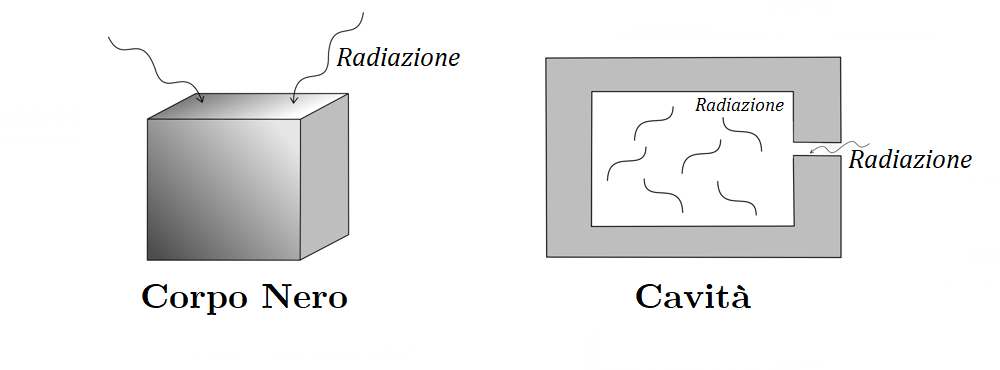
\includegraphics[width=\textwidth]{immagini/cap_1/fig_1_1.png}
\end{figure}\\
Il problema nello studio del potere emissivo del corpo nero era rappresentato dalla \textbf{discrepanza tra le osservazioni sperimentali e la descrizione teorica}.\\
\begin{figure}[!htbp]
\begin{center}
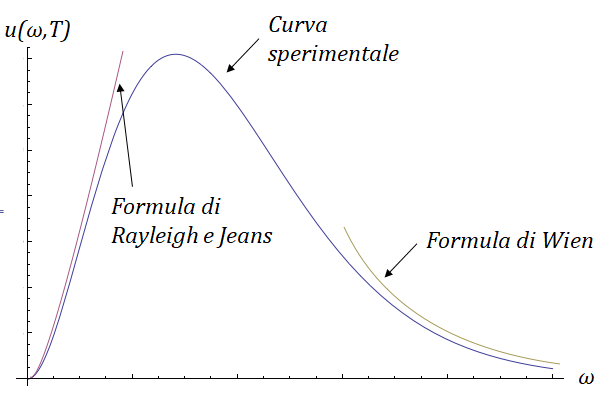
\includegraphics[width=.7\textwidth]{immagini/cap_1/fig_1_2.png}
\end{center}
\end{figure}
La descrizione teorica dello spettro di energia del corpo nero riguardava due regioni: \textbf{a basse frequenze} risultava valida la previsione della fisica classica, espressa dalla cosiddetta \textbf{formula di Rayleigh-Jeans}:
\begin{equation}
u(\omega , T)= \frac{\omega ^2}{\pi ^2 c^3}KT \qquad \textrm{ \footnotesize{(piccoli $\omega$)} }
\end{equation}
dove $K$ è la costante di Boltzmann e c la velocità della luce.\\
Ad alte frequenze risultava invece valida una formula empirica, senza alcuna interpretazione teorica, detta \textbf{formula di Wien}:
\begin{equation}
u(\omega ,T)= C \omega ^3 e^{-\lambda \omega /T} \qquad \textrm{\footnotesize{(grandi $\omega$)}}
\end{equation}
con $C$ e $\lambda$ costanti. Come è mostrato in figura, né la formula classica, né  la formula empirica di Wien descrivevano la distribuzione spettrale nella regione di frequenze intermedie.
Nel \textbf{1900, Max Planck} derivò la sua famosa formula per lo spettro di corpo nero mediante un'ingegnosa interpolazione tra la formula di Rayleigh-Jeans e la formula di Wien. La \textbf{formula}, suggerita da\textbf{Planck},
\begin{equation}
u(\omega, T) = \frac{\hbar}{\pi ^2 c^3}\frac{\omega ^3}{e^{\hbar \omega / KT}-1},
\end{equation}
risultava in perfetto accordo con le misure sperimentali. Il valore ottenuto per la \textbf{\textit{costante di Planck}} è
\[ \hbar = 1.054 \cdot 10^{-27} \ erg\cdot s.\]
Questa costante giocherà un ruolo fondamentale nella meccanica quantistica.
È immediato verificare come nei limiti di basse ed alte frequenze la formula di Planck riproduce correttamente gli andamenti già noti:\\
\begin{equation}
u(\omega , T) =\frac{\hbar}{\pi ^2 c^2} \frac{\omega ^3}{e^{\frac{\hbar \omega}{KT}} -1} 
\begin{array}{clcc}
 & \displaystyle{\frac{\omega ^2}{\pi ^2 c^3} } & \textrm{per } \hbar \omega \ll KT, & \textrm{[Rayleigh-Jeans]}\\
\nearrow \\
\searrow \\
 & \displaystyle{\frac{h}{\pi ^2 c^3}\omega ^3 e^{\frac{-\hbar \omega}{KT}}} & \textrm{per }  \hbar \omega \gg KT .& \textrm{[Wien]}
\end{array}
\end{equation}
Il perfetto accordo della sua formula indusse Planck a cercare una \textbf{spiegazione teorica}. Per comprendere la spiegazione trovata da Planck è utile discutere prima la derivazione della formula di Rayleigh-Jeans ottenuta utilizzando le leggi della fisica classica. Osserviamo anche che la formula di  Rayleigh-Jeans non poteva comunque, in generale, essere corretta perché conduce ad una densità di energia totale (integrata su tutte le frequenze) infinita (\textit{catastrofe ultravioletta})
\begin{equation}
E(T) = \int _0 ^\infty d\omega\ u(\omega , T) \overset{R.J.}{=} \frac{KT}{\pi ^2 c ^3}\int _0 ^\infty d\omega \ \omega ^2 = \infty \textrm{(!)}
\end{equation}
La formula classica di Rayleigh-Jeans era derivata calcolando il numero di modi normali di oscillazione della radiazione elettromagnetica con frequenza compresa tra $\omega$ ed $\omega + d\omega$ ed associando a ciascun modo un'energia media $KT$ (in accordo con la legge classica di equipartizione dell'energia). Discutiamo la derivazione di entrambi questi risultati.\\
Calcoliamo il numero di modi normali di oscillazione della radiazione elettromagnetica con frequenza compresa tra $\omega$ ed $\omega + d\omega$. \\
Un'onda che si propaga nella direzione $x$ con vettore d'onda $k_x$, è descritta dalla funzione $e^{ik_x x}$. Se consideriamo per il campo e.m. nella cavità con volume finito condizioni al bordo periodiche, allora il vettore d'onda $k_x$ è soggetto alla condizione:
\begin{eqnarray}
e^{ik_x x}= e^{ik_x (x+L)} \Rightarrow e^{ik_x L}=1  \nonumber\\ \Rightarrow k_x=\frac{2\pi}{L}n, \qquad n= 0, \pm 1, \pm 2,...
\end{eqnarray}
dove $L$ è la lunghezza del volume nella direzione $x$. Il numero $dn_x$ di modi normali di oscillazione con vettore d'onda $k_x$ compreso tra $k_x$ e $k_x+dk_x$ è allora:
\begin{equation}
dn_x =\frac{L}{2\pi}dk_x.
\end{equation}
Considerando le 3 direzioni spaziali del vettore d'onda ed i fatto che per ciascun' onda di vettore $\vec{k}$ esistono 2 gradi di polarizzazione indipendenti otteniamo per il numero totale di oscillazioni con frequenza compresa tra $\omega$ e $\omega + d\omega$ il valore
\begin{equation}
dn =2\frac{V}{(2\pi)^3}d^3k= V \frac{2\cdot 4\pi}{8\pi ^3} k^2 dk \overset{\omega =ck}{=} V \left( \frac{\omega ^2}{\pi ^2 c^3}\right) d\omega
\end{equation}
il primo fattore che entra nella formula di Rayleigh-Jeans,
\begin{equation}
\left( \frac{\omega ^2}{\pi ^2 c^3} \right)
\label{eq:cap1_1}
\end{equation}
rappresenta dunque il \textbf{numero di modi normali di oscillazione della radiazione, per unità di volume, con frequenza compresa tra $\omega$ e $\omega + d\omega$}.\\
Dimostriamo ora come il secondo fattore, $KT$, rappresenti secondo la fisica classica l'energia media di ciascun oscillatore armonico. A tale scopo è necessario introdurre alcuni concetti di \textbf{meccanica statistica}.\\
Secondo la meccanica statistica, la probabilità che un sistema mantenuto in equilibrio in equilibrio termico alla temperatura $T$ si trovi in uno stato $s$ corrispondente ad un'energia $E_s$ è data da:
\begin{equation}
p(E_s) =\frac{1}{z}e^{\frac{-E_s}{KT}}
\end{equation}
dove $Z$, detta funzione di partizione, è l'opportuna costante di normalizzazione della probabilità:
\begin{equation}
Z= \sum _s e^{-E_s / KT}
\end{equation} 
la sommatoria su $s$ è estesa qui a tutti i possibili stati microscopici del sistema.
Da quanto detto segue anche che l'energia media del sistema, mantenuto in equilibrio alla temperatura $T$, è data da:
\begin{equation}
\langle E \rangle = \sum _s p(E_s)\cdot E_s = \frac{1}{Z}\sum _s E_s e^{-\frac{E_s}{KT}}
\end{equation}
Applichiamo questi ora questi concetti per calcolare l'energia media di un oscillatore armonico unidimensionale in equilibrio alla temperatura $T$. L'Hamiltioniano dell'oscillatore è:
\begin{equation}
H= \frac{p^2}{2m}+\frac{1}{2}m \omega ^2 x^2
\end{equation}
e la \textit{somma sugli stati} dell'oscillatore è un integrale su tutti i possibili valori di impulso e posizione:
\begin{equation}
\sum _s = \iint dp dx
\end{equation}
L'energia media dell'oscillatore è allora: ($\beta = 1/KT$)
\begin{eqnarray}
\langle E \rangle &=& \frac{\int _{-\infty} ^{+\infty} dp dx \quad e^{-\beta \left( \frac{p^2}{2m}+\frac{1}{2}m \omega ^2x^2\right)}\left( \frac{p^2}{2m}+\frac{1}{2}m \omega ^2x^2\right)}{\int _{-\infty} ^{+\infty} dp dx e^{-\beta \left( \frac{p^2}{2m}+\frac{1}{2}m \omega ^2x^2\right)}}= \nonumber \\
&=&\frac{\int _{-\infty} ^{+\infty} dp \quad e^{-\beta \left( \frac{p^2}{2m}\right)}\left( \frac{p^2}{2m}\right)}{\int _{-\infty} ^{+\infty} dp \quad e^{-\beta \left( \frac{p^2}{2m}\right)}} + \frac{\int _{-\infty} ^{+\infty}  dx \quad e^{-\beta \left(\frac{1}{2}m \omega ^2x^2\right)}\left(\frac{1}{2}m \omega ^2x^2\right)}{\int _{-\infty} ^{+\infty} dx e^{-\beta \left( \frac{1}{2}m \omega ^2x^2\right)}}= \nonumber \\
&=& \left[ s=\frac{p}{\sqrt{2m}}; s= \sqrt{\frac{m \omega ^2}{2}x} \right]= 2\cdot \frac{\int _{-\infty} ^{+\infty}ds \quad e^{-\beta s^2}s^2}{\int _{-\infty} ^{+\infty}ds \quad e^{-\beta s^2}}= \nonumber \\
&=&-2 \frac{\partial}{\partial \beta} \ln \left(\int _{-\infty} ^{+\infty}ds \quad e^{-\beta s^2} \right) = -2\frac{\partial}{\partial \beta} \ln \sqrt{\frac{\pi}{\beta}}= \nonumber \\
&=& \frac{\partial}{\partial \beta} \ln \beta = \frac{1}{\beta}= KT. 
\end{eqnarray}
Troviamo dunque il risultato cercato:
\begin{equation}
\langle E \rangle = KT.
\label{eq:cap1_2}
\end{equation}
moltiplicando questa energia media di ciascun oscillatore per il numero di oscillatori (eq. (\ref{eq:cap1_1})) si ottiene la formula di Rayleigh-Jeans.\\
Planck trovò che la sua formula  per lo spettro di corpo nero poteva essere derivata assumendo che l'energia associata con ciascun modo del campo elettromagnetico non può variare con continuità, come predetto dalla fisica classica, ($E= p^2/2m +1/2 \ m \omega ^2 x^2$), ma deve essere un multiplo intero di un \textbf{\textit{quanto}} minimo di energia $\varepsilon$, legato alla frequenza $\omega$ del modo normale da:
\begin{equation}
\varepsilon = \hbar \omega .
\end{equation}
L'energia ha dunque forma:
\begin{equation}
E_n = n\varepsilon = n \hbar \omega \quad n= 0,1,2...
\end{equation}
In questo caso infatti, l'energia media associata a ciascun modo normale a temperatura $T$ è data da:
\begin{eqnarray}
\langle E \rangle &=&\sum _n p(E_n) E_n =\frac{1}{Z}\sum _n ^{\infty} e^{-\beta n \hbar \omega} \cdot n\hbar \omega = \nonumber \\
&=&\frac{\sum _n ^{\infty} e^{-\beta n \hbar \omega} \cdot n\hbar \omega}{\sum _n ^{\infty} e^{-\beta n \hbar \omega}}= - \frac{\partial}{\partial \beta} \ln \left( \sum _n ^{\infty} e^{-\beta n \hbar \omega}\right)= \nonumber \\
&=&- \frac{\partial}{\partial \beta} \ln \left( \frac{1}{1- e^{-\beta \hbar \omega}}\right)=  \frac{e^{-\beta \hbar \omega}\ \hbar \omega}{1-e^{-\beta \hbar \omega}}= \frac{ \hbar \omega}{e^{\beta \hbar \omega}-1}\nonumber \\
&\textrm{ossia}& \quad \langle E \rangle = \frac{ \hbar \omega}{e^{\beta \hbar \omega}-1}.
\end{eqnarray}
Questa energia, moltiplicata per il numero di modi normali per unità di volume con frequenza compresa tra $\omega$ ed $\omega + d\omega$, fornito dalla formula (\ref{eq:cap1_1}), conduce alla formula di Planck.\\
Lo spettro di corpo nero sembrava dunque indicare che la \textbf{la radiazione elettromagnetica si comporta come se fosse costituita da un insieme di quanti di energia con energia pari ad $\hbar \omega $.}
L'origine di questo comportamento risultava però ancora oscuro. Il passo successivo, che contribuì a chiarire la conclusione di Planck, si ebbe cinque anni dopo, con l'interpretazione fornita da Einstein dell'effetto fotoelettrico.
\section{L'effetto fotoelettrico}
L'effetto fotoelettrico, scoperto nel 1887 da Hertz, venne spiegato da \textbf{Einstein} nel \textbf{1905} utilizzando il concetto di natura quantistica (corpuscolare) della luce.\\
L'\textbf{effetto fotoelettrico} può essere riassunto nel modo seguente:
\begin{enumerate}
\item Quando una superficie metallica viene investita da un'onda luminosa può emettere elettroni;
\item  l'emissione o meno di elettroni dipende dalla frequenza della luce incidente. In generale esiste una \textbf{soglia} (che varia da metallo a metallo) per cui solo frequenze maggiori della soglia producono la corrente fotoelettrica;
\item l' \textbf{intensità della corrente}, quando esiste, è proporzionale all'intensità della radiazione luminosa;
\item l'\textbf{energia dei fotoelettroni} è indipendente dall'intensità della luce ma varia linearmente con la frequenza della luce incidente.
\end{enumerate} 
\textbf{Classicamente, l'effetto fotoelettrico risulta inspiegabile}. Secondo l'elettrodinamica classica, infatti, l'energia trasportata da un'onda elettromagnetica è proporzionale all'intensità dell'onda, ed indipendente dalla frequenza. Non è possibile pertanto spiegare perché l'effetto abbia una soglia dipendente dalla frequenza e perché l'energia dei fotoelettroni dipenda dalla frequenza.\\
Per spiegare l'effetto fotoelettrico \textbf{Einstein partì dall'ipotesi che la radiazione luminosa è costituita da quanti di energia $\hbar \omega$}, dove $\omega$ è la frequenza della luce.\\
\textbf{L'assorbimento da parte di un elettrone del metallo si un singolo quanto di luce}, o fotone, come venne in seguito chiamato, accresce l'energia dell'elettrone di una quantità $\hbar \omega$.\\
una parte di questa energia, $W$, detta \textbf{funzione lavoro}, deve essere spesa per separare l'elettrone dal metallo. Questa energia varia da metallo a metallo. L'energia restante è disponibile come energia cinetica dell'elettrone fotoemesso. La \textbf{conservazione dell'energia} nel processo implica pertanto la seguente relazione tra la velocità dell'elettrone $v$ e la frequenza $\omega$ della luce:
\begin{equation}
\frac{1}{2}m v^2= \hbar - W.
\end{equation}
La presenza di una soglia e la relazione lineare tra energia dell'elettrone e frequenza sono contenute in questa formula.\\ La proporzionalità tra la corrente fotoelettrica ed intensità della sorgente luminosa può pure essere spiegata in termini di quanti di luce: una sorgente di luce più intensa emette più fotoni e questi, a loro volta, liberano più elettroni.\\ La correttezza della formula di Einstein venne verificata in una serie di esperimenti, in particolare da \textbf{Millikan}. L'effetto fotoelettrico venne così a costituire una delle forti evidenze sperimentali a favore della natura corpuscolare della luce.
\section{L'effetto Compton}
L'\textbf{effetto Compton} (1922) è forse il fenomeno fisico che, più di ogni altro, ha fornito un'evidenza diretta della natura corpuscolare della luce.\\ \textbf{Compton scoprì che la radiazione di una certa lunghezza d'onda} (nella regione dei raggi x) \textbf{fatta incidere su di un foglio metallico, veniva diffusa con lunghezza d'onda differente dalla lunghezza d'onda della luce incidente, e la differenza delle lunghezze d'onda dipendeva dall'angolo di diffusione}.\\
Secondo \textbf{l'elettrodinamica classica}, la diffusione della luce è dovuta all'irraggiamento da parte degli elettroni atomici, che vengono posti in oscillazioni forzate dalla luce incidente. In questo caso la lunghezza d'onda diffusa è prevista essere uguale alla lunghezza d'onda della luce incidente e l'intensità ha una dipendenza dall'angolo $\theta$ di diffusione dato da $(1+cos^2 \theta)$ (\textbf{scattering Thomson}).\\
Lo spostamento osservato nella lunghezza d'onda della luce diffusa viene spiegato da Compton considerando la radiazione incidente come fascio di fotoni di energia $\hbar \omega$. \textbf{I singoli fotoni vengono diffusi elasticamente dai singoli elettroni:}\\
\begin{figure}[!htbp]
\begin{center}
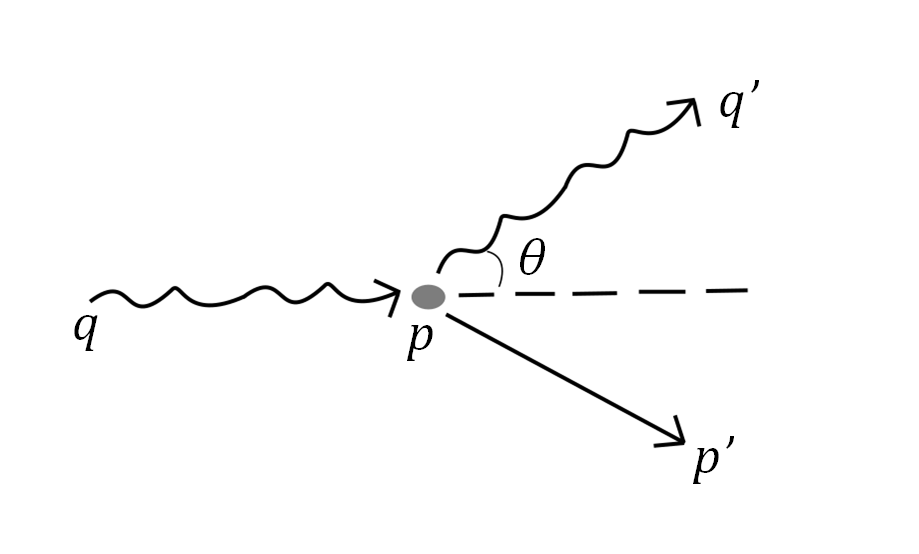
\includegraphics[width=.6\textwidth]{immagini/cap_1/fig_1_3.png}
\end{center}
\end{figure}\\
Un fotone di frequenza $\omega$ e vettore d'onda $\vec{k}$ ha energia $E = \hbar \omega$ ed impulso $\vec{q}= \hbar \vec{k}$. La relazione relativistica $E=cq$, valida per particelle di massa nulla, implica $\omega = c|\vec{k}|$. I 4-vettori energia.impulso per il fattore incidente ed il fotone diffuso hanno dunque la forma:
\begin{equation}
q=\left(\frac{\bar \omega}{c}; \hbar \vec{k} \right)\qquad q' = \left(\frac{\bar \omega'}{c}; \hbar \vec{k'} \right),
\end{equation}
e si ha:
\begin{equation}
q^2 = q'^2=0.
\end{equation}
Poiché l'elettrone si trova inizialmente in quiete il suo 4-vettore energia-impulso è dato da:
\begin{equation}
p=\left(mc, \vec{0} \right)\qquad p^2 =m^2 c^2.
\end{equation}
La legge di \textbf{conservazione del 4-impulso} nel processo si scrive:
\begin{equation}
p+q=p'+q',
\end{equation}
da cui:
\begin{eqnarray}
p'^2 &=& m^2 c^ = \left( p +q -q'\right)^2= p^2 + q^2 +q'^2+ 2pq - 2pq' -2 qq'= \nonumber \\
&=& m^2c^2 + 2m\hbar \omega - 2m \hbar \omega ' - 2 \frac{\hbar \ \omega \omega '}{c^2}+2 \hbar \ k k'  \cos \theta ,
\end{eqnarray}
ossia:
\begin{equation}
\omega - \omega ' =\frac{\hbar}{m c^2} \omega \omega ' \left( 1-\cos \theta \right).
\label{eq:cap1_3}
\end{equation}
\begin{center}
\fbox{\begin{minipage}{.9\textwidth}
\textbf{Cinematica effetto Compton}: calcolo non esplicitamente relativistico\\
\begin{center}
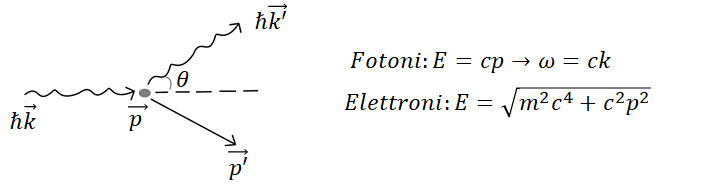
\includegraphics[width=\textwidth]{immagini/cap_1/fig_1_4.png}
\end{center}
\begin{equation}
\left\{
\begin{aligned}
&\hbar \omega +m c^2 = \hbar \omega ' +\sqrt{m^2 c^4 + c^2 p'^2}\quad \textrm{Cons. dell'energia (1)}\\
& \hbar \vec{k} = \hbar \vec{k'} + \vec{p'}\qquad \qquad \qquad \qquad \quad \textrm{Cons. dell'impulso (2)}
\end{aligned}
\right.
\end{equation}
\begin{eqnarray}
c^2 p'^2 &\overset{\textrm{(2)}}{=}& c^2\hbar^2 \left( \vec{k}- \vec{k'} \right) ^2 = \hbar ^2 c^2 \left(k^2+k'^2-2kk' \cos \theta \right) \nonumber \\
&=& \hbar ^2 \left(\omega ^2 + \omega ^2 - 2 \omega \omega ' \cos \theta  \right)\overset{\textrm{(1)}}{=} \nonumber \\
&=& \left( \hbar \omega - \hbar \omega ' + m c^2 \right) ^2 - m^2 c^4= \nonumber \\
&=& {\hbar}^2 \left({\omega}^2 + {\omega '} ^2 - 2 \omega \omega ' \right) + 2 mc^2 \hbar ( \omega - \omega ' ) \Rightarrow \nonumber \\
&\Rightarrow & \omega - \omega' =\frac{\hbar}{m c^2} \omega \omega ' \left( 1- \cos \theta \right).
\end{eqnarray}
\end{minipage}}
\end{center}

Esprimiamo questo risultato in termini delle lunghezze d'onda dei fotoni incidente e diffuso. Queste sono legate alle frequenze dalla relazione:
\begin{equation}
\omega = c k =\frac{2 \pi c}{\lambda} \Rightarrow \lambda =\frac{2 \pi c}{\omega},
\end{equation}
moltiplicando entrambi i membri dell'equazione (\ref{eq:cap1_3}) per $2 \pi c / \omega \omega '$ si ottiene:
\begin{equation}
\lambda - \lambda ' =\frac{h}{mc}\left( 1-\cos \theta \right),
\end{equation}
che esprime lo spostamento della lunghezza d'onda del fotone diffuso, $\lambda ' $, in termini della lunghezza d'onda del fotone incidente $\lambda$. Questa previsione risultò in perfetto accordo con i dati sperimentali.
La quantità $\hbar/ mc$, che ha dimensioni di una lunghezza, è detta \textbf{lunghezza d'onda Compton dell'elettrone} e vale:
\[
\frac{\hbar}{mc}= 2\pi \frac{e^2}{mc^2}\frac{\hbar c}{e^2}= \frac{2\pi r_0}{\alpha}= 2.4 \cdot 10^{-10} \ cm,
\]
\[(r_0 = e^2/mc = 2.82 \cdot 10^{-13} cm = \textrm{raggio classico dell'elettrone}\]
\[\alpha = e^2/\hbar c = 1/137 = \textrm{costante di struttura fine}).\]
L'interpretazione dell'effetto Compton fornì l' \textbf{evidenza definitiva del comportamento corpuscolare della luce}. Poiché la radiazione elettromagnetica presenta anche proprietà ondulatorie, e dà luogo a fenomeni di interferenza e diffrazione, questi risultati dovevano portare ad un radicale cambiamento delle leggi classiche.
\section{Diffrazione degli elettroni}
\textbf{Nel 1923 De Broglie avanzò l'ipotesi che la natura duale onda-particella della radiazione avesse la sua controparte in una natura duale onda-particella della materia}.\\
Per un fotone la relazione tra impulso e lunghezza d'onda è data da:
\begin{equation}
p= \hbar k = \frac{2\pi \hbar}{\lambda}=\frac{h}{\lambda},
\end{equation}
De Broglie ipotizzò che la stessa relazione fosse valida per le particelle della materia. In altri termini una particella di impulso $p$ si comporta, sotto certe condizioni,come un'onda di lunghezza d'onda:
\begin{equation}
\lambda=\frac{h}{p}.
\end{equation}
Venne allora suggerito he l'ipotesi di De Broglie potesse essere verificata sperimentalmente osservando il fenomeno di \textbf{diffrazione degli elettroni}.\\
La diffrazione degli elettroni venne osservata in una serie di \textbf{esperimenti} da \textbf{Davisson e Germer}, che studiarono la \textbf{diffusione degli elettroni da una superficie di un cristallo}:
\newpage
\begin{figure}[!htbp]
\begin{center}
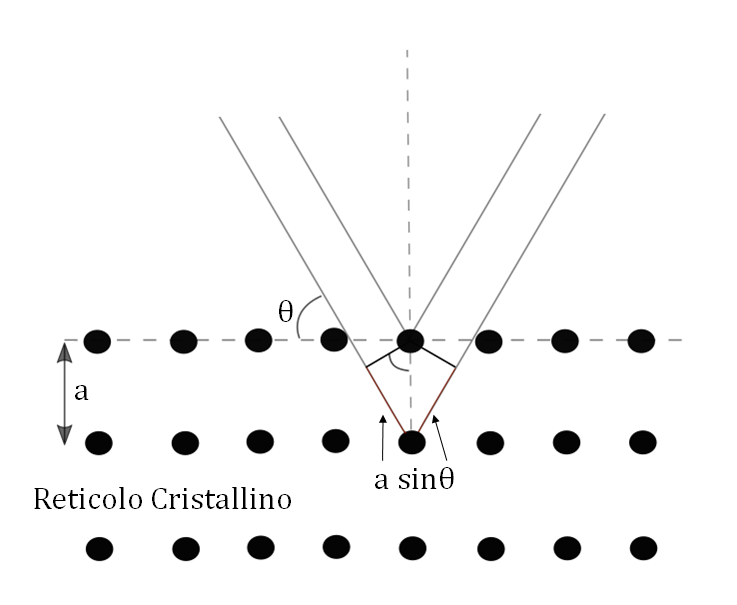
\includegraphics[width=.65\textwidth]{immagini/cap_1/fig_1_5.png}
\end{center}
\end{figure}
La differenza di fase tra due onde diffuse  da piani adiacenti del reticolo cristallino è data da:
\begin{equation}
\delta = k \Delta x = \frac{2 \pi}{\lambda} 2a \sin \theta.
\end{equation}
Si osserverà allora interferenza costruttiva quando questa differenza è pari ad un multiplo intero di $2 \pi$: $k \Delta x = 2 \pi n$, ossia:
\begin{equation}
2a \sin \theta = n\lambda.
\end{equation}
un figura di diffrazione, i cui massimi si presentano in corrispondenza degli angoli definiti dalla precedente equazione, venne effettivamente osservata negli esperimenti. la lunghezza d'onda, associata ad elettroni di impulso $p$, risultò inoltre in accordo con la formula di De Broglie. Questa osservazione rappresentò pertanto un passo fondamentale nella formulazione della \textbf{meccanica ondulatoria}.
\section{L'esperimento di Rutherford e gli spettri atomici}
Nel 1908 \textbf{Rutherford} effettuò un \textbf{esperimento per studiare la struttura atomica.} L'esperimento consisteva nel bombardare sottili fogli di metallo con particelle $\alpha$, prodotte dal decadimento radioattivo. Il risultato inatteso fu che una significativa frazione di particelle $\alpha$ veniva deviata a grandi angoli di diffusione.\\
Il risultato dell'esperimento di Rutherford era inconsistente con le aspettative basate sul \textbf{modello di Thomson} dell'atomo. In questo modello si ipotizzavano gli elettroni immersi in una distribuzione di carica positiva, la cui estensione determina le dimensioni dell'atomo. Tuttavia gli elettroni non deviano le particelle $\alpha$, avendo una massa circa $10^4$ volte più piccola. Pertanto la sorgente che diffonde le particelle $\alpha$ deve essere la carica positiva, e grandi angoli di diffusione implicano che il potenziale sulla superficie della distribuzione di carica è grande. Questo a sua volta implica che la carica positiva è confinata in una regione di spazio molto più piccola dell'atomo.\\
\textbf{Rutherford} propose un \textbf{nuovo modello} in grado di spiegare i dati. In questo modello tutta la carica positiva (e quasi tua la massa) è concentrata in una piccola regione al centro dell'atomo. Questo nucleo d carica positiva attrae gli elettroni, carichi negativamente e, poiché la legge di forza ha un andamento $1/r^2$, \textbf{gli elettroni si muovono in orbite circolari od ellittiche attorno a nucleo.}\\
sebbene in grado di spiegare i dati sperimentali relativi alla diffusione delle particelle $\alpha$, il modello di Rutherford presentava \textbf{due insuperabili difficoltà:}
\begin{itemize}
\item \textbf{Manca un meccanismo per stabilizzare gli atomi}: gli elettroni in orbite circolari od ellittiche sono costantemente accelerati e, secondo la teoria elettrodinamica classica, dovrebbero irradiare. La continua perdita di energia condurrebbe, in un tempo molto breve (dell'ordine di $10^{-10}$ s) al collasso dell'atomo con gli elettroni che cadono sopra il nucleo;
\item Il modello non è in grado di spiegare gli \textbf{spettri atomici}, che si osservavano avere la struttura
\begin{equation}
\frac{1}{\lambda} = cost. \left( \frac{1}{n_1 ^2}-\frac{1}{n_2 ^2} \right),
\end{equation}
dove $n_1$ ed $n_2$ sono numeri interi.
\end{itemize}
Queste evidenti difficoltà tecniche nell'interpretazione dei risultati sperimentali relativi alla struttura atomica giocarono un ruolo fondamentale nello sviluppo della teoria quantistica.%DEFINITIVO
\chapter[Principi fondamentali della M.Q.]{Principi fondamentali\\ della Meccanica \\ Quantistica. Dualismo\\ onda-particella,\\ probabilità ed ampiezze\\ di probabilità, onde ed\\ elettroni\footnote{F1.1-1.8; LL1}}
La \textbf{meccanica quantistica} è la descrizione del comportamento della materia e della luce in tutti i suoi dettagli ed in particolare di ciò che avviene su scala atomica.\\
\textbf{Gli oggetti su scala molto piccola non i comportano come nessuna cosa di cui si possa avere diretta esperienza.} Sotto alcuni aspetti si comportano come onde, sotto altri come particelle, ma in effetti non si comportano come né l'una né l'altra cosa.\\
D'altra parte il \textbf{comportamento quantistico degli oggetti atomici} (elettroni, protoni, neutroni, fotoni e così via) \textbf{è lo stesso per tutti}: sono tutti \textit{onde-particelle}, o qualunque altro nome gli si voglia dare. onde-particelle. \textbf{Una descrizione coerente del comportamento della materia su scala microscopica venne dato, negli anni 1926-1927, principalmente da Schr\"{o}dinger, Heisenberg e Born.}\\
Consideriamo qui le principali caratteristiche di tale descrizione, descrivendo un \textbf{esperimento ideale}, che mette a confronto una particolare situazione sperimentale, il comportamento quantistico degli elettroni con il comportamento d particelle classiche, quali pallottole, ed onde classiche, del tipo di quelle che si formano nell'acqua.
\newpage
\section*{Un esperimento con pallottole}
\begin{figure}[!htbp]
\begin{center}
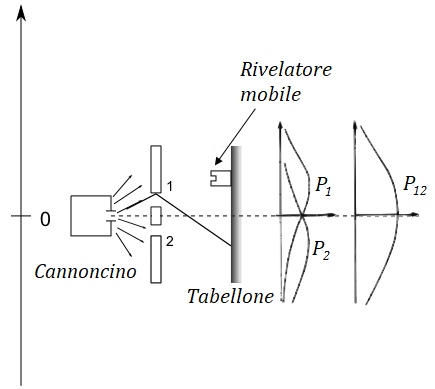
\includegraphics[width=.6\textwidth]{immagini/cap_2/fig_2_1.png}
\end{center}
\end{figure}
\begin{itemize}
\item[\textbf{P$_1=$} ]probabilità che il proiettile giunga in $x$ passando per il foro 1;
\item[\textbf{P$_2=$} ]probabilità che il proiettile giunga in $x$ passando per il foro 2;
\item[\textbf{P$_{12}=$} ]probabilità che il proiettile giunga in $x$ passando per il foro 1 o per il foro 2.
\end{itemize}
\textbf{Risultato dell'esperimento:} I proiettili arrivano sempre a blocchi identici e distinti. L'effetto con entrambi i fori aperti è la somma degli effetti che si hanno quando è aperto ciascuno dei sue fori da solo. Le probabilità vanno sommate:
\begin{equation}
P_{12}=P_1+P_2.
\end{equation}
\textbf{Non si osserva interferenza.}
\newpage
\section*{Un esperimento con onde (prodotte in acqua)}
\begin{figure}[!htbp]
\begin{center}
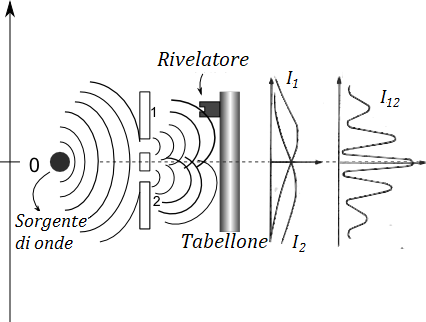
\includegraphics[width=.6\textwidth]{immagini/cap_2/fig_2_2.png}
\end{center}
\end{figure}
\begin{itemize}
\item[\textbf{I$_1=$} ]intensità misurata lasciando aperto solo il foro 1;
\item[\textbf{I$_2=$} ]intensità misurata lasciando aperto solo il foro 2;
\item[\textbf{I$_{12}=$} ]intensità misurata lasciando aperti entrambi i fori.
\end{itemize}
\textbf{Risultato dell'esperimento:} l'intensità  può assumere qualsiasi valore; non possiede una struttura \textit{a blocchi}. \textbf{L'intensità} misurata quando entrambi i fori sono aperti \textbf{non è la somma} di I$_1$ e I$_2$: \textbf{si ha interferenza tra le due onde.}
\subsection*{Matematica dell'interferenza (formalismo complesso)}
\begin{itemize}
\item $\Re{\left(h_1 e^{i\omega t} \right)}=$ altezza istantanea al rivelatore dell'onda proveniente dal foro 1;
\item $\Re{\left(h_2 e^{i\omega t} \right)}=$ altezza istantanea al rivelatore dell'onda proveniente dal foro 2;
\item $\Re{\left( \left(h_1 +h_2 \right) e^{i\omega t} \right)}=$ altezza istantanea al rivelatore dell'onda che arriva quando entrambi i fori sono aperti.
\end{itemize}
L'intensità è proporzionale all'ampiezza quadratica media, cioè, con il famoso formalismo complesso, al modulo quadro dell'ampiezza. Tralasciando la costante di proporzionalità:
\begin{eqnarray}
& &I_1= \lvert {h_1} \rvert ^2, \nonumber \\
& &I_2 \lvert {h_1} \rvert ^2, \\
& &I_{12}= \lvert {h_1+h_2} \rvert ^2= \lvert {h_1} \rvert ^2+ \lvert {h_2} \rvert ^2 + 2 \lvert {h_1} \rvert \lvert {h_2} \rvert \cos \delta ,\nonumber  \\ 
& &\left( \delta = \textrm{ differenza di fase tra } h_1 \textrm{ e } h_2 \textrm{, funzione di }x \right)\nonumber 
\end{eqnarray}
allora, in termini di intensità:
\begin{equation}
I_{12}= I_1 + i_2 + 2 \sqrt{I_1 I_2}\cos \delta.
\end{equation}
L'ultimo termine in questa espressione è il \textbf{termine di interferenza.}
\section*{Un esperimento con elettroni}
\begin{figure}[!htbp]
\begin{center}
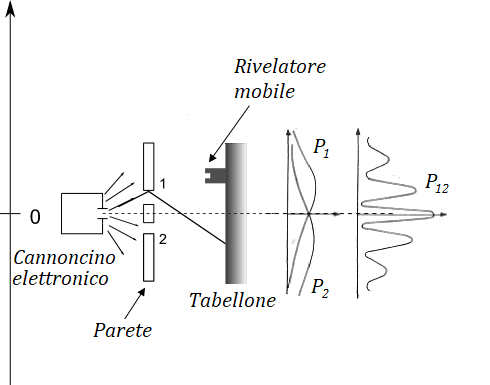
\includegraphics[width=.6\textwidth]{immagini/cap_2/fig_2_3.png}
\end{center}
\end{figure}
\begin{itemize}
\item[\textbf{P$_1=$} ]probabilità che l'elettrone giunga in $x$ passando per il foro 1 (con il foro 2 chiuso);
\item[\textbf{P$_2=$} ]probabilità che l'elettrone giunga in $x$ passando per il foro 2 (con il foro 1 chiuso);
\item[\textbf{P$_{12}=$} ]probabilità che il proiettile giunga in $x$ con entrambi i fori aperti.
\end{itemize}
\textbf{Risultato dell'esperimento:} I proiettili arrivano sempre in granuli, tutti identici tra loro (come i proiettili). La \textbf{probabilità} $P_{12}$ ottenuta con entrambi i fori aperti non è la somma di $P_1$ e $P_2$:
\begin{equation}
P_{12}\neq P_1+P_2.
\end{equation}
Se fosse vero che ciascun elettrone o attraversa il foro 1 oppure attraversa il foro  allora la probabilità $P_{12}$ dovrebbe essere la somma di $P_1$ e $P_2$. Si potrebbe pensare che gli elettroni seguano percorsi complicati, passando magari più volte per ciascun foro. Ma nemmeno questo è possibile:
\begin{itemize}
\item \textbf{vi sono punti n cui} arrivano meno elettroni quando sono aperti entrambi i fori, ossia \textbf{la chiusura di un foro aumenta il numero di elettroni provenienti dall'altro;}
\item \textbf{al centro della curva}, $P_{12}$ è maggiore della somma $P_1 + P_2$,  \textbf{è come se la chiusura di un foro diminuisce il numero di elettroni che escono dall'altro}.
\end{itemize}
Sebbene questi risultati siano incomprensibili, la loro descrizione matematica è estremamente semplice: \textbf{la curva $P_{12}$ è proprio una curva di interferenza come $I_{12}$ e la matematica è dunque quella dell'interferenza.}\\
I risultati dell'esperimento possono essere descritti introducendo due numei complessi, funzione di $\chi$: $\phi _1$ e $\phi _2$. Si ha poi:
\begin{eqnarray}
& P_1= \lvert \phi _1 \rvert ^2, & \\
& P_2= \lvert \phi _2 \rvert ^2, &\\
& P_{12}= \lvert \phi _1 + \phi _2 \rvert ^2. 
\end{eqnarray}
\section*{Osservazione di elettroni}
Poiché il numero di elettroni che arriva in un particolare punto \textbf{non} è uguale al numero di elettroni che arrivano passando dal foro 1 più quelli che passano dal foro 2 ci porta a concludere che \textbf{non è vero che gli elettroni passano attraverso l'uno o l'altro dei fori 1 e 2}. Verifichiamo questa conclusione con un esperimento.\\
Aggiungiamo nell'apparato sperimentale una sorgente di luce, posa dietro allo schermo, a metà tra i due fori. Poiché le cariche elettriche diffondono la luce, quando un elettrone riesce ad attraversare lo schermo devierà verso il nostro occhio della luce e potremo \textit{vedere} il cammino dell'elettrone stesso.
\newpage
\begin{figure}[!htbp]
\begin{center}
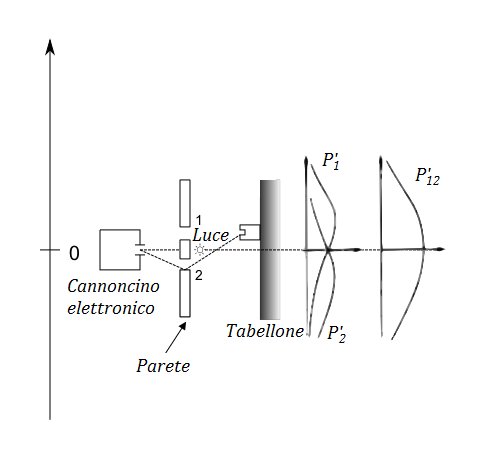
\includegraphics[width=.6\textwidth]{immagini/cap_2/fig_2_4.png}
\end{center}
\end{figure}
\textbf{Risultato dell'esperimento:} Gli elettroni che vengono osservati risultano essere passati o dal foro 1 o dal foro 2 ma non da tutti e due insieme. L'andamento di $P'_1$ e $P'_2$, costruiti lasciando entrambi i fori aperti ma osservando da quale foro sia passato l'elettrone è uguale all'andamento di $P_1$ e $P_2$ osservato nel precedente esperimento chiudendo uno dei due fori. Quindi \textbf{gli elettroni che vediamo arrivare attraverso il foro 1 sono distribuiti nello stesso modo, indipendentemente dalla situazione del foro 2.}\\
La probabilità totale risulta dunque essere la somma delle probabilità
\begin{equation}
P'_{12}= P'_1 + P'_2.
\end{equation}
\textbf{La distribuzione degli elettroni sullo schermo quando li osserviamo è differente da quella quando non li osserviamo}.\\
Evidentemente la luce, nell'essere diffusa dagli elettroni, dà loro un colpo che ne fa mutare il movimento. Si può tentare allora di modificare l'esperimento in modo da osservare gli elettroni senza disturbarli troppo. Ma questo non risulta essere possibile. \textbf{È impossibile costruire un apparecchio per determinare da quale foro è passato l'elettrone che allo stesso tempo non perturbi l'elettrone sufficientemente da distruggere l'interferenza. se un apparecchio è capace di determinare da quale foro è passato l'elettrone  non può essere così delicato da non alterarne in modo essenziale la distribuzione.} Questo risultato è una conseguenza particolare del \textbf{principio di indeterminazione.}
\section[Probabilità e ampiezza di probabilità]{Principi base della Meccanica quantistica: probabilità e ampiezza di probabilità}
Riassumiamo ora, in forma generale le principali conclusioni dell'esperimento sopra descritto:
\begin{enumerate}
\item La probabilità di un evento in un esperimento ideale è data dal quadrato del modulo d un numero complesso $\phi$ che viene detto \textbf{ampiezza di probabilità:}
\begin{eqnarray}
& & P = \textrm{ probabilità}, \nonumber \\
& & \phi = \textrm{ ampiezza di probabilità}, \nonumber \\
& & P = \lvert \phi \rvert ^2 .
\end{eqnarray}
\item Quando un evento può avvenire secondo varie alternative, l'ampiezza di probabilità per l'evento è la somma delle ampiezze di probabilità per le varie alternative considerate separatamente. Si ha perciò interferenza:
\begin{eqnarray}
&\phi = \phi_1 + \phi _2,&  \\
&P = \lvert \phi_1 + \phi _2 \rvert ^2;&
\end{eqnarray}
\item Se si effettua un'esperienza capace di determinare se una o l'altra delle possibili alternative è effettivamente realizzata, la probabilità dell'evento non è la somma delle probabilità per ciascuna delle alternative. Non si ha più interferenza:
\begin{equation}
P= P_1 + P_2.
\end{equation}
\end{enumerate}
Sottolineiamo una differenza molto importante tra la meccanica classica e quella quantistica. \textbf{Nella meccanica quantistica è impossibile prevedere esattamente ciò che accadrà in una data situazione. la sola cosa che è possibile prevedere é la probabilità di eventi differenti.}
\section{Il principio di indeterminazione}
La presenza d interferenza nell'esperimento delle due fenditure, con gli elettroni, mette in risalto come, nel caso di particelle microscopiche, il \textbf{concetto di traiettoria}, che sta a fondamento della meccanica classica, \textbf{viene a perdere di significato nella meccanica quantistica}. Tale circostanza trova la sua espressione nel cosiddetto \textbf{principio di indeterminazione}, uno dei principi basilari della meccanica quantistica, scoperto da \textbf{Heisenberg} nel \textbf{1927}.\\
Se, in seguito ad una misura, ad un elettrone vengono assegnate coordinate determinate, esso non ha, in generale, nessuna velocità determinata. Viceversa se è dotato di una velocità determinata, l'elettrone non potrà avere una posizione determinata nello spazio. Infatti \textbf{l'esistenza simultanea ad ogni istante delle coordinate e delle velocità significherebbe l'esistenza di una traiettoria determinata, che l'elettrone non ha}. Di conseguenza nella meccanica quantistica \textbf{le coordinate e le velocità dell'elettrone sono grandezze che non possono essere misurate con precisione allo stesso istante, cioè non possono avere simultaneamente valori determinati. Si può dire che le coordinate e le velocità dell'elettrone sono grandezze non esistenti simultaneamente.}\\
Una formulazione matematica del principio di indeterminazione è data dalla relazione:
\begin{equation}
\Delta p_x \Delta x \geq \frac{\hbar}{2}.
\end{equation}
\subsection{Il principio di indeterminazione e l'esperimento delle due fenditure}
Mostriamo, in un caso particolare, come il principio di indeterminazione di Heisenberg deve essere valido al fine di evitare situazioni inconsistenti.\\
Immaginiamo di modificare l'esperimento di interferenza degli elettroni sostituendo la parete fissa, con le due fenditure, con una lamina montata su due cuscinetti che si può muovere liberamente in direzione dell'asse x:
\begin{figure}[!htbp]
\begin{center}
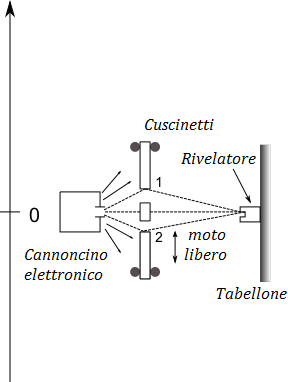
\includegraphics[width=.5\textwidth]{immagini/cap_2/fig_2_5.png}
\end{center}
\end{figure}\\
Osservando il moto della lamina possiamo provare a determinare attraverso quale foro passa un elettrone. Consideriamo infatti il caso in cui il rivelatore è posto in $x=0$. Ci aspettiamo che un elettrone che passi per il foro 1 debba essere deflesso verso il basso dalla lamina per poter arrivare al rivelatore. Poiché la componente verticale dell'impulso dell'elettrone è variata la lamina deve muoversi in direzione opposta con lo stesso impulso. La lamina riceverà quindi una spinta verso l'alto. Se invece l'elettrone passa dal foro inferiore la lamina dovrebbe subire una spinta verso il basso. È chiaro che per ogni posizione del rivelatore l'impulso ricevuto dalla lamina avrà un valore differente a seconda che l'elettrone attraversi il foro 1 o il foro 2. Quindi, \textbf{senza per nulla perturbare gli elettroni, ma solo osservando la lamina, possiamo determinare il percorso scelto dall'elettrone.\\
Tuttavia, per determinare di quanto è variato l'impulso della lamina dopo il passaggio dell'elettrone occorre conoscere l'impulso di questa prima che l'elettrone la attraversi.} Calcoliamo l'impulso che l'elettrone trasmette alla lamina attraversando un foro:\\
\begin{minipage}{.5\textwidth}
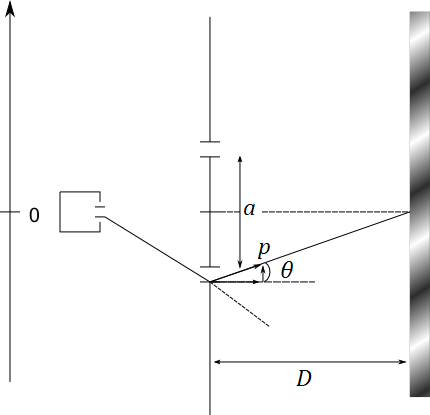
\includegraphics[width=.8\textwidth]{immagini/cap_2/fig_2_6.png}	
\end{minipage}
\hspace{.5cm}
\begin{minipage}{.4\textwidth}
\begin{equation} \tan \theta \simeq \theta \simeq \frac{a}{2D}
\end{equation}
\begin{equation} p_x = p \sin \theta = \frac{pa}{2D}
\end{equation}
\end{minipage}\\
\vspace{.5cm}
l'impulso trovato è dell'ordine di
\begin{equation}
\Delta p \simeq 2p_x = 2p \sin \theta \simeq \frac{pa}{D},
\end{equation}
e questa quantità rappresenta anche l'incertezza massima con la quale è necessario conoscere l'impulso della lacuna prima che l'elettrone l'attraversi per poter distinguere se l'elettrone è passato attraverso il foro 1 o il foro 2.\\
In base al \textbf{principio di indeterminazione}, se l'impulso è noto con una precisione maggiore di $\Delta  p$, allora \textbf{la posizione della lamina stessa non può essere conosciuta con una precisione maggiore di}:
\begin{equation}
\Delta x \simeq \frac{\hbar}{\Delta p} \simeq \frac{\hbar D}{pa}= \frac{\lambda D}{a},
\end{equation}
dove $\lambda = \hbar / p$ è la lunghezza d'onda di De Broglie associata all'elettrone che si muove con impulso $p$.\\
L'incertezza $\Delta x$ allora anche l'incertezza con cui è definita la posizione delle due fenditure, che saranno quindi in diverse posizioni per ogni elettrone che l'attraversi. Questo significa che \textbf{il centro delle frange di interferenza avrà una posizione differente per i vari elettroni.}\\
Dimostreremo ora che la lunghezza $\Delta x$, di cui oscillano lungo l'asse $x$ le frange di interferenza, è circa uguale alla distanza tra due massimi vicini. \textbf{Un tale movimento, che avviene a caso, è giusto sufficiente a distruggere le oscillazioni del grafico e quindi a far s che non si osservi più interferenza.}\\
\vspace{1cm}
\begin{minipage}{.5\textwidth}
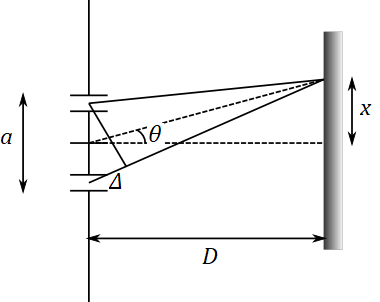
\includegraphics[width=.8\textwidth]{immagini/cap_2/fig_2_7.png}	
\end{minipage}
\begin{minipage}{.5\textwidth}
\begin{equation}
\Delta = a \sin \theta \simeq a \theta = \frac{ax}{D}
\end{equation}
\end{minipage}\\
\vspace{.5cm}
La differenza di fase tra le onde che giungono nel punto $x$ dalle due fenditure è:
\begin{equation}
\delta = k\Delta =\frac{2 \pi }{\lambda}\Delta = \frac{2 \pi a x}{D}.
\end{equation}
I massimi di interferenza si hanno quando la differenza di fase $\delta $ è pari ad un multiplo intero di $2 \pi$, ossia nei punti d coordinate
\begin{equation}
x_n =n\frac{\lambda D}{a}, \qquad n=0,\pm 1, \pm 2, \dots 
\end{equation}
Due massimi consecutivi si trovano dunque a distanza 
\begin{equation}
\Delta x = \frac{\lambda D}{a},
\end{equation}
che coincide con lo spostamento tipico del centro delle frange di interferenza per ciascun elettrone.\\
\textbf{il principio di indeterminazione garantisce quindi che l'aver osservato la fenditura attraverso la quale è passato l'elettrone porta alla scomparsa dell'interferenza.}%DEFINITIVO
\input{Capitolo_3_(Paolo)/capitolo3.tex}%DEFINITIVO
\chapter[Misure e osservabili]{Misure, osservabili e principio di indeterminazione\footnote{S1.4}}
Discutiamo qui la \textbf{teoria quantistica della misura}. In meccanica quantistica, per un sistema che si trovi in un determinato stato iniziale $\vert \varphi \rangle$, una misura di una quantità fisica non produce,in generale, sempre lo stesso risultato. Piuttosto si possono ottenere differenti risultati, ciascuno con una determinata probabilità.\\
Se indichiamo con $a_i$ i possibili risultati di una misura dell'osservabile $A$ e con $P_i$ le relative probabilità (riferite ad un sistema che si trovi nello stato $\vert \varphi \rangle$) possiamo scrivere il \textbf{valore medio} dei risultati di una misura $A$ come
\begin{equation}
\langle A \rangle = \sum _i a_i P_i.
\end{equation}
\textbf{Nella meccanica quantistica si associa ad ogni grandezza fisica $A$ un operatore lineare che la rappresenta:}

\begin{equation}
\begin{array}{c}
\textrm{Grandezza fisica}\\
A
\end{array}
\longleftrightarrow
\begin{array}{c}
\textrm{Operatore}\\
A
\end{array}
\end{equation}
\textbf{L'operatore $A$ viene definito in maniera tale che, per un sistema che si trovi in uno stato $\vert \varphi \rangle $, valga la relazione}
\begin{equation}
\langle A \rangle = \langle \varphi \vert A \vert \varphi \rangle,
\end{equation}
ossia il valor medio dei possibili risultati di una misura di $A$ è dato dal \textbf{valore di aspettazione} dell'operatore $A$ sullo stato $\vert \varphi \rangle$.\\
naturalmente \textbf{i valori medi di qualsiasi grandezza fisica reale, in qualunque stato, sono reali}. Questa circostanza pone determinate limitazioni alle proprietà degli operatori che corrispondono, nella meccanica quantistica, alle grandezze fisiche. Assumiamo infatti che $\langle \varphi \vert A \vert \varphi \rangle$ sia reale per qualunque scelta del vettore di stato $\vert \varphi \rangle$. Consideriamo poi un vettore $\vert \varphi \rangle$ della forma
\begin{equation}
\vert \varphi \rangle = \alpha \vert u \rangle + \beta \vert v \rangle,
\end{equation}
dove $\alpha$ e $\beta$ sono numeri complessi. Il valore di aspettazione di $A$ su questo stato è dato da:
\begin{eqnarray}
& &\left( \alpha ^* \langle u \vert + \beta ^* \langle v \vert \right) A \left(\alpha \vert u \rangle + \beta \vert v \rangle \right) = \nonumber \\
& &=\vert \alpha \vert ^2 \langle u \vert A \vert u \rangle + \vert \beta \vert ^2 \langle v \vert A \vert v \rangle + \alpha ^* \beta \langle u \vert A \vert v \rangle \alpha  \beta ^* \langle v \vert A \vert u \rangle
\end{eqnarray}
Per ipotesi, i primi due termini che entrano in questa espressione sono reali. Deve dunque essere reale anche la somma dei due secondi termini. Uguagliando la parte immaginaria di questa somma a zero otteniamo:
\begin{equation}
\label{eq:cap4_1}
\alpha ^* \beta \left(\langle u \vert A \vert v \rangle -\langle u \vert A^{+} \vert v \rangle \right)-  \alpha  \beta ^* \left( \langle v \vert A^{+} \vert u \rangle -\langle v \vert A \vert u \rangle \right) =0, 
\end{equation}
da cui segue:
\begin{equation}
\langle u \vert A \vert v \rangle = \langle u \vert A^{+} \vert v \rangle ,
\end{equation}
Ma poiché i vettori $\vert u \rangle$ e $\vert v \rangle$ sono arbitrari concludiamo che
\begin{equation}
A= A^{+},
\end{equation}
ossia \textbf{gli operatori che rappresentano le osservabili in meccanica quantistica sono operatori hermitiani}.\\
(Viceversa se $A= A^{+}$ allora $\langle \varphi \vert A \vert \varphi \rangle$ è reale per definizione di $A^{+}$).\\ \\
la condizione (\ref{eq:cap4_1}) può essere scritta anche nella forma
\begin{equation}
\alpha ^* \beta m - \left( \alpha ^*  \beta \right) ^* m^* =0, 
\end{equation}
dove $m= \left( \langle u \vert A \vert v \rangle - \langle u \vert A^{+} \vert v \rangle \right)$. Scegliendo allora $\alpha ^* \beta$ reale oppure $\alpha ^* \beta$ immaginario puro si ottiene rispettivamente
\begin{equation}
\begin{cases}
\alpha ^* \beta \left( m- m^* \right) =0 \\
\alpha ^* \beta \left( m + m^* \right) =0
\end{cases}
\Rightarrow
\begin{cases}
m= m^*\\
m= - m^*
\end{cases}
\end{equation}
che implicano necessariamente
\begin{equation}
m=0.
\end{equation}
\section{Autovalori ed autovettori di osservabili}
Cerchiamo di determinare i possibili valori della grandezza $A$ e gli stati $\vert a' \rangle$ nei quali tale grandezza non può avere che un solo valore determinato $a'$. Per tali stati lo \textbf{scarto quadratico medio} 
\begin{equation}
\langle \left( \Delta A \right) ^2 \rangle \equiv \langle \left( A- \langle A\rangle \right) ^2 \rangle
\end{equation}
deve essere nullo.\\
Calcoliamo allora esplicitamente il valore di aspettazione di $(\Delta A )^2$ sullo stato $\vert a' \rangle$, ponendo dunque $\langle A \rangle = a'$. Utilizzando la relazione di completezza per un insieme arbitrario di stati di base si ottiene:
\begin{eqnarray}
0 & = & \langle a' \vert (\Delta A )^2 \vert a'\rangle = \langle a' \vert (A-a' )(A-a') \vert a'\rangle= \nonumber \\
& = & \sum _i \langle a' \vert (A-a' ) \vert i \rangle \langle i \vert (A-a' ) \vert a' \rangle = \\
& = & \sum _i \langle i \vert (A^{+}-a' ) \vert a' \rangle ^* \langle i \vert (A-a' ) \vert a' \rangle = \nonumber \\
& = & \sum _i \vert \langle i \vert (A-a' ) \vert a' \rangle \vert ^2.\nonumber
\end{eqnarray}
Poiché ciascun termine della sommatoria è positivo o nullo, questa condizione può essere soddisfatta solo se
\begin{equation}
\langle i \vert A-a' \vert a' \rangle =0 \qquad \textrm{ per ogni } \vert i \rangle .
\end{equation}
Otteniamo quindi la relazione
\begin{equation}
A \vert a' \rangle =a' \vert a' \rangle .
\end{equation}
Questa equazione è detta \textbf{equazione agli autovalori}. i numeri $a'$ sono detti \textbf{autovalori} dell'operatore $A$ ed i corrispondenti stati $\vert a' \rangle $ prendono il nome di \textbf{autostati od autovettori} dell'operatore.\\
Abbiamo così mostrato che \textbf{se un sistema si trova in uno stato corrispondente ad un autostato dell'operatore $A$ con autovalore $a'$, allora una misure dell'osservabile $A$ produce con certezza il valore $a'$. Viceversa, se una misura dell'osservabile $A$ in un determinato stato produce con certezza il valore $a'$, allora lo stato in questione è un autostato di $A$ corrispondente all'autovalore $a'$.}\\
\textbf{In meccanica quantistica si postula inoltre che la totalità degli autovalori dell'operatore $A$ è identica alla totalità di tutti i possibili risultati di una misura della grandezza $A$ corrispondente.}\\
È utile sottolineare la \textbf{distinzione tra autovalori e valori di aspettazione.} Per esempio, per una particella di spin $1/2$, i risultai di una misura della componente $z$ dello spin possono assumere solo i valori $\pm \hbar/2$ (corrispondenti agli autovalori dell'operatore $S_z$) mentre il valore di aspettazione di $S_z$ in un determinato stato può assumere in generale qualunque valore compreso tra $-\hbar /2$ e $+\hbar /2$.
\newpage
\section{Autovettori di osservabili come vettori di base}
Consideriamo due \textbf{proprietà degli operatori hermitiani:}
\begin{enumerate}
\item \textbf{Gli autovalori di un operatore hermitiano sono reali.} Indichiamo con $a'$ un autovalore di $A$ e con $\vert a' \rangle $ il corrispondente autovettore convenientemente normalizzato$\langle a' \vert a' \rangle =1 $. Possiamo allora scrivere
\begin{equation}
\langle a' \vert A \vert a' \rangle = a' \langle a' \vert a' \rangle = a'.
\end{equation}
D'altra parte, per l'hermitianità dell'operatore $A$ si ha pure
\begin{equation}
\langle a' \vert A \vert a' \rangle = \langle a' \vert A \vert a' \rangle  ^* = a'^*,
\end{equation}
da cui segue
\begin{equation}
a'=a'^* .
\end{equation}
Questo risultato è consistente con l'assunzione che gli autovalori di un operatore hermitiano $A$ rappresentano i possibili risultati di una misura della grandezza fisica reale $A$.
\item \textbf{Gli autovettori di un operatore hermitiano corrispondenti ad autovalori distinti sono ortogonali.}\\
indichiamo con $a' $ e $a''$ due autovalori distinti di $A$ e con $\vert a' \rangle$ ed $\vert a'' \rangle$ i corrispondenti autovettori. Si ha:
\begin{eqnarray}
\langle a' \vert A \vert a'' \rangle & = & a'' \langle a' \vert a'' \rangle  \nonumber \\
\\
\langle a' \vert A \vert a'' \rangle & = & \langle a'' \vert A \vert a' \rangle ^* = a' \langle a'' \vert a' \rangle ^* = a' \langle a' \vert a'' \rangle , \nonumber 
\end{eqnarray}
dove nella seconda equazione si è utilizzato il risultato secondo cui gli autovalori di un operatore hermitiano sono reali. Sottraendo allora membro a membro le due equazioni si ottiene
\begin{equation}
(a'-a'') \langle a' \vert a'' \rangle =0,
\end{equation}
ossia
\begin{equation}
\langle a' \vert a'' \rangle =0 \qquad \textrm{ per } a' \neq a'' .
\end{equation}
\end{enumerate}
Osserviamo che \textbf{in generale gli autostati associati ad uno stesso autovalore non sono ortogonali.} Poiché però una qualunque combinazione lineare di autostati degeneri è ancora un autostato associato allo stesso autovalore, \textbf{risulta sempre possibile scegliere tali autostati in modo che siano a due a due ortogonali.}\\
Per ogni operatore hermitiano $A$ è possibile dunque definire un insieme ortonormale di autovettori che soddisfa cioè la relazione 
\begin{equation}
\langle a' \vert a'' \rangle = \delta _{a' a''} 
\end{equation}
e che rappresenta una \textbf{base} nello spazio dei vettori di stato.\\
\textbf{Risulta allora possibile sviluppare un vettore di stato arbitrario $\vert \varphi \rangle $ come combinazione lineare di autostati dell'operatore $A$:}
\begin{equation}
\vert \varphi \rangle = \sum _{a'} c_{a'} \vert a' \rangle .
\end{equation}
I coefficienti dello sviluppo s ottengono moltiplicando  a sinistra per $\langle a'' \vert $ ed utilizzando l'ortonormalità degli autostati di $A$:
\begin{equation}
c_{a'} = \langle a' \vert \varphi \rangle .
\end{equation}
Cerchiamo il significato fisico delle ampiezze $c_{a'}$. in termini di queste ampiezze, il valore medio di $A$ sullo stato $\vert \varphi \rangle$ si scrive:
\begin{eqnarray}
\langle A \rangle & = &  \langle \varphi \vert A \vert \varphi \rangle= \sum _{a',a''} c_{a'}^* c_{a''} \langle a' \vert A \vert a'' \rangle = \nonumber \\
\\
& = & \sum _{a',a''} c_{a'}^* c_{a''} a'' \langle a' \vert a'' \rangle = \sum _{a'} \vert c_{a'} \vert ^2\ a'. \nonumber
\end{eqnarray}
D'altra parte, la condizione di normalizzazione del vettore di stato $\vert \varphi \rangle$ comporta:
\begin{equation}
\langle \varphi \vert \varphi \rangle = 1 = \sum _{a',a''} c_{a'} ^* c_{a''}  \langle a' \vert a'' \rangle = \sum _{a'} \vert c_{a'} \vert ^2 .
\end{equation}
\textbf{Dalle due uguaglianze:}
\begin{equation}
\langle A \rangle = \sum _{a'} \vert c_{a'} \vert ^2 a', \qquad \sum _{a'} \vert c_{a'} \vert ^2 =1 , 
\end{equation}
\textbf{si deduce che il modulo quadro delle ampiezze $c_{a'}$ rappresenta la probabilità di trovare, in seguito ad una misura della grandezza fisica $A$, il valore $a'$:}
\begin{equation}
\textrm{Probablità per }a'= \vert c_{a'} \vert ^2 = \vert \langle a' \vert \varphi \rangle \vert ^2
\end{equation}
(purché lo stato $\vert \varphi \rangle$ sia normalizzato).\\
Questa interpretazione è del tutto naturale, nel formalismo che stiamo sviluppando: la quantità $ \langle a' \vert \varphi \rangle$ rappresenta infatti l'ampiezza di probabilità che lo stato $\vert \varphi \rangle $ si porti nello stato $\vert a' \rangle $, stato in cui una misura di $A$ produce con certezza il valore $a'$.\\
\textbf{Se di un sistema nello stato $\vert \varphi \rangle $ si effettua una misura dell'osservabile $A$ e si ottiene come risultato il valore $a'$, allora, per effetto della misura, l sistema \textit{precipita} nello stato $ \vert a' \rangle $ }
\begin{equation}
\vert \varphi \rangle \xrightarrow[\textrm{Misura di }A]{ } \vert a' \rangle
\end{equation}
\textbf{In questo senso il processo di misura, in meccanica quantistica, influisce sempre sullo stato del sistema.} La sola eccezion è quando lo stato iniziale è già autostato dell'osservabile che viene misurata.
\subsection{Misura selettiva}
Nello studio dell'esperienza di Stern-Gerlach ideale Abbiamo considerato apparecchi di Stern-Gerlach con filtri, del tipo
\begin{equation}
\underset{S}{
\begin{Bmatrix}
+\ \\ 0\ | \\ -  |  
\end{Bmatrix}}
\end{equation}
Siamo ora in grado di dare un'espressione esplicita dell'operatore corrispondente ad un apparecchio di questo tipo. In generale, un processo di misura che seleziona solo uno degli autoket di un'osservabile $A$, diciamo $\vert a' \rangle $, ed elimina tutti gli altri, è detto \textbf{misura selettiva}. È evidente che un tale processo è descritto matematicamente dall'\textbf{operatore di proiezione}
\begin{equation}
\Lambda _{a'} = \vert a' \rangle \langle a'\vert.
\end{equation}
\section{Osservabili compatibili ed operatori commutanti}
\textbf{Poiché in uno stato due osservabili $A$ e $B$ abbiano simultaneamente valori ben determinati} (ossia $\langle (\Delta A ) ^2 \rangle = \langle (\Delta B ) ^2 \rangle =0$) \textbf{è necessario che tale stato sia autovettore comune degli operatori $A$ e $B$.}\\
\textbf{È possibile mostrare che due operatori hanno una base di autostati in comune se e solo se i due operatori, diciamo $A$ e $B$, commutano tra loro:}
\begin{equation}
\left[ A, B \right] =0.
\end{equation}
In questo caso le due \textbf{osservabili} si dicono \textbf{compatibili}. Se $\left[ A, B\right] \neq 0$, le \textbf{osservabili} si dicono \textbf{incompatibili.}\\
Dimostriamo in primo luogo che due osservabili che ammettono una base di autostati in comune commutano tra loro. Indichiamo con $\vert a', b' \rangle$ ali autostati, per i quali
\begin{equation}
A\vert a', b' \rangle= a'\vert a', b' \rangle \qquad B\vert a', b' \rangle= b'\vert a', b' \rangle.
\end{equation}
Si ha allora
\begin{equation}
\left[ A, B \right]\vert a', b' \rangle = \left(AB-BA\right)\vert a', b' \rangle=\left( a'b'-b'a'\right)\vert a', b' \rangle=0,
\end{equation}
ossia
\begin{equation}
\left[A,B\right]\vert a', b' \rangle=0 \qquad \forall \vert a', b' \rangle.
\end{equation}
Poiché questa identità vale per qualunque autostato di base, allora vale anche per qualunque vettore di stato $\vert \varphi \rangle$. ma allora l'operatore $\left[ A, B \right]$ deve essere identicamente nullo:
\begin{equation}
\left[ A, B \right] =0 \quad \textrm{(C.V.D.)}
\end{equation}
Supponiamo ora che i due operatori $A$ e $B$ commutino tra loro. Dimostriamo che in questo caso ammettono una base di autostati in comune. Consideriamo l'elemento di matrice di $[A,B]$ tra due autostati dell'operatore $A$. Si ha:
\begin{eqnarray}
0& = & \langle a' \vert \left[A, B\right] \vert a'' \rangle = \langle a' \vert \left( AB-BA \right) \vert a'' \rangle = \nonumber \\
\\
& = & \left( a'-a''\right) \langle a' \vert B \vert a'' \rangle .\nonumber 
\end{eqnarray}
Ora, se tutti gli autovalori dell'operatore $A$ sono diversi tra loro, si avrà $(a'-a'') \neq 0$ e dunque
\begin{equation}
\langle a' \vert B \vert a'' \rangle =0,
\end{equation}
per $a' \neq a''$.
in altri termini, nella rappresentazione degli autostati di $A$ anche la matrice $B$ risulta diagonale. Se invece la matrice $A$ è degenere, allora in generale qualcuno degli elementi non diagonali di $B$ può risultare diverso da zero. Tuttavia in questo caso è sempre possibile scegliere come stati di base una combinazione lineare lineare di autostati degeneri di $A$ in modo tale che anche con tale scelta la matrice $B$ risulti diagonale.\\
In conclusione, abbiamo dimostrato che \textbf{la commutatività degli operatori è condizione necessaria e sufficiente perché due grandezze fisiche possano avere simultaneamente valori determinati, ossia siano simultaneamente misurabili.}\\
consideriamo le misure di A e B quando le due osservabili sono compatibili. Supponiamo di misurare $A$ per primo e ottenere il risultato $a'$. Successivamente possiamo misurare $B$ ed ottenere il risultato $b?$. Una terza misura di $A$ darà allora come risultato $a'$ con certezza, cioè la seconda misura ($B$) non distrugge la precedente informazione contenuta nella prima misura ($A$). Questo è ovvio quando gli operatori di $A$ sono non degeneri:
\begin{equation}
\vert \varphi \rangle \xrightarrow[\textrm{Misura di }A]{ } \vert a',b' \rangle \xrightarrow[\textrm{Misura di }B]{ } \vert a',b' \rangle \xrightarrow[\textrm{Misura di }A]{ } \vert a',b' \rangle  
\end{equation}
Quando c'è degenerazione l'argomento  è il seguente: dopo la prima misura di $A$, che dà $a'$, il sistema precipita in qualche combinazione lineare
\begin{equation}
\sum _{i=1} ^n c_{a'} ^{(i)} \vert a', b^{(i)} \rangle ,
\end{equation}
dove $n$ è il grado di degenerazione ed i ket $\vert a', b^{(i)} \rangle $ sono autoket simultanei di $A$ e $B$ corrispondenti tutti allo stesso autovalore di $A$. La seconda misura ($B$) può selezionare proprio uno dei termini di questa combinazione lineare, diciamo $\vert a', b^{(j)} \rangle $, ma la terza misura applicata a questo stato fornisce ancora $a'$. Pertanto indipendentemente dalla presenza o meno di degenerazione, \textbf{le misure di $A$ e $B$ non interferiscono. Per questa ragione le osservabili vengono dette compatibili.}\\
In generale si possono avere diverse osservabili mutuamente compatibili (ossia più di due), cioè:
\begin{equation}
\left[A,B\right]=\left[B,C\right]=\left[A,C\right]=\dots =0.
\end{equation}
\textbf{Supponiamo allora di aver trovato un insieme massimale di osservabili che commutano. In questo caso gli autovalori dei singoli operatori $A$, $B$, $C$,$\dots$ possono avere degenerazione, ma se specifichiamo una combinazione ($a'$, $b'$, $c'$,$\dots$) allora il corrispondente autoket simultaneo di $A$, $B$, $C$ risulta univocamente determinato. In altri termini, uno stato di un sistema risulta completamente determinato dall'assegnazione di un insieme di numeri quantici di numero pari al numero massimo di osservabili mutuamente compatibili esistente per il sistema.}
\section[Osservabili incompatibili e relazione di indeterminazione]{Osservabili incompatibili e relazione di\\ indeterminazione}
Le osservabili incompatibili non ammettono un insieme completo di autostati in comune.\\
È bene osservare, tuttavia, che possono esistere autostati simultanei di osservabili non compatibili. Tali autostati però non costituiscono un insieme completo. (Ad esempio l'autostato di $L^2$ ed $L_z$ corrispondente ad $l=n=0$ è anche autostato di $L_x$ ed $L_y$, sebbene $L_x$, $L_y$ d $L_z$ non commutino tra loro).\\
Per quanto detto, in generale, \textbf{grandezze fisiche associate a due operatori non commutanti non possono essere determinate simultaneamente.} Se si effettuano misure successive di due osservabili $A$ e $B$ incompatibili, allora la seconda misura ($B$) comporta una perdita di informazione circa lo stato del sistema a seguito della prima misura $A$.\\
Le affermazioni precedenti trovano una loro espressione quantitativa nella cosiddetta \textbf{relazione di indeterminazione}, secondo cui, per ogni stato, vale la seguente disuguaglianza:
\begin{equation}
\label{eq:cap4_2}
\langle \left( \Delta A \right) ^2 \rangle \langle \left( \Delta B \right) ^2 \rangle \geq\frac{1}{4}\vert \langle \left[A,B \right] \rangle \vert ^2.
\end{equation}
In altri termini: \textbf{le dispersioni} (o scarto quadratico medio) \textbf{di due osservabili non commutanti non possono risultare (in generale) simultaneamente nulle.}
La relazione di indeterminazione non è altro che la forma generale della famosa relazione di indeterminazione di Heisenberg:
\begin{equation}
\Delta x \cdot \Delta p \geq \frac{\hbar}{2},
\end{equation}
che costituisce l'espressione matematica del principio di indeterminazione.\\
Per dimostrare la relazione di indeterminazione, consideriamo uno stato $\vert \varphi \rangle$ della forma:
\begin{equation}
\vert \varphi \rangle = R\vert \alpha \rangle +i \lambda S \vert \alpha \rangle ,
\end{equation}
dove $R$ ed $S$ sono due operatori hermitiani e $\lambda $ una costante reale. L'ampiezza $\langle \varphi \vert \varphi \rangle$ è, per definizione, una quantità reale positiva o nulla. Questo implica:
\begin{eqnarray}
& &\left( \langle \alpha \vert R -i \lambda \langle \alpha \vert S \right) \left( R\vert \alpha \rangle +i \lambda S \vert \alpha \rangle  \right) =\nonumber \\
& = & \langle \alpha \vert R^2 \vert \alpha \rangle + i\lambda \langle \alpha \vert RS \vert \alpha \rangle - \langle \alpha \vert SR \vert \alpha \rangle + \lambda ^2 \langle \alpha \vert S^2 \vert \alpha \rangle\\
& = & \langle \alpha \vert R^2 \vert \alpha \rangle + \lambda \langle \alpha \vert i\left[ R,S\right] \vert \alpha \rangle + \lambda ^2 \langle \alpha \vert S^2 \vert \alpha \rangle \geq 0 \nonumber
\end{eqnarray}
ossia
\begin{equation}
\label{eq:cap4_3}
\langle  R^2  \rangle + \lambda \langle i\left[ R,S \right] \rangle + \lambda ^2 \langle S^2 \rangle \geq 0,
\end{equation}
dove i valori medi possono essere calcolati su uno stato arbitrario.\\
Per inciso: l'eq. \eqref{eq:cap4_3} indica che il valore medio $\langle i\left[ R,S \right] \rangle$ deve essere un numero reale. In altri termini l'operatore $i\left[R,S	\right]$ è un operatore hermitiano, se $R$ ed $S$ sono operatori hermitiani, o equivalentemente, il commutatore è un operatore antihermitiano:
\begin{equation}
\left( \left[R,S \right] \right) ^{+} = - \left[R,S \right] \quad \textrm{se: } \begin{array}{c}
R=R^{+},\\
S=S^{+}.
\end{array}
\end{equation}
Questo risultato può essere anche dimostrato per verifica diretta.\\ 
\\
La condizione \eqref{eq:cap4_3} deve risultare soddisfatta per qualunque valore della variabile reale $\lambda$. A tale scopo è necessario richiedere che il discriminante dell'equazione sia negativo o nullo, di modo che l'equazione con il segno di uguaglianza non ammetta soluzioni reali  al più ne ammetta una sola.
\newpage
\begin{figure}[!htbp]
\begin{center}
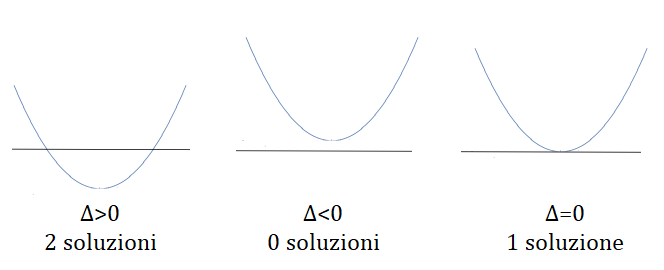
\includegraphics[width=.9\textwidth]{immagini/cap_4/fig_4_1.png}
\end{center}
\end{figure}
Pertanto
\begin{equation}
\langle i \left[R,S \right] \rangle ^2 - 4\langle R^2 \rangle \langle S^2 \rangle \leq 0,
\end{equation}
ossia
\begin{equation}
\langle R^2 \rangle \langle S^2 \rangle \geq \frac{1}{4}\langle i \left[R,S \right] \rangle ^2.
\end{equation}
Scegliendo infine $R=\Delta A$ ed $S= \Delta B$ si ottiene la relazione di indeterminazione \eqref{eq:cap4_2}.
\section[Esempio: autovalori ed autovettori dello spin per particelle di spin 1/2 e relazioni di indeterminazione]{Esempio: autovalori ed autovettori dello spin per\\ particelle di spin 1/2 e relazioni di indeterminazione}
Consideriamo nuovamente un sistema costituito da particelle di spin 1/2. Abbiamo già visto che i corrispondenti stati di singola particella possono essere espressi come combinazione lineare di sue stati di base, che qui indichiamo con $\vert +z\rangle $ e $\vert - z \rangle$, che rappresentano gli stati in cui la proiezione dello spin della particella lungo l'asse $z$ vale rispettivamente $S_z = \pm \hbar /2$. È evidente che in questa base l'operatore $S_z$ è rappresentato dalla seguente matrice:
\begin{equation}
S_z = \left( 
\begin{array}{cc}
\langle +z \vert S_z \vert +z \rangle &  \langle +z \vert S_z \vert -z \rangle \\
\langle -z \vert S_z \vert +z \rangle & \langle -z \vert S_z \vert -z \rangle  
\end{array}
\right)= \frac{\hbar}{2}\begin{pmatrix}
1 & 0 \\
0 & -1
\end{pmatrix}
\end{equation}
o, equivalentemente
\begin{equation}
S_Z =\frac{\hbar}{2}\sigma _z,
\end{equation}
dove $\sigma _z$ è la matrice di Pauli.\\
Utilizzando le proprietà generali dell'operatore di spin è possibile anche dimostrare che per gli analoghi operatori di $S_x$ ed $S_y$ valgano le corrispondenti rappresentazioni:
\begin{eqnarray}
& &\displaystyle{S_x = \frac{\hbar}{2}\sigma _x= \frac{\hbar}{2}\begin{pmatrix}
0 & 1 \\
1 & 0
\end{pmatrix}
} \\
\nonumber \\
& &\displaystyle{S_y= \frac{\hbar}{2}\sigma _y = \frac{\hbar}{2} \begin{pmatrix}
0 & -i \\
i & 0
\end{pmatrix}}
\end{eqnarray}
Poiché le tre matrici di Pauli hanno determinante uguale a $-1$ e traccia nulla, i loro autovalori sono $+1$ o $-1$. Corrispondentemente, gli autovalori della proiezione dello spin lungo un qualunque asse sono $\pm \hbar/2$. È immediato calcolare i corrispondenti autovettori:
\begin{eqnarray}
\label{eq:cap4_4}
& &\displaystyle{S_x = \frac{\hbar}{2}, \quad \vert x \rangle = \frac{1}{\sqrt{2}}\vert +z \rangle + \frac{1}{\sqrt{2}}\vert -z \rangle}= \frac{1}{\sqrt{2}}
\begin{pmatrix}
1\\
1
\end{pmatrix} \nonumber \\
\\
& &\displaystyle{S_x = -\frac{\hbar}{2}, \quad \vert -x \rangle = \frac{1}{\sqrt{2}}\vert +z \rangle - \frac{1}{\sqrt{2}}\vert -z \rangle}= \frac{1}{\sqrt{2}} \begin{pmatrix}
1\\
-1
\end{pmatrix}\nonumber
\end{eqnarray}
\begin{eqnarray}
\label{eq:cap4_5}
& &\displaystyle{S_y = \frac{\hbar}{2}, \quad \vert y \rangle = \frac{1}{\sqrt{2}}\vert +z \rangle + \frac{i}{\sqrt{2}}\vert -z \rangle}= \frac{1}{\sqrt{2}} 
\begin{pmatrix}
1\\
i
\end{pmatrix} \nonumber \\
\\
& &\displaystyle{S_y = -\frac{\hbar}{2}, \quad \vert -y \rangle = \frac{1}{\sqrt{2}}\vert +z \rangle - \frac{i}{\sqrt{2}}\vert -z \rangle}= \frac{1}{\sqrt{2}} 
\begin{pmatrix}
1\\
-i
\end{pmatrix}\nonumber
\end{eqnarray}
\begin{center}
\fbox{\begin{minipage}{.9\textwidth}
Calcoliamo esplicitamente l'autostato di $\vert +x\rangle$ di $S_x$ con autovalore $+\hbar /2$. Scriviamo questo stato come combinazione lineare generica di autostati di $S_z$:
\begin{equation}
\vert +x \rangle = c_1\vert +z \rangle+ c_2\vert -z \rangle \doteq 
\begin{pmatrix}
c_1 \\
c_2
\end{pmatrix}
\end{equation}
Applicando l'equazione agli autovalori $S_x \vert+x\rangle =\hbar /2 \vert +x\rangle $ si ottiene:
\begin{equation}
\frac{\hbar}{2}
\begin{pmatrix}
0 & 1 \\
1 & 0
\end{pmatrix}
\begin{pmatrix}
c_1 \\
c_2
\end{pmatrix} =
\frac{h}{2}
\begin{pmatrix}
c_1 \\
c_2
\end{pmatrix}
\quad \Rightarrow \quad
\begin{cases}
c_2=c_1\\
c_1=c_2
\end{cases}
\end{equation}
La condizione di normalizzazione dello stato implica:
\begin{equation}
\langle +x \vert +x \rangle = \left( c_1 ^*\ c_2 ^*\right)\begin{pmatrix}
c_1\\c_2
\end{pmatrix} = \vert c_1 \vert ^2 +\vert c_2 \vert ^2 =1, 
\end{equation}
che, unitamente alla condizione $c_1=c_2$ implica $\vert c_1 =1/\sqrt{2}$. Possiamo allora scrivere:
\begin{equation}
c_1 =c_2 = \frac{e^{i\delta}}{\sqrt{2}}\ \Rightarrow \ \vert +x \rangle \frac{e^{i\delta}}{\sqrt{2}} \left(\vert +z \rangle + \vert -z \rangle \right).
\end{equation}
Il fattore di fase moltiplicativo, nel vettore di stato, è completamente arbitrario, ossia non interviene mai nelle quantità fisiche che sono la probabilità ($\vert \langle \alpha \vert +x \rangle \vert ^2$) ed i valori di aspettazione ($\langle +x \vert A \vert +x \rangle $). Una scelta possibile è 	quella effettuata effettuata in eq. \eqref{eq:cap4_4}, ossia $e^{i\delta}=1$.
\end{minipage}}
\end{center}
È semplice verificare questi risultati. Ad esempio si ha:
\begin{equation}
S_y \vert - y \rangle = \frac{\hbar}{2\sqrt{2}}\begin{pmatrix}
0 & -i\\
i & 0
\end{pmatrix}
\begin{pmatrix}
1\\-i
\end{pmatrix} = \frac{\hbar}{2\sqrt{2}} 
\begin{pmatrix}
-1 \\ i
\end{pmatrix} = -\frac{\hbar}{2} \vert -y \rangle .
\end{equation}
Gli operatori corrispondenti alle proiezioni dello spin lungo i tre assi non commutano tra loro. Per esempio, un calcolo esplicito del commutatore di $S_x$ ed $S_y$ conduce a:
\begin{eqnarray}
\left[ S_x , S_y \right] & = & S_x S_y-S_y S_x= \nonumber \\
& = &\frac{\hbar ^2}{4} \left[\begin{pmatrix}
0 & 1\\
1 & 0
\end{pmatrix} \begin{pmatrix}
0 & -i\\
i & 0
\end{pmatrix}- \begin{pmatrix}
0 & -i\\
i & 0
\end{pmatrix}\begin{pmatrix}
0 & 1\\
1 & 0
\end{pmatrix}
\right] = \\
& = &\frac{\hbar ^2}{4} \left[\begin{pmatrix}
i & 0\\
0 & -i
\end{pmatrix} - \begin{pmatrix}
-i & 0\\
0 & i
\end{pmatrix}\right] = \nonumber \\
& = & \frac{\hbar ^2}{2}\begin{pmatrix}
i & 0\\
0 & -i
\end{pmatrix}\nonumber
\end{eqnarray}
ossia
\begin{equation}
\left[ S_x, S_y \right] = i \hbar S_z.
\end{equation}
In generale, è possibile verificare che le tre relazioni di commutazione indipendenti possono essere scritte nella forma compatta
\begin{equation}
\left[ S_i , S_j\right] = i\ \varepsilon_{ijk}\ \hbar S_k,
\end{equation}
dove gli indici 1,2,3 sono associati rispettivamente alle componenti $x$, $y$ e $z$.\\
Le relazioni di commutazione qui derivate implicano che \textbf{le componenti dello spin lungo assi distinti non possono essere misurate simultaneamente, ossia che queste tre grandezze fisiche sono osservabili incompatibili}. Corrispondentemente, deve risultare soddisfatta una \textbf{relazione di indeterminazione}. Nel caso della misura di $S_x$ ed $S_y$, per esempio, questa relazione assume la forma
\begin{equation}
\label{eq:cap4_6}
\langle (\Delta S_x) ^2 \rangle \langle (\Delta S_y) ^2 \rangle \geq \frac{1}{4} \vert \langle \left[ S_x , S_y \right] \rangle \vert ^2 = \frac{\hbar}{4} \langle S_z \rangle ^2 .
\end{equation}
Verifichiamo la validità di questa relazione per una particella che si trovi ad esempio nello stato $\vert +z\rangle$. In generale, lo scarto quadratico medio di una grandezza $A$ si esprime come
\begin{eqnarray}
\langle (\Delta A ) ^2 \rangle & = & \langle (A- \langle A \rangle ) ^2 \rangle = \langle (A^2-2A\langle A \rangle + \langle A \rangle ^2) \rangle = \nonumber \\
\\
& = & \langle A^2\rangle - \langle A \rangle ^2, \nonumber
\end{eqnarray}
e dipende dunque dai valori medi di $A$ e $A^2$.\\
Nel caso di $(\Delta S_x) ^2$, allora, calcoliamo in primo luogo l'operatore $S_x ^2$:
\begin{equation}
S_x ^2 = \frac{\hbar ^2}{4} \sigma _x ^2=\frac{\hbar ^2}{4} \begin{pmatrix}
0 & 1 \\
1 & 0
\end{pmatrix} \begin{pmatrix}
0 & 1 \\
1 & 0
\end{pmatrix} = \frac{\hbar ^2}{4}\begin{pmatrix}
1 & 0 \\
0 & 1
\end{pmatrix}.
\end{equation}
(Osserviamo che le matrici di Pauli soddisfano $\sigma _x ^2 = \sigma _y ^2 = \sigma _z ^2 =1$).\\
Poiché lo stato $\vert +z \rangle$, su cui vogliamo verifica la relazione di indeterminazione, è uno degli stati di base, i valori medi di $S_x$ ed $S_x ^2$ su questo stato si ottengono direttamente dai corrispondenti elementi di matrice (elementi 1,1):
\begin{eqnarray}
& &\displaystyle{\langle +z \vert S_x \vert +z \rangle = (S_x)_{11} = \frac{\hbar}{2}\cdot 0 =0}  \nonumber \\
\\
& &\displaystyle{\langle +z \vert S_x ^2\vert +z \rangle = (S_x ^2)_{11} = \frac{\hbar ^2}{4}\cdot 1 =\frac{\hbar ^2}{4}} \nonumber
\end{eqnarray}
Ne segue allora
\begin{equation}
\label{eq:cap4_7}
\langle +z \vert (\Delta S_x)^2\vert +z \rangle = \frac{\hbar ^2}{4}.
\end{equation}
Analogamente si calcola $\langle (\Delta S_y)^2 \rangle $ ($S_y ^2= \frac{\hbar ^2}{4}\cdot I$):
\begin{eqnarray}
& &\displaystyle{\langle +z \vert S_y \vert +z \rangle = (S_y)_{11} = \frac{\hbar}{2}\cdot 0 =0}  \nonumber \\
\\
& &\displaystyle{\langle +z \vert S_y ^2\vert +z \rangle = (S_y ^2)_{11} = \frac{\hbar ^2}{4}\cdot 1 =\frac{\hbar ^2}{4}} \nonumber
\end{eqnarray}
da cui
\begin{equation}
\label{eq:cap4_8}
\langle +z \vert (\Delta S_y)^2\vert +z \rangle = \frac{\hbar ^2}{4}.
\end{equation}
Il secondo membro della relazione di indeterminazione è in questo caso, a parte il fattore $\frac{\hbar ^2}{4}$, semplicemente il valore medio di $S_z$ al quadrato:
\begin{equation}
\label{eq:cap4_9}
\left( \langle +z \vert S_z \vert +z \rangle \right) ^2 = \frac{\hbar ^2}{4}.
\end{equation}
Mettendo insieme i risultati \eqref{eq:cap4_7}, \eqref{eq:cap4_8} e \eqref{eq:cap4_9} possiamo allora verificare esplicitamente la relazione di indeterminazione \eqref{eq:cap4_6}:
\begin{equation}
\langle  (\Delta S_x)^2 \rangle \langle(\Delta S_y)^2 \rangle = \left(\frac{\hbar ^2}{4} \right) ^2 \geq \frac{\hbar ^2}{4} \langle S_z  \rangle ^2 = \left(\frac{\hbar ^2}{4} \right) ^2.
\end{equation}
La relazione di indeterminazione risulta quindi soddisfatta, in questo caso, con il segno di uguaglianza. In altri termini, sullo stato $\vert +z \rangle $ il prodotto delle indeterminazioni su $S_x$ e $S_y$ assume il valore minimo possibile compatibilmente con la relazione di indeterminazione.\\ \\
\textbf{Appendice:}\\
Vediamo come, considerando ad esempio lo stato $\vert + z \rangle $, i valori medi $\langle S_x \rangle $ e $\langle (\Delta S_x)^2 \rangle $ possano essere calcolai anche utilizzando la definizione di valore medio:
\begin{equation}
\langle A \rangle = \sum _i a_i p_i,
\end{equation}
dove $A_I$ sono i possibili risultati della misura di $A$ e $p_i$ le corrispondenti probabilità.\\
Utilizzando le eq.\eqref{eq:cap4_7} è semplice trovare che lo stato $\vert +z \rangle$ si esprime come combinazione lineare degli autostati si $S_x$ nella forma
\begin{equation}
\vert +z \rangle = \frac{1}{\sqrt{2}} \vert +x \rangle + \frac{1}{\sqrt{2}} \vert -x \rangle .
\end{equation}
I possibili risultati di una misura di $S_x$ e le corrispondenti probabilità su questo stato sono allora
\begin{equation}
\begin{cases}
\displaystyle{S_x ^{(1)} = +\frac{\hbar}{2}, \ p_1 = \frac{1}{2}} \\
\\
\displaystyle{S_x ^{(2)} = -\frac{\hbar}{2}, \ p_2 = \frac{1}{2}}
\end{cases}
\end{equation}
Per i valori medi si $S_x$ si ottiene allora:
\begin{equation}
\langle S_x \rangle = \sum _i S_x ^{(i)} p_i= +\frac{\hbar}{2}\cdot\frac{1}{2}-\frac{\hbar}{2}\cdot\frac{1}{2}=0,
\end{equation}
mentre per lo scarto quadratico medio
\begin{equation}
\langle (\Delta S_x)^2 \rangle = \sum _i ( S_x ^{(i)}- \underbrace{\langle S_x \rangle}_{=0}) ^2\ p_i= +\frac{\hbar ^2}{4}\cdot\frac{1}{2}+\frac{\hbar ^2}{4}\cdot\frac{1}{2}= \frac{\hbar ^2}{2},
\end{equation}
in accordo con i precedenti risultati ottenuti.%DEFINITIVO
\chapter[Autostati dell'operatore di posizione]{Autostati dell'operatore di posizione, misure di posizione e funzione d'onda\footnote{S1.6,1.7}}
Abbiamo assunto che le osservabili finora considerate abbiano uno spettro discreto di autovalori. In meccanica quantistica, tuttavia, vi sono \textbf{osservabili con autovalori continui}.\\
Un caso particolarmente importante di osservabile con spettro continuo è rappresentato dalla \textbf{posizione}.
Consideriamo (per semplicità) una particella vincolata a muoversi in una dimensione e sia $x$ l'asse lungo il quale è possibile il moto. Possiamo allora pensare di indicare con il simbolo $\ket{x'}$ \textbf{lo stato in cui la particella si trova nella posizione x}.
Una misura di posizione per una particella che si trovi nello spazio $\ket{x'}$ fornisce (per definizione) con certezza il valore $x'$. In altri termini, lo stato $\ket{x'}$ deve essere un \textbf{autostato dell'operatore di posizione} corrispondente all'autovalore $x'$.
\begin{equation}
  x\ket{x'} = x'\ket{x'} .
\end{equation}
In questa equazione $x'$ è semplicemente un numero mentre $x$ rappresenta \textbf{l'operatore posizione}.
Così come uno stato qualsiasi può essere sviluppato in serie di autostati di una grandezza con spettro discreto, allo stesso modo \textbf{uno stato può essere sviluppato}, questa volta in integrale, \textbf{secondo un sistema completo di autostati di una grandezza con spettro continuo}. Nel caso degli autostati dell'operatore posizione, questo sviluppo ha la forma
\begin{equation}
  \label{eq:cap5_1}
  \ket{\alpha} = \int_{-\infty}^{\infty}\dd{x'}\ket{x'}\braket{x'}{\alpha} .
\end{equation}
Contrariamente al caso di variabili con spettro discreto, il modulo quadro $\abs{\braket{x'}{\alpha}}^2$ non può essere interpretato come probabilità che una particella nello stato $\ket{\alpha}$ venga a trovarsi nella posizione $x'$. Infatti, per una variabile continua, tale probabilità è nulla.\\
Il significato fisico dell'ampiezza $\braket{x'}{\alpha}$ può essere derivato nel modo seguente.
Utilizzando lo sviluppo (\ref{eq:cap5_1}) calcoliamo il valore medio della posizione nello stato $\ket{\alpha}$
\begin{align}
  \ev{x}{\alpha} = \int_{-\infty}^{\infty}\dd{x'}\mel{\alpha}{x}{x'}\braket{x'}{\alpha}=\int_{-\infty}^{\infty}\dd{x'}x'\abs{\braket{x'}{\alpha}}^2 .
\end{align}
Da questa espressione vediamo che la quantità
\begin{equation}
  \abs{\braket{x'}{\alpha}}^2\dd x'
\end{equation}
rappresenta la probabilità che la particella nello stato $\ket{\alpha}$ si trovi posizionata in un intervallo di larghezza $\dd{x'}$ attorno al punto $x'$.\\
Per un intervallo infinitesimo, \textbf{la probabilità che una particella nello stato }$\ket{\alpha}$ \textbf{si trovi compresa in un intervallo di larghezza }$\dd{x'}$ \textbf{nell'intorno del punto }$x'$ \textbf{è}:
\begin{equation}
  P\qty(x'-\frac{\dd{x'}}{2}, x'+\frac{\dd{x'}}{2}) = \abs{\braket{x'}{\alpha}}^2\dd{x'} .
\end{equation}
Dall'equazione (\ref{eq:cap5_1}) risulta che questa probabilità è correttamente normalizzata
La probabilità di registrare la particella in qualche punto compreso tra $-\infty$ e $+\infty$ è data da $\int_{-\infty}^{+\infty}\dd{x'}\abs{\braket{x'}{\alpha}}^2$.
Dall'equazione (\ref{eq:cap5_1}) risulta che questa probabilità è correttamente normalizzata all'unità se lo stato $\ket{\alpha}$ è normalizzato:
\begin{equation}
  \label{eq:cap5_2}
  \int_{-\infty}^{+\infty}\dd{x'}\abs{\braket{x'}{\alpha}}^2 = \int_{-\infty}^{+\infty}\dd{x'}\braket{\alpha}{x'}\braket{x'}{\alpha}=\braket{\alpha}{\alpha} = 1 .
\end{equation}
Solitamente il prodotto scalare $\braket{x'}{\alpha}$ prende la denominazione di \textbf{funzione d'onda} $\psi_{\alpha}\qty(x')$ per lo stato $\ket{\alpha}$
\begin{equation}
  \braket{x'}{\alpha} = \psi_{\alpha}\qty(x')
\end{equation}
L'equazione (\ref{eq:cap5_2}) esprime la \textbf{condizione di normalizzazione per la funzione d'onda}
\begin{equation}
  \int_{\infty}^{+\infty}\dd{x'}\abs{\psi_{\alpha}\qty(x')}^2=1 .
\end{equation}
Utilizzando l'equazione (\ref{eq:cap5_1}), che definisce la relazione di completezza degli autostati della posizione, \textbf{è possibile esprimere una qualunque ampiezza} $\braket{\beta}{\alpha}$ \textbf{in termini di un integrale di sovrapposizione delle funzioni d'onda per gli stati} $\ket{\beta}$ \textbf{ed} $\ket{\alpha}$:
\begin{equation}
  \int_{\infty}^{+\infty}\dd{x'}\braket{\beta}{x'}\braket{x'}{\alpha} = \int_{\infty}^{+\infty}\dd{x'} \psi^*_{\beta}\qty(x')\psi_{\alpha}\qty(x') .
\end{equation}
Similmente, lo sviluppo di un vettore di stato $\ket{\alpha}$ in autostati di un osservabile con spettro discreto $A$,
\begin{equation}
  \ket{\alpha} = \sum_{a'}\ket{a'}\braket{a'}{\alpha}\equiv \sum_{a'}C_{a'}\ket{a'} ,
\end{equation}
può essere espresso in termini di uno \textbf{sviluppo della funzione d'onda} $\psi_{\alpha}$ \textbf{in "autofunzioni" dell'operatore $A$}.
Moltiplicando la precedente equazione a sinistra per il bra $\bra{x'}$ si ottiene infatti:
\begin{equation}
  \psi_{\alpha}\qty(x') = \sum_{a'}C_{a'}u_{a'}\qty(x') ,
\end{equation}
dove si sono introdotte le \textbf{autofunzioni} dell'operatore $A$ corrispondenti agli autovalori $a'$:
\begin{equation}
  u_{a'}\qty(x') = \braket{x'}{a'} .
\end{equation}
\section[Normalizzazione degli autostati dell'operatore di posizione e funzione Delta di Dirac]{Normalizzazione degli autostati dell'operatore di posizione e funzione Delta di Dirac\footnote{ S1.6,1.7,LL5}}
Più complessa che nel caso dello spettro discreto è la questione della \textbf{normalizzazione degli autostati di osservabili con spettro continuo}
 ed in particolare, dunque, dell'operatore di posizione.
 Per dedurre la condizione di normalizzazione moltiplichiamo a sinistra l'equazione (\ref{eq:cap5_1}) per un autostato della posizione:
 \begin{equation}
   \label{eq:cap5_3}
   \braket{x'}{\alpha} = \int_{-\infty}^{+\infty}\dd{x''}\braket{x'}{x''}\braket{x''}{\alpha} .
 \end{equation}
Questa equazione deve valere per $\braket{x'}{\alpha}$ arbitrari e deve quindi essere un'identità. A tale scopo è necessario, anzitutto, che il coefficiente di $\braket{x''}{\alpha}$, cioè l'ampiezza $\braket{x'}{x''}$ si annulli per tutti gli $x'\neq x''$. Per $x'=x''$, questa ampiezza deve diventare infinita; viceversa l'integrale in $\dd{x''}$ semplicemente nullo. In tal modo, l'ampiezza $\braket{x'}{x''}$ è una funzione della differenza $x'-x''$, che si annulla allorché questa differenza è diversa da zero e diventa infinita allorché questa è nulla. Indichiamo questa funzione con $\delta\qty(x'-x'')$
\begin{equation}
  \braket{x'}{x''} = \delta\qty(x'-x'') .
\end{equation}
Il modo in cui la funzione $\delta\qty(x'-x'')$ diventa infinita per $x'-x''=0$ è determinato dall'equazione (\ref{eq:cap5_3}) che possiamo scrivere in forma generale come
\begin{equation}
  f\qty(x_0) = \int_{-\infty}^{+\infty}\dd{x}\delta\qty(x-x_0)f\qty(x) .
\end{equation}
È ovvio che a questo scopo si deve avere in particolare
\begin{equation}
  \int_{-\infty}^{+\infty}\dd{x}\delta\qty(x-x_0) = 1 .
\end{equation}
La funzione così definita si chiama \textbf{funzione $\delta$ di Dirac}.
Riepiloghiamo le formule che la definiscono
\begin{align}
  \delta(x) = 0 \quad \text{per }x\neq 0 ; \\
  \delta(0) = \infty ; \\
  \int_{-\infty}^{+\infty}\dd{x}\delta(x)=1 .
\end{align}
È ovvio che come limiti di integrazione nell'ultima equazione si possono prendere due altri valori qualsiasi tra cui è compreso il punto $x=0$.
Presentiamo qui alcune possibili definizioni della $\delta$ di Dirac come limite di funzioni ordinarie
\begin{itemize}
\item
\begin{tabular}{ >{\centering\arraybackslash} m{1.5cm} >{\centering\arraybackslash} m{3.5cm} >{\centering\arraybackslash} m{4.5cm}}
$\displaystyle{\lim _{a \rightarrow 0}}$ & 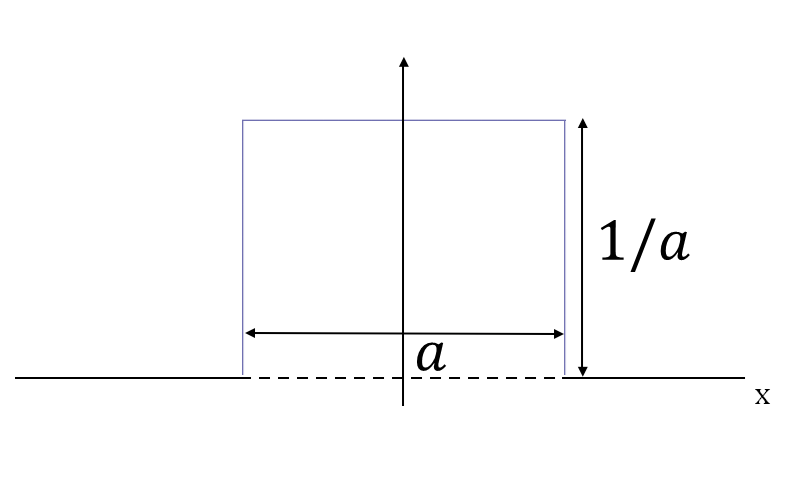
\includegraphics[width=3.5cm]{immagini/cap_5/fig_5_1.png}  & $=\displaystyle{\begin{cases}
1/a \textrm{ per } \vert x \vert \leq a/2\\
0 \textrm{ per } \vert x \vert > a/2
\end{cases}}$
\end{tabular}
\item
\begin{tabular}{ >{\centering\arraybackslash} m{4cm} >{\centering\arraybackslash} m{3.5cm} >{\centering\arraybackslash} m{2cm}}
$\displaystyle{\lim _{a \rightarrow 0}\frac{1}{a\sqrt{\pi}}e^{-x^2/a^2}=}$ & 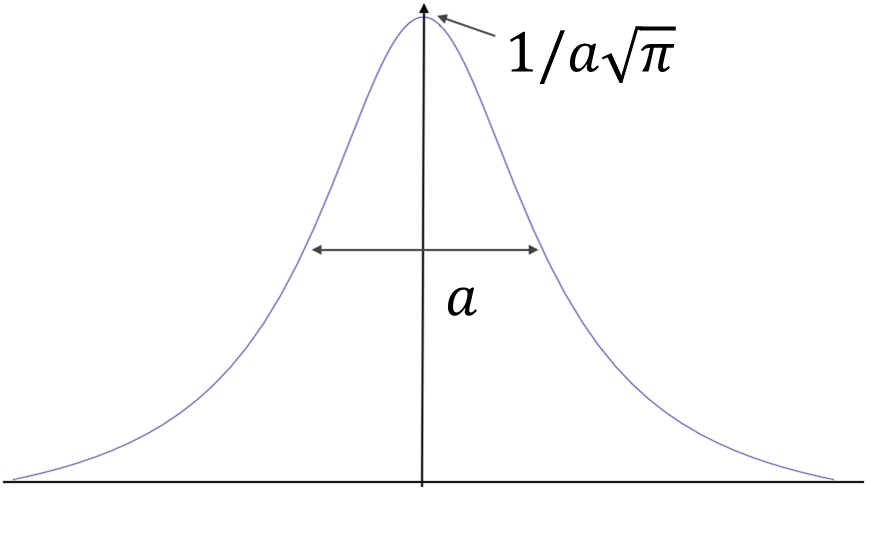
\includegraphics[width=3.5cm]{immagini/cap_5/fig_5_2.png}  & (gaussiana)
\end{tabular}
\item 
\begin{tabular}{ >{\centering\arraybackslash} m{4cm} >{\centering\arraybackslash} m{3.5cm} >{\centering\arraybackslash} m{2cm}}
$\displaystyle{\lim _{a \rightarrow 0}\frac{1}{\pi}\frac{a^2}{x^2+a^2}}=$ & 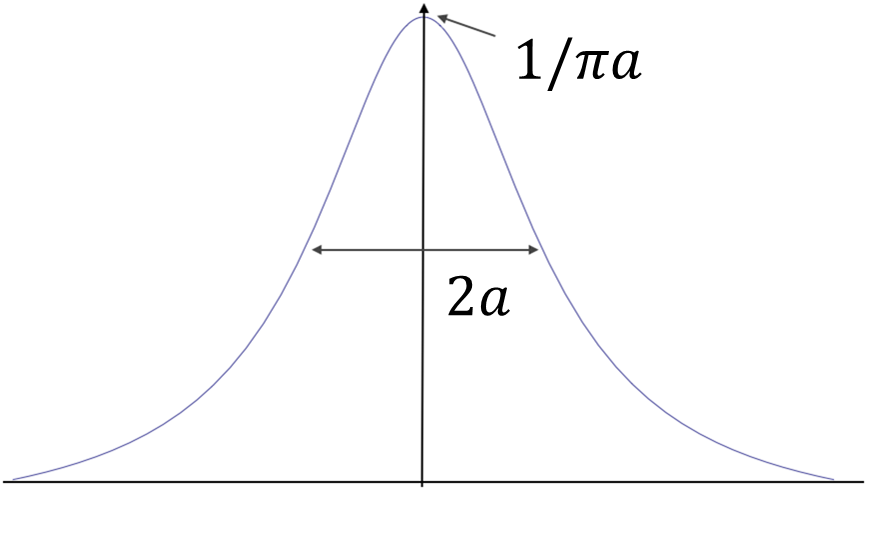
\includegraphics[width=3.5cm]{immagini/cap_5/fig_5_3.png}  & (lorentziana)
\end{tabular}
\item 
\begin{tabular}{ >{\centering\arraybackslash} m{4cm} >{\centering\arraybackslash} m{3.5cm} >{\centering\arraybackslash} m{2cm}}
$\displaystyle{\lim _{a \rightarrow 0}\frac{\sin(x/a)}{\pi x}}=$ & 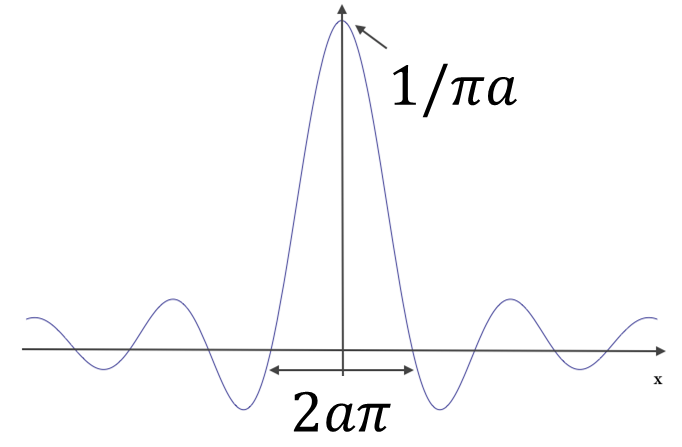
\includegraphics[width=3.5cm]{immagini/cap_5/fig_5_4.png}  & 
\end{tabular}
\end{itemize}
Dall'ultima definizione segue anche la rappresentazione integrale della $\delta$ di Dirac:
\begin{equation}
  \delta\qty(x) = \lim_{a\to0}\frac{\sin{x/a}}{\pi x}=\lim_{a\to0}\frac{1}{2\pi}\int_{-\frac{1}{a}}^{\frac{1}{a}}\dd{k}e^{ikx} ,
\end{equation}
ossia
\begin{equation}
  \delta(x)=\frac{1}{2\pi}\int_{-\infty}^{\infty}\dd{x}e^{ikx} .
\end{equation}
\section{Operatori nella rappresentazione delle coordinate}
In precedenza abbiamo discusso come una qualsiasi ampiezza $\braket{\beta}{\alpha}$ possa esprimersi in termini di un integrale di sovrapposizione delle funzione d'onda $\psi_{\beta}$ e $\psi_{\alpha}$ degli stati $\ket{\beta}$ e $\ket{\alpha}$.
Esaminiamo ora come gli \textbf{elementi di matrice} $\mel{\beta}{A}{\alpha}$ possano essere scritti usando le funzioni d'onda $\psi_{\beta}$ e $\psi_{\alpha}$. Si ha evidentemente:
\begin{align}
  \label{eq:cap5_4}
  \mel{\beta}{A}{\alpha} &= \int\dd{x'}\int\dd{x''}\braket{\beta}{x'}\mel{x'}{A}{x''}\braket{x''}{\alpha} =\nonumber\\
  &= \int\dd{x'}\int\dd{x''} \psi_{\beta}^*\qty(x')\mel{x'}{A}{x''}\psi_{\alpha}\qty(x'') .
\end{align}
L'ampiezza $\mel{\beta}{A}{\alpha}$ è dunque completamente determinata in termini di un integrale contenente le funzioni d'onda $\psi_{\beta}$ e $\psi_{\alpha}$ e gli elementi di matrice $\mel{x'}{A}{x''}$. Questi sono detti \textbf{elementi di matrice dell'operatore $A$ nella rappresentazione delle coordinate e sono, in generale, una funzione delle due variabili $x'$ e $x''$}.
Una notevole semplificazione si ha quando l'osservabile $A$ è una funzione dell'operatore posizione $X$. Consideriamo per esempio il caso in cui
\begin{equation}
  A= x^2 .
\end{equation}
Abbiamo allora:
\begin{equation}
  \mel{x'}{x^2}{x''} = \bra{x'}\qty(x''^2\ket{x''}) = x''^2\delta\qty(x'-x'') = x'^2\delta\qty(x'-x'') ,
\end{equation}
dove si è usato il fatto che $\ket{x''}$ è un autostato dell'operatore $x$ corrispondente all'autovalore $x''$ e la condizione di normalizzazione degli autostati di posizione. Sostituendo questo risultato nell'equazione (\ref{eq:cap5_4}) l'integrale doppio si riduce ad un integrale semplice in virtù delle proprietà della funzione $\delta$:
\begin{align}
  \mel{\beta}{x^2}{\alpha} &=\int\dd{x'}\int\dd{x''} \psi_{\beta}^*\qty(x')x'^2\delta\qty(x'-x'')\psi_{\alpha}\qty(x'') =\nonumber\\
  &= \int\psi_{\beta}^*\qty(x')x'^2\psi_{\alpha}\qty(x') .
\end{align}
In generale per un operatore funzione del solo operatore posizione $x$ si ha:
\begin{equation}
  \mel{\beta}{f(x)}{\alpha} = \int\dd{x'}\psi_{\beta}^*\qty(x')f\qty(x')\psi_{\alpha}\qty(x') .
\end{equation}
Si noti che $f(x)$ primo membro di queste equazioni è un operatore, mentre $f\qty(x')$ nel secondo membro non è un operatore.
\section[Regole di commutazione per gli operatori di posizione]{Regole di commutazione per gli operatori di posizione \footnote{S1.6}}
Le proprietà dell'operatore posizione sin qui considerate possono essere facilmente generalizzate al caso di tre dimensioni spaziali.
Possiamo indicare con il simbolo $\ket{\va{x}'}$ \textbf{il vettore di stato di una particella che si trovi nel punto di coordinate $\va{x}'= \qty(x',y',z')$}.
Una misura di posizione per una particella che si trovi nello stato $\ket{\va{x}'}$ fornisce con certezza i valori $x'$, $y'$ e $z'$ per le tre coordinate spaziali rispettivamente. In altri termini il vettore di stato $\ket{\va{x}'}$ è autostato simultaneo delle osservabili $x$, $y$ e $z$:
\begin{equation}
  x\ket{\va{x}'}=x'\ket{\va{x}'},\quad y\ket{\va{x}'}=y'\ket{\va{x}'},\quad z\ket{\va{x}'}=z'\ket{\va{x}'} .
\end{equation}
Sappiamo che per poter considerare un autostato simultaneo di $x$, $y$, e $z$ dobbiamo assumere che le tre componenti del vettore posizione possano essere misurate simultaneamente con un grado di precisione arbitrario. Dobbiamo perciò avere
\begin{equation}
  \comm{x_i}{x_j}= 0 ,
\end{equation}
dove $x_1$, $x_2$ ed $x_3$ stanno per $x$, $y$ e $z$ rispettivamente.%DEFINITIVO
\chapter{Richiami di Meccanica Classica}
\section[Parentesi di Poisson]{Parentesi di Poisson\footnote{LL, Meccanica, \S 42}}
Sia $f(\mathbf{p},\mathbf{q},t)$ una funzione delle coordinate degli impulsi e del tempo e calcoliamone la sua derivata totale rispetto al tempo:
\begin{equation}
\frac{df}{dt}= \frac{\partial f}{\partial t} + \sum_i \left( \frac{\partial f}{\partial q_i} \dot {q_i} + \frac{\partial f}{\partial p_i} \dot {p_i} \right).
\end{equation}
Utilizzando le equazioni di Hamilton:
\begin{equation}
\dot{q_i}=\frac{\partial H}{\partial p_i} , \qquad \dot{p_i}=-\frac{\partial H}{\partial q_i} ,
\end{equation}
possiamo scrivere:
\begin{equation}
\frac{df}{dt}=	\frac{\partial f}{\partial t} + \sum_i \left( \frac{\partial H}{\partial p_i}\frac{\partial f}{\partial q_i}-\frac{\partial H}{\partial q_i}\frac{\partial f}{\partial p_i}\right) \equiv \frac{\partial f}{\partial t} + \left\lbrace H,f \right\rbrace ,
\end{equation}
dove si \`e introdotta la notazione:
\begin{equation}
\left\lbrace H,f \right\rbrace \equiv \sum_i \left(\frac{\partial H}{\partial p_i}\frac{\partial f}{\partial q_i}-\frac{\partial H}{\partial q_i}\frac{\partial f}{\partial p_i}\right)  .
\end{equation}.
La quantit\`a $\left\lbrace H,f \right\rbrace$ è detta \textbf{parentesi di Poisson} di $H$ con $f$. In generale:
\begin{equation}
\left\lbrace f,g \right\rbrace \equiv \sum_i \left(\frac{\partial f}{\partial p_i}\frac{\partial g}{\partial q_i}-\frac{\partial f}{\partial q_i}\frac{\partial g}{\partial p_i}\right)  .
\end{equation}.
Se $f(\mathbf{p},\mathbf{q},t)$ \`e una costante del moto, allora
\begin{equation}
\frac{\partial f}{\partial t}+\left\lbrace H,f \right\rbrace   \equiv 0 , \qquad
\left( \frac{df}{dt}=0 \right) .
\end{equation}.
Se l'integrale del moto non dipende esplicitamente dal tempo, allora
\begin{equation}
\left\lbrace H,f \right\rbrace  \equiv 0 ,
\end{equation}
ossia la sua parentesi di Poisson con l'Hamiltoniana deve annullarsi.\\
Come esempio specifico consideriamo il caso in cui la funzione $f$ \`e la stessa Hamiltoniana $H$ del sistema. Si ha
\begin{equation}
\frac{d H}{d t} = \frac{\partial H}{\partial t} + \left\lbrace H,H \right\rbrace = \frac{\partial H}{\partial t}
\end{equation}
Per un sistema isolato, l'Hamiltoniana $H$, in virt\`u dell'omogeneit\`a del tempo, non dipende esplicitamente dal tempo: $\partial H/ \partial t=0$ In questo caso risulta allora
\begin{equation}
\frac{d H}{d t} = 0 \qquad \textrm{sui sistemi isolati,}
\end{equation}
che esprime la legge di conservazione dell'energia.
Consideriamo la parentesi di Poisson di una funzione $f$ con una componente delle coordinate e degli impulsi:
\begin{eqnarray}
\left\lbrace f,q_k \right\rbrace &=& \sum_i \left( \frac{\partial f}{\partial p_i} \frac{\partial q_k}{\partial q_i} - \frac{\partial f}{\partial q_i}\frac{\partial q_k}{\partial p_i} \right) = \frac{\partial f}{\partial p_k} ,\\
\nonumber \\
\left\lbrace f,p_k \right\rbrace &=& \sum_i \left( \frac{\partial f}{\partial p_i} \frac{\partial p_k}{\partial p_i} - \frac{\partial f}{\partial q_i}\frac{\partial p_k}{\partial p_i} \right) = - \frac{\partial f}{\partial q_k} .
\end{eqnarray}
Da queste segue allora anche:
\begin{equation}
\begin{matrix}
\left\lbrace q_i,q_k \right\rbrace =0 , &  \left\lbrace p_i,p_k \right\rbrace =0 , & \left\lbrace p_i,q_k \right\rbrace = \delta_{i,k} .
\end{matrix}
\end{equation}

\section[Trasformazioni Canoniche]{Trasformazioni Canoniche\footnote{LL, Meccanica, \S 45}}
Nel formalismo lagrangiano la scelta delle coordinate non \`e limitata da alcuna condizione: la loro funzione pu\`o essere determinata da $N$ grandezze qualsiasi che definiscono univocamente la posizione del sistema nello spazio. La forma delle equazioni di Lagrange non dipende da questa scelta. In altri termini, in luogo di un insieme di coordinate $q$ che soddisfano le equazioni:
\begin{equation}
\frac{d}{dt}  \left( \sum_i\frac{\partial L}{\partial \dot{q}_i} \right) - \sum_i \frac{\partial L}{\partial q_i} = 0 ,
\end{equation}
posso scegliere un differente insieme $Q$, dove in generale:
\begin{equation}
Q_i = Q_i(q,t) .
\label{eq:cap6_1}
\end{equation}
La nuova lagrangiana $L$ \`e definita dall'equazione
\begin{equation}
L'(Q,\dot{Q},t) = L'\left(Q(q,t), \dot {Q}(q, \dot{q}, t), t \right) = L(q,\dot{q},t) ,
\end{equation}
e valgono le equazioni di Eulero-Lagrange\footnote{DIM: Si utilizza $\dot{Q} = \frac{\partial Q}{\partial q}\dot{q} + \frac{\partial Q}{\partial t} \Rightarrow \frac{\partial \dot{Q}}{\partial \dot{q}} = \frac{\partial Q}{\partial q}$ }
\begin{equation}
\frac{d}{dt} \left( \sum_i \frac{\partial L}{\partial \dot{Q}_i} \right) - \frac{\partial L'}{\partial Q_i} = 0 .
\end{equation}
Queste trasformazioni lasciano inoltre evidentemente invariata anche la forma delle equazioni di Hamilton giacch\'e queste possono essere dedotte a partire dalle equazioni di Eulero-Lagrange.\\
Nel formalismo hamiltoniano, tuttavia, le coordinate e gli impulsi sono variabili indipendenti. \`E possibile allora considerare, in luogo delle trasformazioni (\ref{eq:cap6_1}), una classe di trasformazioni pi\`u ampia, della forma:
\begin{equation}
\begin{matrix}
Q_i = Qi(p,q,t),  & P_i = Pi(p,q,t) .
\end{matrix}
\label{eq:cap6_2}
\end{equation}.
La possibilit\`a di allargare la classe delle trasformazioni ammissibili rappresenta uno dei vantaggi sostanziali della formulazione hamiltoniana della meccanica.
In generale, tuttavia, trasformazioni della forma (\ref{eq:cap6_2}) non conducono ad equazioni di Hamilton nella forma canonica, ossia
\begin{equation}
\begin{matrix}
\dot{Q}_i = \frac{\partial H'}{\partial \mathbf{P}_i}, & \dot{P}_i = -\frac{\partial H'}{\partial \mathbf{Q}_i}  ,
\end{matrix}
\end{equation}
con una nuova $H'$.\\
La classe di trasformazioni (\ref{eq:cap6_2}) per le quali ci\`o invece accade sono dette \textit{trasformazioni canoniche}. Stabiliamo le condizioni per le quali le trasformazioni (\ref{eq:cap6_2}) risultano essere trasformazioni canoniche.
Poich\`e $ L = \sum _i p_i \dot{q}_i -H $, le equazioni di Hamilton possono essere derivate dal principio di minima azione scritto nella forma:
\begin{equation}
\partial S = \delta \int_{t_1}^{t_2} \left[ \sum_i p_i \dot{q}_i - H \right] dt = \delta \int \left[ \sum_i p_i dq_i - Hdt \right] = 0 .
\label{eq:cap6_3}
\end{equation}
Considerando le variazioni $p_i \rightarrow p_i + \delta p_i$ , $q_i \rightarrow q_i + \delta q_i$ si ha infatti:

\begin{eqnarray}
\delta S & =& \int _{t_1} ^{t_2} \sum _i \left[ \delta p_i \dot{q}_i + p_i \delta \dot{q}_i - \frac{\partial H}{\partial p_i} \delta p_i - \frac{\partial H}{\partial q_i}\delta q_i \right] dt = \nonumber \\
&=&\int _{t_1} ^{t_2} \sum _i \left[ \delta p_i \dot{q}_i + p_i \delta \dot{q}_i - \frac{\partial H}{\partial p_i} \delta p_i - \frac{\partial H }{\partial q_i} \delta q_i \right] dt + \left.\sum_i  p_i \delta q_i \right\vert _{t_1} ^{t_2} = \nonumber \\
&=& \int _{t_1} ^{t_2} \sum _i \left[ \left( \dot{q}_i - \frac{\partial H}{\partial p_i} \right) \delta p_i - \left( \dot{p}_i + \frac{\partial H}{\partial q_i}\right)\delta q_i \right] dt = 0 ,
\end{eqnarray}
da cui
\begin{equation}
\begin{matrix}
\dot{q}_i = \frac{\partial H}{\partial p_i} , & \dot{p}_i = - \frac{\partial H}{\partial q_i} .
\end{matrix}
\end{equation}
Se le nuove variabili $P_i$ e $Q_i$ sono definite da trasformazioni canoniche, ossia soddisfano le equazioni di Hamilton, allora devono soddisfare anche un principio di minima azione della forma:
\begin{equation}
\delta \int \left[ \sum_i P_i\ dQ_i - H'dt\right] = 0
\label{eq:cap6_4}
\end{equation}
Le eq. (\ref{eq:cap6_3}) e (\ref{eq:cap6_4}) possono risultare simultaneamente soddisfatte solo se le espressioni integrande differiscono al pi\`u per il differenziale totale di una funzione $F$ degli impulsi, delle coordinate e del tempo. In tal caso la differenza tra i due integrali, ossia la differenza dei valori della funzione $F$ nei limiti di integrazione, sar\`a una costante ininfluente ai fini della variazione. Si ha pertanto:
\begin{equation}
\sum_i p_i dq_i - Hdt = \sum_i P_i d Q_i - H'dt + dF .
\end{equation}.
Ogni trasformazione canonica \`e caratterizzata da una sua funzione $F$, detta \textit{funzione generatrice della trasformazione}.\\
Si ha pertanto:
Riscrivendo la precedente equazione nella forma
\begin{equation}
dF = \sum_i p_i d q_i - \sum_i P_i dQ_i + (H'-H)dt ,
\label{eq:cap6_5}
\end{equation}
vediamo che
\begin{equation}
\begin{matrix}
p_i = \frac{\partial F}{\partial q_i} , & P_i = - \frac{\partial F}{\partial Q_i} , & H' = H + \frac{\partial F}{\partial t} ,
\end{matrix}
\label{o}
\end{equation}
dove si \`e posto che la funzione generatrice \`e data come funzione delle vecchie e delle nuove coordinate del tempo:
\begin{equation}
F = F(q_i, Q_i,t) .
\end{equation}.
Pu\`o essere utile esprimere la funzione generatrice non in termini delle variabili $q$ e $Q$ ma in termini delle coordinate $q$ e dei nuovi impulsi $P$. Questo si ottiene effettuando una trasformata di Legendre nella (\ref{eq:cap6_5}):
\begin{equation}
d(F+\sum_i P_iQ_i) = \sum_i p_i dq_i + \sum_i Q_i dP_i + (H'-H)dt
\end{equation}.
Indicando con $\Phi$ la funzione $F+\sum_iP_i Q_i $ si ha in questo caso:
\begin{equation}
\begin{matrix}
\frac{\partial \Phi}{\partial q_i} = p_i , & \frac{\partial \Phi}{\partial P_i} = Q_i , & \frac{\partial \Phi}{\partial t} = H'- H ,
\end{matrix}
\label{eq:cap6_6}
\end{equation}
con
\begin{equation}
\Phi = \Phi (q,P,t) .
\end{equation}
Analogamente si possono definire funzioni generatrici dipendenti dalle variabili $(p,Q)$ o $(p,P)$.
Osserviamo che se la funzione generatrice non dipende esplicitamente dal tempo,
\begin{equation}
\begin{matrix}
\frac{\partial F}{\partial t} = 0 & \rightarrow & H' = H ,
\end{matrix}
\end{equation}
ossia la nuova hamiltoniana $H'$ si ottiene semplicemente da $H$ sostituendo le vecchie variabili $p$ e $q$ in termini delle nuove variabili $P$ e $Q$.
Come esempio particolare di trasformazione canonica, consideriamo il caso in cui la funzione generatrice \`e:
\begin{equation}
F(q,Q) = \sum_i q_i Q_i .
\end{equation}
Si ha allora
\begin{equation}
\begin{matrix}
p_i = \frac{\partial F}{\partial q_i} = Q_i , & P_i = - \frac{\partial F}{\partial Q_i} = -q_i .
\end{matrix}
\end{equation}
La trasformazione
\begin{equation}
\begin{matrix}
Q_i = p_i  , & P_i = -q_i ,
\end{matrix}
\end{equation}
\`e dunque una trasformazione canonica, che corrisponde essenzialmente ad invertire tra loro il ruolo delle coordinate e degli impulsi.
\section[Trasformazioni infinitesime e corrispondenti generatori]{Trasformazioni infinitesime e corrispondenti generatori\footnote{Goldstein, 8.6,  ``Meccanica Classica'', Ed. Zanichelli.}}
Un caso particolarmente importante di trasformazioni canoniche è quello delle \textbf{trasformazioni infinitesime} (di contatto), in cui cioè le nuove coordinate differiscono dalle vecchie solo per quantità infinitesime:
\begin{equation}
Q_i = q_i + \delta q _i \label{eq:cap6_7}
\end{equation}
\begin{equation}
P_i = p_i + \delta p _i \label{eq:cap6_8} 
\end{equation}
È evidente che in questo caso la funzione generatrice differirà solo per un a quantità infinitesima dalla funzione corrispondente alla trasformazione identità. È semplice verificare, allora, che la funzione generatrice si può scrivere in generale nella forma:
\begin{equation}
\Phi(q, P, t) = \sum _i q_iP_i +\varepsilon G(q, P) ,
\label{eq:cap6_9}
\end{equation}
dove $\varepsilon $ è un certo parametro infinitesimo della trasformazione. Utilizzando le eq. (\ref{eq:cap6_6}) si ottiene infatti:
\begin{equation}
\begin{cases}
\displaystyle{p_i= \frac{\partial \Phi}{\partial q_i} = P_i + \varepsilon \frac{\partial G}{\partial q_i }, }\\
\\
\displaystyle{Q_i= \frac{\partial \Phi}{\partial P_i} = P_i + \varepsilon \frac{\partial G}{\partial P_i }.}
\end{cases}
\end{equation}
Nel limite $\varepsilon \rightarrow 0$ la funzione (\ref{eq:cap6_9}) si riduce alla funzione generatrice della trasformazione identità, e per $\varepsilon$ infinitesimo ma diverso da zero la funzione (\ref{eq:cap6_9}) genera una trasformazione data da (\ref{eq:cap6_7}) e (\ref{eq:cap6_7}) con
\begin{equation}
\delta q_i = \varepsilon \frac{\partial G}{\partial p_i },\qquad \delta p _i = -\varepsilon \frac{\partial G}{\partial q_i } .
\label{eq:cap6_11}
\end{equation}
Quantunque il termine  ``funzione generatrice''  sia strettamente riservato alla quantità $\Phi$, è però di uso comune indicare con questo nome anche la funzione $G$.\\
Consideriamo ora alcuni esempi importanti di trasformazioni infinitesime. Un esempio sono le \textbf{traslazioni spaziali} lungo una direzione, definite dalle trasformazioni
\begin{equation}
\begin{cases}
\displaystyle{\delta q_i = \varepsilon, \  \delta q_j =0 \textrm{ per } j\neq i, }\\
\\
\displaystyle{\delta p_i = 0,}
\end{cases}
\end{equation}
dove $\varepsilon$ rappresenta dunque lo spostamento infinitesimo di $q_i$. Dalle eq. (\ref{eq:cap6_11}) è evidente che la funzione generatrice che produce questa trasformazione è
\begin{equation}
G=p_i .
\end{equation}
Dunque: \textbf{il momento $p_i$ coniugato alla variabile $q_i$, è il generatore delle traslazioni spaziali nella direzione di $q_i$}.\\
Consideriamo come altro esempio di trasformazione infinitesima, una \textbf{rotazione infinitesima} di un angolo $d\varphi$ \textbf{attorno all' asse $z$}. introducendo un sistema di coordinate polari, per ciascuna particella del sistema 
\begin{center}
\begin{minipage}{0.50\textwidth}
\centering
\tdplotsetmaincoords{60}{110}
%
\pgfmathsetmacro{\rvec}{.8}
\pgfmathsetmacro{\thetavec}{30}
\pgfmathsetmacro{\phivec}{60}
%
\begin{tikzpicture}[scale=5,tdplot_main_coords]
    \coordinate (O) at (0,0,0);
    \draw[thick,->] (0,0,0) -- (.5,0,0) node[anchor=north east]{$x$};
    \draw[thick,->] (0,0,0) -- (0,.5,0) node[anchor=north west]{$y$};
    \draw[thick,->] (0,0,0) -- (0,0,.5) node[anchor=south]{$z$};
    \tdplotsetcoord{P}{\rvec}{\thetavec}{\phivec}
    \draw[-stealth,color=red] (O) -- (P) node[above right] {$\vec{r}$};
    \draw[dashed, color=red] (O) -- (Pxy);
    \draw[dashed, color=red] (P) -- (Pxy);
    \tdplotdrawarc{(O)}{0.2}{0}{\phivec}{anchor=north}{$\varphi$}
    \tdplotsetthetaplanecoords{\phivec}
    \tdplotdrawarc[tdplot_rotated_coords]{(0,0,0)}{0.2}{0}%
        {\thetavec}{anchor=south west}{$\theta$}
\end{tikzpicture}
\end{minipage}
\begin{minipage}[c]{0.4\textwidth}
\centering
\begin{equation}
\begin{cases} 
x= r \sin \theta \ \cos \varphi , \\
y= r \sin \theta \ \sin \varphi  ,\\
x= r \cos \theta .
\end{cases}
\end{equation}
\end{minipage}
\end{center}
Possiamo scrivere la trasformazione nella forma:
\begin{equation}
\begin{cases}
x'= r \sin \theta \ \cos (\varphi + d \varphi ) \simeq x- r \sin \theta \ \sin \varphi \ d \varphi = x-yd\varphi ,\\
y'= r \sin \theta \ \sin (\varphi + d \varphi ) \simeq y+ r \sin \theta \ \cos \varphi \ d \varphi = y+xd\varphi ,\\
z' = r\cos \theta = z .
\end{cases}
\end{equation}
La variazione infinitesima delle coordinate e dei momenti è allora
\begin{eqnarray}
& & \delta x_i = -\varepsilon y_i, \ \delta y_i = +\varepsilon x_i, \ \delta z_i =0,\\
& & \delta p_{x_i} = -\varepsilon p_{y_i}, \ \delta p_{y_i} = +\varepsilon p_{x_i}, \ \delta p_{z_i} =0,
\end{eqnarray}
avendo uguagliato ad $\varepsilon$ l'angolo infinitesimo di rotazione e considerato che i momenti si trasformano, rispetto alle rotazioni, nello stesso modo delle componenti di posizione ($\dot{p_x}'= m \dot{x}'=  m\dot{x}-m\dot{y}d\varphi$ $=p_x-p_yd\varphi , \dots$).\\
La funzione generatrice di questa trasformazione è
\begin{equation}
G= \sum _i (x_ip_{y_i} - y_i p_{x_i}) = L_z ,
\end{equation}
dove $L_z$ è la componente lungo $z$ del momento angolare totale. È immediato verificare l'espressione di $G$ per sostituzione diretta nelle eq. (\ref{eq:cap6_11}). Così, \textbf{il momento angolare lungo un determinato asse è il generatore delle rotazioni spaziali attorno a quell'asse}.\\
Come ultimo esempio, consideriamo le \textbf{traslazioni temporali} infinitesime, ossia le trasformazioni che cambiano i valori delle coordinate e dei momenti al tempo $t$ nei valori che coordinate e momenti assumono al tempo $t+dt$. La forma di queste trasformazioni è definita dagli incrementi:
\begin{eqnarray}
& &\delta q_i = q_i(t+dt)-q_i(t) = \dot{q_i} dt = \frac{\partial H}{\partial p_i}dt, \\
& &\delta p_i = p_i(t+dt)-p_i(t) = \dot{p_i} dt = -\frac{\partial H}{\partial q_i}dt. 
\end{eqnarray}
Per confronto con le eq. (\ref{eq:cap6_11}), ponendo $\varepsilon = dt$, vediamo che
\begin{equation}
G=H(p,q) ,
\end{equation}
ossia \textbf{il generatore delle traslazioni temporali è l'hamiltoniana del sistema}.\\
Stabiliamo ora un'importante \textbf{connessione tra simmetrie e leggi di conservazione}. Calcoliamo come varia una generica funzione $u(p,q)$ dei momenti e delle coordinate a seguito di una trasformazione infinitesima generata dalla trasformazione $G$. Utilizzando le eq. (\ref{eq:cap6_11}) e ricordando la definizione di parentesi di Poisson, troviamo:
\begin{eqnarray}
du & = & u(p+\delta p , q+\delta q )- u (p,q) = \nonumber \\
&=& \sum _i \left( \frac{\partial u}{\partial p_i} \delta p_i + \frac{\partial u}{\partial q_i } \delta q_i \right) = \nonumber \\
&=& \varepsilon \sum _i \left( -\frac{\partial u}{\partial p_i} \frac{\partial G}{\partial q_i} + \frac{\partial u}{\partial q_i } \frac{\partial G}{\partial p_i} \right) =-\varepsilon \{ u, G \} .
\end{eqnarray}
Scegliendo in particolare come funzione $u$ l'hamiltoniana del sistema,  e ricordando la relazione tra le parentesi di Poisson di una determinata funzione con l'hamiltoniana e la derivata totale rispetto al tempo di detta funzione, otteniamo:
\begin{equation}
\delta H = -\varepsilon \{H,G\} = -\varepsilon \frac{dG}{dt}.
\end{equation}
Risulta cioè che se \textbf{un sistema fisico è simmetrico rispetto ad una feterminata trasformazione, ossia se l'hamiltoniana del sistema non cambia per effetto di tale trasformazione ($\delta H =0$), allora il generatore di questa trasformazione è una quantità conservata}:
\begin{equation}
\frac{dG}{dt}=0.
\end{equation}
Riassumiamo quindi in uno schema le trasformazioni infinitesime qui considerate e i corrispondenti generatori ossia le quantità conservate in presenza di simmetria:

\begin{table}[!htbp]
\begin{center}
\begin{tabular}{c|c}
\textbf{\textsc{Trasformazione}} & \textbf{\textsc{Generatore}}\\
\hline \\
Traslazioni spaziali & Impulso \\
\hline \\
Rotazioni spaziali & Momento angolare \\
\hline \\
Traslazioni temporali &  Hamiltoniana/Energia \\
\hline 
\end{tabular}
\end{center}
\end{table} 
%DEFINITIVO 
\chapter[Traslazioni e impulso]{Traslazioni e impulso\footnote{S1.6, LL15}}
La stretta connessione esistente in meccanica classica \textbf{tra impulso e traslazioni spaziali} vale anche nella meccanica quantistica.\\
In meccanica quantistica, così come in meccanica classica, \textbf{per un sistema che è invariante rispetto a traslazioni lungo un determinato asse, si conserva la componente dell'impulso parallela al dato asse.} Inoltre ance in meccanica quantistica è possibile affermare che \textbf{l'impulso è il generatore delle traslazioni spaziali.}\\
Per introdurre il concetto di traslazione spaziale in meccanica quantistica, consideriamo un sistema che sia ben localizzato nell'intorno di un punto $\vec{x}'$ nello spazio, e sia rappresentato pertanto dal valore di stato $\vert \vec{x}' \rangle$. Consideriamo poi una trasformazione che cambia questo stato in un altro stato ben localizzato, questa volta attorno al punto $\mathbf{\vec{x}'+ d\vec{x}'}$. Tutti gli altri parametri da cui dipende lo stato del sistema restano immutati nella trasformazione. L'operatore che realizza questa trasformazione è detto \textbf{operatore di traslazione infinitesima} di $d\vec{x}'$ e lo indichiamo con $\mathbf{T(d\vec{x}')}$. La sua azione sullo stato
 $\vert \vec{x}' \rangle$ è pertanto definito da:
\begin{equation}
T(d\vec{x}')\vert \vec{x}' \rangle=\vert \vec{x}'+ d\vec{x}' \rangle .
\end{equation}
Questa espressione definisce \textbf{l'azione dell'operatore $\mathbf{T(d\vec{x}')}$ su uno stato arbitrario $\mathbf{\vert \alpha \rangle}$}, giacché questo può essere sempre sviluppato in serie di autostati dell'operatore di posizione:
\begin{eqnarray}
T(d\vec{x}') \vert \alpha \rangle & = & T(d\vec{x}') \int d^3x' \ \vert \vec{x}' \rangle \langle \vec{x}' \vert \alpha \rangle =  \nonumber \\
& = & \int d^3x' \ \vert \vec{x}' + d \vec{x}' \rangle \langle \vec{x}' \vert \alpha \rangle 
\end{eqnarray}
ossia
\begin{equation}
T(d\vec{x}') \vert \alpha \rangle  = \int d^3x' \ \vert \vec{x}'  \rangle \langle \vec{x}' - d \vec{x}' \vert \alpha \rangle .
\end{equation}
Vediamo che la f.d.o. corrispondente allo stato traslato di $\vert \alpha \rangle $ si ottiene a partire dalla f.d.o. dello stato $\vert \alpha \rangle $ mediante la sostituzione $\vec{x}' \rightarrow \vec{x}'-d\vec{x}'$.\\
Sia il vettore di stato $vert \alpha \rangle$ che il vettore di stato $T(d\vec{x}') \vert \alpha \rangle$ devono essere normalizzati, ossia
\begin{equation}
\langle \alpha \vert \alpha \rangle = \langle \alpha \vert T^+(d\vec{x}') T(d\vec{x}') \vert \alpha \rangle .
\end{equation}
In altri termini \textbf{l'operatore di traslazione deve essere unitario:}
\begin{equation}
T^+(d\vec{x}') T(d\vec{x}') =1 .
\end{equation}
È evidente che la condizione di unitarietà deve essere soddisfatta non solo dall'operatore di traslazione infinitesima ma anche dall'operatore di traslazione finita, così come, più in generale, da un qualunque operatore che effettua trasformazioni tra vettori di stato.\\
Nel limite di $d\vec{x}' \rightarrow 0$ l'operatore $T(d\vec{x}')$ deve ridursi ovviamente all'identità. Inoltre, l'effetto combinato di due traslazioni successive di $d\vec{x}'$ e $d\vec{x}''$ rispettivamente, deve essere equivalente ad una traslazione del vettore $d\vec{x}'+d\vec{x}''$: 
\begin{equation}
T(d\vec{x}')\ T(d\vec{x}'') = T(d\vec{x}'+d\vec{x}'').
\end{equation}
Queste considerazioni ci consentono di scrivere, al primo ordine in $d\vec{x}'$:
\begin{equation}
\label{eq:cap7_1}
T(d\vec{x}')=1-i\vec{k}\cdot d\vec{x}' ,
\end{equation}
dove $\vec{k}$ è un operatore di componenti $k_x$, $k_y$ e $k_z$.\\
Il fattore $i$, introdotto nell'eq. \eqref{eq:cap7_1}, comporta che \textbf{l'operatore ${\vec{k}}$ è hermitiano}. Dalla condizione di unitarietà di $T$ segue infatti
\begin{eqnarray}
T^+(d\vec{x}') T(d\vec{x}') & = & \left(1+i\vec{k}^+\cdot d\vec{x}'\right) \left(1-i\vec{k}\cdot d\vec{x}'\right) \nonumber \\ 
& = & 1-i\left(\vec{k}-\vec{k}^+\right)\cdot d\vec{x}'+O({d\vec{x}' }^2) 
\end{eqnarray}
da cui
\begin{equation}
\vec{k}=\vec{k}^+ .
\end{equation}
L'operatore $\vec{k}$, così come definito dall'eq.\eqref{eq:cap7_1}, è detto in meccanica quantistica il \textbf{generatore delle traslazioni}.\\
Il significato fisico di $\vec{k}$ può essere derivato dalla meccanica classica. Una traslazione infinitesima in meccanica classica può essere considerata come una trasformazione canonica
\begin{equation}
\vec{X}= \vec{x}+ d\vec{x}, \quad \vec{P}= \vec{p} ,
\end{equation}
ottenibile dalla funzione generatrice
\begin{equation}
\label{eq:cap7_2}
\Phi = \vec{x}\cdot \vec{P}+\vec{P}\cdot d\vec{x} ,\qquad\left[\Phi=\Phi ( \vec{x}, \vec{P} ) \right].
\end{equation}
Poiché $\vec{x} \cdot \vec{P}$ è la funzione generatrice della trasformazione identità, riconosciamo che l'eq.\eqref{eq:cap7_2} ha una stretta somiglianza con l'operatore di traslazione infinitesimo, definito dall'eq.\eqref{eq:cap7_1}. Siamo quindi indotti a  formulare l'ipotesi che l'operatore $\vec{k}$ coincida, a meno di un fattore costante, con l'operatore impulso. La costante di proporzionalità deve avere le dimensioni dell'inverso di un'azione e risulta essere uguale all'inverso della costante di Planck, $\hbar ^{-1}$. Dunque:
\begin{equation}
\vec{k}=\frac{\vec{p}}{\hbar}.
\end{equation}
Con questa identificazione l'operatore di traslazione infinitesima si scrive
\begin{equation}
\label{eq:cap7_3}
T(d\vec{x}') = 1-\frac{1}{\hbar}\vec{p}\cdot\vec{x}.
\end{equation}
Il valore numerico della costante universale $\hbar$, che dipende peraltro dal sistema di unità di misura adottato, non può essere determinato sulla base di principi primi della teoria quantistica ma può essere solo misurato negli esperimenti. \\
È semplice derivare, a partire dall'espressione \eqref{eq:cap7_3} dell'operatore di traslazione infinitesima, la forma esplicita dell'operatore che effettua \textbf{traslazioni di una quantità finita}. Considerando ad esempio una traslazione finita di una quantità $\Delta x '$ nella direzione dell'asse $x$. Questa trasformazione può essere considerata come il prodotto di $N$ traslazioni infinitesime, di una quantità $\Delta x ' / N$, nella direzione dell'asse $x$, nel limite $N\rightarrow \infty $. Troviamo allora:
\begin{eqnarray}
T(\Delta x'\hat{x}) & = & \lim _{N\rightarrow \infty} \left(T \left( \frac{\Delta x'}{N}\hat{x} \right) \right) ^N = \lim _{N\rightarrow \infty} \left( 1- \frac{i p_x \Delta x'}{\hbar N} \right) ^N =\nonumber \\
&=& \lim _{N\rightarrow \infty} \exp \left[N\ \log \left(1- \frac{i p_x \Delta x'}{\hbar N}  \right) \right] = \nonumber \\
&=& \exp \left[  -\frac{i p_x \Delta x'}{\hbar}  \right] 
\end{eqnarray}
ossia
\begin{equation}
T(\Delta x'\hat{x}) = e^{-\frac{i}{\hbar} p_x \Delta x' }.
\end{equation}
\section[Le regole di commutazione canoniche e la relazione di indeterminazione di Heisenberg]{Le regole di commutazione canoniche e la relazione di indeterminazione di Heisenberg\footnote{S1.6, LL16}}
poniamoci in primo luogo il problema di derivare le \textbf{regole di commutazione tra le diverse componenti dell'operatore impulso}.\\
Una proprietà fondamentale delle traslazioni è che \textbf{traslazioni successive in direzioni diverse commutano}. Così, ad esempio, l'effetto combinato di una traslazione di $\Delta x'$ lungo l'asse $x$ ed una traslazione di $\Delta y'$ lungo l'asse $y$ è lo stesso di quello ottenuto da una traslazione di $\Delta y'$ lungo l'asse $y$ seguita da una traslazione di $\Delta x'$ lungo l'asse $x$:\\
\begin{figure}[!htbp]
\begin{center}
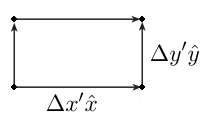
\includegraphics[scale=.8]{immagini/cap_7/fig7_1.png}
\end{center}
\end{figure}\\
Matematicamente questa circostanza si esprime come:
\begin{equation}
T(\Delta y'\hat{y})T(\Delta x'\hat{x})= T(\Delta x'\hat{x})T(\Delta y'\hat{y}),
\end{equation}
o, equivalentemente
\begin{equation}
\left[ T(\Delta x'\hat{x}), T(\Delta y'\hat{y})\right] =0.
\end{equation}
Espresso in termini dell'operatore quantità di moto, il commutatore delle due traslazioni si scrive:
\begin{eqnarray}
0 & = & \left[ T(\Delta x'\hat{x}), T(\Delta y'\hat{y})\right] =   \nonumber \\
 & = & \left[\left( 1-\frac{i p_x \Delta x'}{\hbar}-\frac{ {p_x} ^2 {\Delta x'}^2}{2\hbar ^2+\dots}\right), \left( 1-\frac{i p_y \Delta y'}{\hbar}-\frac{ {p_y} ^2 {\Delta y'}^2}{2\hbar ^2+\dots}\right) \right] = \nonumber  \\
& = & -\frac{1}{\hbar ^2}\left[p_x, p_y \right]\Delta x' \Delta y' + \dots
\end{eqnarray}
Ma per l'arbitrarietà degli spostamenti $\Delta x'$ e  $\Delta y'$ questa condizione conduce a
\begin{equation}
\left[p_x , p_y\right] =0,
\end{equation}
o, più in generale
\begin{equation}
\left[p_i , p_j\right] =0.
\end{equation}
Questo significa che \textbf{tutte e tre le componenti dell'impulso di una particella possono avere simultaneamente valori determinati}.\\
Stabiliamo le \textbf{regole di commutazione tra gli operatori impulso e gli operatori coordinate}. A tale scopo deriviamo dapprima la regola di commutazione tra l'operatore di posizione e l'operatore di traslazione infinitesima. Applicando ad un generico autoket della posizione separatamente l'operatore $\vec{x}\ T(d\vec{x}')$ o l'operatore$T(d\vec{x}')\ \vec{x}$ otteniamo:
\begin{eqnarray}
& & \vec{x}\ T(d\vec{x}')\vert \vec{x}' \rangle = \vec{x}\vert\vec{x}'+d\vec{x}'\rangle =\underbrace{\vec{x}'+d\vec{x}'}_{\textrm{autoval.}}\vert\vec{x}'+d\vec{x}'\rangle ,  \\
 \nonumber \\
& & T(d\vec{x}')\ \vec{x} \vert \vec{x}' \rangle = \underbrace{\vec{x}'}_{\textrm{autoval.}} T(d\vec{x}')\vert \vec{x}'\rangle = \vec{x}'\vert \vec{x}'+d\vec{x}'\rangle ,
\end{eqnarray}
da cui, sottraendo membro a membro
\begin{equation}
\left[\vec{x}, T(d\vec{x}')\right]\vert \vec{x}' \rangle = d\vec{x}' \vert \vec{x}' \rangle ,
\end{equation}
ma poiché uno stato arbitrario $\vert \alpha \rangle $ può essere sempre espresso come combinazione lineare di autostati della posizione, la precedente equazione vale per uno stato arbitrario e può dunque essere considerata un'identità operatoriale:
\begin{equation}
\left[\vec{x}, T(d\vec{x}')\right] = d\vec{x}'  .
\end{equation}
In termini dell'operatore impulso il commutatore si scrive
\begin{equation}
\left[ \vec{x}, 1- \frac{i}{\hbar}\vec{p}\cdot d\vec{x}'\right] =-\frac{i}{\hbar}\left(d\vec{x}'\cdot \vec{p}-\vec{p}\cdot d\vec{x}' \right) =d\vec{x}' .
\end{equation}
Consideriamo allora la componente i-esima di questa equazione e consideriamo uno spostamento $d\vec{x}'$ nella direzione dell'asse $j$. Troviamo in tal modo:
\begin{equation}
-\frac{i}{\hbar}\left( x_ip_j-p_jx_i\right) =\delta _{ij},
\end{equation}
ossia
\begin{equation}
\left[ x_i, p_j \right] =\delta _{ij}.
\end{equation}
Questa equazione dimostra che \textbf{la coordinata e la componente dell'impulso di una particella non possono essere misurate simultaneamente lungo uno stesso asse. In particolare, allora, la particella non può trovarsi in un punto determinato dello spazio e, al tempo stesso, avere una quantità di moto determinata.} D'altra parte, le precedenti relazioni di commutazione dimostrano che la coordinata della particella lungo uno degli assi può avere un valore determinato simultaneamente con le componenti dell'impulso secondo gli altri due assi.\\
La relazione di indeterminazione generale
\begin{equation}
\langle \left( \Delta A\right)^2\rangle \langle \left( \Delta B\right)^2\rangle \geq \frac{1}{4}\vert \langle \left[A,B\right] \rangle \vert ^2 ,
\end{equation}
derivata precedentemente per una coppia qualunque di operatori hermitiani $A$ e $B$, può essere applicata qui al caso gli operatori $x$ e $p_x$ per ottenere
\begin{equation}
\Delta x \cdot \Delta p_x \geq \frac{\hbar}{2} ,
\end{equation}
dove si è posto $\Delta x = \sqrt{\left(\Delta x\right) ^2}$ e $\Delta p_x = \sqrt{\left(\Delta p_x\right) ^2}$. La precedente equazione costituisce la famosa \textbf{relazione di indeterminazione di Heisenberg}, derivata da Heisenberg nel 1957.\\
L'insieme delle regole di commutazione
\begin{eqnarray}
& &\left[ x_i, x_j\right]=0 \nonumber\\
& &\left[ p_i, p_j\right]=0\\
& &\left[ x_i, p_j\right]=i\hbar \delta _{ij}\nonumber 
\end{eqnarray}
vengono dette \textbf{relazioni di commutazione canoniche} e costituiscono uno dei fondamenti della meccanica quantistica.\\
È evidente la somiglianza di queste relazioni con le relazioni
\begin{eqnarray}
& &\left\{ x_i, x_j\right\}=0 \nonumber\\
& &\left\{ p_i, p_j\right\}=0\\
& &\left\{ x_i, p_j\right\}=\delta _{ij}\nonumber 
\end{eqnarray}
valida per le \textbf{parentesi di Poisson} nella meccanica classica. Fu \textbf{Dirac} ad osservare per primo questa circostanza. Egli postulò allora che \textbf{le varie relazioni di commutazione della meccanica quantistica possono essere ottenute dalle corrispondenti relazioni classiche semplicemente sostituendo alle parentesi di Poisson i commutatori nel modo seguente:}
\begin{equation}
\left\{ \quad, \quad \right\} _{\textrm{classica}} \rightarrow \frac{i}{\hbar}\left[ \quad, \quad \right] .
\end{equation}
Questa ipotesi è consistente con il fatto che quando si passa al limite classico, l'operatore $i\left[ \quad, \quad \right]$ in prima approssimazione diventa zero.\\
È evidente tuttavia che l'assunzione di Dirac non consente comunque di stabilire, sulla base del limite classico, per quelle quantità, quali lo spin, che non hanno analogo classico.
\section[L'operatore impulso nella rappresentazione delle coordinate. Autofunzioni dell'impulso]{L'operatore impulso nella rappresentazione \\delle coordinate. Autofunzioni dell'impulso \footnote{S1.7, LL15}}
Consideriamo ora come si esprime l'operatore \textbf{impulso nella rappresentazione elle coordinate.}\\
A tale scopo esaminiamo nuovamente l'azione dell'operatore di traslazione infinitesima su un generico vettore di stato $\vert \alpha \rangle$. Riferendoci per semplicità al caso di una singola dimensione spaziale ed indicando per convenienza con $\Delta x'$ lo spostamento infinitesimo, abbiamo:
\begin{eqnarray}
\langle x' \vert T(dx') \vert \alpha \rangle 
& = & \langle x' \vert \left(1-\frac{i}{\hbar}p\ dx'\right) \vert \alpha \rangle = \langle x' \vert \left(1+\frac{i}{\hbar}p\ dx'\right) ^+ \vert \alpha \rangle = \nonumber \\
& = & \langle x'-dx'\vert \alpha \rangle = \langle x'\vert \alpha \rangle  - dx' \frac{\partial}{\partial x'} \langle x'\vert \alpha \rangle 
\end{eqnarray}
\begin{equation}
 \Rightarrow \frac{i}{\hbar}\langle x'\vert p \vert \alpha \rangle = \frac{\partial}{\partial x'}\langle x'\vert \alpha \rangle ,
\end{equation}
o anche
\begin{equation}
\label{eq:cap7_4}
\Rightarrow \langle x'\vert p \vert \alpha \rangle =-i\hbar\frac{\partial}{\partial x'}\langle x'\vert \alpha \rangle ,
\end{equation}
da cui segue anche:
\begin{equation}
\langle x'\vert p \vert x'' \rangle =-i\hbar\frac{\partial}{\partial x'}\delta (x'-x'').
\end{equation}
Dall'eq.\eqref{eq:cap7_4} possiamo derivare un'espressione esplicita per gli elementi di matrice $\langle \beta \vert p\vert \alpha \rangle $ in termini della f.d.o degli stati $\vert \beta \rangle $ ed $\vert \alpha \rangle $:
\begin{eqnarray}
\label{eq:cap7_5}
\langle \beta \vert p \vert \alpha \rangle &=& \int dx' \ \langle \beta \vert x' \rangle \left( -i\hbar \frac{\partial}{\partial x'}\right) \langle x' \vert \alpha \rangle  \nonumber \\
& = &\int dx' \ \psi _{\beta} ^* (x) \left( -i\hbar \frac{\partial}{\partial x'}\right) \psi _{\alpha}  (x') .  
\end{eqnarray}
Frequentemente si usa indicare un operatore con la sua rappresentazione nella base delle coordinate. Nel caso dell'operatore impulso questa identificazione conduce allora a
\begin{equation}
\label{eq:cap7_6}
p_x= -i\hbar \frac{\partial}{\partial x} ,
\end{equation}
o, nel caso generale di tre dimensioni
\begin{equation}
\vec{p}= -i\hbar \vec{\nabla}.
\end{equation}
Questa identificazione va intesa esattamente nel senso indicato dall'equazione \eqref{eq:cap7_5}.\\
Introduciamo ora gli \textbf{autostati dell'operatore impulso}, ossia gli stati per i quali l'impulso della particella ha un valore determinato. Continuando per semplicità a considerare il caso di una dimensione, questi stati soddisfano l'equazione
\begin{equation}
p | p' \rangle = p' | p' \rangle.
\end{equation}
Le funzioni d'onda corrispondenti agli autostati dell'impulso, ossia le ampiezze $\langle x' | p' \rangle$, sono anche dette \textbf{autofunzioni dell'operatore impulso}. L'espressione esplicita per queste autofunzioni può essere ottenuta considerando l'eq. \eqref{eq:cap7_4} nel caso in cui $| \alpha \rangle$ sia un autostato dell'impulso:
\begin{equation}
\langle x' | p | p' \rangle = -i \hbar \frac{\partial}{\partial x'} \langle x' | p' \rangle,
\end{equation}
\noindent ossia
\begin{equation}
\label{eq:cap7_7}
-i \hbar \frac{\partial}{\partial x'} \langle x' | p' \rangle = p' \langle x' | p' \rangle.
\end{equation}
Vediamo allora che, in generale, l'autostato di un operatore e la corrispondente autofunzione soddisfano la stessa equazione purché si intenda, nel secondo caso, identificare l'operatore con la sua espressione nella rappresentazione delle coordinate, come in eq. \eqref{eq:cap7_6}.\\
La soluzione dell'equazione differenziale \eqref{eq:cap7_7} per le \textbf{autofunzioni dell'operatore impulso} è
\begin{equation}
\label{eq:cap7_8}
\Psi_{p'}(x') \equiv \langle x' | p' \rangle = \mathcal{N} e^{\frac{i}{\hbar}p'x'},
\end{equation}
dove $\mathcal{N}$ è una costante di normalizzazione da determinare. Il significato fisico di questo risultato è evidente: \textbf{la probabilità che una particella che possiede un impulso determinato si trovi in una regione dello spazio compresa tra x e x+dx è una costante indipendente da x}:
\begin{equation}
\mathcal{P}(x,x+dx) = |\Psi_{p'}(x)|^2 dx = |\mathcal{N}|^2 dx.
\end{equation}
\noindent In altri termini, \textbf{in accordo con il principio di indeterminazione, una particella con impulso determinato ha un'indeterminazione totale sulla propria posizione nello spazio}.\\
L'equazione \eqref{eq:cap7_8} fornisce anche la corretta interpretazione della \emph{relazione di de Broglie}: una particella di impulso $p$ è descritta da una f.d.o. che è un'onda piana la cui lunghezza d'onda $\lambda$ è legata all'impulso $p$ dalla relazione
\begin{equation}
\lambda = \frac{2 \pi \hbar}{p} = \frac{h}{p}.
\end{equation}
Per determinare la costante di \textbf{normalizzazione delle autofunzioni dell'operatore impulso} consideriamo l'identità:
\begin{equation}
\langle x' | x'' \rangle = \int dp' \langle x' | p' \rangle \langle p' | x'' \rangle,
\end{equation}
che segue dalla relazione di completezza per gli autostati dell'impulso. Il primo membro di questa equazione è $\delta (x' - x'')$. Il secondo membro può essere calcolato utilizzando l'espressione esplicita delle autofunzioni $\langle x' | p' \rangle$ e l'espressione integrale della funzione $\delta$:
\begin{equation}
\delta (a) = \frac{1}{2 \pi} \int_{-\infty}^{+ \infty} dx ~ e^{i a x}.
\end{equation}
\noindent Si ottiene allora:
\begin{equation}
\delta (x' - x'') = |\mathcal{N}|^2 \int dp' ~ e^{\frac{i}{\hbar}p' (x' - x'')} = 2 \pi \hbar |\mathcal{N}|^2 \delta (x' - x'').
\end{equation}
Alternativamente:
\begin{eqnarray}
\langle p' | p'' \rangle &=& \int_{-\infty}^{+ \infty} dx' \langle p' | x' \rangle \langle x' | p'' \rangle = \nonumber \\
&=&  |\mathcal{N}|^2 \int_{-\infty}^{+ \infty} dx' ~ e^{-\frac{i}{\hbar}(p'-p'')x'}= \nonumber \\
&=&  |\mathcal{N}|^2 ~ 2 \pi \hbar ~ \delta (p'-p'') .
\end{eqnarray}
Scegliendo per convenzione $\mathcal{N}$ reale e positivo si ottiene allora
\begin{equation}
\Psi_{p'}(x') = \langle x' | p' \rangle = \frac{1}{\sqrt{2 \pi \hbar}} e^{\frac{i}{\hbar}p'x'}.
\end{equation}

\section[Funzioni d'onda nella rappresentazione degli impulsi]{Funzioni d'onda nella rappresentazione degli impulsi \footnote{S1.7, LL5}}
Consideriamo lo sviluppo di un generico vettore di stato $| \alpha \rangle$ in un autostato dell'operatore impulso:
\begin{equation}
| \alpha \rangle = \int dp' ~ | p' \rangle \langle p' | \alpha \rangle.
\end{equation}
I coefficienti di questo sviluppo, ossia la funzione
\begin{equation}
\Phi_\alpha (p') =  \langle p' | \alpha \rangle,
\end{equation}
determinano dunque completamente lo stato $| \alpha \rangle$.\\
La funzione $\Phi_\alpha (p')$ è detta \textbf{funzione d'onda nella rappresentazione degli impulsi}, così come la funzione
\begin{equation}
\Psi_\alpha (x') =  \langle x' | \alpha \rangle
\end{equation}
è la funzione d'onda nella rappresentazione delle coordinate.\\
Come $|\Psi_\alpha (x')|^2 dx'$ definisce la probabilità per il sistema di avere le coordinate nell'intervallo dato $dx'$, così pure $|\Phi_\alpha (p')|^2 dp'$ definisce \textbf{la probabilità che i valori dell'impulso appartengano all'intervallo dato dp'}:
\begin{equation}
\mathcal{P}(p', p'+dp') = |\langle p' | \alpha \rangle|^2 dp' = |\Phi_\alpha (p')|^2 dp'.
\end{equation}
Questa probabilità è normalizzata correttamente. Infatti, se lo stato $| \alpha \rangle$ è normalizzato, allora
\begin{eqnarray}
\langle \alpha | \alpha \rangle &=& \int_{-\infty}^{+\infty} dp' \langle \alpha | p' \rangle \langle p' | \alpha \rangle = \int_{-\infty}^{+\infty} dp' | \langle p' | \alpha \rangle |^2 = \nonumber \\
&=& \int_{-\infty}^{+\infty} dp' |\Phi_\alpha (p')|^2 = 1 .
\end{eqnarray}
\`E semplice derivare la trasformazione che lega la f.d.o. nella rappresentazione degli impulsi alla f.d.o. nella rappresentazione delle coordinate. Si ha
\begin{eqnarray}
\langle x' | \alpha \rangle &=& \int_{-\infty}^{+\infty} dp' \langle x' | p' \rangle \langle p' | \alpha \rangle =  \nonumber \\
&=& \frac{1}{\sqrt{2 \pi \hbar}} \int_{-\infty}^{+\infty} dp' ~ e^{\frac{i}{\hbar}p' \cdot x'} \langle p' | \alpha \rangle ,
\end{eqnarray}
o, equivalentemente:
\begin{equation}
\Psi_\alpha (x') = \frac{1}{\sqrt{2 \pi \hbar}} \int_{-\infty}^{+\infty} dp' ~ e^{\frac{i}{\hbar}p' \cdot x'} \Phi_\alpha (p').
\end{equation}
In modo analogo si deriva la trasformazione inversa:
\begin{equation}
\Phi_\alpha (p') = \frac{1}{\sqrt{2 \pi \hbar}} \int_{-\infty}^{+\infty} dx' ~ e^{-\frac{i}{\hbar}p' \cdot x'} \Psi_\alpha (x').
\end{equation}
Queste equazioni corrispondono matematicamente alle trasformate ed antitrasformate di Fourier.
\section[Pacchetti d'onda gaussiani]{Pacchetti d'onda gaussiani \footnote{S1.7}}
Una particella che si propaga con impulso $p$ definito è descritta, nella meccanica quantistica, da una f.d.o.:
\begin{equation}
\Psi_\alpha (x') = \langle x' | p' \rangle = \frac{1}{\sqrt{2 \pi \hbar}}~  e^{\frac{i}{\hbar}p' \cdot x'}
\end{equation}
che ha la forma di un'onda piana. La probabilità di osservare la particella in una determinata posizione è la stessa per qualunque punto dello spazio.\\
In una situazione fisica reale, tuttavia, una particella risulta sempre essere più o meno localizzata nello spazio. Questo comporta che anche il suo impulso non sia perfettamente determinato, o, equivalentemente, che lo stato della particella sia una sovrapposizione di stati con impulso definito. Le f.d.o. che descrivono tali stati vengono anche dette \textbf{pacchetti d'onda}.\\
Un esempio particolarmente importante di questo tipo è il \textbf{pacchetto d'onda gaussiano}, la cui f.d.o. nella rappresentazione delle coordinate è data da:
\begin{equation}
\Psi_\alpha (x') = \langle x' | \alpha \rangle = \frac{1}{(2 \pi \sigma^2)^{1/4}}~  e^{\frac{i}{\hbar}p_0 x' - \frac{x'^2}{4 \sigma^2}}.
\end{equation}
Per una particella che si trovi in questo stato, la distribuzione di probabilità per la coordinata $x$ è una gaussiana con valore aspettato nullo e varianza $\sigma^2$:
\begin{equation}
|\Psi_\alpha (x')|^2 = \frac{1}{\sqrt{2 \pi \sigma^2}}~   e^{- \frac{x'^2}{2 \sigma^2}}.
\end{equation}
Possiamo calcolare esplicitamente \textbf{i valori di aspettazione di x e $\mathbf x^2$}:
\begin{eqnarray}
\langle x \rangle &=& \langle \alpha | x | \alpha \rangle = \int_{-\infty}^{+\infty} dx' \langle \alpha | x | x' \rangle \langle x' | \alpha \rangle =  \nonumber \\
&=&  \int_{-\infty}^{+\infty} dx' x' \langle \alpha | x' \rangle \langle x' | \alpha \rangle = \int_{-\infty}^{+\infty} dx' x' |\Psi_\alpha (x')|^2 = 0,\\
\nonumber \\
\langle x^2 \rangle &=&  \int_{-\infty}^{+\infty} dx' x'^2 |\Psi_\alpha (x')|^2 = \frac{1}{\sqrt{2 \pi \sigma^2}} \int_{-\infty}^{+\infty} dx' x'^2 e^{- \frac{x'^2}{2 \sigma^2}} =\nonumber  \\
&=& \frac{2 \sigma^2}{\sqrt{\pi}} \int_{-\infty}^{+\infty} ds ~ s^2 ~e^{-s^2} = \frac{2 \sigma^2}{\sqrt{\pi}} ~ \Gamma(3/2) = \sigma^2,
\end{eqnarray}
ossia
\begin{equation}
\langle x \rangle = 0~~~~, ~~~~\langle x^2 \rangle = \sigma^2.
\end{equation}
Utilizzando l'espressione dell'operatore impulso nella rappresentazione delle coordinate possiamo calcolare anche \textbf{i valori di aspettazione di p e $\mathbf p^2$}. Troviamo:
\begin{eqnarray}
\langle \alpha | p | \alpha \rangle  &=&  \int_{-\infty}^{+\infty} dx' \langle \alpha | x' \rangle \left(-i \hbar \frac{\partial}{\partial x'} \right) \langle x' | \alpha \rangle = \nonumber\\
&=& \int_{-\infty}^{+\infty} dx' \Psi_\alpha(x')^* \left(-i \hbar \frac{\partial}{\partial x'} \right) \Psi_\alpha(x') = \nonumber \\
&=& \frac{1}{\sqrt{2 \pi \sigma^2}} \int_{-\infty}^{+\infty} dx' e^{-\frac{i}{\hbar}p_0 x' - \frac{x'^2}{4 \sigma^2}} \left(-i \hbar \frac{\partial}{\partial x'} \right) e^{\frac{i}{\hbar}p_0 x' - \frac{x'^2}{4 \sigma^2}} = \nonumber \\
&=& \frac{1}{\sqrt{2 \pi \sigma^2}} \int_{-\infty}^{+\infty} dx'  e^{- \frac{x'^2}{2 \sigma^2}} \left(p_0 + \frac{i \hbar}{2 \sigma^2} ~x' \right) = p_0
\end{eqnarray}
e
\begin{eqnarray}
\langle \alpha | p^2 | \alpha \rangle  &=& \int_{-\infty}^{+\infty} dx' \Psi_\alpha(x')^* \left(-i \hbar \frac{\partial}{\partial x'} \right)^2 \Psi_\alpha(x') = \nonumber \\
&=& \frac{1}{\sqrt{2 \pi \sigma^2}} \int_{-\infty}^{+\infty} dx' e^{-\frac{i}{\hbar}p_0 x' - \frac{x'^2}{4 \sigma^2}} \left(-i \hbar \frac{\partial}{\partial x'} \right)\left(p_0 + \frac{i \hbar}{2 \sigma^2} ~x' \right) e^{\frac{i}{\hbar}p_0 x' - \frac{x'^2}{4 \sigma^2}} = \nonumber \\
&=& \frac{1}{\sqrt{2 \pi \sigma^2}} \int_{-\infty}^{+\infty} dx'  e^{- \frac{x'^2}{2 \sigma^2}} \left(\frac{\hbar^2}{2 \sigma^2} + p_0^2 - \frac{\hbar^2}{4 \sigma^4}~x'^2 + \frac{i \hbar p_0}{\sigma^2}~x' \right) = \nonumber \\
&=& \frac{\hbar^2}{2 \sigma^2} + p_0^2 - \frac{\hbar^2}{4 \sigma^4} = p_0^2 + \frac{\hbar^2}{4 \sigma^4},
\end{eqnarray}
ossia:
\begin{equation}
\langle p \rangle = p_0~~~~, ~~~~\langle p^2 \rangle = p_0^2 + \frac{\hbar^2}{4 \sigma^4}.
\end{equation}
Per una particella descritta da un pacchetto d'onda gaussiano, i valori delle \textbf{dispersioni della posizione e dell'impulso} risultano:
\begin{eqnarray}
\langle (\Delta x)^2 \rangle &=& \langle x^2 \rangle - \langle x \rangle^2 = \sigma^2\\
\langle (\Delta p)^2 \rangle &=& \langle p^2 \rangle - \langle p \rangle^2 =  \frac{\hbar^2}{4 \sigma^4}.
\end{eqnarray}
Possiamo allora verificare la \textbf{relazione d'indeterminazione di Heisenberg}. In questo caso il prodotto delle indeterminazioni è dato da
\begin{equation}
\Delta x \cdot \Delta p = \frac{\hbar}{2}
\end{equation}
(dove si è posto $\Delta x \equiv \sqrt{\langle (\Delta x)^2 \rangle}$ e $\Delta p \equiv \sqrt{\langle (\Delta p)^2 \rangle}$ ) e non dipende da $\sigma$. Così \textbf{per un pacchetto d'onda gaussiano} abbiamo una relazione di uguaglianza, anziché la più generale relazione di disuguaglianza, ed \textbf{il prodotto $\mathbf{\Delta x \Delta p}$ assume il valore minimo possibile}.\\
La funzione d'onda nella rappresentazione degli impulsi per un pacchetto d'onda gaussiano è
\begin{eqnarray}
\Phi_\alpha(p') &=& \frac{1}{\sqrt{2 \pi \hbar}} \int_{-\infty}^{+\infty} dx'~ e^{-\frac{i}{\hbar} p' x'} \Psi_\alpha(x') = \\
&=& \frac{1}{\sqrt{2 \pi \hbar}} \frac{1}{(2 \pi \sigma^2)^{1/4}} \int_{-\infty}^{+\infty} dx'~ e^{-\frac{i}{\hbar} (p'-p_0) x' - \frac{x'^2}{4 \sigma^2}} = \nonumber \\
&=& \frac{1}{\sqrt{2 \pi \hbar}} \frac{1}{(2 \pi \sigma^2)^{1/4}} \int_{-\infty}^{+\infty} dx'~ e^{-\left(\frac{x'}{2 \sigma} + \frac{i}{\hbar} (p'-p_0) \sigma \right)^2 - \frac{(p'-p_0)^2}{\hbar^2}\sigma^2} = \nonumber \\
&=&  \frac{1}{\sqrt{\pi}} \left(\frac{16 \sigma^4}{4 \hbar^2 \cdot 2 \pi \sigma^2} \right)^{1/4} e^{-\frac{(p'-p_0)^2}{\hbar^2/\sigma^2}} \int_{-\infty}^{+\infty} ds ~e^{-s^2},
\end{eqnarray}
ossia
\begin{equation}
\Phi_\alpha(p') = \left(\frac{2 \sigma^2}{\pi \hbar^2} \right)^{1/4} e^{-\frac{(p'-p_0)^2}{\hbar^2/\sigma^2}}.
\end{equation}
Per un pacchetto d'onda gaussiano \textbf{la funzione d'onda nella rappresentazione degli impulsi è pure una gaussiana}. Il valore di aspettazione e la varianza di questa gaussiana sono $p_0$ e $\hbar^2/4 \sigma^2$ rispettivamente.\\
L'espressione ottenuta per la f.d.o. nella rappresentazione degli impulsi offre una via alternativa per calcolare i valori di aspettazione di $p$ e $p^2$:
\begin{eqnarray}
\langle p \rangle &=& \int_{-\infty}^{+\infty} dp' p' |\Phi_\alpha(p')|^2 = p_0\\
\langle p^2 \rangle &=& \int_{-\infty}^{+\infty} dp' p'^2 |\Phi_\alpha(p')|^2 = p_0^2 + \frac{\hbar^2}{4 \sigma^2}.
\end{eqnarray}
\section{Operatore posizione nella rappresentazione degli impulsi}
Per derivare l'espressione dell'operatore posizione nella rappresentazione degli impulsi calcoliamo esplicitamente gli elementi di matrice $\langle p' | x | p'' \rangle$. Si~ha
\begin{eqnarray}
\langle p' | x | p'' \rangle &=& \int dx' \langle p' | x | x' \rangle \langle x' | p'' \rangle = \nonumber\\
&=& \int dx' x' \langle p' | x' \rangle \langle x' | p'' \rangle = \nonumber\\
&=& \frac{1}{2 \pi \hbar} \int dx' x' e^{-\frac{i}{\hbar} (p'-p'') x'} = \nonumber \\
&=& i \hbar \frac{\partial}{\partial p'} ~\delta(p' - p'').
\end{eqnarray}
Dunque:
\begin{equation}
\langle p' | x | p'' \rangle = i \hbar~ \frac{\partial}{\partial p'} ~\delta(p' - p'').
\end{equation}
Siamo dunque in grado di esprimere, utilizzando la rappresentazione degli impulsi, l'elemento di matrice dell'operatore posizione tra due stati $| \alpha \rangle$ e $| \beta \rangle$ arbitrari:
\begin{eqnarray}
\langle \alpha | x | \beta \rangle &=& \int dp' dp'' \langle \alpha | p' \rangle \langle p' | x | p'' \rangle \langle p'' | \beta \rangle = \nonumber \\
&=& \int dp' dp'' \langle \alpha | p' \rangle \left(i \hbar \frac{\partial}{\partial p'} \right) \delta(p'-p'') \langle p'' | \beta \rangle,
\end{eqnarray}
ossia, effettuando l'integrale in $dp''$:
\begin{eqnarray}
\langle \alpha | x | \beta \rangle &=& \int dp' \langle \alpha | p' \rangle \left(i \hbar \frac{\partial}{\partial p'} \right) \langle p' | \beta \rangle = \nonumber\\
&=& \int dp'~ \Phi_\alpha(p')^* \left(i \hbar \frac{\partial}{\partial p'} \right) \Phi_\beta(p').
\end{eqnarray}
Vediamo allora che per l'operatore posizione nella rappresentazione degli impulsi vale la relazione
\begin{equation}
x = i \hbar~ \frac{\partial}{\partial p} .
\end{equation} %DEFINITIVO
\chapter{Dinamica Quantistica}
\section[Evoluzione temporale degli stati]{Evoluzione temporale degli stati.\\Operatore Hamiltoniano ed equazione di Schr\"{o}dinger\footnote{S2.1, LL8} }
Nella meccanica quantistica il vettore di stato (o equivalentemente la funzione d'onda) determina in modo completo lo stato di un sistema fisico. Ciò significa che questo vettore, dato in un certo istante, ne definisce anche il comportamento in tutti gli istanti successivi. Il problema che ci proponiamo qui di affrontare è lo studio dell'\textbf{evoluzione dinamica dei vettori di stato}.\\
Consideriamo un sistema fisico descritto, ad un certo istante di tempo $t_0$, dal vettore di stato $\vert \alpha, t_0 \rangle$. In generale lo stato del sistema evolverà nel tempo e sarà descritto, a ciascun istante di tempo successivo, $t>t_0$, dal vettore $\vert \alpha, t\rangle$.\\
Poiché il vettore di stato $\vert \alpha, t \rangle$ deve essere determinato univocamente dal vettore di stato al tempo iniziale $\vert \alpha, t \rangle$, possiamo definire una relazione tra i due vettori nella forma: \begin{equation}
\vert \alpha, t \rangle = U(t,t_0)\vert \alpha, t_0 \rangle,
\end{equation}
dove $U(t,t_0)$ è un operatore chiamato \textbf{operatore di evoluzione temporale}.\\
Per la \textbf{conservazione della probabilità}, il vettore si stato deve rimanere normalizzato ad uno a tutti gli istanti di tempo:
\begin{eqnarray}
\langle \alpha, t \vert \alpha, t \rangle & = &
\langle \alpha, t_0 \vert U^+ (t,t_0) U(t,t_0)\vert \alpha, t \rangle = \nonumber\\
& = & \langle \alpha, t_0 \vert \alpha, t_0 \rangle.
\end{eqnarray}
Questo comporta pertanto che  \textbf{l'operatore di evoluzione temporale} debba essere \textbf{unitario}:
\begin{equation}
U^+ (t,t_0) U(t,t_0)=1.
\end{equation}
Evidentemente, nel limite $t\longrightarrow t_0$ l'operatore di traslazione temporale deve ridursi all'operatore identità. Inoltre, l'evoluzione temporale da $t_0$ a $t_1$ seguita dall'evoluzione temporale da $t_1$ a $t_2$ deve essere equivalente all'evoluzione dal tempo $t_0$ al tempo $t_2$ direttamente:
\begin{equation}
U (t_2,t_1) U(t_1,t_0)=U(t_2,t_0).
\end{equation}
Queste proprietà consentono di dedurre una semplice espressione per l'\textbf{operatore di evoluzione temporale infinitesimo}:
\begin{equation}
U(t_0+dt,t_0) = 1-i\Omega dt,
\label{eq:cap8_1}
\end{equation}
dove, in virtù della condizione di unitarietà di $U$, l'operatore $\Omega$ è hermitiano:
\begin{equation}
\Omega ^+ = \Omega.
\end{equation}
Nella meccanica classica, una traslazione temporale infinitesima può essere considerata come una trasformazione canonica:
\begin{equation}
Q_i = q_i+\dot{q}_idt, \qquad P_i = p_i+\dot{p}_idt
\end{equation}
ottenibile dalla funzione generatrice:
\begin{equation}
\Phi = \sum _i q_iP_i+ Hdt.
\label{eq:cap8_2}
\end{equation}
Ricordando che $\sum _i q_iP_i$ è la funzione generatrice della trasformazione identità, dal confronto delle eq. (\ref{eq:cap8_1}) e (\ref{eq:cap8_2}) siamo indotti a formulare l'ipotesi che l'operatore hermitiano $\Omega$ concida, a meno di un fattore di proporzionalità, con l'\textbf{operatore hamiltoniano} del sistema. L'inverso della costante di proporzionalità ha le dimensioni di un'azione e risulta essere uguale alla constante di Planck, $\hbar$. Dunque:
\begin{equation}
\Omega = \frac{H}{\hbar},
\end{equation}
e con questa identificazione:
\begin{equation}
U(t_0+dt,t_0) =1-\frac{i}{\hbar}Hdt.
\end{equation}
L'espressione derivata per l'operatore di evoluzione temporale infinitesima può essere convenientemente posta nella forma di un'equazione differenziale per l'operatore di evoluzione temporale finita, o, equivalentemente, per il vettore di stato del sistema- A tale scopo osserviamo che:
\begin{eqnarray}
& &U(t+dt,t_0)-U(t,t_0)= \nonumber \\
& &= U(t+dt,t)U(t,t_0)-U(t,t_0)= \\
& &=\left(1-\frac{i}{\hbar}Hdt \right)U(t,t_0)-U(t,t_0)=-\frac{i}{\hbar}Hdt U(t,t_0).\nonumber
\end{eqnarray}
Dividendo entrambi i membri di questa equazione per $dt$ e considerando il limite $dt \longrightarrow 0$, si ottiene quindi:
\begin{equation}
i\hbar \frac{\partial}{\partial t} U (t, t_0)= H U(t,t_0).
\label{eq:cap8_3}
\end{equation}
Questa equazione definisce completamente l'operatore di evoluzione temporale in termini dell'operatore hamiltoniano del sistema (con la condizione $U(t_0,t_0)=1).$\\
Ad un'analoga equazione pet i vettori di stato di giunge applicando entrambi i membri della (\ref{eq:cap8_3}) al kety $\vert \alpha, t_0\rangle$:
\begin{equation}
i\hbar \left( \frac{\partial}{\partial t} U (t,t_0) \right) \vert \alpha, t_0\rangle= H U(t, t_0)\vert \alpha, t_0\rangle.
\end{equation}
Poiché $\vert \alpha, t_0\rangle$ non dipende dal tempo t, possiamo espreimere questa relazione in termini del vettore di stato al tempo $t$, $\vert \alpha, t\rangle= U(t,t_0)\vert \alpha, t_0\rangle$. Si ottiene così:
\begin{equation}
i\hbar \frac{\partial}{\partial t} \vert \alpha, t \rangle = H \vert \alpha, t \rangle.
\end{equation}
Questa equazione fondamenttale della meccanica quantistica è detta \textbf{equazione di Schr\"{o}dinger. Se si conosce la forma dell'operatore hamiltoniano, allora l'equazione di Schr\"{o}dinger consente di determinare i vettori di stato del sistema fisico dato.}
\section[Stati stazionari]{Stati stazionari\footnote{S2.1, LL10}}
\textbf{L'hamiltoniano di un sistema isolato, o di un sistema che si trova in un campo esterno costante e non variabile non può contenere il tempo esplicitamente.} Ciò risulta dal fatto che tutti gli istanti di tempo sono equivalenti rispetto a tale sistema fisico.\\
\textbf{Per tali sistemi, la soluzione dell'equazione di Schr\"{o}dinger assume una forma particolarmente semplice}. L'operatore di evoluzione temporale è infatti:
\begin{equation}
U(t,t_0)= e^{-i\frac{i}{\hbar}H(t-t_0)},
\end{equation}
ed i vettori di stato si scrivono nella forma:
\begin{equation}
\vert \alpha, t \rangle = e^{-i\frac{i}{\hbar}H(t-t_0)}\vert \alpha, t_0 \rangle.
\end{equation}
Queste conclusioni possono essere verificate per sostituzione diretta nell'equazione di Schr\"{o}dinger.\\
Se l'hamiltoniano di un sistema fisico non dipende esplicitamente dal tempo, risulta possibile considerare, per tale sistema, \textbf{gli stati in cui l'energia assume un valore determinato}. Questi stato sono detti \textbf{stati stazionari} e corrispondono agli autostati dell'operatore hamiltoniano, soddisfano cioè l'equazione agli autovalori:
\begin{equation}
H|n\rangle = E_n |n \rangle.
\end{equation}
Consideriamo l'equazione di Schr\"{o}dinger per uno stato stazionario:
\begin{equation}
i\hbar \frac{\partial}{\partial t}|n,t\rangle = H |n,t \rangle = E_n |n, t \rangle.
\end{equation}
Questa equazione può \textbf{essere integrata direttamente rispetto al tempo, e dà}
\begin{equation}
|n,t\rangle = e^{-\frac{i}{\hbar}E_n t}\vert n, 0\rangle,
\label{eq:cap8_4}
\end{equation}
dove si è considerato, per semplicità $t_0=0$. Allo stesso risultato si giunge ovviamente applicando l'operatore di evoluzione temporale allo stato $\vert n, 0\rangle$:
\begin{equation}
\vert n, t \rangle = U(t,0) \vert n, 0 \rangle = e^{-\frac{i}{\hbar}H t}\vert n, 0\rangle= e^{-\frac{i}{\hbar}E_n t}\vert n, 0\rangle.
\end{equation}
L'equazione (\ref{eq:cap8_4}) determina la dipendenza dal tempo dei vettori di stato corrispondenti agli stati stazionari. Essa indica, in particolare, che \textbf{se il sistema si trova in un determinato istante in un autostato dell'hamiltoniana, esso resta in tale autostato per tutti gli istanti seguenti. Equivalentemente, possiamo affermare che se, nello stato dato, l'energia ha un valore determinato, questo valore resterà costante nel tempo.} Questo risultato esprime in meccanica quantistica la \textbf{legge di conservazione dell'energia per i sistemi isolati, o sistemi che si trovano in campi esterni non dipendenti dal tempo}.\\
Calcoliamo il valore di aspettazione di un generico osservabile $A$ in uno stato stazionario, come funzione del tempo. Utilizzando l'eq.(\ref{eq:cap8_4}) troviamo:
\begin{eqnarray}
\langle A \rangle _t &=& \langle n, t \vert A \vert n, t \rangle= \langle n, 0 \vert e^{\frac{i}{\hbar}E_n t}A e^{-\frac{i}{\hbar}E_n t}\vert n, 0 \rangle \nonumber \\
& = &\langle n, 0 \vert A \vert n, 0 \rangle = \langle A \rangle _0.
\end{eqnarray}
Pertanto \textbf{il valore di aspettazione di un'osservabile in un autostato dell'energia non cambia nel tempo. Per questo motivo tali stati vengono detti stati stazionari.}\\
Un generico vettore di stato $\vert \alpha \rangle $ può essere sviluppato in autostati dell'energia. All'istante iniziale $t=0$ tale sviluppo ha la forma:
\begin{equation}
\vert \alpha , t=0\rangle = \sum _n \vert n \rangle \langle n \vert \alpha, t=0 \rangle = \sum _n c_n(0)\vert n \rangle.
\end{equation}
Questo sviluppo consente di derivare una semplice espressione per lo stato evoluto ad un tempo $t$ successivo. A tale scopo è sufficiente applicare allo stato l'operatore di \textbf{evoluzione temporale}:
\begin{eqnarray}
\vert \alpha, t \rangle &=& U (t,0)\vert \alpha, t=0 \rangle = \sum _n c_n (0) e^{-\frac{i}{\hbar}H t}  \vert n \rangle = \nonumber \\
& = &\sum _n c_n (0) e^{-\frac{i}{\hbar}E_n t}  \vert n \rangle.
\end{eqnarray}
In altre parole il generico coefficiente dello sviluppo varia nel tempo come:
\begin{equation}
c_n (t=0) \rightarrow c_n(t)=e^{-\frac{i}{\hbar}E_n t} c_n (0).
\end{equation}
I moduli quadri $\vert c_n(t)\vert^2$ dei coefficienti dello sviluppo rappresentano, come al solito, le probabilità dei diversi valori dell'energia del sistema. La precedente equazione mostra come tali probabilità restano \textbf{costanti nel tempo}.\\
Il formalismo sin qui sviluppato si estende facilmente al caso in cui gli autovalori dell'energia formino uno \textbf{spettro continuo}.
\section[ Equazione d'onda di Schrödinger]{Equazione d'onda di Schr\"{o}dinger\footnote{S2.4, LL17}}
Esaminiamo l'\textbf{evoluzione temporale dei vettori di stato nella rappresentazione delle coordinate}. In altre parole studiamo il comportamento della funzione d'onda
\begin{equation}
\psi (\vec{x'}, t) = \langle \vec{x'}\vert \alpha, t \rangle
\end{equation}
come funzione del tempo.\\
La forma specifica dell'equazione di Schr\"{o}dinger di un sistema fisico è determinata dal suo hamiltoniano, che acquista perciò un'importanza fondamentale in tutto l'apparato della meccanica quantistica.\\
In perfetta corrispondenza con l'espressione classica, in meccanica quantistica \textbf{l'hamiltoniano di una particella sottoposta ad un campo esterno è}
\begin{equation}
H= \frac{\vec{p}^{\ 2}}{2m}+V(\vec{x}),
\label{eq:cap8_5}
\end{equation}
dove $V(\vec{x})$ è l'energia potenziale della particella nel campo esterno.		
L'equazione che determina l'evoluzione temporale della f.d.o. si ottiene moltiplicando a sinistra per il bra $\langle \vec{x'}\vert $ l'equazione di Schr\"{o}dinger per i vettori di stato:
\begin{equation}
i\hbar \frac{\partial}{\partial t} \langle \vec{x'}\vert \alpha , t \rangle = \langle \vec{x'}\vert H \vert \alpha , t \rangle.
\end{equation}
Ricordando l'espressione dell'operatore impulso nella rappresentazione delle coordinate, possiamo scrivere il contributo dell'energia cinetica al secondo membro della precedente equazione nella forma
\begin{equation}
\langle \vec{x'}\vert \frac{\vec{p}^{\ 2}}{2m} \vert \alpha , t \rangle = -\frac{\hbar^2}{2m}{{\nabla}'}^2\langle \vec{x'}\vert \alpha , t \rangle
\end{equation}
dove ${{\nabla}'}^2$ è l'operatore di Laplace, o Laplaciano:
\begin{equation}
{{\nabla}'}^2= \frac{\partial ^2}{\partial {x'} ^2}+\frac{\partial ^2}{\partial {y'} ^2}+\frac{\partial ^2}{\partial {z'} ^2}.
\end{equation}
Quanto al contributo dell'energia potenziale si ha semplicemente:
\begin{equation}
\langle \vec{x'}\vert V(\vec{x}) \vert \alpha , t \rangle = V(\vec{x'})\langle \vec{x'}  \vert \alpha , t \rangle ,
\end{equation}
dove $V(\vec{x'})$ non è più un operatore.\\
raccogliendo i cari termini otteniamo l'\textbf{equazione d'onda per una particella sottoposta ad un campo esterno}:
\begin{equation}
i\hbar \frac{\partial \psi}{\partial t} = H\psi = -\frac{\hbar ^2}{2m}{\nabla '} ^2 \psi + V(\vec{x'}) \psi,
\end{equation}
con $\psi =\psi(\vec{x'}, t)$. Questa è l'equazione nella forma derivata da \textbf{Schr\"{o}dinger} nel \textbf{1926}.\\
Nella rappresentazione delle coordinate, l'equazione agli autovalori che determina gli stati stazionari si scrive
\begin{equation}
\langle \vec{x'}\vert H \vert n \rangle = E_n\langle \vec{x'} \vert n \rangle,
\end{equation}
indicando con
\begin{equation}
\psi _n (\vec{x'}) = \langle \vec{x'} \vert n \rangle
\end{equation}
le autofunzioni dell'operatore \textbf{hamiltoniano corrispondenti agli autovalori $E_n$}, ed assumendo per $H$ l'espressione (\ref{eq:cap8_5}) otteniamo:
\begin{equation}
H\psi _n = -\frac{\hbar ^ 2}{2m}{\nabla '}^2 \psi _n + V(\vec{x'})\psi _n = E_n \psi _n.
\end{equation}
Questa equazione per le autofunzioni dell'energia è detta \textbf{equazione d'onda di Schr\"{o}dinger indipendente dal tempo}.\\
\textbf{Lo spettro degli autovalori dell'energia}, determinato dall'equazione di Schr\"{o}dinger indipendente dal tempo \textbf{può essere sia discreto che continuo. Lo stato stazionario dello spettro discreto corrisponde sempre ad un moto finito della particella}, cioè ad un moto in cui la particella non si allontana all'infinito. La condizione di normalizzazione per gli autostati dello spettro discreto implica infatti:
\begin{equation}
\langle n \vert n \rangle = \int _{- \infty} ^{+\infty} d\vec{x'}\langle n \vert \vec{x'} \rangle \langle \vec{x'} \vert n \rangle = \int _{- \infty} ^{+\infty} d\vec{x'} \vert \psi _n (\vec{x'}) \vert ^2 =1.
\end{equation}
Ciò significa in ogni caso che $ vert \psi _n  \vert ^2$ decresce in modo sufficientemente rapido e si annulla all'infinito. In altri termini \textbf{le probabilità dei valori infiniti delle coordinate è nulla, cioè il sistema compie un moto finito o, come si dice ancora, si trova in uno stato legato}.\\
La condizione di normalizzazione
\begin{equation}
\langle n \vert n' \rangle = \delta (E_n - E_{n'})
\end{equation}
per gli autostati dello spettro continuo, implica che \textbf{l'integrale}
\begin{equation}
\int _{- \infty} ^{+\infty} d\vec{x'} \vert \psi _n (\vec{x'}) \vert ^2
\end{equation}
\textbf{diverge per le autofunzioni dello spettro continuo}.
il modulo quadro della f.d.o.,$\vert \psi _n \vert ^2 $, non dà in questo caso direttamente la probabilità dei diversi valori delle coordinate e deve essere considerato solamente come una grandezza proporzionale a questa probabilità. \textbf{La divergenza dell'integrale} $ \int  d\vec{x'} \vert \psi _n  \vert ^2$ \textbf{è sempre dovuta al fatto che $\vert \psi _n  \vert ^2$ non si annulla all'infinito (o comunque non si annulla con sufficiente rapidità)}. Si può affermare quindi che l'integrale $ \int  d\vec{x'} \vert \psi _n  \vert ^2$ calcolato all'esterno di una superficie chiusa arbitrariamente grande ma finita, continua ancora ad essere divergente. Ciò significa che, \textbf{nello stato considerato, la particella si trova all'infinito}.\\
Consideriamo l'equazione di Schr\"{o}dinger indipendente del tempo per una \textbf{particella libera}:
\begin{equation}
-\frac{\hbar ^2}{2m}\nabla ^2 \psi = E\psi.
\end{equation}
QUesta equazione \textbf{ha soluzioni finite in tutto lo spazio per qualunque valore positivo dell'energia}. Queste soluzioni, per gli stati aventi direzioni da moto determinate, sono le \textbf{autofunzioni dell'operatore impulso}, con $E= p^2/2m$:
\begin{equation}
\psi (\vec{x'}) \propto e ^{\frac{i}{\hbar}\vec{p}\cdot \vec{x'}},
\end{equation}
come si può stabilire per sostituzione diretta nell'equazione. Per la particella liber, l'operatore hamiltoniano e l'operatore impulso commutano tra loro
\begin{equation}
\left[ H, \vec{p}\ \right] = \left[ \frac{ {\vec{p}}^{\ 2}}{2m}, \vec{p}\ \right] =\vec{0},
\end{equation}
ed ammettono pertanto una base di autostati in comune.\\
\textbf{Le f.d.o. totali} (dipendenti dal tempo) degli stati stazionari della particella libera hanno la forma:
\begin{equation}
\psi (\vec{x'}, t) = c\ e^{-\frac{i}{\hbar} (Et - \vec{p}\cdot \vec{x'})}, \qquad E={\vec{p}}^{\ 2}/{2m}.
\label{eq:cap8_6}
\end{equation}
Ogni funzione di questo tipo, descrivente un'\textbf{onda piana}, descrive uno stato in cui la particella ha energia $E$ e quantità di moto $\vec{p}$ determinate. La frequenza di quest'onda ed il suo vettore d'onda sono
\begin{equation}
\omega = \frac{E}{\hbar}, \quad \vec{k}= \frac{\vec{p}}{\hbar},
\end{equation}
rispettivamente.\\
Lo spettro energetico di una particella libera è \textbf{quindi continuo e si estende da zero a} $+\infty$. \textbf{Ciascuno di questi autovalori} (ad eccezione del valore $E=0$, \textbf{è degenere, con ordine di degenerazione infinito}. Infatti a ciascun valore di $E$ non nullo corrisponde un'infinità di autofunzioni (\ref{eq:cap8_6}) che si distinguono per la direzione del vettore $\vec{p}$ di modulo fissato.
\section[Densità di corrente ed equazione di continuità]{Densità di corrente ed equazione di continuità\footnote{S2.4}}
L'integrale del modulo quadro della f.d.o. esteso ad un valore finito è la probabilità di trovare la particella in questo valore. Pertanto la quantità
\begin{equation}
\rho (\vec{x}, t) = \vert \psi (\vec{x},t) \vert ^2 = \vert \langle \vec{x}\vert \alpha, t \rangle \vert ^2
\end{equation}
rappresenta in meccanica quantistica una \textbf{densità di probabilità}.\\
Calcoliamo la derivata di questa grandezza rispetto al tempo:
\begin{equation}
\frac{\partial \rho}{\partial t} = \frac{\partial }{\partial t}\left( \psi^*\ \psi \right) = \frac{\partial \psi ^*}{\partial t}\psi + \psi^*\frac{\partial \psi}{\partial t}.
\end{equation}
Sostituiamo in queste espressione l'equazione di Schr\"{o}dinger e la sua complessa coniugata:
\begin{eqnarray}
 i\hbar \frac{\partial \psi}{\partial t} &=& -\frac{\hbar ^2}{2m} \nabla ^ 2 \psi + V \psi ,\nonumber \\
\\
 -i\hbar \frac{\partial \psi ^*}{\partial t} &=& -\frac{\hbar ^2}{2m} \nabla ^ 2 \psi ^* + V \psi ^* .\nonumber
\end{eqnarray}
Si ottiene allora
\begin{eqnarray}
\frac{\partial }{\partial t}\left(\psi^*\ \psi \right) & = & \left(-\frac{i\hbar}{2m}\nabla ^2 \psi ^* +\frac{i}{\hbar}V\psi ^*\right)\psi + \nonumber \\
& &+\psi ^* \left(\frac{i\hbar}{2m}\nabla ^2 \psi -\frac{i}{\hbar}V\psi ^*\right)=\\
&=& \frac{i\hbar}{2m}\left(\psi ^* \nabla ^2 \psi - \psi \nabla ^2 \psi ^* \right) = \nonumber \\
&=& \frac{i\hbar}{2m} \vec{\nabla}\cdot \left(\psi ^* \vec{\nabla} \psi - \psi \vec{\nabla} \psi ^* \right). \nonumber
\end{eqnarray}
Ponendo
\begin{equation}
\vec{j}=\frac{i\hbar}{2m} \left(\psi ^* \vec{\nabla} \psi - \psi \vec{\nabla} \psi ^* \right)= \frac{\hbar}{m}\ \textrm{Im}\left\{\psi ^* \vec{\nabla}\psi \right\},
\end{equation}
troviamo che il vettore $\vec{j}$ e la densità di probabilità $\rho$ soddisfano l'equazione
\begin{equation}
\frac{\partial \rho}{\partial t}+ \vec{\nabla}\cdot\vec{j}=0,
\end{equation}
analoga all'\textbf{equazione} classica \textbf{di continuità}.\\
Integrando l'equazione di continuità su un volume finito $V$ ed applicando il teorema di Gauss troviamo:
\begin{equation}
\frac{\partial }{\partial t} \int _V \rho\ dV = - \int _V \vec{\nabla}\cdot\vec{j}\ dV = -\int _S \vec{j}\cdot\vec{n}\ dS.
\end{equation}
Da qui si vede che il vettore $\vec{j}$ ha il significato di una \textbf{densità di corrente di probabilità} ed è indicato di solito semplicemente con il nome di \textbf{densità di corrente}.\\
L'interpretazione fisica dell'equazione di continuità può risultare più chiara se si considera che $\rho= \psi^* \psi$ può essere trattato alla stessa maniera di una \textbf{densità media di particelle}. Il vettore $\vec{j}$ acquista allora il significato di un flusso medio di particelle che attraversano una superficie unitaria nell'unità di tempo. Si può allora considerare l'equazione di continuità come espressione della \textbf{legge di conservazione del numero di particelle}.\\
Per la f.d.o- della \textbf{particella libera}, normalizzata come:
\begin{equation}
\psi  =  e^{-\frac{i}{\hbar} (Et - \vec{p}\cdot \vec{x'})}
\end{equation}
la densità di corrente risulta
\begin{equation}
\vec{j}= \frac{\hbar}{m}\ \textrm{Im}\left\{\psi ^* \vec{\nabla}\psi \right\}= \frac{\vec{p}}{m},
\end{equation}
e rappresenta la \textbf{velocità della particella}.\\
Questa scelta della normalizzazione corrisponde ad aver fissato da uno il numero di particelle per unità di volume:
\begin{equation}
\int _{V=1} \rho \ dV = \int _{V=1} \vert \psi \vert ^2 \ dV=1.
\end{equation}
Un'altra possibile scelta per la normalizzazione dell'onda piana è
\begin{equation}
\psi  = \sqrt{\frac{m}{p}}\ e^{-\frac{i}{\hbar} (Et - \vec{p}\cdot \vec{x'})},
\end{equation}
che descrive la corrente di particelle con flusso unitario, ossia una particella attraversa in media l'unità di superficie nell'unità di tempo. In questo caso la densità di corrente è infatti
\begin{equation}
\vec{j}=  \frac{\vec{p}}{p},
\end{equation}
ossia il vettore unitario nella direzione del moto. %DEFINITIVO
\chapter[Operatore di parità]{Operatore di parità\footnote{G4; S4.2}}
Risulta spesso utile considerare l'operatore di parità P, definito come l'operatore unitario che effettua una \textbf{trasformazione di inversione spaziale}: $\va*{x}\to-\va*{x}$. L'azione dell'operatore di parità può dunque essere definita convenientemente a partire dagli autostati della posizione $\ket{\va*{x}'}$, sui quali l'operatore agisce nel modo seguente:

\begin{equation}
  \label{eq:cap9_1}
P\ket{\va*{x}'} = \ket{-\va*{x}'} , \qquad PP^+ = 1.
\end{equation}
Poiché gli autostati della posizione costituiscono un insieme completo di stati di base, l'eq. (\ref{eq:cap9_1}) definisce \textbf{l'azione dell'operatore di parità su uno stato arbitrario $\ket{\alpha}$}:
\begin{align}
  \ket{\alpha} &= \int\dd\va*{x}' \ket{\va*{x}'}\braket{\va*{x}'}{\alpha},\\
  \nonumber \\
  P\ket{\alpha} &= \int\dd\va*{x}' P\ket{\va*{x}'}\braket{\va*{x}'}{\alpha} = \int\dd\va*{x}' \ket{-\va*{x}'}\braket{\va*{x}'}{\alpha} =\nonumber\\
  &= \int\dd\va*{x}' \ket{\va*{x}'}\braket{-\va*{x}'}{\alpha} .
\end{align}

Da questa equazione vediamo tra l'altro che se $\psi_{\alpha}\qty(\va*{x}') = \braket{\va*{x}'}{\alpha}$ è la F.d.O dello stato $\ket{\alpha}$, la f.d.o. dello stato trasformato per parità, $\ket{\alpha'} = P\ket{\alpha}$, è:
\begin{equation}
  \psi_{\alpha'}\qty(\va*{x}') = \braket{\va*{x}'}{\alpha'} = \mel{\va*{x}'}{P}{\alpha} = \braket{-\va*{x}'}{\alpha} = \psi_{\alpha}\qty(-\va*{x}')  ,
\end{equation}
o anche più brevemente, nella rappresentazione delle coordinate
\begin{equation}
  P\psi_{\alpha}\qty(\va*{x}') = \psi_{\alpha}\qty(-\va*{x}') .
\end{equation}
Applicando due volte consecutive l'operatore di parità si deve ottenere la trasformazione identità, giacche una doppia inversione spaziale non può produrre alcun cambiamento. Pertanto
\begin{equation}
  \label{eq:cap9_2}
  P^2 = 1 .
\end{equation}
Poiché l'operatore di parità è per definizione anche unitario, $P^{\dag}P=1$, da confronto con la precedente equazione segue che
\begin{equation}
  P= P^{+} ,
\end{equation}
ossia \textbf{l'operatore di parità è un operatore unitario}.
Indichiamo con $\ket{\alpha_{\lambda}}$ un autostato dell'operatore parità corrispondente all'autovalore $\lambda$:
\begin{equation}
  P\ket{\alpha_{\lambda}} = \lambda\ket{\alpha_{\lambda}} .
\end{equation}
Applicando $P^2$ allo stato $\ket{\alpha_{\lambda}}$ e considerando l'eq.(\ref{eq:cap9_2}) troviamo
\begin{equation}
  P^2 = \ket{\alpha_{\lambda}} = P\lambda\ket{\alpha_{\lambda}} = \lambda^2\ket{\alpha_{\lambda}} = \ket{\alpha_{\lambda}} ,
\end{equation}
ossia
\begin{equation}
  \lambda^2 = 1 .
\end{equation}
\textbf{Gli autovalori dell'operatore di parità possono dunque valere solo $\pm1$}:
\begin{equation}
  P\ket{\alpha_{\pm}} = \pm\ket{\alpha_{\pm}} .
\end{equation}
Da questo segue anche per le corrispondenti autofunzioni dell'operatore di parità che
\begin{equation}
  \psi_{\pm}\qty(\va*{x}') = \braket{\va*{x}'}{\alpha_{\pm}} = \pm\mel{\va*{x}'}{P}{\alpha_{\pm}} = \pm\psi_{\pm}\qty(-\va*{x}') ,
\end{equation}
ossia \textbf{le autofunzioni dell'operatore di parità corrispondenti agli autovalori $\pm1$ sono funzioni rispettivamente pari o dispari}.\\
\\
Dimostriamo ora che \textbf{se una particella è soggetta ad un campo di forze esterne il cui potenziale è una funzione pari delle coordinate, allora l'Hamiltoniano che descrive la particella commuta con l'operatore di parità}:
\begin{equation}
  \comm{H}{P} = 0 \qquad \text{se } V\qty(-\va*{x}')= V\qty(\va*{x}') .
\end{equation}
Per dimostrarlo utilizziamo la rappresentazione delle coordinate. Data una qualunque funzione $\psi\qty(\va*{x}')$ si ha:
\begin{align}
  PH\psi\qty(\va*{x}') = P\qty(-\frac{\hbar^2}{2m}\grad^2+V\qty(x'))\psi\qty(\va*{x}') =\nonumber\\
  =\qty(-\frac{\hbar^2}{2m}\grad^2+V\qty(-x'))\psi\qty(-\va*{x}') \overbrace{=}^{ V\qty(-\va*{x}')=V\qty(\va*{x}')} HP\psi\qty{\va*{x}'}  ,
\end{align}
avendo utilizzato per il termine cinetico (con notazione per semplicità unidimensionale)
\begin{align}
  P\dv{x}\psi(x)&=P\psi'(x)= \psi'(-x)=\dv{-x}\psi(-x)=-\dv{x}P\psi(x),\\
  \to P\dv[2]{x}\psi(x)&= P\dv{x}\psi'(x) = -\dv{x}P\psi'(x)= \dv[2]{x}P\psi(x) .
\end{align}
Sappiamo anche che se l'operatore di parità commuta con l'Hamiltoniano del sistema, allora P ed H ammettono una base di autostati in comune. Si conclude pertanto che \textbf{se il potenziale è una funzione pari delle coordinate, allora gli autostasti dell'Hamiltoniano possono sempre essere scelti come autostati anche dell'operatore di parità, e le corrispondenti autofunzioni risultano essere funzioni pari o dispari delle coordinate}.
\begin{equation}
  H\psi_n\qty(\va*{x})=E_n\psi_n\qty(\va*{x}), \qquad \psi_n\qty(-\va*{x})=\pm\psi_n\qty(\va*{x}) .
\end{equation}
\subsection*{Esempio}
Come esempio di quanto discusso consideriamo il caso di una buca di potenziale infinita unidimensionale centrata nell'origine delle coordinate.\\
\begin{minipage}{.4\textwidth}
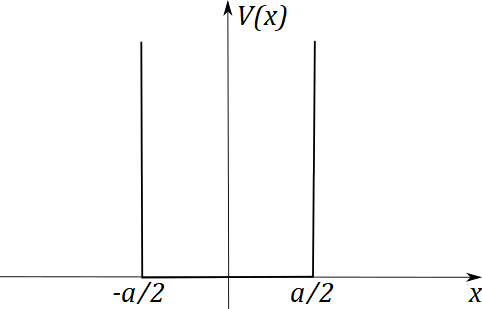
\includegraphics[width=\textwidth]{immagini/cap_9/fig_9_1.png}	
\end{minipage}
\begin{minipage}{.55\textwidth}
\begin{align}
V(x)= 
\begin{cases}
\infty \quad x<0,\\
0 \quad -a/2>x>a/2, \\
\infty \quad \textrm{fuori}.
\end{cases}
\\
\textrm{(buca di potenziale infinita)} \nonumber
\end{align}
\end{minipage}\\
In questo caso, infatti, il potenziale è una funzione pari delle coordinate e l'operatore hamiltoniano commuta con l'operatore di parità (1-dimensionale)
\begin{equation}
  \comm {H}{P}= 0
\end{equation}
Le autofunzioni di questa hamiltoniana si possono ottenere dalle autofunzioni calcolate nel caso della buca di potenziale infinita tra $x=0$ ed $x=a$ semplicemente traslando di $-a/2$ il valore della coordinata. Pertanto si trova
\begin{align}
  \psi_n(x) = \sqrt{\frac{2}{a}}\sin(\frac{n\pi}{a})\qty(x-\frac{a}{2})= \sqrt{\frac{2}{a}}\Im(e^{\frac{in\pi x}{a}}e^{-\frac{in\pi}{2}})=\nonumber\\
  =\sqrt{\frac{2}{a}}\qty[\sin(\frac{n\pi x}{a})\cos(\frac{n\pi}{2})-\cos(\frac{n\pi x}{a})\sin(\frac{n\pi}{2})] .
\end{align}
Si presentano allora due casi, a seconda che \emph{n} sia pari o dispari:
\begin{equation}
  \begin{cases}
    \psi_n(x)= (-1)^{n/2}\sqrt{\frac{2}{a}}\sin(\frac{n\pi x}{a}),\quad n=2,4,6,\;\dots\\
    \psi_n(x)= (-1)^{\frac{n+1}{2}}\sqrt{\frac{2}{a}}\cos(\frac{n\pi x}{a}),\quad n=1,3,5,\;\dots
  \end{cases}
\end{equation}
Senza perdere di generalità possiamo omettere in queste espressioni i fattori di fase irrilevanti e scrivere dunque:
\begin{equation}
  \begin{cases}
    \psi_n(x)= \sqrt{\frac{2}{a}}\sin(\frac{n\pi x}{a}),\quad n=2,4,6,\;\dots\\
    \psi_n(x)= \sqrt{\frac{2}{a}}\cos(\frac{n\pi x}{a}),\quad n=1,3,5,\;\dots
  \end{cases}
\end{equation}
Vediamo dunque che \textbf{le autofunzioni dell'hamiltoniana} sono funzioni pari o dispari delle coordinate, ossia \textbf{risultano simultaneamente autofunzioni dell'operatore di parità}.
 %DEFINITIVO
\chapter{Problemi Unidimensionali}
\section{Proprietà generali dell'equazione di Schr\"{o}dinger}
La funzione d'onda deve essere monotona e continua in tutto lo spazio.\\
le derivate della f.d.o. sono continue ovunque, anche su superfici di discontinuità del potenziale, eccetto il caso in cui $V$ diventa infinito al di fuori di tali superfici.\\
Una particella non può penetrare un generale in una regione dello spazio dove $V =\infty$, cioè dappertutto in questa regione la f.d.o. è nulla. La continuità delle f.d.o. esige che essa si annulli sul contorno di questa regione, quanto alle derivate della f.d.o. esse subiscono allora, in generale, un salto.\\
Se il potenziale $V$ è ovunque finito, anche la f.d.o. deve essere finita in tutto lo spazio (questa condizione deve essere ugualmente soddisfatta nei casi in cui $V$ diventa infinito in un punto ma non non troppo rapidamente: come $1/r^s$ con $s<2$).\\
Tutti gli autovalori dell'energia sono maggiori del minimo valore assoluto del potenziale $V$, cioè:
\begin{equation}
E_n >V_{min} \quad \forall n.
\end{equation}
Allo stesso tempo, una particella in Meccanica Quantistica può venire anche a trovarsi nelle regioni dello spazio in cui $E<V$. Anche se la probabilità $|\psi|^2$ di presenza della particella tende rapidamente a zero all'interno di tale regione, essa è però differente da zero a tutte le distanze finite.\\ \\
È semplice dimostrare che gli autovalori dell'energia sono sempre maggiori del minimo del potenziale. Si ha infatti:
\begin{equation}
E_n = \langle n | H |n \rangle = \langle n | \frac{p^2}{2m} |n \rangle + \langle n | V(x) |n \rangle.
\end{equation}
I due valori medi soddisfano poi:
\begin{equation}
\langle n | \frac{p^2}{2m} |n \rangle \geq 0,
\end{equation}
\begin{equation}
\langle n | V(x) |n \rangle = \int _{-\infty} ^{+\infty} dx' V(x')|\psi _n(x')|^2 \geq V_{min} \int _{-\infty} ^{+\infty} dx' |\psi _n(x')|^2 = V_{min},
\end{equation}
da cui segue:
\begin{equation}
E_n \geq V_{min} \qquad \textrm{c.v.d.}
\end{equation}
\section{Particella su un segmento (buca di potenziale infinita)}
Consideriamo una particella nel campo di potenziale:\\

\begin{minipage}{.5\textwidth}
\begin{align}
V(x)= 
\begin{cases}
\infty \quad x<0,\\
0 \quad 0>x>a, \\
\infty \quad x>a.
\end{cases}
\\
\textrm{(buca di potenziale infinita)} \nonumber
\end{align}	
\end{minipage}
\hspace{.5cm}
\begin{minipage}{.4\textwidth}
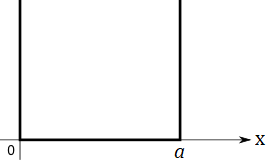
\includegraphics[width=\textwidth]{immagini/cap_10/fig_10_1.png}
\end{minipage}\\


Il moto della particella può avvenire soltanto nel segmento $\left( 0; a \right)$, giacché non è posisbile che questa penetri che questa penetri in una regione in cui $V=\infty$. Allora:
\begin{equation}
\psi(x)= 
\begin{cases}
0\quad x<0,\\
0 \quad x>a.
\end{cases}
\end{equation}
All'interno della buca, dove $V(x)=0$, l'eq. di Schr\"{o}dinger ha la forma:
\begin{equation}
-\frac{\hbar ^2}{2m}\frac{d^2 \psi}{dx^2}= E\psi\quad \Longrightarrow \quad \frac{d^2 \psi}{dx^2}=-\frac{2mE}{\hbar^2}\psi,
\end{equation}
che deve essere risolta con le condizioni al contorno:
\begin{equation}
\psi(0)=\psi(a)=0,
\end{equation}
richieste dalla continuità della f.d.o. in $x=0$ e $x=a$.\\
È facile verificare che \textbf{l'equazione non ha soluzioni corrispondenti ad $\textbf{E=0}$}, in accordo con la proprietà generale secondo cui gli autovalori dell'energia sono sempre maggiori del minimo del potenziale, in questo caso $V_{min}=0$. Infatti, per $E<0$ si può porre:
\begin{equation}
\lambda ^2 = -\frac{2mE}{\hbar ^2},
\end{equation}
e l'equazione di Schr\"{o}dinger diventa:
\begin{equation}
\frac{d^2 \psi}{dx^2}=\lambda ^2\psi.
\end{equation}
Le soluzioni di questa equazione sono della forma:
\begin{equation}
\psi(x)= Ae^{\lambda x}+ Be^{-\lambda x}.
\end{equation}
la condizione in $\psi (0)=0$ implica:
\begin{equation}
\psi(0)= A+ B=0 \quad \Rightarrow \quad B=-A,
\end{equation}
ossia
\begin{equation}
\psi(x)= 2A \sinh{\left( \lambda x \right)},
\end{equation}
e la condizione $\psi(a)=0$ non risulta mai soddisfatta.\\
Considerando allora $\textbf{E>0}$ e ponendo
\begin{equation}
k ^2 = \frac{2mE}{\hbar ^2},
\end{equation}
otteniamo per l'equazione di Schr\"{o}dinger l'espressione:
\begin{equation}
\frac{d^2 \psi}{dx^2}=-k ^2\psi.
\end{equation}
La soluzione generale di questa equazione è
\begin{equation}
\psi(x)= Ae^{ik x}+ Be^{-ik x}.
\end{equation}
la condizione $\psi (0)=0$ richiede:
\begin{equation}
\psi(0)= A+ B=0 \quad \Rightarrow \quad B=-A,
\end{equation}
ossia
\begin{equation}
\psi(x)= 2iA \sin{\left( k x \right)},
\end{equation}
la condizione in $\psi (a)=0$ implica:
\begin{equation}
k_n a= n\pi \qquad n=1,2,3\dots
\end{equation}
Questa è la condizione che determina gli \textbf{autovalori discreti dell'energia}:
\begin{equation}
E_n= \frac{\hbar ^2 {k_n}^2}{2m}=\frac{\hbar ^2 \pi n^2}{2ma^2} \quad n=1,2,3,\dots
\end{equation}
Le corrispondenti autofunzioni sono:
\begin{equation}
\psi _n = 2iA_n \sin{\left( k_n x\right)} \Rightarrow 2A_n \sin{\left( k_n x \right)},
\end{equation}
dove abbiamo tolto il fattore di fase irrilevante $i$.\\
La costante complessa $A_n$ può essere determinata dalla \textbf{condizione di normalizzazione}:
\begin{equation}
\int _{-\infty} ^{\infty} |\psi(x)| ^2 dx =1.
\end{equation}
Si trova:
\begin{eqnarray}
\int _{-\infty} ^{\infty} |\psi(x)| ^2 dx &=& \int _{0} ^{a} 4|A_n| ^2 \sin ^2 {\left( k_n x \right)}\ dx= \nonumber \\
&=& 4|A_n| ^2 \int _{0} ^{a} \left( \frac{e^{ik_n x}- e^{-ik_nx}}{2i}\right) ^2\ dx = \nonumber \\ 
&=& -|A_n| ^2 \int _{0} ^{a} \left( e^{2ik_n x}+ e^{-2ik_nx}-2\right)\  dx = \nonumber \\
&=& |A_n| ^2 \left[ 2a- 2 \int _{0} ^{a} \cos \left(\frac{2n \pi}{a} x\right)\   dx \right] = \nonumber \\
&=& |A_n| ^2 \left[ 2a- \frac{a}{n\pi} \int _{0} ^{2n\pi} \cos \alpha\   d\alpha \right] = \nonumber \\
&=& 2a|A_n|^2= 1.
\end{eqnarray}
Scegliendo la fase arbitraria della f.d.o. in modo tale che $A_n$ risulti reale e positivo otteniamo:
\begin{equation}
A_n = \frac{1}{\sqrt{2a}},
\end{equation}
ossia, in definitiva:
\begin{equation}
\psi _n (x)= \sqrt{\frac{2}{a}} \sin{\left( k_n x\right)} = \sqrt{\frac{2}{a}} \sin{\left( \frac{n \pi x}{a}\right)}; \qquad 0<x<a.
\end{equation}
È semplice verificare che \textbf{le autofunzioni sono ortogonali tra loro}:
\begin{equation}
\int _{-\infty} ^{\infty} dx\ \psi_n ^* (x) \psi _m (x) = \delta _{mn},
\end{equation}
come previsto in generale per le autofunzioni di un operatore hamiltoniano.\\ \\
\textbf{Una qualunque f.d.o.} $\mathbf{\psi (x)}$\textbf{, soluzione dell'equazione di Schr\"{o}dinger può essere espressa come combinazione lineare delle autofunzioni della hamiltoniana}:
\begin{equation}
\psi (x) = \sum _{n=1} ^{\infty} c_n \psi _n (x) = \sum _{n=1} ^{\infty} c_n \sqrt{\frac{2}{a}} \sin {\left( k_n x \right)}.
\end{equation}
L'ortonormalità delle autofunzioni può essere utilizzata per esprimere \textbf{i coefficienti} $\mathbf{c_n}$ \textbf{dello sviluppo come}:
\begin{equation}
c_n = \int _{-\infty} ^{+\infty} dx\ \psi _n ^* (x) \psi(x).
\end{equation}
Si ha infatti:
\begin{equation}
\int _{-\infty} ^{+\infty} dx\ \psi _n ^* (x) \psi(x)= \sum _m c_m \int _{-\infty} ^{+\infty} dx\ \psi _n ^* (x) \psi _m(x)= c_n.
\end{equation}
I moduli quadri $|c_n|^2$ rappresentano la probabilità che una misura dell'energia fornisca come risultato il valore $E=E_n$.\\
Il valore medio dell'energia nello stato descritto dalla f.d.o. $\psi$ è:
\begin{eqnarray}
\langle H \rangle &=& \int _{-\infty} ^{+\infty} dx\ \psi ^*(x) H \psi(x) =\sum _n c_n \int _{-\infty} ^{+\infty} dx\ \psi ^*(x) H \psi _n(x) = \nonumber \\
&=& \sum _n c_n E_n \int _{-\infty} ^{+\infty} dx\ \psi ^*(x) \psi _n(x) =\sum _n |c_n|^2 E_n .
\end{eqnarray}
Se $\psi (x)$ rappresenta la f-d-o- della particella al tempo $t=0$, la f.d.o. ad un tempo $t$ successivo è data da:
\begin{equation}
\psi (x,t) =\sum _n c_n\ e^{-\frac{i}{\hbar}E_n t}\ \psi _n (x).
\end{equation}
I risultati ottenuti consentono di derivare semplicemente gli autovalori dell'energia e le autofunzioni per una \textbf{particella in una scatola}, ossia in una buca di potenziale tridimensionale descritta dal campo:
\begin{equation}
V(x,y,z)= 
\begin{cases}
0 \quad \textrm{per}\ 0\leq x \leq a,\ 0\leq y \leq b,\ 0 \leq z \leq c;\\
\infty \quad \textrm{fuori.}
\end{cases}
\end{equation}
l'equazione di Schr\"{o}dinger per la particella all'interno della buca di potenziale si scrive:
\begin{equation}
-\frac{\hbar ^2}{2m} \left( \frac{\partial ^2 \psi}{\partial x^2}+\frac{\partial ^2 \psi}{\partial y^2}+\frac{\partial ^2 \psi}{\partial z^2}\right) = E \psi.
\end{equation}
La \textbf{hamiltoniana} si separa nella somma di tre termini, ciascuno dei quali è la  hamiltoniana di una particella libera unidimensionale:
\begin{equation}
H= H_x+H_y+H_z \qquad H_x= -\frac{\hbar ^2}{2m}  \frac{\partial ^2 \psi}{\partial x^2}, \dots
\end{equation}
Le \textbf{autofunzioni} si scompongono nel prodotto di tre autofunzioni per la buca di potenziale unidimensionale:
\begin{eqnarray}
\psi _{n_x n_y n_z} (x,y,z) &=& \psi _{n_x}(x)\psi _{n_y}(y)\psi _{n_z}(z)= \nonumber \\
&=&\sqrt{\frac{8}{abc}}\sin \frac{\pi n_x x}{a}\ \sin \frac{\pi n_y y}{b}\ \sin \frac{\pi n_z z}{c}.
\end{eqnarray}
Gli \textbf{autovalori} dell'energia sono dati dalla somma dei corrispondenti autovalori del caso unidimensionale. Scrivendo esplicitamente l'equazione agli autovalori si trova infatti:
\begin{eqnarray}
H\psi  &=& \left(H_x+H_y+H_z\right) \psi _{n_x}(x)\psi _{n_y}(y)\psi _{n_z}(z)= \nonumber \\
&=& \left( E_{n_x}+E_{n_y}+E_{n_z}\right) \psi _{n_x}(x)\psi _{n_y}(y)\psi _{n_z}(z)=  E\psi,
\end{eqnarray}
ossia, esplicitamente:
\begin{equation}
E_{n_x n_y n_z}=\frac{\hbar ^2 \pi^2}{2m} \left(\frac{{n_x}^2}{a^2}+\frac{{n_y}^2}{b^2}+\frac{{n_z}^2}{c^2}\right) \qquad n_x, n_y, n_z, = 1,2,3... 
\end{equation}
\section{Buca di potenziale: stati legati}
Consideriamo il moto di una particella nel campo di potenziale:\\

\begin{minipage}{.55\textwidth}
\begin{align}
\begin{cases}
V(x)=-V_0 \quad -a< x < a;\\
V(x)= 0 \quad x<-a,\ x> a.
\end{cases}
\\
\textrm{(buca di potenziale finita)} \nonumber
\end{align}	
\end{minipage}
\hspace{.2cm}
\begin{minipage}{.4\textwidth}
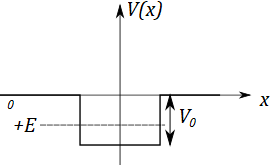
\includegraphics[width=5cm]{immagini/cap_10/fig_10_2.png}
\end{minipage}\\


Discutiamo in particolare le soluzioni dell'equazione di Schr\"{o}dinger corrispondenti agli \textbf{stati legati} della particella, ossia a valori negativi dell'energia, $\mathbf{E<0}$.\\
nelle regioni in cui il potenziale è rispettivamente nullo o pari a $-V_0$ l'equazione di Schr\"{o}dinger si scrive:
\begin{equation}
\begin{cases}
\displaystyle{-\frac{\hbar ^2}{2m}\frac{d^2 \psi}{d x^2}=-|E| \psi \qquad  x<-a,\ x> a;}\\
\\
\displaystyle{-\frac{\hbar ^2}{2m}\frac{d^2 \psi}{d x^2}= \left( V_0-|E| \right)\psi \quad  -a< x < a.}
\end{cases} 
\end{equation}
Ponendo:
\begin{equation}
\lambda ^2 = \frac{2m}{\hbar ^2}|E|, \qquad q ^2 = \frac{2m}{\hbar ^2}\left( V_0 -|E|\right),
\end{equation}
dove $q$ e $\lambda$ sono parametri reali, possiamo scrivere l'equazione di Schr\"{o}dinger nella forma:
\begin{equation}
\begin{cases}
\displaystyle{\frac{d^2 \psi}{d x^2}=\lambda ^2 \psi \qquad  x<-a,\ x> a;}\\
\\
\displaystyle{\frac{d^2 \psi}{d x^2}= -q^2 \psi \quad  -a< x < a.}
\end{cases} 
\end{equation}
Il potenziale cui è soggetta la particella è simmetrico rispetto allo scambio $x \rightarrow -x$:
\begin{equation}
V(x)= V(-x).
\end{equation}
L'operatore hamiltoniano commuta allora con l'operatore di parità:
\begin{equation}
[H;P]=0,
\end{equation}
e \textbf{le autofunzioni di $H$ possono essere scelte simultaneamente come autofunzioni dell'operatore di parità}.
Nella regione al di fuori della buca di potenziale le soluzioni all'equazione di Schr\"{o}dinger sono della forma $e^{\pm \lambda x}$. La richiesta che queste autofunzioni siano limitate all'infinito implica allora:
\begin{equation}
\begin{cases}
\psi (x) = Ae^{\lambda x} \quad x<-a;\\
\psi (x) = A'e^{\lambda x} \quad x>a.\end{cases} 
\end{equation}
All'interno della buca di potenziale le autofunzioni sono della forma $e^{\pm iq x}$, le cui combinazioni pari e dispari sono rispettivamente $\cos (qx)$ e $\sin (qx)$.\\
Consideriamo allora dapprima le \textbf{autofunzioni pari}, ossia le autofunzioni della forma:
\begin{equation}
\begin{cases}
\psi (x) = Ae^{\lambda x} \quad x<-a;\\
\psi (x) = B\cos(qx) \quad -a<x<a;\\
\psi (x) = Ae^{\lambda x} \quad x>a.\end{cases} 
\end{equation}
Per la simmetria della f.d.o. è sufficiente imporre la condizione di continuità della funzione e della sua derivata prima nel solo punto $x=-a$.\\
Automaticamente la stessa condizione risulterà soddisfatta nel punto $x=+a$. Si ha allora:
\begin{equation}
\begin{cases}
Ae^{-\lambda a} =B\cos(qa) ;\\
A \lambda e^{-\lambda a} = +Bq \sin(qa).\end{cases} 
\end{equation}
Dividendo membro a membro le due equazioni si ottiene:
\begin{equation}
q \tan (qa) =\lambda
\label{eq:cap10_1}
\end{equation}
Questa equazione determina implicitamente i possibili \textbf{autovalori dell'energia}.\\
Studiamo graficamente le soluzioni dell'equazione (\ref{eq:cap10_1}). Poniamo per convenienza:
\begin{equation}
y=qa,
\end{equation}
e
\begin{equation}
k=\frac{2mV_0 a^2}{\hbar ^2}.
\end{equation}
Poiché
\begin{equation}
\lambda ^2 a^2 = \frac{2m }{\hbar ^2}|E|a^2=k-q^2 a^2 =k-y^2,
\end{equation}
l'equazione (\ref{eq:cap10_1}) si scrive come:
\begin{equation}
\tan (y) = \frac{\sqrt{k-y^2}}{y} \qquad \qquad (y^2 \leq k).
\end{equation}
Le soluzioni dell'eq. (\ref{eq:cap10_1}) sono dunque le intersezioni della curve $\tan (y)$ e $\sqrt{k-y^2}/y$. Come appare dalla figura seguente, \textbf{i livelli di energia sono discreti}:\\
\begin{figure}[!htbp]
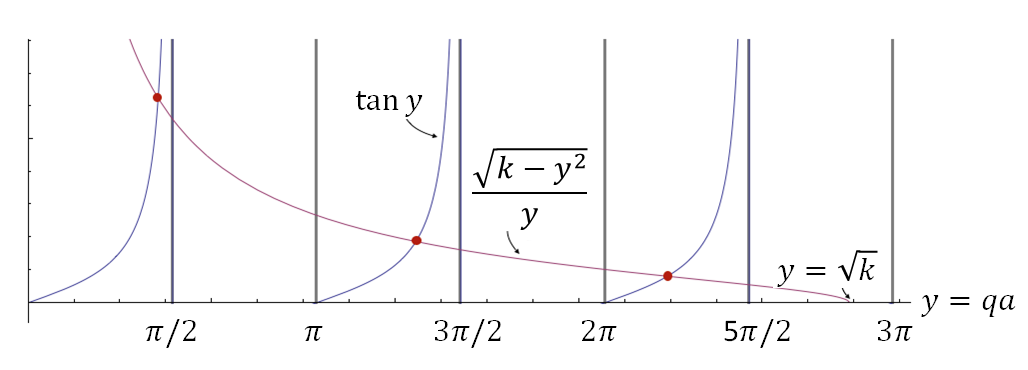
\includegraphics[width=\textwidth]{immagini/cap_10/fig_10_3.png}
\end{figure}
\\
Si noti come il numero di intersezioni cresce al crescere di $k$, ossia \textbf{esistono tanti più stati legati quanto più la buca di potenziale è profonda}.\\
inoltre esiste sempre almeno una intersezione (ed in particolare una sola per $k<\pi$), ossia \textbf{esiste sempre almeno uno stato legato per la particella}.\\
Consideriamo ora le \textbf{autofunzioni dispari}, della forma:
\begin{equation}
\begin{cases}
\psi (x) = A'e^{\lambda x} \quad x<-a;\\
\psi (x) = B'\sin(qx) \quad -a<x<a;\\
\psi (x) = -A'e^{\lambda x} \quad x>a.\end{cases} 
\end{equation}
In questo caso le condizioni di continuità della f.d.o. e della sua derivata nel punto $x=-a$ si scrivono:
\begin{equation}
\begin{cases}
A'e^{-\lambda a} =-B'\sin(qa) ;\\
A' \lambda e^{-\lambda a} = B'q \cos (qa);\end{cases} 
\end{equation}
e forniscono la condizione:
\begin{equation}
q \cot (qa) =- \lambda.
\label{eq:cap10_2}
\end{equation}
Espressa in termini di $y$ e $k$ questa equazione si scrive:
\begin{equation}
\frac{\sqrt{k-y^2}}{y}= -\cot (y) \qquad \qquad (y^2 \leq k),
\end{equation}
e le soluzioni si ottengono graficamente dalle intersezioni qui rappresentate:
\newpage
\begin{figure}[!htbp]
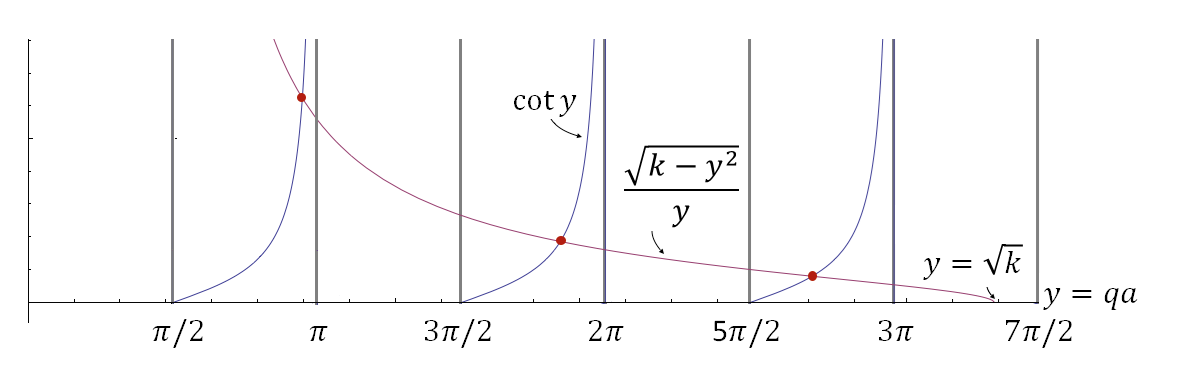
\includegraphics[width=\textwidth]{immagini/cap_10/fig_10_4.png}
\end{figure}
\[ \textrm{N.B. } \tan (y+\pi/2) = -\cot (y) \]\\
Si noti come, anche in questo caso, il numero di intersezioni cresce al crescere di $k$, ossia \textbf{il numero di stati legati cresce al crescere della profondità della buca}.\\
Tuttavia l'eq. (\ref{eq:cap10_2}) \textbf{ammette soluzioni solo se} $\mathbf{k\geq \pi^2/4}$,\textbf{ ossia}:
\begin{equation}
\frac{2mV_0 a^2}{\hbar ^2} \geq \frac{\pi ^2}{4}.
\end{equation}
Se questa condizione non è soddisfatta, esiste solo uno stato legato corrispondente ad un'autofunzione pari.
\section{Gradino di potenziale}
Consideriamo un \textbf{campo di forze in cui il potenziale presenta una discontinuità}, della forma:\\
\begin{minipage}{.55\textwidth}
\begin{equation}
V(x)=
\begin{cases}
0 \quad \textrm{ per } x<0;\\
V_0 \quad \textrm{per } x<0.
\end{cases}
\end{equation}
\end{minipage}
\hspace{.2cm}
\begin{minipage}{.4\textwidth}
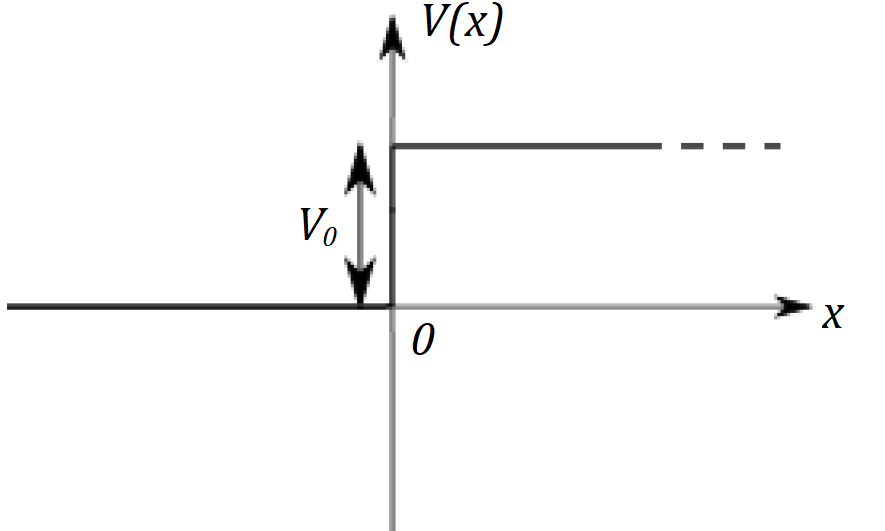
\includegraphics[width=5cm]{immagini/cap_10/fig_10_5.png}
\end{minipage}\\
Secondo la \textbf{meccanica classica}, una particella con energia $E>V_0$, che si muove in un tale campo da sinistra verso destra, arrivata alla barriera di potenziale continua a muoversi nella stessa direzione ma con velocità minore. Se invece la sua energia è $E<V_0$, arrivata alla barriera la particella si riflette da essa e riprende il moto in direzione opposta.\\
Nella \textbf{meccanica quantistica} compare un fenomeno nuovo: anche per $E>V_0$ la particella può essere riflessa dalla barriera di potenziale. Ricaviamo tale risultato.\\
L'equazione di Schr\"{o}dinger in presenza del potenziale è:
\begin{equation}
-\frac{\hbar ^2}{2m}\frac{d^2 \psi}{dx^2}+ V(x)\psi= E\psi, 
\end{equation}
ossia:
\begin{equation}
-\frac{\hbar ^2}{2m}\frac{d^2 \psi}{dx^2}= -\frac{2m}{\hbar ^2}\left( E-V(x)\right) \psi. 
\end{equation}
Considerando il caso $\mathbf{E>V_0}$ e ponendo:
\begin{equation}
k^2=\frac{2mE}{\hbar ^2} \qquad q^2=\frac{2m\left( E- V_0\right)}{\hbar ^2},
\end{equation}
otteniamo per l'equazione di Schr\"{o}dinger nelle due regioni $x<0$ ed $x>0$ la forma:
\begin{equation}
\begin{cases}
\displaystyle{\frac{d^2 \psi}{dx^2}= -k^2 \psi \quad x<0,}\\
\\
\displaystyle{\frac{d^2 \psi}{dx^2}= -q^2 \psi \quad x>0.}\\
\end{cases}
\end{equation}
Se assumiamo che la particella incidente giunga da sinistra verso destra possiamo scrivere la soluzione dell'equazione di Schr\"{o}dinger nella forma:
\begin{eqnarray}
&\psi(x)& = Ae^{ikx}+Be^{-ikx} \quad x<0,\nonumber\\
\\
&\psi(x)& = Ce^{iqx} \qquad \ \quad \qquad x>0.\nonumber
\end{eqnarray}
Ovviamente nella regione $x>0$ non esiste un'onda di ritorno. Le componenti $\displaystyle{Be^{-ikx}}$ e $\displaystyle{Ce^{iqx}}$ rappresentano invece l'\textbf{onda riflessa} e l'\textbf{onda trasmessa} dal gradino di potenziale.\\
La f.d.o. deve essere continua in tutto lo spazio, ed in particolare dunque nel punto $x=0$. Inoltre, malgrado la discontinuità del potenziale nel punto $x=0$, possiamo dimostrare che anche la derivata prima della f.d.o. deve essere continua in questo punto. Si ha infatti:
\begin{eqnarray}
& &\lim _{\varepsilon \rightarrow 0 } \left[ \left( \frac{\partial \psi}{\partial x}\right) _{\varepsilon}-\left( \frac{\partial \psi}{\partial x}\right)_{-\varepsilon}\right]=\lim _{\varepsilon \rightarrow 0 } \int_{-\varepsilon} ^{\varepsilon} dx\ \frac{d}{dx} \left( \frac{d\psi}{dx}\right)= \nonumber \\
& & = \lim _{\varepsilon \rightarrow 0 } -\frac{2m}{\hbar ^2}\int_{-\varepsilon} ^{\varepsilon} dx\ \frac{d}{dx} \left(E-V(x) \right)\psi=0,
\end{eqnarray}
dove l'ultima uguaglianza segue dal fatto che l'integrale di una funzione finita tende a zero nel limite in cui la larghezza dell'intervallo di integrazione tende a zero.\\
Imponendo la continuità della f.d.o. e della sua derivata prima nel punto $x=0$ si ottiene:
\begin{equation}
\begin{cases}
A+B=C \quad \qquad \quad \textrm{ continuità di }\psi\textrm{ in }x=0,\\
k\left(A-B \right) =qC\qquad \textrm{ continuità di }\psi '\textrm{ in }x=0.
\end{cases}
\end{equation}
Da queste due condizioni risultano determinate due costanti, $B$ e $C$, mentre la terza, $A$, dipende dalla normalizzazione della f.d.o. ossia dal flusso incidente.\\
Moltiplicando la prima equazione per q e sottraendo da questa la seconda si ottiene:
\begin{equation}
\left( q-k \right) A + \left( q+k \right)B=0,
\end{equation}
da cui:
\begin{equation}
B= \frac{k-q}{k+q}A.
\label{eq:cap10_3}
\end{equation}
Similmente, moltiplicando la prima equazione per k e sommando a questa la seconda equazione si ottiene:
\begin{equation}
2kA=\left( k+q \right)C,
\end{equation}
ossia:
\begin{equation}
C=\frac{2k}{k+q}A.
\label{eq:cap10_4}
\end{equation}
Le equazioni (\ref{eq:cap10_3}) e (\ref{eq:cap10_4}) risolvono completamente il problema posto.\\
Definiamo il \textbf{coefficiente di riflessione $R$} come il rapporto tra le densità di corrente dell'onda riflessa ($\displaystyle{Be^{-ikx}}$) e la densità di corrente dell'onda incidente ($\displaystyle{Ae^{ikx}}$):
\begin{equation}
R=\frac{|j_r|}{j_i}.
\end{equation}
Analogamente si definisce il \textbf{coefficiente di trasmissione $T$} come il rapporto tra la densità di corrente trasmessa ($\displaystyle{Ce^{iqx}}$) e la densità di corrente dell'onda incidente ($\displaystyle{Ae^{ikx}}$):
\begin{equation}
T=\frac{j_t}{j_i}.
\end{equation}
\textbf{I coefficienti di riflessione e di trasmissione rappresentano allora le probabilità che la particella incidente sul gradino di potenziale venga rispettivamente riflessa oppure trasmessa}.\\
Per una generica onda piana della forma:
\begin{equation}
\psi= Ae^{ikx},
\end{equation}
la densità di corrente è data da:
\begin{equation}
j=\frac{\hbar}{m}\Im \left(\psi ^* \frac{d\psi}{dx} \right)= |A|^2\frac{\hbar k}{m}.
\end{equation}
I coefficienti di riflessione e trasmissione risultano allora:
\begin{eqnarray}
R=\frac{|j_r|}{j_i}= \frac{|B|^2}{|A|^2}=\left(\frac{k-q}{k+q}\right)^2;\nonumber \\
\\
T=\frac{j_t}{j_i}= \frac{|C|^2 q}{|A|^2 k}=\left(\frac{4kq}{k+q}\right)^2.\nonumber 
\end{eqnarray}
Un valore di $R$ differente da zero indica una corrispondente probabilità non nulla che la particella venga riflessa dal gradino di potenziale in completo contrasto con le previsioni classiche. Tuttavia, in accordo con l'intuizione, nel limite in cui l'energia della particella è molto maggiore dell'altezza del gradino, $E\gg V_0$ ossia $k\simeq q$ la probabilità di riflessione tende a zero:
\begin{equation}
R\simeq 0\quad  \textrm{ per } E\gg V_0.
\end{equation}
Osserviamo che ovviamente è verificata la relazione:
\begin{equation}
R+T=1,
\label{eq:cap10_5}
\end{equation}
in accordo con l'interpretazione probabilistica dei coefficienti di riflessione e trasmissione.\\
L'eq. (\ref{eq:cap10_5}) può essere usata come conseguenza generale dell'equazione di continuità:
\begin{equation}
\frac{\partial \left(\psi^* \psi \right)}{\partial t}+ \frac{\partial j}{\partial x}=0,
\end{equation}
che esprime appunto la conservazione della probabilità. Poiché infatti non vi è alcuna dipendenza dal tempo nel problema, questa equazione implica che $j(x)$ è indipendente da $x$. Quindi il flusso in $x<0$ deve essere uguale al flusso in $x>0$. Si ha:
\begin{eqnarray}
j\left( x<0 \right) &=& \frac{\hbar}{m} \Im \left. \left( \psi ^* \frac{\partial \psi}{\partial x} \right) \right| _{x<0} = \nonumber \\
&=& \frac{\hbar}{m} \Im \left[ \left( A^* e^{-ikx} + B^* e^{ikx}\right)ik \left( A e^{ikx} + B e^{-ikx}\right)\right]= \nonumber \\
&=&\frac{\hbar k}{m} \Im \left[ i\left( |A|^2 - |B|^2 +AB^* e^{2ikx}- A^* B e^{-2ikx}\right)\right]= \nonumber \\
&=&\frac{\hbar k}{m} \Im \left[ i\left( |A|^2 - |B|^2 +2i \Im \left( A B^* e^{2ikx}\right) \right)\right]= \nonumber \\
&=& \frac{\hbar k}{m}\left( |A|^2 - |B|^2\right)= j_i- |j_r|,
\end{eqnarray}
e
\begin{equation}
j\left( x>0 \right) = |C| \frac{\hbar q}{m}= j_t,
\end{equation}
pertanto vale la condizione
\begin{equation}
j_i = |j_r|+ j_t,
\end{equation}
che equivale all'eq. (\ref{eq:cap10_5}) per i coefficienti di riflessione e trasmissione.\\
Un \textbf{fenomeno puramente quantistico} si osserva quando il potenziale $V_0$ è negativo ed in modulo molto grande:\\
\begin{minipage}{.7\textwidth}
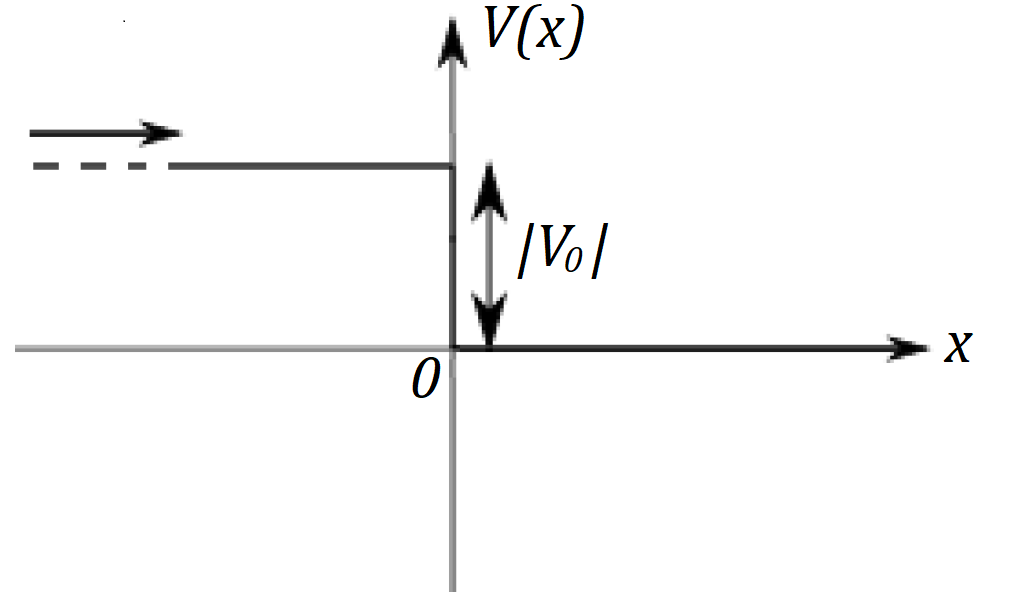
\includegraphics[width=.9\textwidth]{immagini/cap_10/fig_10_6.png}
\end{minipage}
\hspace{.5cm}
\begin{minipage}{.1\textwidth}
\[V_0<0\]
\[|V_0| \gg E\]
\end{minipage}\\ \\
Classicamente la particella proveniente da sinistra verso destra, giunta al salto di potenziale, prosegue nella sua direzione con maggiore velocità.\\
La previsione della meccanica quantistica è invece la seguente: poiché
\begin{equation}
q^2=\frac{2m}{\hbar ^2}\left( E+ |V_0| \right) \gg \frac{2mE}{\hbar ^2} = k^2,
\end{equation}
Si trova:
\begin{equation}
R=\left( \frac{q-k}{q+k} \right) ^2 \simeq 1, \qquad T=\frac{4qk}{\left( q+k \right) ^2} \simeq 0,
\end{equation}
ossia la \textbf{particella viene riflessa} con probabilità quasi uno.\\
Un altro caso che interessa considerare è quello in cui la particella incide sul gradino di potenziale con energia minore dell'altezza del gradino:\\
\begin{minipage}{.7\textwidth}
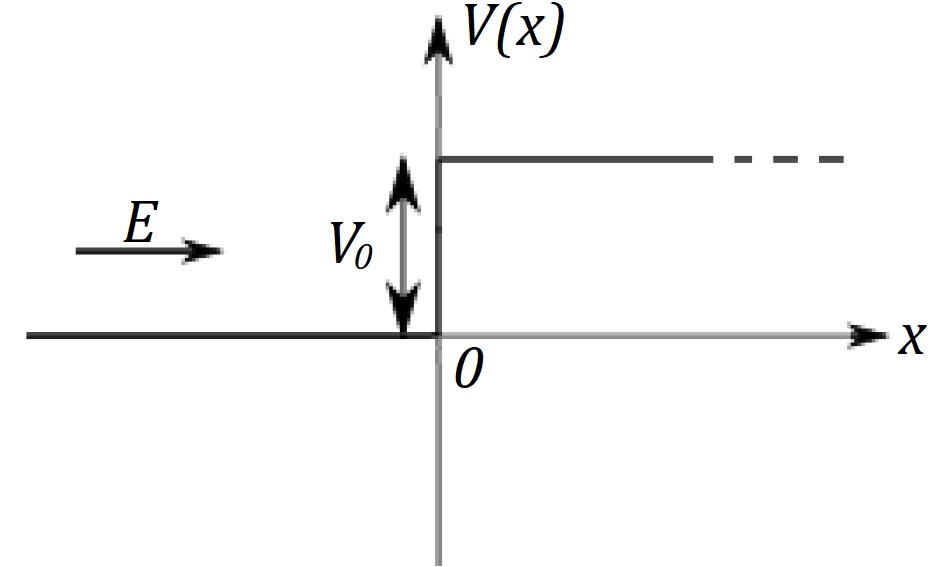
\includegraphics[width=.9\textwidth]{immagini/cap_10/fig_10_7.png}
\end{minipage}
\hspace{.5cm}
\begin{minipage}{.1\textwidth}
\[E<V_0\]
\end{minipage}\\ \\

In questo caso:
\begin{equation}
q^2=\frac{2m}{\hbar ^2}\left( E- V_0 \right)<0,
\end{equation}
ossia $q$ è immaginario. La soluzione dell'equazione di Schr\"{o}dinger, nella regione $x<0$, è della forma:
\begin{equation}
\psi (x) = Ce^{-|q|x} \qquad \qquad x<0
\end{equation}
(giacché la soluzione $\displaystyle{Ce^{+|q|x}}$ diverge all'infinito).\\
Tutti i risultati ottenuti precedentemente si modificano allora per la sostituzione:
\begin{equation}
q \rightarrow i|q|
\end{equation}
e quindi, in particolare, per i coefficienti $B$ e $C$ si ha:
\begin{equation}
B=\frac{k-i|q|}{k+i|q|}A, \qquad C=\frac{2k}{k+i|q|}.
\end{equation}
il coefficiente di riflessione $R$ risulta allora:
\begin{equation}
R=\frac{|B|^2}{|A|^2}=\frac{k-i|q|}{k+i|q|}\frac{k+i|q|}{k+i|q|}=1,
\end{equation}
mentre il coefficiente di trasmissione è nullo,
\begin{equation}
T=0,
\end{equation}
essendo sempre nulla la densità di corrente associata ad una f.d.o. reale.\\
Pertanto, come in meccanica classica, si ha in questo caso \textbf{riflessione totale}. Ciò nonostante osserviamo che la \textbf{f.d.o. non si annulla nella regione classicamente proibita} e vi è dunque una probabilità non nulla di osservare la particella in questa regione. Come vedremo in seguito, questo fenomeno puramente quantistico di penetrazione in una regione classicamente proibita consente il cosiddetto \textbf{effetto tunnel}, ossia l'attraversamento di una barriera di potenziale che bloccherebbe completamente la particella secondo la descrizione classica.
\section{Barriera di potenziale -  effetto tunnel}
Consideriamo un campo di forze il cui potenziale ha l'andamento\\
\begin{minipage}{.55\textwidth}
\begin{equation}
V(x)=
\begin{cases}
0 \qquad x<-a,\\
V_0 \quad -a<x<a,\\
0 \qquad x>-a.
\end{cases}
\end{equation}
\end{minipage}
\hspace{.2cm}
\begin{minipage}{.4\textwidth}
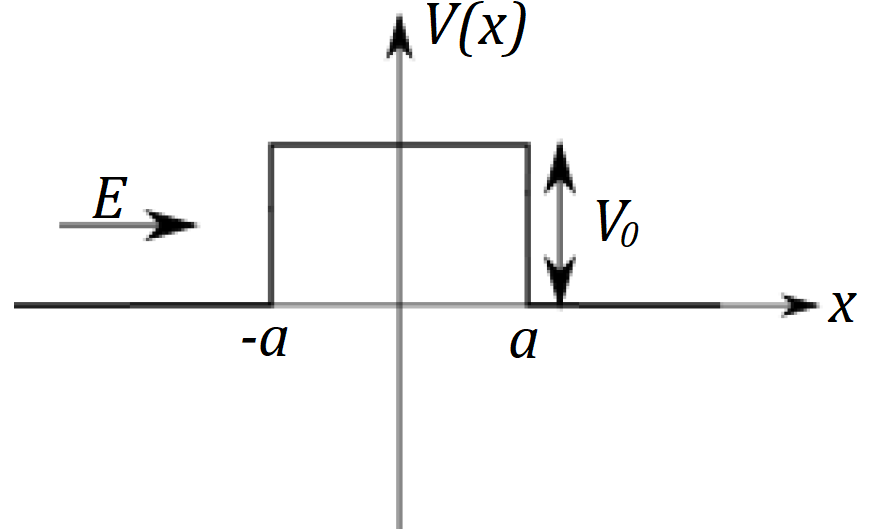
\includegraphics[width=5cm]{immagini/cap_10/fig_10_8.png}
\end{minipage}\\

Studiamo il moto della particella che giunge da sinistra con energia $\mathbf{E<V_0}$. Classicamente la particella, giunta alla barriera, viene riflessa e torna indietro.\\
Consideriamo invece la descrizione quantistica. \textbf{L'equazione di Schr\"{o}dinger} è
\begin{equation}
\begin{cases}
\displaystyle{-\frac{\hbar ^2}{2m}\frac{d^2 \psi}{d x^2}=E \psi \qquad \qquad x <-a \ \textrm{ e }\  x>a,}\\
\\
\displaystyle{-\frac{\hbar ^2}{2m}\frac{d^2 \psi}{d x^2}+V_0 \psi=E \psi \qquad -a  \leq x \leq a.}
\end{cases}
\end{equation}
Ponendo:
\begin{equation}
k^2= \frac{2mE}{\hbar ^2} \qquad \qquad \lambda ^2= \frac{2m}{\hbar ^2} \left( V_0 - E \right),
\end{equation}
dove $k$ e $\lambda $ sono parametri reali, possiamo scrivere l'equazione di Schr\"{o}dinger nella forma:
\begin{equation}
\begin{cases}
\displaystyle{\frac{d^2 \psi}{d x^2}= -k ^2 \psi \qquad  x <-a \ \textrm{ e }\  x>a,}\\
\\
\displaystyle{\frac{d^2 \psi}{d x^2}= \lambda ^2 \psi \qquad 	\ -a  < x < a.}
\end{cases}
\end{equation}
Le \textbf{soluzioni} di queste equazioni differenziali con la condizione al contorno che in assenza di barriera lo stato è rappresentato da un'onda piana che si propaga nella direzione delle $x$ positive sono:
\begin{equation}
\begin{cases}
\displaystyle{\psi (x) = e^{ikx}+Ae^{-ikx} \qquad \ x <-a,}\\
\\
\displaystyle{\psi (x) = Be^{\lambda x}+Ce^{-\lambda x} \qquad  -a< x <a,}\\
\\
\displaystyle{\psi (x) = De^{ikx} \qquad \qquad \qquad \ x >a.}
\end{cases}
\end{equation}
La \textbf{normalizzazione} scelta corrisponde ad aver fissato a
\begin{equation}
j_i= \frac{\hbar k}{m}
\end{equation}
il flusso dell'onda incidente.\\
imponendo la \textbf{continuità della f.d.o. e della sua derivata prima} nei punti $x=\pm a$ si ottiene il seguente sistema di equazioni:
\begin{equation}
\begin{cases}
\displaystyle{e^{-ika}+ Ae^{ika}= Be^{-\lambda a} + C e^{\lambda a}}\\
\\
\displaystyle{ik \left(e^{-ika}+ Ae^{ika}\right)= \lambda \left(Be^{-\lambda a} - C e^{\lambda a}\right)}\\
\\
\displaystyle{Be^{\lambda a} + Ce^{-\lambda a}= De^{ika}}\\
\\
\displaystyle{\lambda \left(Be^{\lambda a} -Ce^{-\lambda a} \right)= ikDe^{ika}}
\end{cases}
\end{equation}
Moltiplichiamo la prima equazione per $ik$ e sommiamo e sottraiamo la seconda equazione.\\
Eseguiamo le stesse operazioni sulla terza e sulla quarta equazione. Si ottiene in tal modo:
\begin{equation}
\begin{cases}
\displaystyle{2ike^{-ika}= B \left(ik+\lambda\right)e^{-\lambda a} +C \left(ik-\lambda\right)e^{\lambda a} }\\
\\
\displaystyle{2ikAe^{ika}= B \left(ik-\lambda\right)e^{-\lambda a} +C \left(ik+\lambda\right)e^{\lambda a} }\\
\\
\displaystyle{B\left(ik+\lambda\right)e^{\lambda a} + C\left(ik-\lambda\right)e^{-\lambda a} = 2ikD e^{ika}}\\
\\
\displaystyle{B\left(ik-\lambda\right)e^{\lambda a} + C\left(ik+\lambda\right)e^{-\lambda a} =0}
\end{cases}
\label{eq:cap10_10}
\end{equation}
La prima e la quarta di queste equazioni costituiscono un sistema di due equazioni nelle due incognite $B$ e $C$. Moltiplicando la prima equazione per $(ik+\lambda) e^{-\lambda a }$ e la quarta per $(ik-\lambda) e^{\lambda a }$ e sottraendo poi la quarta dalla prima si ottiene
\begin{equation}
B\left[ (ik+\lambda)^2 e^{-2\lambda a }-(ik-\lambda)^2 e^{2\lambda a }\right]= 2ik(ik+\lambda) e^{-\left(ik+\lambda\right) a },
\end{equation} 
da cui
\begin{equation}
B\left[ (-k^2+\lambda ^2+2ik\lambda) e^{-2\lambda a }-(-k^2+\lambda-2ik\lambda) e^{2\lambda a }\right]= 2ik(ik+\lambda) e^{-\left(ik+\lambda\right) a },
\end{equation}
e infine
\begin{equation}
B=\frac{ik\left(ik+\lambda \right)e^{-\left(ik+\lambda\right) a }}{\left(k^2-\lambda^2\right)\sinh \left(2\lambda a\right)+2ik\lambda \cosh\left(2\lambda a\right)}.
\end{equation}
Il coefficiente $C$ si ottiene da $B$ scambiando $\lambda \rightarrow -\lambda$:
\begin{equation}
C=\frac{-ik\left(ik-\lambda \right)e^{-\left(ik-\lambda\right) a }}{\left(k^2-\lambda^2\right)\sinh \left(2\lambda a\right)+2ik\lambda \cosh\left(2\lambda a\right)}.
\end{equation}
I coefficienti $A$ e $D$ si ottengono infine sostituendo questi risultati nella seconda e terza equazione del sistema. Si trova
\begin{eqnarray}
& 2ikAe^{ika}= B \left(ik-\lambda\right)e^{-\lambda a} +C \left(ik+\lambda\right)e^{\lambda a}=&\nonumber \\
\nonumber\\
& = \displaystyle{\frac{ik\left(-k^2-\lambda ^2 \right)e^{-2\lambda a }e^{-ika }-ik\left(-k^2-\lambda ^2 \right)e^{2\lambda a }e^{-ika }}{\left(k^2-\lambda^2\right)\sinh \left(2\lambda a\right)+2ik\lambda \cosh\left(2\lambda a\right)}=} &\nonumber \\
\nonumber \\
&\displaystyle{ =\frac{2ik\left(k^2+\lambda ^2 \right)\sinh\left(2\lambda a\right)e^{-ika}}{\left(k^2-\lambda^2\right)\sinh \left(2\lambda a\right)+2ik\lambda \cosh\left(2\lambda a\right)}},&
\end{eqnarray}
e
\begin{eqnarray}
&2ikD e^{ika} = B\left(ik+\lambda\right)e^{\lambda a} + C\left(ik-\lambda\right)e^{-\lambda a} = &\nonumber \\
\nonumber\\
& = \displaystyle{\frac{ik\left(-k^2 + \lambda ^2 +2ik\lambda\right)e^{-ika}-ik\left(-k^2 + \lambda ^2 -2ik\lambda\right)e^{-ika}}{\left(k^2-\lambda^2\right)\sinh \left(2\lambda a\right)+2ik\lambda \cosh\left(2\lambda a\right)}=} &\nonumber \\
\nonumber \\
&\displaystyle{ =\frac{-4k^2\lambda e^{-ika}}{\left(k^2-\lambda^2\right)\sinh \left(2\lambda a\right)+2ik\lambda \cosh\left(2\lambda a\right)}},&
\end{eqnarray}
ossia:
\begin{equation}
A=\frac{\left(k^2+\lambda ^2\right)\sinh\left(2\lambda a \right)e^{-2ika}}{\left(k^2-\lambda^2\right)\sinh \left(2\lambda a\right)+2ik\lambda \cosh\left(2\lambda a\right)},
\end{equation}
e
\begin{equation}
D=\frac{2ik\lambda e^{-2ika}}{\left(k^2-\lambda^2\right)\sinh \left(2\lambda a\right)+2ik\lambda \cosh\left(2\lambda a\right)}.
\end{equation}
La quantità che ci interessa calcolare è il \textbf{coefficiente di trasmissione}
\begin{equation}
T=\frac{j_t}{j_i}=|D|^2,
\end{equation}
che risulta dunque valere
\begin{equation}
T=\frac{4k^2 \lambda ^2}{\left(k^2-\lambda^2\right) ^2\sinh ^2\left(2\lambda a\right)+4k^2\lambda ^2\cosh ^2\left(2\lambda a\right)},
\end{equation}
ossia
\begin{equation}
T=\frac{4k^2 \lambda ^2}{\left(k^2+\lambda^2\right) ^2\sinh ^2\left(2\lambda a\right)+4k^2\lambda ^2}.
\end{equation}
Il risultato per questo coefficiente (diverso da zero) implica che \textbf{vi è una probabilità non nulla che la particella attraversi la barriera di potenziale}. Questo fenomeno, puramente quantistico, è noto con il nome di \textbf{effetto tunnel}.\\
Frequentemente risulta soddisfatta la condizione
\begin{equation}
2\lambda a \gg 1.
\end{equation}
Poiché
\begin{equation}
\frac{1}{\lambda}=\frac{\hbar}{\sqrt{2m\left(V_0 - E \right)}}=\frac{\hbar}{\sqrt{2mE\left(V_0/E - 1 \right)}}=\frac{\hbar /p}{\sqrt{\left(V_0/E - 1 \right)}},
\end{equation}
questa condizione equivale a
\begin{equation}
2a \gg \frac{\hbar /p}{\sqrt{\left(V_0/E - 1 \right)}},
\end{equation}
ossia la larghezza della barriera risulta molto maggiore della lunghezza d'onda di De Broglie della particella divisa per il fattore $\sqrt{\left(V_0/E - 1 \right)}$ (tipicamente di $O(1)$.\\
In queste condizioni, nell'espressione del coefficiente di trasmissione, possiamo trascurare $e^{-2\lambda a}$ e $1$ rispetto ad $e^{2\lambda a}$ per ottenere
\begin{eqnarray}
T &\overset{\lambda a \gg 1}{\simeq}& \left(\frac{4k\lambda}{k^2+\lambda ^2} \right) ^2 e^{-4\lambda a} =\left(\frac{4\lambda /k}{1+\lambda ^2/k^2} \right) ^2 e^{-4\lambda a}= \nonumber \\
\nonumber \\
&=&16\frac{\left(V_0 /E-1\right)}{\left(V_0 /E \right) ^2}e^{-4a\sqrt{\frac{2m}{\hbar ^2}\left(V_0-E\right)}},
\end{eqnarray}
ossia
\begin{equation}
T \simeq 16 \left(\frac{E}{V_0} \right) \left(1-\frac{E}{V_0}\right) e^{-4a\sqrt{\frac{2m}{\hbar ^2}\left(V_0-E\right)}}.
\end{equation}
Questa espressione mostra come la probabilità di trasmissione della particella attraverso la barriera di potenziale decresce esponenzialmente con la lunghezza della barriera ($2a$) e quanto più l'altezza della barriera ($V_0$) eccede l'energia della particella ($E$).\\
Le stesse conclusioni continuano a valere in condizioni più generali. Utilizzando la cosidetta \textbf{approssimazione WKB\footnote{WKB: Wentzel, Kramers, Brillouin}o approssimazione quasi-classica}, è possibile infatti derivare per il coefficiente di trasmissione l'espressione:
\begin{equation}
T \approx e^{-2 \int_{barr.} dx\ \sqrt{\frac{2m}{\hbar ^2}\left[ V(x)-E \right]}},
\end{equation}
valida per potenziali $V(x)$ non troppo rapidamente variabili nello spazio.\\
Gli esempi di effetto tunnel sono abbastanza comuni nella fisica atomica e nucleare. Discutiamo qui di seguito due esempi brevemente.
\subsection{Emissione fredda}
L'emissione fredda è un fenomeno che consiste nell' \textbf{emissione di elettroni da parte della superficie di un metallo quando all'esterno della superficie viene applicato un campo elettrico $E$}.\\
Il fenomeno può essere spiegato nel modo seguente. Gli elettroni in un metallo sono confinati all'interno da un potenziale che in prima approssimazione può essere descritto da una buca di profondità finita:
\begin{center}
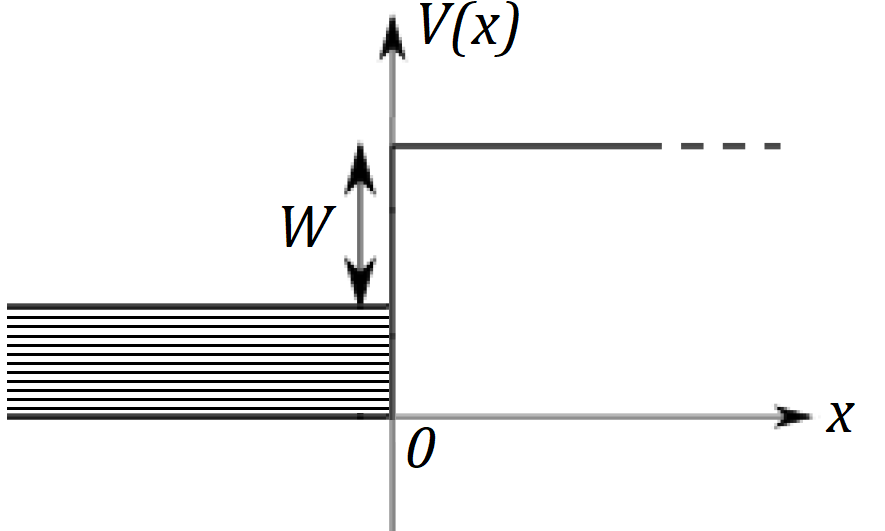
\includegraphics[width=0.5\textwidth]{immagini/cap_10/fig_10_9}
\end{center}
Nello stato fondamentale del metallo tutti i livelli di energia di singolo elettrone sono riempiti fino all'energia di Fermi. La differenza tra l'energia di Fermi e la cima della buca rappresenta l'energia necessaria per estrarre un elettrone dal metallo, ossia la \textbf{funzione lavoro} $w$.\\
Gli elettroni possono essere estratti dal metallo trasferendogli energia, o mediante fotoni o per riscaldamento.\\
Tuttavia \textbf{è} anche \textbf{possibile estrarre elettroni dal metallo senza fornire a questi alcuna energia} ma applicando un campo elettrico $\mathscr{E}$ all'esterno del metallo.\\
In questo caso infatti, il potenziale visto da un elettrone che si trova al livello di fermi cambia, per effetto del campo esterno, da $w+\varepsilon _F$ a $w+\varepsilon _F-e\mathscr{E}x$:
\vspace{.5cm}
\begin{minipage}{.5\textwidth}
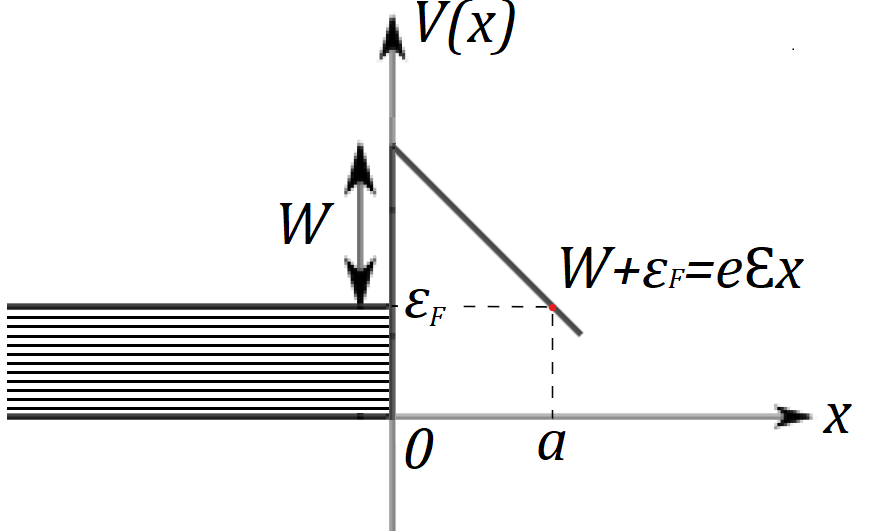
\includegraphics[width=.75\textwidth]{immagini/cap_10/fig_10_10.png}
\end{minipage}
\begin{minipage}{.5\textwidth}
\begin{equation}
w+\varepsilon _F-e\mathscr{E}a=\varepsilon _F ,
\end{equation}
\begin{equation}
a= w/(e\mathscr{E}) .
\end{equation}
\end{minipage}
L'elettrone può allore essere emesso per \textbf{effetto tunnel}.\\
la probabilità di emissione è:
\begin{equation}
T \approx \exp \left[-2 \int_{0} ^{a} dx\ \sqrt{\frac{2m}{\hbar ^2} (\underbrace{w+\varepsilon _F-e\mathscr{E}x}_{V(x)}-\underbrace{\varepsilon _F}_{E}})\right].
\end{equation}
Calcoliamo l'integrale:
\begin{equation}
\int _{0} ^{a} \left( w-e\mathscr{E}x \right) ^{1/2}= \left. -\frac{1}{e\mathscr{E}}\left( w-e\mathscr{E}x \right) ^{3/2}\frac{2}{3}\right| _0 ^a =\frac{2}{3}\frac{w^{3/2}}{e\mathscr{E}}.
\end{equation}
Pertanto:
\begin{equation}
T \approx \exp \left[-\frac{4}{3}\left(\frac{2m}{\hbar ^2}\right)^{1/2}\frac{w^{3/2}}{e\mathscr{E}}\right].
\end{equation}
\subsection{Decadimento alfa}
L'esperienza mostra che gli elementi di numero atomico $Z>81$ sono radioattivi, ossia decadono emettendo particelle $\alpha$ (nuclei di elio) o $\beta$ (elettroni) e trasformandosi così in altri elementi.\\
Indichiamo qui un \textbf{semplice modello per descrivere i decadimenti} $\mathbf{\alpha}$ le cui previsioni risultano in buon accordo con le osservazioni sperimentali.\\
In questo modello il decadimento del nucleo in una particella $\alpha$ ed un nucleo ``prodotto'' è descritto come l'emissione, per effetto tunnel, della particella $\alpha$ attraverso una barriera di potenziale causata dall'interazione coulombiana tra il nucleo prodotto e la particella $\alpha$:\\
\begin{center}
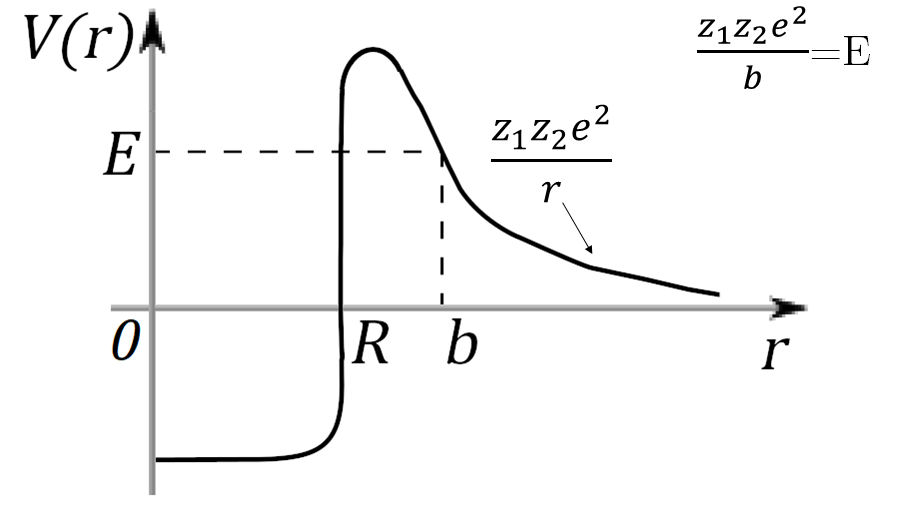
\includegraphics[width=.5\textwidth]{immagini/cap_10/fig_10_11.png}
\end{center}
Il raggio $R$ definisce le dimensioni del nucleo. Per $r<R$ la particella risente  del potenziale all'interno del nucleo, schematizzato da una buca. Per $r>R$ il potenziale è coulombiano: $V(r)=Z_1 Z_2 e^2/r$ dove $Z_1$ è la carica del nucleo prodotto e $Z_2=2$ la carica della particella $\alpha$.\\
Affinché il decadimento $\alpha$ (per effetto tunnel) possa avere luogo, la particella $\alpha$ all'interno del nucleo in questo modello deve avere energia $E$ positiva, ossia non deve trovarsi in uno stato legato.\\
La \textbf{probabilità di emissione} della particella $\alpha$ per effetto tunnel è:
\begin{equation}
T \approx \exp \left[ -2 \int _R ^b dr\ \sqrt{\frac{2m}{\hbar ^2}\left(\frac{Z_1 Z_2 e^2}{r}-E\right)}\right].
\end{equation}
Calcoliamo l'integrale:
\begin{eqnarray}
&\displaystyle{\int _R ^b dr\ \left(\frac{Z_1 Z_2 e^2}{r}-E\right)^{1/2}=\left(Z_1 Z_2 e^2\right)^{1/2}\int _R ^b \frac{dr}{\sqrt{r}}\left(1-\frac{Er}{Z_1 Z_2 e^2}\right)=}& \nonumber \\
&\displaystyle{=\left(Z_1 Z_2 e^2\right)^{1/2}\int _R ^b \frac{dr}{\sqrt{r}}\left(1-\frac{r}{b}\right)\overset{s=r/b}{=}}&\nonumber \\
&=\displaystyle{\left(Z_1 Z_2 e^2 b\right)^{1/2}\int _{R/b} ^1 ds\ s^{-1/2} (1-s)^{1/2}}.&
\end{eqnarray}
La piccolezza del raggio nucleare fa sì che risulta sempre valida con buona approssimazione la condizione
\begin{equation}
R\ll b \quad \Rightarrow \quad E \ll \frac{Z_1 Z_2 e^2}{r}
\end{equation}
Risulta pertanto possibile sostituire nel precedente integrale l'estremo inferiore di integrazione, $R/b$, con $0$. L'integrale si riduce quindi ad una costante adimensionale il cui valore,
\begin{equation}
\int _{0} ^1 ds\ s^{-1/2} (1-s)^{1/2}= \frac{\pi}{2},
\end{equation}
si può ottenere effettuando il cambio di variabile $s= \sin^2 \alpha$ (ma non è comunque rilevante per quanto segue).\\
Si trova pertanto:
\begin{eqnarray}
T&\approx & \exp \left[ -\frac{\pi}{(\hbar ^2 /2m)^{1/2}}\left(Z_1 Z_2 e^2 b\right)^{1/2}\right]= \nonumber \\
&=&\exp \left[ -\frac{\pi}{(\hbar ^2 /2m)^{1/2}}\frac{e^2}{\sqrt{E}}\right],
\end{eqnarray}
ossia
\begin{equation}
T \approx e^{-C\frac{Z_1}{\sqrt{E}}},
\end{equation}
che evidenzia la dipendenza della probabilità di decadimento dal numero atomico $Z_1$ del nucleo che decade e dall'energia $E=mv^2/2$ della particella $\alpha$ prodotta nel decadimento.\\
La probabilità di decadimento $\alpha$ del nucleo, T, è inversamente proporzionale alla \textbf{vita media} $\mathbf{\tau}$ del nucleo:
\begin{equation}
\tau=\frac{C'}{T}=e^{C'\frac{Z_1}{\sqrt{E}}},
\end{equation}
o, equivalentemente,
\begin{equation}
\log \tau = \log C' + \frac{C Z_1}{\sqrt{E}}.
\end{equation}
Questo andamento risulta ben confermato dalle misure sperimentali.
\section{Risoluzione dell'eq. di Schr\"{o}dinger per la barriera di potenziale in termini di f.d.o. simmetriche e anti-simmetriche}
L'equazione di Schr\"{o}dinger per la barrirea di potenziale può anche essere risolta, in modo conveniente, in termini di autofunzioni pari e dispari:
\begin{equation}
\psi _S (x) =
\begin{cases}
\displaystyle{e^{ikx} + A_s e^{-ikx} \qquad x<-a,}\\
B_S \cosh (\lambda x) \quad -a<x<a,\\
\displaystyle{e^{-ikx} + A_S e^{ikx} \qquad x>a.}
\end{cases}
\end{equation}
\begin{equation}
\psi _A (x) =
\begin{cases}
\displaystyle{e^{ikx} + A_A e^{-ikx} \qquad x<-a,}\\
B_A \sinh (\lambda x) \quad -a<x<a,\\
\displaystyle{-e^{-ikx} - A_A e^{ikx} \qquad x>a.}
\end{cases}
\end{equation}
Successivamente, una volta determinate le costanti $A$ e $B$ mediante le condizioni di continuità sulle f.d.o. e sulle derivate prime, si costruisce l'opportuna combinazione lineare per il problema dato:
\begin{equation}
\psi (x) =\frac{1}{2}\left(\psi _S (x) + \psi _A (x) \right) =
\begin{cases}
\displaystyle{e^{ikx} + \frac{1}{2}\left(A_S+A_A\right) e^{-ikx}} \\
\\
\displaystyle{\frac{1}{2}B_S \cosh (\lambda x )+ \frac{1}{2} B_A \sinh (\lambda x)} \\
\\
\displaystyle{\frac{1}{2}\left(A_S - A_A \right) e^{ikx}}
\end{cases}
\end{equation}
Vediamo, in particolare, che $\displaystyle{D=\frac{1}{2}\left( A_s - A_A \right)}$.\\
Calcoliamo il coefficiente $D$ utilizzando questo metodo.\\
Le condizioni di continuità per la f.d.o. simmetrica e per la sua derivata prima nel punto $x=a$ si scrivono
\begin{equation}
\begin{cases}
\displaystyle{B_S \cosh (\lambda a) = e^{-ika}+ A_S e^{ika}}\\
\displaystyle{\lambda B_S \sinh (\lambda a) = -ik e^{-ika}+ ikA_S e^{ika}}
\end{cases}
\label{eq:cap10_6}
\end{equation}
Per la simmetria della f.d.o. queste condizioni garantiscono anche la continuità della f.d.o. e della sua derivata nel punto $x=-a$.\\
Il sistema di equazioni (\ref{eq:cap10_6}) può essere facilmente risolto per $A_S$ moltiplicando la prima equazione per $\lambda \sinh (\lambda a)$, la seconda per $\cosh (\lambda a)$ e sottraendo l'una dall'altra:
\begin{equation}
\left(\lambda \sinh (\lambda a)+ ik\cosh (\lambda a) \right)e^{-ika}+ A_S \left(\lambda \sinh (\lambda a)-ik \cosh (\lambda a) \right)e^{ika}=0,
\end{equation}
da cui
\begin{equation}
A_S=-\frac{\lambda \sinh (\lambda a)+ik \cosh (\lambda a)}{\lambda \sinh (\lambda a)-ik \cosh (\lambda a)}e^{-2ika}.
\label{eq:cap10_7}
\end{equation}
La determinazione del coefficiente $A_A$ della f.d.o antisimmetrica procede in modo analogo. in questo caso le condizioni di continuità della f.d.o. e della sua derivata conducono al sistema
\begin{equation}
\begin{cases}
\displaystyle{B_A \sinh (\lambda a) = e^{-ika}- A_A e^{ika}}\\
\displaystyle{\lambda B_A \cosh (\lambda a) = ik e^{-ika}- ikA_A e^{ika}}
\end{cases}
\label{eq:cap10_8}
\end{equation}
Questo sistema differisce dal sistema (\ref{eq:cap10_6}) per lo scambio\\ $\sinh (\lambda a) \leftrightarrow -\cosh (\lambda a)$. Possiamo quindi scrivere direttamente dall'eq. (\ref{eq:cap10_7}) la soluzione per il coefficiente $A_A$:
\begin{equation}
A_A=-\frac{\lambda \cosh (\lambda a)+ik \sinh (\lambda a)}{\lambda \cosh (\lambda a)-ik \sinh (\lambda a)}e^{-2ika}.
\label{eq:cap10_9}
\end{equation}
dalle eq. (\ref{eq:cap10_7}) e (\ref{eq:cap10_9}) ricaviamo infine l'espressione cercata per il coefficiente $D$:
\begin{eqnarray}
D&=&\frac{1}{2}\left( A_S - A_A \right)= \nonumber \\
&=& -\frac{1}{2}e^{-2ika}\bigl[ \left( \lambda \sinh (\lambda a)+ ik \cosh (\lambda a )\right)\cdot\left( \lambda \cosh (\lambda a)- ik \sinh (\lambda a )\right)\nonumber \\ &-& \left( \lambda \cosh (\lambda a)+ ik \sinh (\lambda a )\right)\cdot \left( \lambda \sinh (\lambda a)- ik \cosh (\lambda a )\right)\bigr]/\bigl[ (\lambda \sinh (\lambda a)\nonumber\\
&-& ik\cosh (\lambda a ) \cdot (\lambda \cosh (\lambda a ) - ik \sinh (\lambda a ) \bigr]= \nonumber \\
&=& -\frac{1}{2}e^{-2ika} \frac{-2ik\lambda \sinh ^2 (\lambda a) + 2ik \lambda \cosh ^2 (\lambda a)}{ \left(\lambda ^2 - k^2 \right) \sinh (\lambda a ) \cosh (\lambda a) - ik\lambda \left(\sinh ^2 (\lambda a) + \cosh ^2 (\lambda a ) \right)}.\nonumber \\
\end{eqnarray}
Utilizzando le relazioni:
\begin{eqnarray}
& &\cosh ^2 x - \sinh ^2 x=1 \nonumber \\
& &\cosh ^2 x + \sinh ^2 x=\cosh 2x  \\
& &2 \cosh  x \sinh  x=\sinh 2x \nonumber 
\end{eqnarray}
possiamo riscrivere il coefficiente $D$ nella forma
\begin{equation}
D=\frac{2ik\lambda e^{-2ika}}{\left(k^2-\lambda^2\right)\sinh \left(2\lambda a\right)+2ik\lambda \cosh\left(2\lambda a\right)},
\end{equation}
che coincide con il risultato precedentemente ottenuto.
\section{Risoluzione dell'eq. di Schr\"{o}dinger per la barriera di potenziale nel limite $\mathbf{\lambda a \gg 1}$}
Consideriamo il sistema di equazioni (\ref{eq:cap10_10})e risolviamolo nel limite $\lambda a \gg 1$:
\begin{equation}
\begin{cases}
\displaystyle{2ik\ e^{-ika}=B\left( ik+\lambda\right)e^{-\lambda a} + C\left( ik-\lambda\right)e^{\lambda a}}\\
\\
\displaystyle{2ikA e^{ika}=B\left( ik-\lambda\right)e^{-\lambda a} + C\left( ik+\lambda\right)e^{\lambda a}}\\
\\
\displaystyle{B\left( ik+\lambda\right)e^{\lambda a} + C\left( ik-\lambda\right)e^{-\lambda a}}= 2ikD e^{ika}\\
\\
\displaystyle{B\left( ik-\lambda\right)e^{\lambda a} + C\left( ik+\lambda\right)e^{-\lambda a}}= 0\\
\end{cases}
\end{equation} 
dalla quarta equazione ricaviamo:
\begin{equation}
B=-\frac{(ik+\lambda)}{(ik-\lambda)}e^{-2 \lambda a } C,
\end{equation}
ossia $B$ è esponenzialmente piccolo rispetto a $C$.  nella prima equazione possiamo quindi trascurare il termine proporzionale a $Be^{-\lambda a}$ rispetto a quello proporzionale a $Ce^{\lambda a }$. Si ottiene in tal modo:
\begin{equation}
C= \frac{2ik}{(ik-\lambda)}e^{-ika}e^{-\lambda a},
\end{equation}
e dunque, combinando con la precedente equazione, anche
\begin{equation}
B=-\frac{2ik(ik+\lambda)}{(ik-\lambda)^2}e^{-ik a }e^{-3 \lambda a }.
\end{equation}
Possiamo ora ricavare il coefficiente $D$ utilizzando la terza delle equazioni del sistema. \\
In questa equazione i termini $Be^{\lambda a }$ e $Ce^{-\lambda a }$ sono dello stesso ordine di grandezza (entrambi proporzionali a $e^{-2\lambda a}$). Si ottiene dunque
\begin{eqnarray}
2ikDe^{-ika}&=& 2ike^{-ika}e^{-2\lambda a} \left[-\frac{(ik+\lambda)^2}{(ik-\lambda)^2}+1\right]= \nonumber \\
&=& 2ike^{-ika}e^{-2\lambda a}\frac{(ik-\lambda)^2-(ik+\lambda)^2}{(ik-\lambda)^2}= \nonumber \\
&=& 2ike^{-ika}e^{-2\lambda a}\left( -\frac{4ik\lambda}{(ik-\lambda)^2}\right),
\end{eqnarray}
da cui
\begin{equation}
D= -\frac{4ik\lambda}{(ik-\lambda)^2}e^{-2ika}e^{-2\lambda a}.
\end{equation}
il coefficiente di trasmissione risulta allora
\begin{equation}
T=|D|^2= \left(\frac{4k\lambda}{k^2+\lambda^2}\right) ^2 e^{-4\lambda a},
\end{equation}
in accordo con quanto ottenuto precedentemente nel limite $\lambda a \ll 1$.\\
Osserviamo infine che dalla seconda equazione del sistema, trascurando il termine $Be^{-\lambda a}$ (di $O(e^{-4\lambda a})$ ) rispetto al termine $Ce^{\lambda a}$ (di $O(1)$) si ottiene
\begin{equation}
A=\frac{(ik+\lambda)}{(ik-\lambda)}e^{-ika}\qquad \Rightarrow \qquad R=|A|^2=1+O(e^{-4\lambda a}).
\end{equation} %DEFINITIVO

\chapter[Oscillatore Armonico]{Oscillatore Armonico\footnote{S2.3, LL23, G5}}
Consideriamo una particella che compie piccole oscillazioni unidimensionale (il cosidetto \textbf{oscillatore armonico}). L'energia potenziale di tale particella è uguale a $\frac{1}{2}mw^2x^2$, dove $w$ rappresenta nella meccanica classica la frequenza propria delle oscillazioni. L'hamiltoniana dell'oscillatore è quindi:
\begin{equation}
H=\frac{p^2}{2m}+\frac{1}{2}mw^2x^2.
\label{eq:cap11_1}
\end{equation}
Poiché l'energia potenziale diventa infinita per $x=\pm \infty$, la particella può compiere soltanto un moto finito e, di conseguenza,  \textbf{tutto lo spettro} energetico dell'oscillatore \textbf{sarà discreto}.\\
 I livelli energetici dell'oscillatore armonico si possono determinare risolvendo \textbf{l'equazione di Schr\"{o}dinger indipendente dal tempo}:
\begin{equation}
H\psi= -\frac{\hbar^2}{2m}\frac{d^2\psi}{dx^2}+\frac{1}{2}mw^2x^2\psi=E\psi,
\end{equation}
con le condizioni al contorno:
\begin{equation}
\lim _{x \rightarrow \pm \infty} \psi(x)=0.
\end{equation}
Noi invece risolviamo il problema della determinazione dei livelli energetici, e dei relativi autostati, seguendo un elegante \textbf{metodo operatoria sviluppato da Dirac}.
 A tale scopo è conveniente in primo luogo introdurre degli operatori adimensionali, dividendo entrambe i membri dell'equazione (\ref{eq:cap11_1}) per $\hbar w$:
\begin{equation} \label{eq:cap11_2}
\frac{H}{\hbar w}=\frac{p^2}{2m\hbar w}+\frac{mw^2x^2}{2\hbar w}.
\end{equation}
Definendo allora:
\begin{eqnarray}  
	& &\hat{H}=\frac{H}{\hbar w},  \\
	& &\hat{p}=\frac{p}{\sqrt{\hbar w m}},  \\
	& &\hat{x}= \sqrt{\frac{mw}{\hbar}}x,
\end{eqnarray}
possiamo scrivere la precedente equazione nella forma:
\begin{equation}
\hat{H}=\frac{1}{2} (\hat{p}^2+\hat{x}^2).
\end{equation}
Calcoliamo il commutatore tra $\hat{p}$ e $\hat{x}$:
\begin{equation}
[\hat{p},\hat{x}]= \frac{1}{\sqrt{\hbar w m}} \sqrt{\frac{mw}{\hbar}} [p,x]=\frac{1}{\hbar}(-i\hbar),
\end{equation}
ossia:
\begin{equation}  \label{eq:cap11_3}
[\hat{p},\hat{x}]=-i.
\end{equation}
In termini degli operatori $\hat{p}$ ed $\hat{x}$ risulta poi conveniente definire due operatori non hermitiani:
\begin{equation} \label{eq:cap11_4}
\begin{split} 
	a=\frac{1}{\sqrt{2} } (\hat{x}+i\hat{p}), \\
	a^+=\frac{1}{\sqrt{2} } (\hat{x}-i\hat{p}),
\end{split} \end{equation}
o, più semplicemente:
\begin{equation} 
\begin{split}
	a=\sqrt{\frac{mw}{2\hbar}}(x+i \frac{p}{mw}), \\
	a^+=\sqrt{\frac{mw}{2\hbar}}(x-i \frac{p}{mw}).
\end{split}
\end{equation}
Facendo uso della regola di commutazione canonica (\ref{eq:cap11_3}) possiamo calcolare il commutatore tra $a$ e $a^+$:
\begin{equation}
[a,a^+]=\frac{1}{2} [\hat{x}+i\hat{p},\hat{x}-i\hat{p}]=\frac{1}{2}  \left( +i[\hat{p},\hat{x}]-i[\hat{x},\hat{p}]   \right ) = i[\hat{p},\hat{x}],
\end{equation}
e dunque:
\begin{equation}
\mathbf{[a,a^+]=1}.
\end{equation}
Esprimiamo l'operatore $\hat{H}$ in termini degli operatori $a$ e $a^+$. A tale scopo invertiamo le equazioni (\ref{eq:cap11_4}) per ottenere:
\begin{equation} \label{eq:cap11_5}
\begin{split} 
	\hat{x}=\frac{1}{\sqrt{2} } (a+a^+), \\
	\hat{p}=\frac{1}{\sqrt{2}i } (a-a^+).
\end{split}
\end{equation}
Si trova allora:
\begin{eqnarray}
	\hat{H} &=& \frac{1}{2} (\hat{p}^2+\hat{x}^2)=  \frac{1}{4} \left[ -(a-a^+)^2+(a+a^+)^2  \right]= \nonumber\\
	&= &\frac{1}{4} (aa^++a^+a)\cdot 2= \frac{1}{2}(aa^++a^+a)= \nonumber\\
	&=&\frac{1}{2}( [a,a^+]+2a^+a  )=\frac{1}{2}(1+2a^+a ),
\end{eqnarray}
ossia:
\begin{equation} 
\begin{split}
	\hat{H} =a^+a +\frac{1}{2}.
\end{split}
\end{equation}
Equivalentemente:
\begin{equation} \label{eq:cap11_6}
\begin{split}
	H =(a^+a+ \frac{1}{2}) \hbar w.
\end{split}
\end{equation}
Per comprendere il significato degli operatori $a$ e $a^+$ supponiamo di conoscere un autovalore $E_n$  dell'energia ed il corrispondente autostato $|n \rangle$:
\begin{equation}
H|n\rangle=E_n|n\rangle.
\end{equation}
Consideriamo quindi l'applicazione di H allo stato ottenuto applicando l'operatore $a$ ad $|n\rangle$:
\begin{equation}
Ha|n\rangle= [H,a]|n \rangle+aH|n\rangle=([H,a]+E_na)|n\rangle.
\end{equation}
Calcoliamo il commutatore [H,$a$]:
\begin{eqnarray}
	[H,a]&=&\hbar w[a^+a+\frac{1}{2},a]=\hbar w [a^+a,a]= \nonumber\\
	&=&\hbar w (a^+aa-aa^+a)=\hbar w[a^+,a]a=-\hbar wa.
\end{eqnarray}
Allora:
\begin{equation}
Ha|n\rangle=(E_n-\hbar w)a|n\rangle.
\end{equation}
Pertanto, se \textbf{$\mathbf{|n\rangle}$ è un autostato dell'hamiltoniana con autovalore $E_n$ allora anche $a|n\rangle$ è  un autostato dell'hamiltoniana con autosalone $E_n$-$\hbar w$. Per questa ragione l'operatore $a$ è anche detto \textit{operatore di distruzione}}.  \\
 Similmente possiamo considerare l'applicazione di H sullo stato $a^+|n\rangle$:
\begin{equation}
Ha^+|n\rangle= [H,a^+]|n\rangle+a^+H|n\rangle=([H,a^+]+E_na^+)|n\rangle.
\end{equation}
Il commutatore di H con $a^+$ risulta:
\begin{eqnarray}
	[H,a^+]&=&\hbar w[a^+a+\frac{1}{2},a^+]=\hbar w [a^+a,a^+]= \nonumber\\
	&=&\hbar w (a^+aa^+-a^+a^+a)=\hbar w a^+ [a,a^+]=\hbar wa^+,
\end{eqnarray}
o anche:
\begin{equation}
[H,a^+]=-[H,a]^+=\hbar w a^+.
\end{equation}
Allora:
\begin{equation}
Ha^+|n\rangle=(E_n+\hbar w)a^+|n\rangle,
\end{equation}
ossia se \textbf{$|n\rangle$ è un autostato dell'hamiltoniana con autovalore $E_n$ allora anche $a^+|n\rangle$ è  un autostato dell'hamiltoniana con autovalore $E_n$-$\hbar w$. Per questa ragione l'operatore $a^+$ è anche detto \textit{operatore di creazione}}. \\ 
 Questi risultati indicano che \textbf{i livelli di energia sono discreti e differiscono tra loro per un numero interno di unità $\hbar w$}.\\
 Un'altra importante osservazione è che gli autovalori dell'energia devono essere sempre positivi, ed anzi, più precisamente, maggiori od uguali di $\hbar w/2$. Si ha infatti:
\begin{eqnarray}
	E_n&=&\langle n|H|n \rangle= \hbar w \langle n|(a^+a+\frac{1}{2})|n\rangle= \nonumber \\
	&=&\hbar w (\langle n|(a^+a)|n\rangle+\frac{1}{2})=\hbar w (\langle n'|n'\rangle+\frac{1}{2}) \geq \frac{1}{2} \hbar w, 
\end{eqnarray}
giacché per qualunque ket $|n'\rangle$ si ha $\langle n'|n' \rangle\geq 0$ (e con $|n'\rangle= a|n\rangle$).
Deve dunque esistere uno \textbf{stato fondamentale}, il cui vettore di stato indicheremo con $|0\rangle$, la cui energia $E_0$ è maggiore o uguale di $\hbar w/2$. Poiché poi l'operatore $a$, se applicato ad un autostato, produce l'autostato di energia inferiore, deve valere la relazione:
\begin{equation}  \label{eq:cap11_7}
\mathbf{a|0\rangle=0}.
\end{equation}
 \textbf{L'energia del livello fondamentale} può essere ora facilmente calcolata:
\begin{equation}
H|0\rangle= \hbar w(a^+a+\frac{1}{2})|0\rangle= \frac{1}{2} \hbar w |0\rangle,
\end{equation}
ossia:
\begin{equation}
E_0=\frac{1}{2} \hbar w
\end{equation}
 I livelli di energia dell'oscillatore armonico risultano dunque dati da:
\begin{equation}
  \label{eq:cap11_8}
E_n=(n+\frac{1}{2}) \hbar w ,
\end{equation}
con   \textbf{n=0,1,2,...}

 L'equazione (\ref{eq:cap11_6}) implica che gli autostati $|n\rangle$ dell'hamiltoniana sono autostati simultanei dell'operatore $a^+a$. L'espressione (\ref{eq:cap11_8}) per gli autovalori dell'energia $E_n$ indica inoltre che i corrispondenti autovalori dell'operatore $a^+a$ sono i numeri interi n. Per tale ragione l'operatore hermitiano $a^+a$ è anche detto \textbf{operatore numero}:
\begin{equation}
\mathbf{N=a^+a},
\end{equation}
e si ha:
\begin{equation}
\mathbf{N|n\rangle=n|n\rangle}.
\end{equation}
\\\\
 Discutiamo ora come gli autostati $|n\rangle$ dell'hailtoniana possono essere costruiti a partire dall'autostato $|0\rangle$ corrispondente allo stato fondamentale dell'oscillatore.
 Il ruolo degli operatori $a$ e $a^+$ come operatori di distruzione e costruzione rispettivamente implica che gli stati $a|n\rangle$ ed $a^+|n\rangle$ coincidono, a meno di una costante di normalizzazione, con gli autostati $|n-1\rangle$ ed $|n+1\rangle$. Possiamo pertanto scrivere:
\begin{equation}
\begin{cases}
a|n\rangle=c_n|n-1\rangle,\\
a^+|n-1\rangle=d_n|n\rangle.
\end{cases}.
\end{equation}
 Per ricavare le costanti $c_n$ e $d_n$ osserviamo innanzitutto che:
\begin{equation}
c_n=\langle n-1|a|n\rangle=\langle n|a^+|n-1\rangle^*=d_n^*.
\end{equation}
 Inoltre, applicando l'operatore numero allo stato $|n\rangle$ troviamo:
\begin{equation}
N|n\rangle=n|n\rangle=a^+a|n\rangle=c_na^+|n-1\rangle=c_nd_n|n\rangle=|c_n|^2|n\rangle,
\end{equation}
ossia:
\begin{equation}
|c_n|^2=n.
\end{equation}
Scegliendo per convenzione $c_n$ reale e positivo (tale scelta essendo sempre possibile giacché i vettori di stato sono definiti a meno di un fattore di fase arbitrario) vediamo allora che $c_n=\sqrt{n}$. In definitiva abbiamo dimostrato le relazioni:
\begin{equation} \label{eq:cap11_9}
\begin{cases}
a|n\rangle= \sqrt{n} |n-1\rangle, \\
a^+|n-1\rangle=\sqrt{n}|n\rangle.
\end{cases}
\end{equation}
Queste relazioni consentono in particolare di costruire tutti gli autostati dell'hamiltoniana applicando in successione l'operatore $a^+$ allo stato fondamentale $|0\rangle$. Otteniamo:\\\\
\begin{eqnarray} \label{eq:cap11_10}  %non so come mandare tutto a sx
& &|1\rangle=a^+|0\rangle \nonumber \\
& &|2\rangle=\frac{1}{\sqrt{2}}a^+|1\rangle=\frac{1}{\sqrt{2}}(a^+)^2|0\rangle \nonumber \\
& &|3\rangle= \frac{1}{\sqrt{3}}a^+|2\rangle=\frac{1}{\sqrt{3!}}(a^+)^3|0\rangle   \\
& &... \nonumber\\
& &|n\rangle=\frac{1}{\sqrt{n!}}(a^+)^n|0\rangle \nonumber
\end{eqnarray}



 Il metodo operatoriale di Dirac consente anche di ricavare le \textbf{f.d.o nello spazio delle coordinate corrispondenti agli autostati dell'energia.}\\
 Consideriamo in primo luogo lo stato fondamentale definito dall'equazione (\ref{eq:cap11_7}). Moltiplicando a sinistra questa equazione per il $\langle x'|$ troviamo:
\begin{equation}
\langle x'|a|0 \rangle= \sqrt{\frac{mw}{2\hbar}}\langle x'|(x+\frac{ip}{mw})|0 \rangle=0.
\end{equation}
Ricordando le espressioni degli operatori x e p nella rappresentazione delle coordinate, otteniamo l'equazione:
\begin{equation} \label{eq:cap11_12}
\sqrt{\frac{mw}{2\hbar}}(x'+\frac{\hbar}{mw}\frac{d}{dx'})\psi_0(x')=0,
\end{equation}
dove si è indicata con:
\begin{equation}
\psi_0(x')=\langle x'|0 \rangle.
\end{equation}
l'autofunzione corrispondente allo stato fondamentale dell'oscillatore. \\
Ponendo:
\begin{equation}
x_0=\sqrt{\frac{\hbar}{mw}} \qquad \textrm{e} \qquad \xi=\frac{x'}{x_0},
\end{equation}
si può riscrivere l'equazione (\ref{eq:cap11_12}) nella forma:
\begin{equation}  \label{eq:cap11_13}
a\psi_o(\xi)=\frac{1}{\sqrt{2}}(\xi+\frac{d}{d\xi})\psi_0(\xi)=0.
\end{equation}
Per inciso vediamo che \textbf{nella rappresentazione delle coordinate, in termini della variabile adimensionale $\xi=x/x_0$, gli operatori di creazione e distruzione si esprimono come}:
\begin{equation}    \label{eq:cap11_14}
\begin{split}
	a=\frac{1}{\sqrt{2}} (\xi+\frac{d}{d\xi}) \\
	a^+=\frac{1}{\sqrt{2}} (\xi-\frac{d}{d\xi}) 
\end{split} \end{equation}
 L'equazione (\ref{eq:cap11_13}) si integra facilmente per separazione di variabili:
\begin{equation}
\frac{d\psi_0}{d\xi}=-\xi\psi_0 \rightarrow \frac{d\psi}{\psi_0}=-\xi d\xi \rightarrow ln\psi_0=-\frac{\xi^2}{2}+cost,
\end{equation}
ossia:
\begin{equation}
\psi_0(\xi)=Ce^{-\xi^2/2}.
\end{equation}
La costante C è determinata dalla \textbf{condizione di normalizzazione}:
\begin{equation}
\langle 0|0 \rangle=\int_{-\infty}^{+\infty} dx' \langle 0|x'\rangle\langle x'|0 \rangle=\int_{-\infty}^{+\infty} dx' |\psi_0(x')|^2=1.
\end{equation}
Troviamo in tal modo:
\begin{equation}
\int_{-\infty}^{+\infty} dx' |\psi_0(x')|^2=|C|^2x_0\int_{-\infty}^{+\infty} d\xi e^{-\xi^2}=|C|^2 x_0 \sqrt{\pi}=1,
\end{equation}
da cui, scegliendo C reale e positivo:
\begin{equation}
C=\frac{1}{\pi^{{1}/{4}}} \sqrt{x_0}.
\end{equation}
Pertanto \textbf{l'autofunzione normalizzata corrispondente allo stato fondamentale dell'oscillatore armonico è}:
\begin{equation}
\psi_0=\left( \frac{1}{\pi^{{1}/{4}}}  \right) e^{-\xi^2/2}, \qquad \qquad \xi=\frac{x}{x_0}.
\end{equation}
 Le equazioni (\ref{eq:cap11_10}) consentono poi di valutare le \textbf{autofunzioni dell'energia per gli stati eccitati.} Per la generica f.d.o dell'autostato $|n\rangle$ possiamo scrivere:
\begin{equation}
\psi_n(x')=\langle x'|n \rangle=\frac{1}{\sqrt{n!}}\langle x'|(a^+)^n|0 \rangle,
\end{equation}
da cui, utilizzando la rappresentazione espressa nell'equazione (\ref{eq:cap11_14}) per l'operatore $a^+$ ricaviamo:
\begin{equation} \label{eq:cap11_15}
\begin{split}
	\psi_n(\xi)=\frac{1}{\sqrt{2^nn!}}(\xi-\frac{d}{d\xi})^n \psi_0({\xi})=\\
	=\frac{1}{\pi^{1/4}\sqrt{2^nx_0n!}}(\xi-\frac{d}{d\xi})^n e^{-\xi^2/2}.
\end{split} \end{equation}

 Le funzioni H$_n({\xi})$ definite dall'equazione:
\begin{equation}
(\xi-\frac{d}{d\xi})^n e^{-\xi^2/2}=H_n(\xi)e^{-\xi^2/2},
\end{equation}
sono dei polinomi di grado $n$ in $\xi$ contenenti potenze della stessa parità del numero $n$, Queste funzioni dono dette \textbf{polinomi di Hermite.} L'equazione (\ref{eq:cap11_15}) si scrive allora, in termini di questi polinomi:
\begin{equation}
\psi_n(\xi)=\frac{1}{\pi^{1/4}\sqrt{2^nx_0n!}} H_n(\xi)e^{-\xi^2/2}.
\end{equation}

\newpage
\begin{figure}[htbp]
\begin{center}
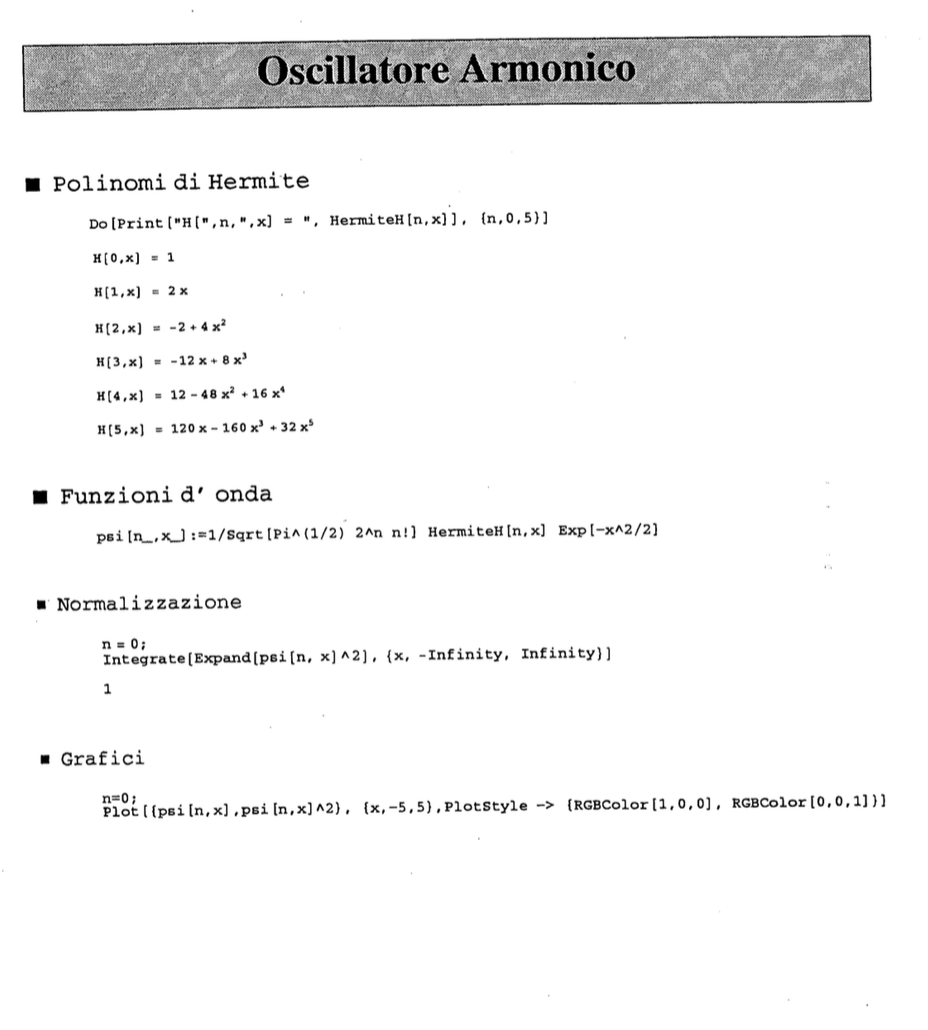
\includegraphics[width=\textwidth]{immagini/cap_11/polHer1.png}
\end{center}
\end{figure}

\begin{figure}[htbp]
\begin{center}
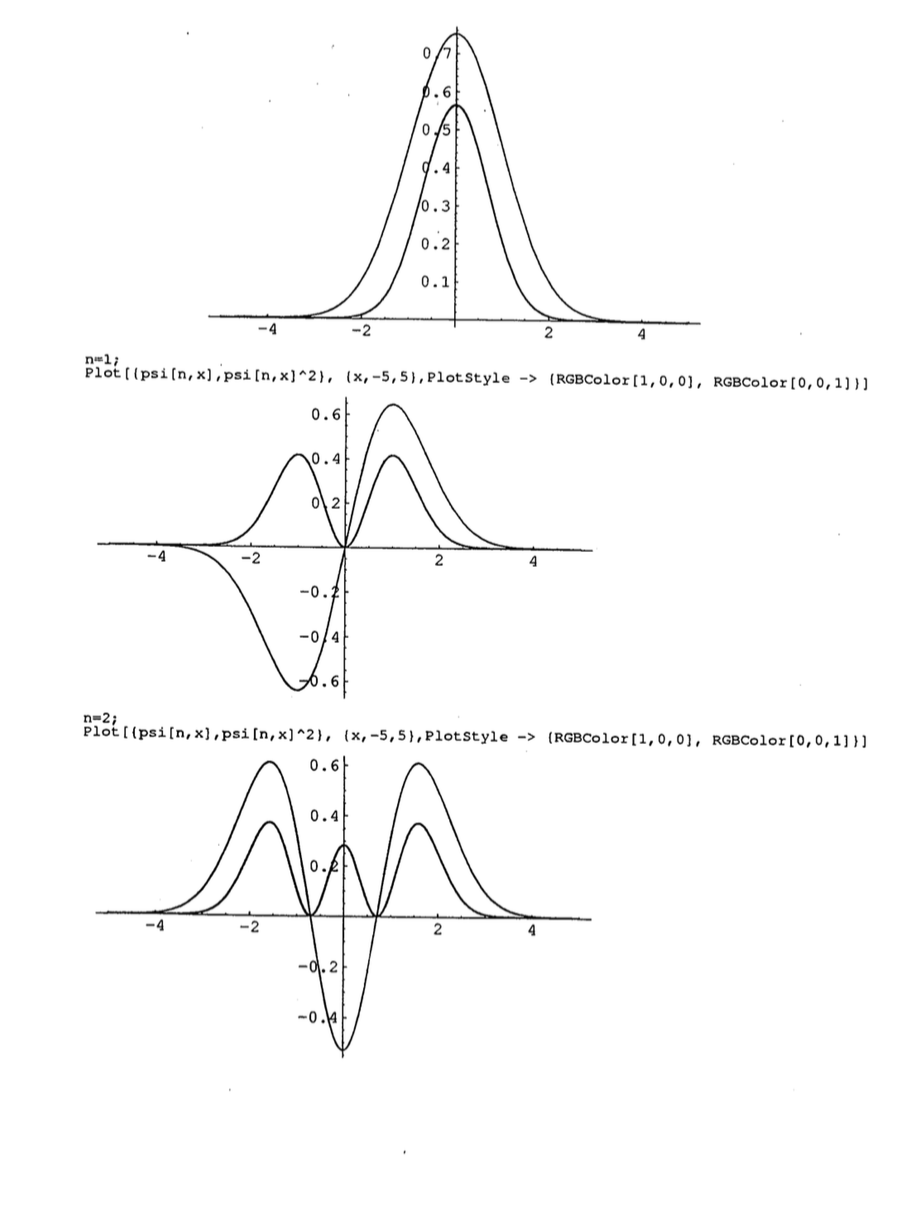
\includegraphics[width=\textwidth]{immagini/cap_11/polHer2.png}
\end{center}
\end{figure}
 %DEFINITIVO
\chapter[Simmetrie e Leggi di Conservazione]{Simmetrie e Leggi di\\ Conservazione} 
\section{Derivata di un operatore rispetto al tempo} 

\textbf{Il concetto di derivata di una grandezza fisica rispetto al tempo non può essere definito in meccanica quantistica nel senso che esso ha in meccanica classica. Infatti, la definizione della derivata in meccanica classica è legata alla considerazione dei valori della grandezza in due istanti vicini ma differenti. Nella meccanica quantistica, invece, una grandezza avente un valore determinato in un certo istante non ha, in generale, valore determinato negli istanti successivi.} 

In altri termini, se il vettore di stato del sistema considerato è un autostato di una determinata osservabile ad un certo istante, negli istanti successivi il vettore di stato non sarà più, in generale, autoscatto della stessa osservabile.

Dunque, il concetto di derivata rispetto al tempo deve essere definito in meccanica quantistica in modo diverso.
\textbf{\'E naturale definire la derivata $\mathbf{dA/dt}$ di A come grandezza il cui valore medio è uguale alla derivata rispetto al tempo del valor medio $\mathbf{\langle A \rangle} $.
Si ha dunque, per definizione}:

\begin{equation}
\langle \frac{dA}{dt} \rangle = \frac{d}{dt} \langle A \rangle .
\end{equation}

Partendo da questa definizione non è difficile ottenere l'espressione dell'operatore quantistico $dA/dt$

\begin{eqnarray}
\label{eq:cap12_1}
\langle \frac{dA}{dt} \rangle &=& \langle \alpha,t| \frac{dA}{dt}| \alpha,t \rangle = \frac{d}{dt} \langle A \rangle = \frac{d}{dt} \langle \alpha ,t |A| \alpha ,t\rangle= \nonumber\\
&=&(\frac{\partial }{\partial{t}}\langle \alpha,t|) A|\alpha,t \rangle + \langle \alpha,t| \frac{\partial A}{\partial{t}}|\alpha,t \rangle + \\
& &+\langle\alpha,t|A (\frac{\partial }{\partial{t}}|\alpha,t\rangle).\nonumber
\end{eqnarray} 

In questa espressione $\frac{\partial A}{\partial{t}}$ è un operatore dedotto per derivazione dell'operatore A rispetto al tempo, dal quale quest'ultimo può dipendere come da un parametro.

Utilizzando l'equazione di Schr\"{o}dinger per il ket $|\alpha,t\rangle$ e per il bra corrispondente,   $\langle\alpha,t|$ :

\begin{equation}
\begin{cases}
\displaystyle{i\hbar\frac{\partial }{\partial{t}}|\alpha,t\rangle= H|\alpha,t\rangle }\\
\\
\displaystyle{-i\hbar\frac{\partial }{\partial{t}}\langle\alpha,t|= \langle\alpha,t|H } 
\end{cases}
\end{equation}

otteniamo dall'eq. (\ref{eq:cap12_1})

\begin{eqnarray}
\langle\frac{dA}{dt} \rangle &=& \frac{i}{\hbar} \langle\alpha,t|HA|\alpha,t\rangle + \langle \alpha,t|\frac{\partial A}{\partial{t}}|\alpha,t \rangle + \nonumber \\
& &-\frac{i}{\hbar} \langle \alpha,t|AH|\alpha,t\rangle=  \nonumber\\
&=& \langle \alpha,t| (\frac{\partial A}{\partial{t}} + \frac{i}{\hbar}[H,A] ) |\alpha,t\rangle .
\end{eqnarray}


Per definizione di valore medio, l'espressione tra parentesi rappresenta l'operatore cercato $dA/dt$ :

\begin{equation} \label{eq:cap12_2}
\frac{dA}{dt}= \frac{\partial A}{\partial{t}}+ \frac{i}{\hbar}[H,A].
\end{equation}

È istruttivo confrontare questo risultato con l'equazione del moto classico nella forma di parentesi di Poisson. \textbf{In meccanica classica}, per la derivata totale rispetto al tempo di una grandezza $f$, che è funzione delle coordinate e dei momenti generalizzati $q_i$ e $p_i$ del sistema, si ha:

 \begin{equation}
\frac{df}{dt}= \frac{\partial f}{\partial{t}} + \sum_{i}^{}{(\frac{\partial H}{\partial{p_i}}\frac{\partial f}{\partial{q_i}} - \frac{\partial H}{\partial{q_i}}\frac{\partial f}{\partial{p_i}}} )=
\frac{\partial f}{\partial{t}}+ \{H,f\}.
\end{equation}

Nuovamente riscontriamo che la regola di corrispondenza di Dirac 

\begin{equation}
\{ \quad,\quad   \}_{classica}  \leftrightarrow \frac{i}{\hbar} [ \quad, \quad]
\end{equation}

porta all'equazione corretta in meccanica quantistica.
È bene sottolineare, tuttavia, come l'eq (\ref{eq:cap12_2})risulti valida anche quando la grandezza A non ha analogo classico.\\
Una classe molto importante di grandezze fisiche è costituita da \textbf{quelle grandezze i cui operatori non dipendono esplicitamente dal tempo e che, inoltre, commutano con l'hamiltoniano} in modo tale che 

\begin{equation}
\frac{dA}{dt}= \frac{\partial A}{\partial{t}} + \frac{i}{\hbar}[H,A]=0.
\end{equation}

Tali grandezze si chiamano \textbf{conservative}.

Per le grandezze conservative 
\begin{equation} 
\langle \frac{dA}{dt}\rangle= \frac{d}{dt}\langle A \rangle =0,
\end{equation}
cioè 
\begin{equation}
\langle A \rangle= costante.
\end{equation}

In altri termini \textbf{il valore medio della grandezza resta costante nel tempo}. Si può ugualmente affermare che \textbf{se, nello stato dato, la grandezza A ha un valore determinato (cioè se lo stato è un autostato dell'operatore A) essa avrà anche negli istanti successivi un valore determinato ed esattamente lo stesso.}

\textbf{L'hamiltoniano di un sistema isolato (nonchè di un sistema che si trova in un campo esteso costante e non variabile) non può contenere il tempo esplicitamente.} Ciò risulta dal fatto che tutti gli istanti sono equivalenti relativamente a tale sistema fisico. Pertanto, per un tale sistema  
\begin{equation}
\frac{\partial H}{\partial{t}}=0.
\end{equation}

D'altra parte, poiché ogni operatore, come è ovvio, commuta con se stesso possiamo calcolare che \textbf{l'energia di un sistema che non si trova in un campo esteso variabile si conserva}:
\begin{equation}
\frac{dH}{dt}=0.
\end{equation}

Pertanto \textbf{in meccanica quantistica la legge di conservazione dell'energia significa che, se nello stato dato l'energia ha un valore determinato, questo valore resterà nel tempo}.

\section[Simmetrie e leggi di conservazione  in meccanica quantistica]{Simmetrie e leggi di conservazione  in meccanica quantistica\footnote{S22, 4.1 }} 

La legge di conservazione dell'energia, discussa nel paragrafo precedente, rappresenta un esempio specifico di \textbf{connessione tra simmetrie e leggi di conservazione}. Questa legge può essere infatti enunciata dicendo che,se un sistema fisico è invariante rispetto a traslazioni temporali, allora il corrispondente generatore della trasformazione, ossia l'hamiltoniano $H$, è una quantità conservata.

\textbf{Così come in meccanica classica, anche in meccanica quantistica la connessione tra simmetria e leggi di conservazione può essere stabilita in forma del tutto generale}.

Per discutere questa connessione consideriamo una generica trasformazione che Ú rappresentata, in meccanica quantistica, da un operatore unitario agente sui vettori di stato:

\begin{equation}\label{eq:cap12_3}
|\alpha \rangle \rightarrow\textbf{U}|\alpha \rangle.
\end{equation}

Possiamo pensare che $\textbf{U}$ rappresenti l'operatore di traslazione spaziale $T(d\vec{x})$ oppure l'operatore di evoluzione temporale, $\textbf{U}(t,t_0)$.

Consideriamo come cambia, per effetto della trasformazione, un generico elemento di matrice di un operatore \textbf{X} tra due stati $|\alpha \rangle$ e $|\beta\rangle$ :

\begin{equation}
\langle \beta|\textbf{X}|\alpha \rangle   \mapsto    \langle \beta |\textbf{U}^+\textbf{X}\textbf{U}|\alpha \rangle.
\end{equation}

Vediamo allora che la trasformazione può essere pensata o come una trasformazione (\ref{eq:cap12_3})  sui vettori di stato, che lascia gli operatori invariati, o come trasformazione sugli operatori:

\begin{equation}
\label{eq:cap12_4}
\textbf{X}\mapsto \textbf{U}^+ \textbf{X}\textbf{U},
\end{equation}
lasciando invariati i vettori di stato. Formalmente i due approcci sono completamente equivalenti.

Come esempio discutiamo il caso di una traslazione spaziale infinitesima operata dall'operatore $T(d\vec{x}^{'})$.
Nell'approccio utilizzato in precedenza, la trasformazione era pensata come una trasformazione sui vettori di stato che lascia invariati gli operatori.

Così ad esempio:

\begin{eqnarray}
  &|\alpha \rangle \rightarrow (1- \frac{i}{\hbar}\vec{p}\cdot d\vec{x}^{'}) |\alpha \rangle &  \\
	\nonumber \\
 & \vec{X}\rightarrow \vec{X}  & 
\end{eqnarray}

Tuttavia possiamo considerare la trasformazione come una trasformazione degli operatori, che lascia invariati i vettori di stato:

\begin{eqnarray}
	|\alpha \rangle &\rightarrow & |\alpha \rangle \\
	\vec{X} &\rightarrow& (1+ \frac{i}{\hbar} \vec{p} d\vec{x}^{'}) \vec{X} (1-\frac{i}{\hbar} \vec{p} d\vec{X}) \approx \nonumber\\
	& &\approx \vec{X}+ \frac{i}{\hbar}[\vec{p} d\vec{x}^{'},\vec{x}]= \nonumber  \\
	&=&\vec{X}+ d\vec{X}^{'}
\end{eqnarray}

È immediato mostrare come entrambi gli approcci portano allo stesso risultato per il valore di aspettazione di $\vec{x}$:

\begin{equation}
\langle \vec{x} \rangle  \mapsto \langle \vec{x}\rangle + \langle d\vec{x}^{'} \rangle.
\end{equation}
Nel discutere la connessione tra simmetrie e leggi di conservazione è conveniente considerare le trasformazioni come agenti sugli operatori.

\textbf{Consideriamo allora una generica trasformazione operata dall'operatore unitario $\textbf{U}$ e supponiamo che il sistema fisico considerato sia invariate rispetto a tale trasformazione, ossia che la trasformazione rappresenti una simmetria del sistema.
In particolare, allora, dovrà risultare invariate per tale trasformazione l'hamiltoniano H del sistema, che ne descrive la dinamica}. Per quanto discusso questo comporta

\begin{equation}
\textbf{U}^+H\textbf{U}= H,
\end{equation}

o, equivalentemente 

\begin{equation}\label{eq:cap12_5}
[H,\textbf{U}]=0.
\end{equation}

Se consideriamo una \textbf{trasformazione infinitesima}, sappiamo che l'operatore unitario $\textbf{U}$ può essere scritto nella forma 

\begin{equation}
\textbf{U}= 1- \frac{i\epsilon}{\hbar}G
\end{equation}

dove G è il generatore hamiltoniano della trasformazione considerata. In questo caso l'equazione (\ref{eq:cap12_5}) equivale a 

\begin{equation} 
[H,G]=0.
\end{equation}

Per l'eq. (\ref{eq:cap12_4}) si ha allora

\begin{equation}
\frac{dG}{dt}=0,
\end{equation}

e quindi \textbf{G è una costante del moto}. Questo risultato stabilisce la connessione tra simmetrie e leggi di conservazione nella meccanica quantistica.

Considero ad esempio un \textbf{sistema isolato soggetto a campi esterni}. Poichè tutte le posizioni di tale sistema in blocco sono equivalenti nello spazio, si può affermare che l'hamiltoniano del sistema non cambia in uno spostamento arbitrario del sistema. In altri termini l'hamiltoniano commuta con l'operazione di traslazione

\begin{equation}
[H,T (d\vec{x}^{'})]=0.
\end{equation}

Ma questo equivale a dire che \textbf{l'hamiltoniano commuta con l'operatore impulso $\vec{p}$} del sistema è una quantità conservata:

\begin{equation}
\frac{d\vec{p}}{dt}=0.
\end{equation}

Possiamo quindi affermare che \textbf{in meccanica quantistica,come in meccanica classica, la legge di conservazione dell'impulso di un sistema isolato è una diretta conseguenza dell'omogeneità dello spazio.}

In seguito mostreremo che, \textbf{come conseguenza dell'invariata rispetto a rotazioni spaziali di un sistema isolato non soggetto a campi esterni, si conserva in meccanica quantistica, come in meccanica classica, il momento angolare del sistema. La legge di conservazione del momento angolare è dunque una conseguenza dell'isotropia dello spazio.}

\textbf{L'invarianza di un sistema isolato, o di un sistema soggetto a campi esterni variabili nel tempo, rispetto a traslazioni temporali è conseguenza dell'omogeneità del tempo. La conservazione dell'energia è dunque una diretta conseguenza di tale simmetria}.

Sin qui abbiamo discusso in particolare il caso delle \textbf{simmetrie continue}, ossia delle simmetrie associate a trasformazioni che possano essere ottenute applicando successivamente trasformazioni infinitesime.
Esistono tuttavia trasformazioni che non godono di questa proprietà, e che sono associate a cosiddette \textbf{simmetrie discrete}. In questo caso non esiste alcun generatore hamiltoniano associato alla trasformazione e dunque potrebbe non esistere alcuna osservabile corrispondente ad una quantità conservata.

Per alcune simmetrie discrete, tuttavia, lo stesso operatore unitario \textbf{U} che opera la trasformazione può essere al tempo stesso, un operatore hermitiano. In vista dell'eq (\ref{eq:cap12_5}), allora l'operatore \textbf{U} corrisponde ad una quantità osservabile conservata. Questo è il caso, ad esempio, della \textbf{trasformazione di inversione spaziale o parità}. Abbiamo già discusso come la parità sia infatti una quantità conservata per sistemi in cui il campo di forze estese è descritto da un potenziale simmetrico rispetto ad inversione degli assi.

\section[Teorema di Ehrenfest]{Teorema di Ehrenfest\footnote{S2.2, LL19}}

Consideriamo l'operatore di Hamilton per una particella:

\begin{equation}
H= \frac{\vec{p}^2}{2m} + \textbf{V}(\vec{x}).
\end{equation}

Calcoliamo l'operatore $d\vec{x}/dt$. Poichè l'operatore di posizione $\vec{x}$ non dipende esplicitamente dal tempo, in virtù dell'eq (\ref{eq:cap12_4}) si ha:

\begin{equation}
\frac{d\vec{x}}{dt}= \frac{i}{\hbar}[H,\vec{x}].
\end{equation}

L'unico operatore tra i componenti di H che non commuta con l'operatore di posizione è $\vec{p}^2$. Si ha allora 

\begin{equation}
\frac{dx_i}{dt}=\frac{i}{\hbar} \left[ \frac{p_i^2}{2m},x_i \right]=\frac{i}{2m\hbar}(p_i^2x_i-x_ip_i^2)=\frac{p_i}{m},
\end{equation}
con $[p^2,x]=p[p,x]+[p,x]p=-2i\hbar$. Si ha:
\begin{equation}
   	\label{eq:cap12_6}
	\frac{d\vec{x}}{dt}=\frac{\vec{p}}{m}.
\end{equation}
Calcoliamo ora l'operatore $\displaystyle{\frac{d\vec{p}}{dt}}$. Otteniamo facilmente il risultato cercato utilizzando per gli operatori la loro espressione nella rappresentazione delle coordinate:\\
\begin{eqnarray}
	\frac{d\vec{p}}{dt}&=&\frac{i}{\hbar}[\vec{H},\vec{p}]=\frac{i}{\hbar}[V(\vec{x}),\vec{p}]= \nonumber\\
	&=&\frac{i}{\hbar}[V(\vec{x}),-i\hbar\vec{\nabla}]=(V(\vec{x})\vec{\nabla}-\vec{\nabla}V(\vec{x}))= \nonumber \\
	&=&V(\vec{x})\vec{\nabla}-(\vec{\nabla}V(\vec{x}))-V	\vec{x}\vec{\nabla},
\end{eqnarray}
ossia:

\begin{equation}
\label{eq:cap12_7}
\frac{d\vec{p}}{dt}=-\vec{\nabla}V(\vec{x}).
\end{equation}
Le due equazioni, (\ref{eq:cap12_6}) e (\ref{eq:cap12_7}), possono essere combinate insieme per ottenere:\\
\begin{equation}
m\frac{d^2\vec{x}}{dt^2}=\frac{d\vec{p}}{dt}=-\vec{\nabla}V(\vec{x}),
\end{equation}

che esprimono, in forma operatoriale, la legge di Newton. Questo risultato è noto come \textbf{Teorema di Ehrenfest}. 
 %DEFINITIVO
\chapter[Rappresentazioni di Schrödinger e di Heisenberg]{Rappresentazioni\\ di Schrödinger e di\\ Heisenberg ed equazioni\\ del moto di Heisenberg\footnote{S22, LL13}}

Nel discutere la dinamica in meccanica quantistica, abbiamo considerato come i vettori di stato evolvono nel tempo secondo l'equazione di Schrödinger. Questo significa che abbiamo considerato la trasformazione di evoluzione temporale come una trasformazione applicata ai vettori di stato, che lascia invariati gli operatori. Questo approccio è noto come \textbf{rappresentazione~di~Schr\"{o}dinger}.\\
In accordo con la precedente discussione generale, possiamo considerare la trasformazione di evoluzione temporale nell'approccio alternativo, e completamente equivalente, secondo cui la trasformazione è applicata agli operatori, mentre i vettori di stato restano invariati nel tempo. Questo approccio è noto come $\textbf{rappresentazione~di~Heisenberg}$.\\
\\
\noindent Consideriamo allora l'operatore di evoluzione temporale $U(t, t_0)$ e poniamo per semplicità $t_0 = 0$ :
 
\begin{equation}
U(t) \equiv U(t,t_0 = 0) = e^{-\frac{i}{\hbar}Ht}.
\end{equation}
\\
\noindent Nella rappresentazione di Schrödinger gli stati evolvono nel tempo e gli operatori restano invariati:

\begin{align}
\ket{\alpha, t_0 = 0}_S &\rightarrow \ket{\alpha, t}_S = U(t) \ket{\alpha, t=0}_S \nonumber \\
A^{(S)} &\rightarrow A^{(S)}.
\end{align}
\\
\noindent Nella rappresentazione di Heisenberg, viceversa, gli stati restano invariati e gli operatori evolvono nel tempo:

\begin{align}
&\ket{\alpha}_H \rightarrow \ket{\alpha}_H, \\ \nonumber
&A^{(H)}(t_0 = 0) \rightarrow A^{(H)}(t) = U^\textbf{+}(t)A^{(H)}(t_0 = 0)U(t).
\end{align}
\\
\noindent Per definizione i vettori di stato e gli operatori coincidono nelle rappresentazioni di Schrödinger e di Heisenberg al tempo $t_0 = 0$ :

\begin{align}
\ket{\alpha}_H = \ket{\alpha, t_0 = 0}_S, \\ \nonumber
A^{(H)}(t_0 = 0) = A^{(S)}.
\end{align}
\\
\noindent Il valore di aspettazione di un generico operatore $A$ su qualunque stato $\ket{\alpha}$ è ovviamente identico nelle due rappresentazioni:

\begin{eqnarray}
~_S\braket{\alpha,t|A^{(S)}|\alpha,t}_S &=& _S\langle \alpha, t_0=0\vert U^\textbf{+}(t) A^{(S)}U(t)\vert\alpha,t_0=0\rangle _S \nonumber \\
&=&~_H\braket{\alpha|A^{(H)}(t)|\alpha}_H.
\end{eqnarray}
\\
\noindent Così come nella rappresentazione di Schrödinger l'evoluzione temporale degli stati è definita dall'equazione di Schrödinger, in modo analogo è possibile derivare, nella rappresentazione di Heisenberg, un'equazione fondamentale che definisce l'evoluzione temporale degli operatori. Questa equazione può essere derivata derivando rispetto al tempo l'operatore $A^{(H)}(t)$ nella rappresentazione di Heisenberg:

\begin{align}
& \frac{dA^{(H)}(t)}{dt} = \frac{d}{dt}\left[U^\textbf{+}(t) A^{(H)}(t_0=0)U(t)\right] = \nonumber \\
&= \frac{\partial U^\textbf{+}(t)}{dt} A^{(H)}(t_0=0) U(t) + U^\textbf{+}(t) A^{(H)}(t_0=0) \frac{\partial U(t)}{dt} = \nonumber \\
&= \frac{i}{\hbar} H U^\textbf{+}(t) A^{(H)}(t_0=0) U(t) + U^\textbf{+}(t) A^{(H)}(t_0=0) \left(-\frac{i}{h}\right) H U(t) = \nonumber \\
&= \frac{i}{\hbar} H A^{(H)}(t) - \frac{i}{h} A^{(H)}(t) H,
\end{align}

\noindent dove si è supposto che l'operatore $A$, così come l'hamiltoniana $H$, non dipendano esplicitamente (ossia parametricamente) dal tempo. Dunque:

\begin{equation} \label{eq:cap13_1}
\frac{d A^{(H)}(t)}{dt} = \frac{i}{h} \left[H, A^{(H)}(t) \right].
\end{equation}

\noindent Questa equazione è nota come $\textbf{equazione del moto di Heisenberg}$.\\
\\
Osserviamo come l'equazione del moto di Heisenberg sia formalmente analoga all'equazione (\ref{eq:cap12_2}), ma il suo significato è alquanto differente: l'eq. (\ref{eq:cap12_2}) rappresenta la definizione dell'operatore $dA/dt$ della grandezza fisica corrispondente $dA/dt$, mentre il primo membro dell'equazione del moto di Heisenberg contiene la derivata rispetto al tempo dell'operatore della grandezza stessa $A$.\\
Osserviamo anche che l'operatore hamiltoniano coincide nelle rappresentazioni di Schrödinger e di Heisenberg: $U^\textbf{+} H U = H$. Per questa ragione nell'eq. (\ref{eq:cap13_1}) non abbiamo specificato la rappresentazione.
 %DEFINITIVO
\chapter[T.d.P. indipendenti dal tempo]{Teoria delle perturbazioni indipendenti dal tempo\footnote{LL38,39; S5.1,S5.2; G16}}
La soluzione esatta dell'equazione di Schr\"{o}dinger può essere trovata solamente per un numero relativamente piccolo di casi molto semplici.\\
Tuttavia, nelle condizioni del problema figurano spesso \textbf{grandezze piccole} trascurando le quali il problema si semplifica in modo tale da rendere possibile una soluzione esatta. Allora il primo passo nella risoluzione del problema fisico posto consiste nel trovare la soluzione esatta del problema ma semplificato e il secondo nel calcolare, in modo approssimato, le correzioni dovute ai termini piccoli trascurati nel problema semplificato.\\
Il metodo generale che permette di calcolare queste correzioni prende il nome di \textbf{teoria delle perturbazioni}.\\
Supponiamo che l'hamiltoniano del sistema fisico considerato abbia la forma
\begin{equation}
H= H_0+ V,
\end{equation}
dove V è una piccola correzione (\textbf{perturbazione}) dell'operatore ``\textbf{imperturbato}'' $H_0$. Le condizioni necessarie perché l'operatore $V$ possa essere considerato come ``piccolo'' rispetto all'operatore $H_0$ saranno dedotte più avanti.\\
La risoluzione del problema mediante la teoria delle perturbazioni dipende in maniera essenziale dalla degenerazione o meno dei livelli di energia del sistema imperturbato, descritto dall'hamiltoniano $H_0$. I due casi devono dunque essere trattati separatamente.
\section{Caso non degenere}
Supponiamo che siano noti gli autostati $\vert n^{(0)} \rangle$ e gli autovalori $E_n ^{(0)}$ dell'operatore imperturbato $H_0$, cioè che siano note le soluzioni esatte dell'equazione
\begin{equation}
H_0\vert n^{(0)} \rangle=E_n ^{(0)}\vert n^{(0)} \rangle.
\label{eq:cap14_1}
\end{equation}
Assumiamo qui che \textbf{gli autovalori} $E_n ^{(0)}$ appartengano allo \textbf{spettro discreto} e siano \textbf{non degeneri}\footnote{per semplicità assumeremo dapprima che esiste uno spettro discreto di livelli energetici.}.\\
Il problema posto consiste nel trovare le soluzioni approssimate dell'equazione:
\begin{equation}
H\vert n \rangle=\left( H_0+ V \right) \vert n \rangle= E_n \vert n \rangle,
\label{eq:cap14_2}
\end{equation}
cioè le espressioni approssimate degli autostati $\vert n \rangle$ e degli autovalori $E_n$ dell'operatore perturbato $H$.\\
È comodo condurre i calcoli sin dall'inizio in forma matriciale. A tale scopo sviluppiamo gli autostati cercati $\vert n \rangle$ in serie di autostati $\vert n^{(0)} \rangle$:
\begin{equation}
\vert n \rangle= \sum _m c_m \vert m^{(0)} \rangle.
\label{eq:cap14_3}
\end{equation}
Sostituendo questo sviluppo nella (\ref{eq:cap14_2}) si ottiene:
\begin{eqnarray}
\sum _m c_m \left( H_0+V\right)\vert m^{(0)} \rangle &=&\sum _m c_m \left( E_m ^{(0)}+V\right)\vert m^{(0)} \rangle= \nonumber \\
&=&E_n\sum _m c_m \vert m^{(0)} \rangle,
\end{eqnarray}
ossia
\begin{equation}
\sum _m c_m \left( E_n-E_m ^{(0)}\right)\vert m^{(0)}\rangle=\sum _m c_m\ V\vert m^{(0)}\rangle.
\end{equation}
Moltiplicando quindi entrambi i membri di questa uguaglianza per il bra $\langle k^{(0)}\vert$ si trova:
\begin{equation}
\left( E_n-E_k ^{(0)}\right)c_k =\sum _m \langle k^{(0)}\vert V\vert m^{(0)}\rangle c_m.
\label{eq:cap14_4}
\end{equation}
Introduciamo, per comodità di notazione, gli elementi di matrice $V_{km}$ della perturbazione $V$ nella base degli autostati imperturbati:
\begin{equation}
V_{km} = \langle k^{(0)}\vert V\vert m^{(0)}\rangle.
\end{equation}
L'eq. (\ref{eq:cap14_4}) si scrive allora nella forma:
\begin{equation}
(E_n - E_k ^{(0)}) c_k = \sum _m V_{km}\ c_m
\label{eq:cap14_5}
\end{equation}
Osserviamo che questa equazione, le cui incognite sono rappresentate dai coefficienti $c_m$ dello sviluppo (\ref{eq:cap14_3}) e dagli autovalori $E_n$ dell'hamiltoniano imperturbato, è un'equazione esatta.\\
\textbf{Cerchiamo ora i valori dei coefficienti} $c_m$ \textbf{e dell'energia} $E_n$ \textbf{sotto forma di serie}:
\begin{eqnarray}
& &E_n = E_n ^{(0)}+E_n ^{(1)}+E_n ^{(2)}+\dots \nonumber \\
\\
& &c_m = c_m ^{(0)}+c_m ^{(1)}+c_m ^{(2)}+\dots \nonumber
\end{eqnarray}
dove le quantità $E_n ^{(1)}$, $c_m ^{(1)}$ sono dello stesso ordine della perturbazione $V$, le quantità $E_n ^{(2)}$, $c_m ^{(2)}$ sono del secondo ordine, etc... Allora, evidentemente, $E_n ^{(0)}$ coincide con l'autovalore di energia imperturbato.\\
Per determinare le quantità $E_n ^{(2)}$ e $c_m ^{(2)}$ risolviamo l'equazione (\ref{eq:cap14_3}) ordine per ordine. \textbf{All'ordine zero}, si ha:\\

$\bullet$ \textbf{[Ordine 0]}\\
\begin{equation}
\left(E_n ^{(0)}- E_k ^{(0)}\right)c_k ^{(0)}=0,
\end{equation}
che fornisce evidentemente
\begin{equation}
c_k ^{(0)}=0, per k\neq n.
\label{eq:cap14_6}
\end{equation}
Quanto al coefficiente $c_n$ all'ordine zero, questo è determinato dalla condizione di normalizzazione
\begin{equation}
\langle n \vert n \rangle = \sum _m \vert c_m \vert ^2 =1.
\end{equation}
Scegliendo \textbf{$c_n$ reale e positivo}, questa condizione all'ordine zero fornisce
\begin{equation}
c_n ^{(0)}=1.
\label{eq:cap14_7}
\end{equation}
Consideriamo ora l'eq. (\ref{eq:cap14_5}) \textbf{al primo ordine} dello sviluppo perturbativo:\\

$\bullet$ \textbf{[Ordine 1]}\\
\begin{equation}
E_n ^{(1)}c_k ^{(0)}+\left(E_n ^{(0)}- E_k ^{(0)}\right)c_k ^{(1)}=\sum _m V_{km}\ c_m ^{(0)} = V_{kn},
\label{eq:cap14_8}
\end{equation}
dove, a secondo membro, si sono sostituiti i risultati (\ref{eq:cap14_6}) e (\ref{eq:cap14_7}) per i coefficienti di ordine zero. L'eq. (\ref{eq:cap14_8}) con $k=n$ dà:
\begin{equation}
E_n  ^{(1)} = V_{nn} = \langle n^{(0)}\vert V \vert n^{(0)} \rangle.
\end{equation}
Pertanto \textbf{in prima approssimazione la correzione all'autovalore} $E_n ^{(0)}$ \textbf{è uguale al valore medio della perturbazione nello stato} $\vert n^{(0)} \rangle$.\\
L'eq. (\ref{eq:cap14_8})  con $k\neq n$ fornisce:
\begin{equation}
c_k ^{(1)} = \frac{V_{kn}}{E_n ^{(0)}-E_k ^{(0)}}=\frac{\langle k^{(0)}\vert V \vert n^{(0)} \rangle}{E_n ^{(0)}-E_k ^{(0)}}, \qquad \qquad (k\neq n).
\label{eq:cap14_9}
\end{equation}
Quanto al coefficiente $c_n ^{(1)}$ che ricordiamo per convenzione abbiamo scelto essere reale, questo è fissato nuovamente dalla condizione di normalizzazione che a meno di termini del secondo ordine fornisce:
\begin{equation}
1= \sum _m \vert c_m \vert ^2 = \left( 1+ c_n ^{(1)}\right) ^2+ \sum _{m\neq n } \vert c_m ^{(1)} \vert ^2 \simeq \left( 1+ c_n ^{(1)}\right) ^2,
\end{equation}
ossia
\begin{equation}
c_n ^{(1)} =0.
\label{eq:cap14_10}
\end{equation}
La formula (\ref{eq:cap14_9}) dà la correzione in prima approssimazione agli autostati dell'hamiltoniano. Da essa, tra l'altro, si vede quali sono le \textbf{condizioni di applicabilità del metodo considerato}. Precisamente, dovendo risultare i coefficienti al primo ordine molto minori del coefficiente di ordine zero ($c_n ^{(0)} =1$) deve valere la diseguaglianza
\begin{equation}
\vert V_{kn} \vert \ll E_ n ^{(0)}-E_ k ^{(0)},
\end{equation}
cioè \textbf{gli elementi di matrice della perturbazione devono essere piccoli rispetto alle differenze corrispondenti dei livelli energetici imperturbati}.\\
Determiniamo ancora la correzione in seconda approssimazione all'autovalore $E_n ^{(0)}$. A tale scopo consideriamo l'equazione (\ref{eq:cap14_5}) per i termini del secondo ordine:\\

$\bullet$ \textbf{[Ordine 2]}\\
\begin{eqnarray}
& & E_n^{(2)}c_k^{(0)}+E_n^{(1)}c_k^{(1)}+ \left( E_n^{(0)}-E_k ^{(0)}\right) c_k^{(2)} = \nonumber \\
& & = \sum _m V_{km} c_m ^{(1)} = \sum _{m\neq n} \frac{V_{km} V_{mn}}{E_n^{(0)}-E_m ^{(0)}},
\label{eq:cap14_11}
\end{eqnarray}
dove abbiamo sostituito a secondo membro le espressioni (\ref{eq:cap14_9}) e (\ref{eq:cap14_10}) per i coefficienti di ordine uno. Scegliendo nell'eq. (\ref{eq:cap14_11}) $k=n$ si ottiene:
\begin{equation}
E_n ^{(2)} = \sum _{m \neq n } \frac{\vert V_{mn} \vert ^2}{E_n ^{(0)}-E_m ^{(0)}}.
\label{eq:cap14_12}
\end{equation}
Possiamo allora riassumere i risultati ottenuti mediante le formule
\begin{eqnarray}
& & E_n = E_n ^{(0)}+ V_{nn} +\sum _{m \neq n } \frac{\vert V_{mn} \vert ^2}{E_n ^{(0)}-E_m ^{(0)}}+ \dots \\
& & \vert n \rangle = \vert n^{(0)} \rangle +\sum _{m \neq n } \frac{V_{mn} }{E_n ^{(0)}-E_m ^{(0)}} \vert m^{(0)}+ \dots 
\end{eqnarray}
che esprimono gli \textbf{autovalori ed autovettori dell'hamiltoniano completo} $H$ \textbf{rispettivamente al secondo ed al primo ordine nella perturbazione}. le approssimazioni successive si possono calcolare in modo analogo.\\
I risultati ottenuti si generalizzano direttamente al \textbf{caso in cui l'operatore} $H_0$ \textbf{ha anche uno spettro continuo (si tratta però sempre di una perturbazione dello spettro discreto)}. A tale scopo occorre solamente aggiungere alle somme sullo spettro discreto gli integrali corrispondenti allo spettro continuo. Così, ad esempio l'eq. (\ref{eq:cap14_12}) si scrive:
\begin{equation}
E_n ^{(2)} = \sum _{m \neq n} \frac{\vert V_{mn} \vert ^2}{E_n ^{(0)}-E_m ^{(0)}}+ \int d\nu \frac{\vert V_{\nu n} \vert ^2}{E_n ^{(0)}-E_{\nu} ^{(0)}} 
\end{equation}
\section{Caso degenere}
Vediamo ora il caso in cui l'operatore imperturbato $H_0$ ha \textbf{autovalori degeneri}. Indichiamo con
\begin{equation}
\vert n^{(0)} \rangle, \vert n'^{(0)} \rangle, \vert n''^{(0)} \rangle, \dots
\end{equation}
gli autostati relativi ad uno stesso autovalore $E_n ^{(0)}$. Come è noto, la scelta di questi autostati non è univoca: in luogo di essi si possono scegliere $s$ combinazioni lineari indipendenti di questi stati, dove $s$ è l'ordine di degenerazione del livello $E_n ^{(0)}$.\\
\textbf{Il metodo perturbativo sviluppato in precedenza non è più valido quando gli autostati dell'energia sono degeneri}. Nello sviluppo di questo metodo abbiamo infatti assunto l'esistenza di un unico e ben definito vettore di stato imperturbato $\vert n ^{(0)}\rangle$ a cui tende il vettore di stato perturbato quando la perturbazione $V$ tende a zero. In presenza di degenerazione, tuttavia, non è ovvio a priori a quale vettore di stato, combinazione lineare degli $\vert n'^{(0)}\rangle$, tende il ket perturbato in questo limite\\
per determinare il vettore di stato imperturbato cui tende il ket perturbato nel limite in cui la perturbazione tende a zero, e simultaneamente le correzioni al primo ordine dell'energia, consideriamo nuovamente l'eq. (\ref{eq:cap14_5}):
\begin{equation}
(E_n - E_k ^{(0)}) c_k = \sum _m V_{km}\ c_m.
\end{equation}
Poniamo in questa equazione $k=n$, sostituendo in prima approssimazione $E_n = E_n ^{(0)}+E_n ^{(1)}$. Per le grandezze $c_k$ è allora sufficiente limitarsi all'approssimazione di ordine zero:
\begin{eqnarray}
& &c_n = c_n ^{(0)}, \quad c_{n'} = c_{n'} ^{(0)},\dots \nonumber \\
\\
& &c_m =0 \quad \textrm{per}\quad m\neq n, n', \dots \nonumber
\end{eqnarray}
Si ottiene allora
\begin{equation}
E_n ^{(1)}c_n ^{(0)}= \sum _{n'} V_{n n'}\ c_{n'} ^{(0)},
\end{equation}
ossia
\begin{equation}
\sum _{n'} \left( V_{n n'}- E_n ^{(1)}\delta _{nn'} \right) c_{n'} ^{(0)}=0,
\label{eq:cap14_13}
\end{equation}
dove $n, n'$ assumono tutti i valori che numerano gli stati relativi all'operatore imperturbato $E_n ^{(0)}$. Il sistema (\ref{eq:cap14_13}) rappresenta un sistema di equazioni lineari omogenee che ammette, rispetto alle grandezze $c_{n'} ^{(0)}$, soluzioni non nulle a condizione che il determinante formato con i coefficienti delle incognite si annulli. Si ottiene quindi l'equazione
\begin{equation}
\det \left( V - E_n ^{(1)} I \right) =0,
\end{equation}
detta \textbf{equazione secolare}.\\
L'\textbf{equazione secolare} è un'equazione di grado $s$ in $E^{(1)}$ ed \textbf{ammette, in generale,} $s$ \textbf{radici reali distinte}. Sono precisamente queste radici che costituiscono le \textbf{correzioni agli autovalori in prima approssimazione}.\\
Sostituendo successivamente le radici dell'equazione secolare nel sistema (\ref{eq:cap14_13}) e risolvendo quest'ultimo, troviamo i coefficienti $c_n ^{(0)}$ ed otteniamo così \textbf{gli autostati nell'approssimazione zero}. Questi autostati rappresentano le particolari \textbf{combinazioni lineari di autostati degeneri} $\vert n'^{(0)}$ \textbf{di} $H_0$ \textbf{cui si riducono gli autostati perturbati di} $H$ \textbf{ nel limite in cui la perturbazione} $V$ \textbf{tende a zero}.\\
Per effetto della perturbazione, il livello energetico inizialmente degenere cessa di essere tale; le radici dell'equazione secolare sono infatti generalmente distinte. Si dice che \textbf{la perturbazione ``rimuove'' la degenerazione}. Questa rimozione della degenerazione puà essere completa o parziale.\\
Per il calcolo delle \textbf{correzioni di ordine superiore} agli autovalori ed agli autostati dell'hamiltoniano $H$ si procede in modo analogo al caso della teoria perturbativa non degenere. Si ottengono allora per queste correzioni, le stesse espressioni ottenute nel caso non degenere, con la sola differenza che, nella sommatoria, vengono esclusi tutti gli stati dell'hamiltoniano imperturbato che appartengono al sottospazio degenere. %DEFINITIVO
\chapter[T.d.P. dipendenti dal tempo]{Teoria delle perturbazioni dipendenti dal tempo\footnote{ S5.5,S5.6; LL40,42-44; G21}}
Consideriamo qui le \textbf{perturbazioni dipendenti esplicitamente dal tempo}, in presenza delle quali, cioè, l'hamiltoniano completo ha la forma
\begin{equation}
H=H_0+V(t),
\end{equation}
dove $H_0$ non contiene il tempo esplicitamente. Si assume inoltre risolta l'equazione di Schr\"{o}dinger per $V(t)=0$, nel senso che gli autostati dell'hamiltoniano $H_0$ ed i suoi autovalori, definiti dall'equazione
\begin{equation}
H_0 \vert n ^{(0)} \rangle = E_n ^{(0)} \vert n ^{(0)} \rangle 
\end{equation}
sono noti completamente.\\
Notiamo che, essendo l'hamiltoniano $H$ dipendente dal tempo, non si può più parlare di correzioni agli autovalori dell'energia. \textbf{L'energia non si conserva}, e gli stati stazionari non esistono. Il problema consiste qui nel calcolo approssimato degli stati del sistema nella base degli stati stazionari del sistema imperturbato.\\
Scriviamo lo stato del sistema fisico al tempo $t=0$ come combinaizone lineare di autostati di $H_0$:
\begin{equation}
\vert \alpha ,t=0  \rangle = \sum _k c_k (0) \vert k ^{(0)} \rangle .
\label{eq:cap15_1}
\end{equation}
Lo \textbf{stato del sistema al tempo} $t>0$ potrà allora essere espresso come
\begin{equation}
\vert \alpha ,t  \rangle = \sum _k c_k (t)\ e^{-\frac{i}{\hbar}E_k ^{(0)} t } \vert k ^{(0)} \rangle ,
\label{eq:cap15_2}
\end{equation}
dove la disposizione temporale degli stati stazionari $\vert k ^{(0)} \rangle$, dovuta all'hamiltoniano imperturbato $H_0$, è stata esplicitamente separata dai coefficienti $c_k {(t)}$. In questo modo, l'evoluzione temporale dei coefficienti è dovuta esplicitamente alla presenza della perturbazione $V(t)$. (Si dice che i coefficienti $c_k (t)$ definiscono lo sviluppo del vettore di stato $\vert \alpha , t \rangle $ nella ``rappresentazione di interazione'').\\
I coefficienti $c_k (t)$ soddisfano un insieme di equazioni che può essere ottenuto applicando al vettore di stato $\vert \alpha , t \rangle $ l'equazione di Schr\"{o}dinger dipendente dal tempo:
\begin{eqnarray}
i\hbar \frac{\partial}{\partial t} \vert \alpha , t \rangle &=& \sum _ k \left( i\hbar \frac{dc_k}{dt}+ E_k ^{(0)} c_k\right)e^{-\frac{i}{\hbar}E_k ^{(0)} t } \vert k ^{(0)} \rangle = \nonumber \\
& = & H\vert \alpha , t \rangle  = \left( H_0 + V\right)e^{-\frac{i}{\hbar}E_k ^{(0)} t } \vert k ^{(0)} \rangle  =  \nonumber\\
& = &\sum _k \left( E_k ^{(0)}+ V\right)c_k\ e^{-\frac{i}{\hbar}E_k ^{(0)} t } \vert k ^{(0)} \rangle 
\end{eqnarray}
da cui si ottiene
\begin{equation}
\sum _ k i\hbar \frac{dc_k}{dt} \ e^{-\frac{i}{\hbar}E_k ^{(0)} t } \vert k ^{(0)} \rangle = \sum _ k V c_k\ e^{-\frac{i}{\hbar}E_k ^{(0)} t } \vert k ^{(0)} \rangle .
\end{equation}
Moltiplicando entrambi i membri di questa equazione per il bra $\langle n^{(0)} \vert$ otteniamo infine il \textbf{sistema di equazioni esatte}
\begin{equation}
i\hbar \frac{dc_n (t)}{dt} = \sum _ k V_{nk} (t) c_k\ e^{i\omega _{nk}t } ,
\label{eq:cap15_3}
\end{equation}
dove si è posto
\begin{equation}
\omega _{nk} = \frac{E_n ^{(0})-E_k ^{(0})}{\hbar}
\end{equation}
e $V_{kn} (t)$ sono gli elementi di matrice, dipendenti esplicitamente dal tempo,
\begin{equation}
V_{kn} (t) = \langle n ^{(0)} \vert V(y) \vert k ^{(0)} \rangle .
\end{equation}
Ci proponiamo ora di risolvere le eq. (\ref{eq:cap15_3}) utilizzando la \textbf{teoria delle perturbazioni}. A tale scopo sviluppiamo i coefficienti $c_n (t)$ nella serie
\begin{equation}
c_n (t) = c_n ^{(0)}(t)+c_n ^{(1)}(t)+c_n ^{(2)}(t)+\dots
\end{equation}
dove il generico $c_n ^{(k)}(t)$ è di ordine $k$ nella perturbazione.\\
Sostituendo il precedente sviluppo nell'eq. (\ref{eq:cap15_3}) e considerando i termini di \textbf{ordine zero} si ottiene
\begin{equation}
i\hbar \frac{d c_n ^{(0)}(t)}{dt}=0 ,
\end{equation}
da cui
\begin{equation}
c_n ^{(0)}(t) = \textrm{costante}= c_n ^{(0)} .
\label{eq:cap15_4}
\end{equation}
Questo risultato è consistente con l'aver definito i coefficienti $c_n (t)$ in modo tale che la loro dipendenza esplicita dal tempo sia determinata esplicitamente dalla presenza della perturbazione $V(t)$.\\
Considerando nell'eq. (\ref{eq:cap15_3}) i termini del \textbf{primo ordine} in $V$ si ottiene poi:
\begin{equation}
i\hbar \frac{d c_n ^{(1)}(t)}{dt}=\sum _k V_{nk} (t) c_k (0)\ e^{i\omega _{nk} t}  ,
\end{equation}
avendo sostituito $c_k ^{(0)} (t)$ con $c_k (0)$, in accordo con l'eq. (\ref{eq:cap15_4}). Questa espressione può essere esplicitamente integrata con la condizione al contorno $ c_n ^{(1)} (0) =0$, che segue direttamente dalla (\ref{eq:cap15_4}): $c_n (0) = c_n ^{(0)} (0)$. Si ottiene in tal modo:
\begin{equation}
c_n ^{(1)} (t) = -\frac{i}{\hbar} \sum _k c_k (0) \int _0 ^t dt'\ V_{nk} (t') e ^{i \omega _{nk} t'} ,
\label{eq:cap15_5}
\end{equation}
che determina lo stato del sistema al primo ordine dello sviluppo perturbativo. In molti casi pratici questa approssimazione risulta sufficiente e non ci soffermeremo qui a descrivere i termini di ordine più elevato.\\
Nel seguito considereremo sempre il caso in cui all'istante $t=0$ il sistema si trova in un autostato dell'hamiltoniana imperturbata $H_0$, ossia
\begin{equation}
\vert \alpha , t=0\rangle = \vert i ^{(0)} \rangle \textrm{ e dunque } 
 \begin{cases}
   c_i (0)=1\\c_k (0)=0, \textrm{ per }k\neq i.
   \end{cases}
\end{equation}
In questo caso il modulo quadro del coefficiente $c_n (t)$ fornisce la probabilità che il sistema abbia effettuato, dopo un tempo $t$, una transizione nell'autostato $\vert n^{(0)} \rangle $ di $H_0$:
\begin{equation}
P_{i\rightarrow n} (t) = \vert c_n (t) \vert ^2 = \vert c_n ^{(1)}(t)+c_n ^{(2)}(t)+\dots \vert ^2 ,
\end{equation}
per $n \neq i$. Al primo ordine $P_{i\rightarrow n} (t) \simeq \vert c_n  ^{(1)}(t) \vert ^2$ e l'eq. (\ref{eq:cap15_5}) fornisce semplicemente
\begin{equation}
\vert c_n  ^{(1)}(t) \vert ^2 = \frac{1}{\hbar ^2}\left\vert \int _0 ^t dt'\ V_{ni} (t') e ^{i \omega _{ni} t'} \right\vert ^2
\end{equation}
\section{Transizione per effetto di una perturbazione costante e relazione di indeterminazione tempo-energia}
Il metodo sviluppato è ancora valido quando l'energia di perturbazione $V$ non dipende esplicitamente dal tempo $t$. In questo caso potremmo, se lo volessimo, trattare il sistema  mediante la teoria delle perturbazioni indipendenti dal tempo e trovare i suoi stati stazionari. Tuttavia se ciò che vogliamo calcolare si riferisce esplicitamente al tempo, ad esempio dobbiamo calcolare le probabilità che il sistema si trovi in un certo stato ad un istante determinato, quando sia noto che esso si trovava in un certo stato ad un altro istante, allora il metodo della teoria delle perturbazioni dipendente dal tempo qui considerato risulta più conveniente.\\
Assumiamo dunque
\begin{equation}
V(t) = V \quad \textrm{(indipendente da }t\textrm{),}
\end{equation}
dove l'operatore $V$ è in generale funzione degli operatori impulso, posizione e spin.\\
Assumendo anche, come discusso in precedenza, che al tempo $t=0$ il sistema si trovi nello stato stazionario $\vert i^{(0)}\rangle $ dell'hamiltoniano imperturbato $H_0$, troviamo dall'eq. (\ref{eq:cap15_5}) l'espressione al primo ordine per il coefficiente $c_n (t)$:
\begin{eqnarray}
c_n ^{(1)} (t) & = & -\frac{i}{\hbar} \int _0 ^t dt'\ V_{ni} e^{i \omega _{ni} t'} = \nonumber \\
&=& -\frac{i}{\hbar} V_{ni} \frac{e^{i \omega _{ni} t}-1}{i \omega _{ni}}= -\frac{2i}{\hbar} V_{ni}\ e^{i \omega _{ni} \frac{t}{2}}\ \frac{\sin{\left(\omega _{ni} \frac{t}{2}\right)}}{\omega _{ni}} .
\end{eqnarray}
La probabilità di transizione $i\rightarrow n $, determinata al primo ordine dal modulo quadro $\vert c_n ^{(1)} (t) \vert ^2$, risulta dunque\footnote{Allo stesso risultato si giunge naturalmente utilizzando la teoria delle perturbazioni indipendente dal tempo evolvendo $ \vert \alpha , t =0 \rangle \rightarrow \vert \alpha , t \rangle$} (ricordando che $\omega _{ni} = ( E_n ^{(0)}- E_i ^{(0)})/ \hbar$)
\begin{equation}
\vert c_n ^{(1)} (t) \vert ^2 = \frac{4\vert V_{ni} \vert ^2}{\left( E_n ^{(0)} - E_i ^{(0)} \right) ^2}\ \sin ^2\frac{\left( E_n ^{(0)} - E_i ^{(0)} \right) t}{2 \hbar}.
\label{eq:cap15_6}
\end{equation}
La probabilità di transizione allo stato $\vert n ^{(0)} \rangle$, dunque, oltre ad essere proporzionale all'elemento di matrice modulo quadro $\vert V_{ni}\vert ^2$, dipende dalla differenza delle energie imperturbate $(E_n ^{(0)} - E_i ^{(0)}) $. Per tempi sufficientemente grandi la funzione ha la forma
\begin{figure}[!htbp]
\begin{center}
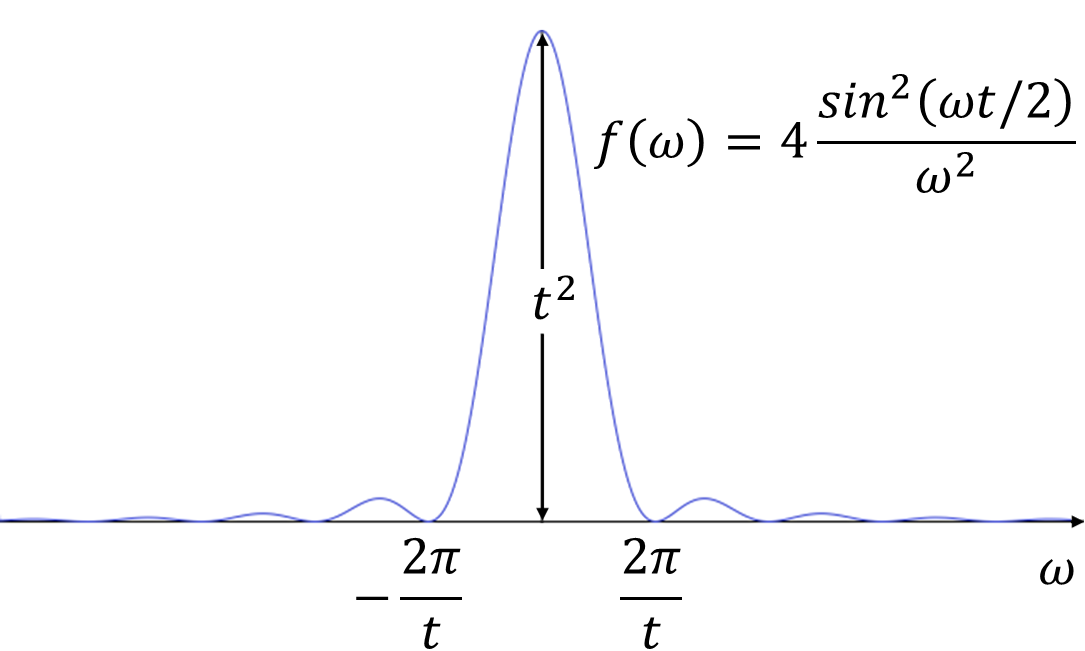
\includegraphics[width=8cm]{immagini/cap_15/fig_15_1.png}
\end{center}
\end{figure}

ossia la probabilità di transizione differisce apprezzabilmente da zero solo per quegli stati finali che soddisfano
\begin{equation}
\vert \omega \vert = \frac{\vert E_n ^{(0)} - E_i ^{(0)}\vert}{\hbar} \leq \frac{2\pi}{t}.
\end{equation}
In altri termini, se indichiamo con $\Delta t$ l'intervallo di tempo durante il quale la perturbazione ha agito sul sistema e con $\Delta E = \vert E_n ^{(0)} - E_i ^{(0)}\vert$ la differenza delle energie imperturbate relativi agli stati finale ed iniziale, si può avere con probabilità apprezzabile una transizione sole se
\begin{equation}
\Delta E \Delta t \sim \hbar .
\label{eq:cap15_7}
\end{equation}
Questa relazione è anche detta \textbf{relazione di indeterminazione tempo-energia}.\\
L'espressione (\ref{eq:cap15_6}) per la probabilità di transizione $i\rightarrow n$ e la condizione (\ref{eq:cap15_7}) che ne segue esprimono il seguente risultato: se $E_n ^{(0)}$ differisce apprezzabilmente da   $E_i ^{(0)}$, la probabilità di transizione $i \rightarrow n$ è piccola e tale rimane per tutti i valori di $t$. Questo risultato è richiesto dalla  \textbf{legge di conservazione dell'energia}. L'energia totale $E$ è costante, perché l'hamiltoniana $H$ non dipende esplicitamente dal tempo, pertanto l'energia propria $E^{(0)}$ (cioè l'energia che si ottiene trascurando la parte $V$ dovuta alla perturbazione), essendo approssimativamente uguale ad $E$, deve essere approssimativamente costante. Ciò significa che se $E^{(0)}$ ha inizialmente il valore $E _i ^{(0)}$, in qualsiasi istante successivo ci deve essere solo una probabilità piccola che esso abbia un valore considerevolmente diverso da $E _i ^{(0)}$.\\
La relazione (\ref{eq:cap15_7}) ci dice anche che un'interazione, sia pure arbitrariamente debole, che agisce per un tempo $\Delta t$, può variare l'energia propria del sistema di una quantità $\Delta E \sim \hbar /\Delta t$.\\
Questo risultato, puramente quantistico, ha un significato fisico profondo. Esso prova che \textbf{nella meccanica quantistica la legge di conservazione dell'energia può essere verificata mediante una misura soltanto a meno di una grandezza dell'ordine di} $\hbar /\Delta t$, \textbf{dove } $\Delta t$ \textbf{è la durata del processo di misura}. Infatti, una sia pur debole interazione tra lo strumento di misura ed il sistema in esame, che agisce per un tempo $\Delta t $, può sempre variare l'energia del sistema di una quantità $\Delta E \sim \hbar /\Delta t$.\\
È utile sottolineare che il \textbf{significato} della relazione (\ref{eq:cap15_7}) è \textbf{essenzialmente diverso da quello della relazione di indeterminazione} $\Delta p \Delta x\sim \hbar$, per la coordinata e la quantità di moto. In quest'ultima $\Delta p$ e $\Delta x$ sono le indeterminazioni nei valori della quantità di moto e della coordinata in uno stesso istante;  essa mostra che queste due grandezze non possono avere contemporaneamente valori esattamente determinati. L'energia $E ^{(0)}$, invece, può essere misurata in ogni istante con la precisione voluta. La grandezza $\Delta E = E_n ^{(0)} - E_i ^{(0)}$ è la differenza di sue valori esattamente misurati dell'energia $E^{(0)}$ in due stati, e non l'indeterminazione nei valori dell'energia in un istante determinato.\\
È utile mostrate che per \textbf{grandi tempi} $t$, \textbf{la probabilità di transizione} $P_{i\rightarrow n} (t) \simeq \vert c_n ^{(1)} (t) \vert ^2$ \textbf{espressa dalla relazione (\ref{eq:cap15_6}), può essere considerata proporzionale a } $t$.\\
A questo scopo osserviamo che vale la formula seguente:
\begin{equation}
\lim _{t \rightarrow \infty} \frac{\sin ^2 (\alpha t)}{\pi t \alpha ^2} = \delta (\alpha),
\label{eq:cap15_8}
\end{equation}
infatti per $\alpha \neq 0$ questo limite è nullo, mentre per  $\alpha = 0$. Si ha $\sin ^2 (\alpha t)/\alpha ^2 t = t$, cosicché il limite è infinito. Integrando poi in $d \alpha$ da $-\infty$ a $+\infty$ si ottiene (sostituendo $\alpha t = \xi$)
\begin{equation}
\frac{1}{\pi t}\int _{-\infty} ^{+\infty} d\alpha \ \frac{\sin ^2 (\alpha t)}{ \alpha ^2} = \frac{1}{\pi}\int _{-\infty} ^{+\infty} d\xi \ \frac{\sin ^2 \xi}{ \xi ^2}=1. 
\end{equation}
In tal modo la funzione a primo membro della (\ref{eq:cap15_8}) soddisfa effettivamente tutte le condizioni che definiscono una funzione $\delta$. Il risultato espresso nell'eq. (\ref{eq:cap15_8}) può essere anche visualizzato dal grafico della funzione $f(\omega)$ presentato in precedenza. Al crescere del tempo $t$ l'altezza del picco centrale della funzione cresce (proporzionalmente a $t^2$) e la sua larghezza decresce (proporzionalmente ad $1/t$). L'integrale della funzione, ossia l'area sottesa dalla curva è proporzionale a $t^2\cdot 1/t =t$, e dunque la funzione $f(\omega)/t$ ha, per grandi $t$, area costante, come richiesto dalla funzione $\delta$.\\
Conformemente a quanto detto, troviamo dall'eq. (\ref{eq:cap15_6}) che \textbf{per grandi tempi}
\begin{equation}
\vert c_n ^{(1)} (t) \vert ^2 \simeq \frac{1}{\hbar ^2} \vert V_{ni} \vert ^2 \pi t\ \delta\left(\frac{E_n ^{(0)}-E_i ^{(0)}}{2\hbar} \right),
\end{equation}
ossia, osservando che $\delta (ax) = \frac{1}{a} \delta (x)$,
\begin{equation}
\vert c_n ^{(1)} (t) \vert ^2 \simeq \frac{2\pi}{\hbar } \vert V_{ni} \vert ^2  t\ \delta (E_n ^{(0)}-E_i ^{(0)} ),
\label{eq:cap15_9}
\end{equation}
che mostra, come anticipato, che la probabilità di transizione cresce linearmente con il tempo $t$.
È consuetudine considerare la \textbf{probabilità di transizione per unità di tempo}, definita come
\begin{equation}
W_{i\rightarrow n} (t) =\frac{d}{dt} P_{i\rightarrow n} (t),
\end{equation}
che è dunque costante per grandi t.\\
Dall'eq. (\ref{eq:cap15_9}) otteniamo allora:
\begin{equation}
W_{i\rightarrow n} (t) = \frac{2\pi}{\hbar } \vert V_{ni} \vert ^2\ \delta (E_n ^{(0)}-E_i ^{(0)} ).
\label{eq:cap15_10}
\end{equation}
Questo risultato,di grande importanza pratica, è chiamato \textbf{regola d'oro di Fermi} (sebbene la teoria perturbativa dipendete dal tempo sia stata di fatto sviluppata da Dirac).		
L'eq. (\ref{eq:cap15_10}) ha particolare rilevanza per le transizioni nello spettro continuo che, praticamente, cono sempre degeneri. In questo caso le probabilità di transizione a tutti i possibili stati finali con energia $E_n ^{(0)}= E_i ^{(0)}$ si ottiene integrando l'eq. (\ref{eq:cap15_10}) con
\begin{equation}
\int dE_n ^{(0)} \ \rho (E_n ^{(0)}),
\end{equation}
dove $\rho (E)$ rappresenta la \textbf{densità degli stati}, ossia il numero di stati nell'intervallo di energia $(E, E+dE)$.
\section{Transizioni per effetto di una perturbazione periodica}
Consideriamo ora le transizioni indotte da una \textbf{perturbazione periodica}, della forma cioè
\begin{equation}
V(t) = Fe^{-i\omega t} + F^+ e ^{i\omega t},
\label{eq:cap15_11}
\end{equation}
dove $F$ è un operatore non dipendente dal tempo (funzione in generale degli operatori impulso, posizione e spin). Osserviamo che $V(t)$ è un operatore hermitiano, come deve essere.		
Assumendo ancora che al tempo $t=0$ il sistema si trovi nell'autostato $\vert i ^{(0)}\rangle$ dell'hamiltoniano imperturbato $H_0$ (per cui $c_k (0) = \delta _{ik}$ e sostituendo il potenziale (\ref{eq:cap15_11}) nella (\ref{eq:cap15_5}), si ricava:
\begin{eqnarray}
c_n ^{(1)}(t) & = & -\frac{i}{\hbar}\int _0 ^t dt'\ V_{ni} (t') \ e^{i\omega _{ni}t'} = \nonumber \\
&=& -\frac{i}{\hbar}\int _0 ^t dt'\left[ F_{ni}\ e^{i(\omega _{ni}-\omega) t'} + F_{ni} ^+\ e ^{i(\omega _{ni} +\omega) t}\right] = \nonumber \\
&=& -\frac{i}{\hbar}\left[ F_{ni}\ \frac{e^{i(\omega _{ni}-\omega) t}-1}{i(\omega _{ni}-\omega)} + F_{ni} ^+\ \frac{e ^{i(\omega _{ni} +\omega) t}-1}{i(\omega _{ni}+\omega)}\right], 
\end{eqnarray}
ossia
\begin{eqnarray}
c_n ^{(1)}(t)&=&-\frac{2i}{\hbar}\left[ F_{ni}\ e^{i\frac{(\omega _{ni}-\omega) t}{2}}\frac{\sin(\frac{(\omega _{ni}-\omega) t}{2})}{(\omega _{ni}-\omega)} +\right. \nonumber \\
& &\left. + F_{ni} ^+\ e^{i\frac{(\omega _{ni}+\omega) t}{2}}\frac{\sin(\frac{(\omega _{ni}+\omega) t}{2})}{(\omega _{ni}+\omega)}\right].
\label{eq:cap15_12}
\end{eqnarray}
Dai risultati del paragrafo precedente è evidente che, nel calcolo delle probabilità di transizione $\vert c_n ^{(1)}(t)\vert ^2$, il primo termine della (\ref{eq:cap15_12}) fornisce, per tempi grandi, un contributo significativo solo alle transizioni verso quegli stati con energia $E_n ^{(0)} \simeq E_i ^{(0)}+ \hbar \omega $, tali cioè che la differenza  $\omega _{ni} - \omega$ sia piccola. Analogamente il secondo termine della (\ref{eq:cap15_12}) fornisce un contributo significativo solo per le transizioni verso quegli stati con energia  $E_n ^{(0)} \simeq E_i ^{(0)}- \hbar \omega $, per i quali cioè la somma $\omega _{ni} + \omega$ è piccola. Infine  il termine di ``doppio prodotto'' nel calcolo di  $\vert c_n ^{(1)}(t)\vert ^2$ fornisce un contributo che è sempre trascurabile nel limite di tempi grandi, giacché le due condizioni $\omega _{ni} - \omega\simeq 0$ e $\omega _{ni} + \omega\simeq 0$ non sono mai simultaneamente verificate.\\
Dai risultati del paragrafo precedente possiamo ottenere direttamente l'espressione delle \textbf{probabilità di transizione per unità di tempo} valida nel limite di grandi $t$:
\begin{eqnarray}
W_{i\rightarrow n} &=& \frac{2\pi}{\hbar}\left[ \vert F_{ni}\vert ^2 \ \delta (E_n^{(0)}-E_i^{(0)}-\hbar \omega) + \right.\nonumber \\
& &\left. +\vert F_{ni} ^+\vert ^2 \ \delta (E_n^{(0)}-E_i^{(0)}+\hbar \omega)\right],
\label{eq:cap15_13}
\end{eqnarray}
in accordo nuovamente con la \textbf{regolo d'oro di Fermi}.\\
Il significato fisico dei due termini nell'eq. (\ref{eq:cap15_13}) è evidente. Il primo termine corrisponde alle transizioni verso quegli stati, tipicamente nello spettro del continuo, la cui energia $E_n ^{(0)}$ è accresciuta rispetto all'energia dello stato iniziale di una quantità $\hbar \omega$. Questo termine descrive dunque \textbf{l'assorbimento da parte del sistema di una quantità di energia $\hbar \omega$ dal potenziale periodico $V$}. Il secondo termine della (\ref{eq:cap15_13}) corrisponde invece alle transizioni verso quegli stati la cui energia $E_n ^{(0)}$ è minore di una quantità $\hbar \omega$ rispetto all'energia dello stato iniziale $E_i ^{(0)}$. Questo termine descrive il cosiddetto processo di \textbf{emissione stimolata, in cui il sistema cede una quantità $\hbar \omega$ della sua energia al campo esterno $V$. Così una perturbazione dipendente dal tempo può essere vista come una inesauribile sorgente o pozzo di energia}.\\
I due processi di assorbimento ed emissione stimolato posso essere schematicamente rappresentati nel modo seguente:
\begin{figure}[!htbp]
\begin{center}
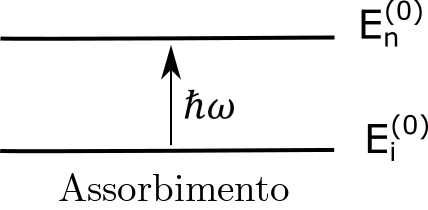
\includegraphics[width=6cm]{immagini/cap_15/fig_15_2.png}\hspace{1cm}
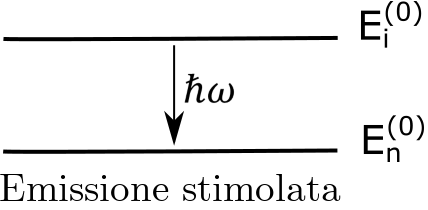
\includegraphics[width=6cm]{immagini/cap_15/fig_15_3.png}
\end{center}
\end{figure}
\newpage
\section*{Appendice al capitolo - I}
Determiniamo l'integrale
\begin{equation}
I= \int _{-\infty} ^{-\infty} dx\ \frac{\sin ^2 x}{x^2}.
\end{equation}
in primo luogo trasformiamo l'integrale con una integrazione per parti:
\begin{eqnarray}
I &=& \int _{-\infty} ^{-\infty} dx\ \frac{d}{dx}\left(\frac{1}{x}\right)\sin ^2 x = \nonumber \\
&=& \left. \frac{1}{x}\sin ^2 x\right\vert _{-\infty} ^{-\infty} +\int _{-\infty} ^{-\infty} dx\ \frac{1}{x} 2 \sin x \cos x =\\
&=& \int _{-\infty} ^{-\infty} dx\ \frac{\sin 2 x}{x}, \nonumber
\end{eqnarray}
ossia
\begin{equation}
I= \int _{-\infty} ^{-\infty} dx\ \frac{\sin  x}{x}. \quad \textrm{[Integrale di Dirichelet]}
\end{equation}
Possiamo poi trasformare l'integrale in un integrale nel piano complesso:
\begin{equation}
I= \int _{-\infty} ^{-\infty} dx\ \frac{\sin  x}{x}= \textrm{Im}\left\{\textrm{PV} \int _{-\infty} ^{-\infty} dz\ \frac{e^{iz}}{z}\right\},
\label{eq:cap15_14}
\end{equation}
dove PV indica il valor principale (la parte reale dell'integrale non è altrimenti definita per il polo in $z=0$). Per calcolare l'integrale scegliamo il seguente contorno:
\begin{figure}[!htbp]
\begin{center}
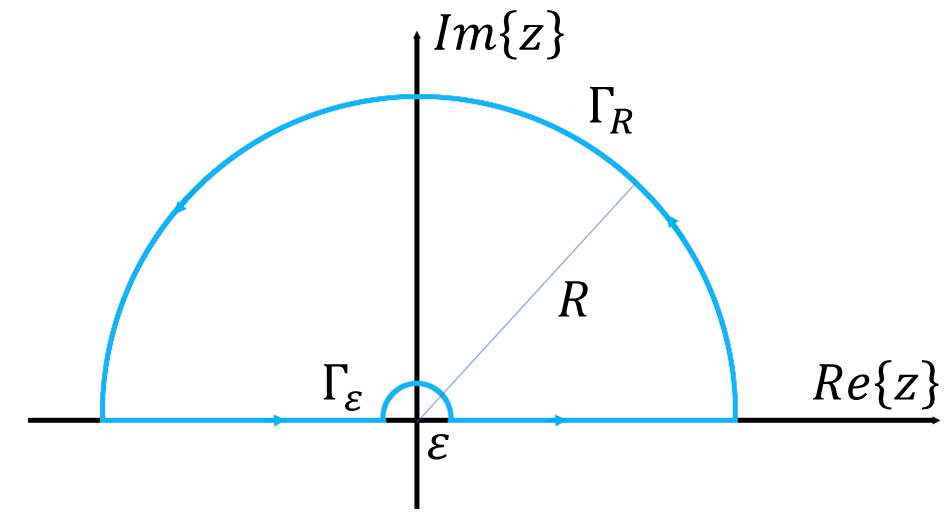
\includegraphics[width=8cm]{immagini/cap_15/fig_15_4.png}
\end{center}
\end{figure}
poiché la funzione integranda non ha poli all'interno del contorno possiamo scrivere:
\begin{eqnarray}
0 & = & \oint  dz\ \frac{e^{iz}}{z} = \nonumber \\
&=& \lim _{R\rightarrow \infty} \lim _{\varepsilon\rightarrow 0} \left[ \int _{-R} ^{-\varepsilon}dz\ \frac{e^{iz}}{z}+\int _{\varepsilon} ^{R}dz\ \frac{e^{iz}}{z}+\int _{\Gamma _{\varepsilon}} dz\ \frac{e^{iz}}{z} +\int _{\Gamma _{R}} dz\ \frac{e^{iz}}{z}\right] = \nonumber\\
&= &\textrm{PV}\int _{-\infty} ^{+\infty}dz\ \frac{e^{iz}}{z}+ \lim _{\varepsilon\rightarrow 0}  \int _{\Gamma _{\varepsilon}} dz\ \frac{e^{iz}}{z}+\lim _{R\rightarrow \infty}\int _{\Gamma _{R}} dz\ \frac{e^{iz}}{z}.
\label{eq:cap15_15}
\end{eqnarray}
L'integrale sul semicerchio esterno tende evidentemente a zero nel limite $R\rightarrow \infty $:
\begin{eqnarray}
\int _{\Gamma _{R}} dz\ \frac{e^{iz}}{z} &\overset{z= Re^{i\varphi}}{=}& \int _0 ^{\pi} d\varphi \ i R e^{i\varphi}\ \frac{e^{iRe^{i\varphi}}}{Re^{i\varphi}} = \nonumber\\
&=&i\int _0 ^{\pi} d\varphi \ e^{iRe^{i\varphi}} \underset{R\rightarrow \infty}{\longrightarrow}0.
\end{eqnarray}
L'integrale su $\Gamma _{\varepsilon}$ dà invece contributo non nullo:
\begin{eqnarray}
\int _{\Gamma _{\varepsilon}} dz\ \frac{e^{iz}}{z} &\overset{z= \varepsilon e^{i\varphi}}{=} &\int _0 ^{\pi} d\varphi \ i \varepsilon e^{i\varphi}\ \frac{e^{i\varepsilon e^{i\varphi}}}{\varepsilon e^{i\varphi}} = \nonumber\\
&=&i\int _0 ^{\pi} d\varphi \ e^{i\varepsilon e^{i\varphi}} \underset{\varepsilon\rightarrow 0}{\longrightarrow}i\int _0 ^{\pi} d\varphi = -i\pi.
\end{eqnarray}
Sostituendo questo risultato nella (\ref{eq:cap15_15}) si ottiene
\begin{equation}
\textrm{PV} \int _{-\infty} ^{-\infty} dz\ \frac{e^{iz}}{z} =-\lim _{\varepsilon \rightarrow 0} \int _{\Gamma _{\varepsilon}} dz\ \frac{e^{iz}}{z}= +i\pi.
\end{equation}
L'eq. (\ref{eq:cap15_14}) implica allora:
\begin{equation}
I= \int _{-\infty} ^{-\infty} dx\ \frac{\sin ^2  x}{x^2}= \int _{-\infty} ^{-\infty} dx\ \frac{\sin  x}{x}= \pi
\end{equation}
\newpage
\section*{Appendice al capitolo - II}
Determiniamo l'espressione per i coefficienti $c_n(t)$ al secondo ordine della teoria delle perturbazioni. L'eq. (\ref{eq:cap15_3}) comporta:
\begin{equation}
i\hbar \frac{dc_n ^{(2)} (t)}{dt} = \sum _k V_{nk} (t)\ c_k ^{(1)}(t) e^{i\omega _{nk}t},
\end{equation}
che può essere direttamente integrata, con la condizione iniziale $c_n ^{(2)} (0)=0 $, per dare:
\begin{equation}
c_n ^{(2)} (t)= -\frac{i}{\hbar}\sum _k \int _0 ^t dt'\ V_{nk} (t')\ c_k ^{(1)} (t') e ^{i\omega _{nk} t'}.
\end{equation}
Sostituendo quindi in questa espressione il risultato (\ref{eq:cap15_5}) per i coefficienti al primo ordine si ottiene dunque
\begin{equation}
c_n ^{(2)} (t)= \left(-\frac{i}{\hbar}\right)^2 \sum _{k,k'} \int _0 ^t dt'\ V_{nk} (t')\ c_k ^{(1)} (t') e ^{i\omega _{nk} t'}\int _0 ^t dt''\ V_{kk'} (t'')\  e ^{i\omega _{kk'} t''}\ c_{k'} ^{(1)} (0).
\end{equation} %DEFINITIVO
\chapter{Momento angolare}
\section[Rotazioni, momento angolare e regole di commutazione]{Rotazioni, momento angolare e regole di commutazione per gli operatori momento angolare\footnote{S3.1; LL26}}
Nella meccanica quantistica, così come nella meccanica classica, \textbf{il momento angolare è il generatore delle rotazioni infinitesime}.\\
Se indichiamo con $D_{\widehat{n}} (d\varphi)$ l'operatore unitario che induce una rotazione di un angolo infinitesimo $d\varphi$ attorno all'asse caratterizzato dal vettore $\widehat{n}$ abbiamo allora
\begin{equation}
D_{\widehat{n}} (d\varphi)=1-\frac{i}{\hbar}\vec{J}\cdot \widehat{n}\ d\varphi ,
\end{equation}
dove $\vec{J}$ è \textbf{l'operatore momento angolare}. Questa equazione può essere considerata la \textbf{definizione} nella meccanica quantistica dell'operatore momento angolare.\\
Una rotazione finita si può ottenere associando successivamente rotazioni infinitesime attorno allo stesso asse. Così ade esempio, per una rotazione finita di un angolo $\phi$ attorno all'asse $z$, otteniamo
\begin{eqnarray}
D_z (\phi) &=& \lim _{N\rightarrow \infty} \left(1-\frac{i}{\hbar} J_z \frac{\phi}{N}\right) ^N= \nonumber \\
&=& \lim _{N\rightarrow \infty} e^{N\log\left(1-\frac{i}{\hbar} J_z \frac{\phi}{N}\right)}= \lim _{N\rightarrow \infty} e^{N\left(-\frac{i}{\hbar} J_z \ \frac{\phi}{N}\right)},
\end{eqnarray}
ossia
\begin{equation}
D_z (\phi)=e^{-\frac{i}{\hbar} J_z \phi}.
\end{equation}
\textbf{L'avere assunto che il momento angolare è il generatore delle rotazioni spaziali implica che, per un sistema invariante rispetto a rotazioni attorno a un determinato asse, si conserva la componete del momento angolare lungo quell'asse.}\\
In particolare poi, le proprietà di isotropia dello spazio (ossia l'equivalenza di tutte le direzioni nello spazio) implica che l'hamiltoniano di un sistema isolato deve essere invariante rispetto a rotazioni di un angolo arbitrario attorno a un asse qualsiasi. \textbf{La legge di conservazione del momento angolare di un sistema isolato è dunque conseguenza della proprietà di isotropia dello spazio}.\\

È una proprietà ben nota delle rotazioni il fatto che \textbf{rotazioni attorno ad uno stesso asse commutano, mentre rotazioni attorno ad assi diversi non commutano}. Così ad esempio una rotazione di $\pi /2$ attorno all'asse $z$ seguita da una rotazione di $\pi /2$ attorno all'asse $x$ produce un risultato diverso di quello ottenuto con una rotazione di $\pi /2$ attorno all'asse $x$ seguita da una rotazione di $\pi /2$ attorno all'asse $z$:\\
\begin{figure}[!htbp]
\begin{center}
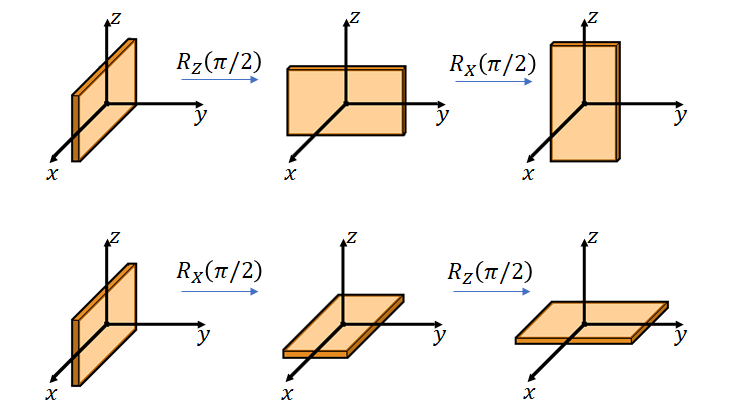
\includegraphics[width=10cm]{immagini/cap_16/fig_16_1.png}
\end{center}
\end{figure}


In termini dell'azione degli operatori di rotazione du un generico vettore di stato $\vert \alpha \rangle$ questo implica
\begin{equation}
D_x (\pi/2) D_z (\pi/2) \vert \alpha \rangle \neq D_x (\pi/2) D_x (\pi/2) \vert \alpha \rangle ,
\end{equation}
o, equivalentemente, per l'arbitrarietà dello stato $\vert \alpha \rangle$,
\begin{equation}
[D_x (\pi/2); D_z (\pi/2)] \neq 0 .
\end{equation}
Per stabilire quantitativamente le regole di commutazione degli operatori di rotazione attorno ad assi diversi, dobbiamo considerare con maggior dettaglio le proprietà di commutazione delle rotazioni.\\
A tale scopo ricordiamo che a ciascuna rotazione, diciamo di un angolo $\varphi$ attorno ad un asse definito dal versore $\widehat{n}$, può essere associata una \textbf{matrice ortogonale} $R_{\widehat{n}} (\varphi)$. Il significato di questa matrice è che un vettore $\vec{v}$ di componenti $(v_x, v_y v_z) $ ( che può rappresentare ad esempio la posizione di una particella nello spazio), viene trasformato, a seguito della rotazione nel vettore $\vec{v'}$ legato a $\vec{v}$ dalla relazione
\begin{equation}
\vec{v'}= R_{\widehat{n}} (\varphi)\vec{v}.
\end{equation}
L'ortogonalità della matrice $R$ segue dal fatto che le rotazioni lasciano invariati i moduli dei vettori:
\begin{equation}
\vec{v'}\cdot\vec{v} = \vec{v}R^T R \vec{v}= \vec{v}\cdot\vec{v} \qquad \Rightarrow \quad
 R^T R =1.
\end{equation}
È semplice derivare l'espressione della matrice di rotazione associata ad esempio ad una rotazione di un angolo $d\varphi $ attorno all'asse $z$. Esprimendo le componenti del vettore $\vec{v}$ in coordinate polari,
\begin{equation}
\begin{cases}
v_x = v \sin\theta \cos \varphi ,\\
v_y = v \sin\theta \sin \varphi ,\\
v_z = v \cos\theta ,
\end{cases}
\end{equation}
si ha che il vettore $\vec{v}$ si trasforma, per effetto della rotazione, nel vettore $\vec{v'}$ di componenti:
\begin{equation}
\begin{cases}
v'_x = v \sin\theta \cos (\varphi +d\varphi )= v_x \cos d\varphi - v_y \sin d\varphi ,\\
v'_y = v \sin\theta \sin (\varphi +d\varphi ) = v_x \sin d\varphi + v_y \cos d\varphi ,\\
v'_z = v \cos\theta = v_z .
\end{cases}
\end{equation}
La matrice $R_z (d\varphi)$ ha dunque la forma
\begin{equation}
R_z (d\varphi)=
\begin{pmatrix}
\cos d\varphi & -\sin d\varphi & 0\\
\sin d\varphi & \cos d\varphi & 0 \\
0 & 0 & 1 \\
\end{pmatrix}
\end{equation}
Per studiare le proprietà di commutazione delle rotazioni è conveniente considerare rotazioni infinitesime. Ponendo $\varepsilon =d\varphi$ e sviluppando la precedente matrice fino al secondo ordine in $\varepsilon$ troviamo:
\begin{equation}
R_z (\varepsilon)=
\begin{pmatrix}
1-\varepsilon ^2 /2 & -\varepsilon & 0\\
\varepsilon & 1-\varepsilon ^2/2 & 0 \\
0 & 0 & 1 \\
\end{pmatrix}
+ O(\varepsilon ^3).
\end{equation}
Le corrispondenti matrici si rotazione attorno agli assi $x$ e $y$ si possono ottenere con permutazioni cicliche di $x$, $y$ e $z$:
\begin{equation}
x\rightarrow y,\ y\rightarrow z,\ z\rightarrow x,
\end{equation}
si ottiene in tal modo:
\begin{equation}
R_x (\varepsilon)=
\begin{pmatrix}
1 & 0 & 0\\
0 & 1-\varepsilon ^2/2 & -\varepsilon \\
0 & \varepsilon & 1-\varepsilon ^2/2 \\
\end{pmatrix}
+ O(\varepsilon ^3),
\end{equation}
\begin{equation}
R_y (\varepsilon)=
\begin{pmatrix}
1-\varepsilon ^2/2 & 0 & \varepsilon\\
0 & 1 &0 \\
- \varepsilon & 0 & 1-\varepsilon ^2/2 \\
\end{pmatrix}
+ O(\varepsilon ^3).
\end{equation}
Consideriamo ora una rotazione di angolo $\varepsilon$ attorno all'asse $y$ seguita da una rotazione di angolo $\varepsilon$ attorno all'asse $x$. La corrispondente matrice di rotazione è:
\begin{equation}
R_x (\varepsilon)R_y (\varepsilon)=
\begin{pmatrix}
1-\varepsilon ^2/2 & 0 & \varepsilon \\
 \varepsilon ^2 & 1-\varepsilon ^2/2 & -\varepsilon \\
-  \varepsilon & \varepsilon & 1-\varepsilon ^2 \\
\end{pmatrix}
+ O(\varepsilon ^3)
\end{equation}
Se consideriamo invece rotazione di angolo $\varepsilon$ attorno all'asse $x$ seguita da una rotazione di angolo $\varepsilon$ attorno all'asse $y$ otteniamo la matrice di rotazione
\begin{equation}
R_y (\varepsilon)R_x (\varepsilon)=
\begin{pmatrix}
1-\varepsilon ^2/2 & \varepsilon ^2 & \varepsilon \\
 0 & 1-\varepsilon ^2/2 & -\varepsilon \\
-  \varepsilon & \varepsilon & 1-\varepsilon ^2 \\
\end{pmatrix}
+ O(\varepsilon ^3)
\end{equation}
NB $\displaystyle{\left[\left( R_y R_x\right) ^T = R_x ^T R_y ^T=R_xR_y+(\varepsilon\rightarrow -\varepsilon)\right]}$.\\
Dal confronto di questi risultati vediamo che
\begin{equation}
R_x (\varepsilon)R_y (\varepsilon)-R_y (\varepsilon)R_x (\varepsilon)=
\begin{pmatrix}
0 & - \varepsilon ^2 & 0 \\
 \varepsilon ^2 & 0 & 0 \\
0 & 0& 0\\
\end{pmatrix}
= R_z(\varepsilon ^2)-1+ O(\varepsilon ^3),
\end{equation}
che definisce la proprietà di commutazione di due rotazioni successive infinitesime attorno agli assi $x$ ed $y$.\\
La stessa proprietà deve essere soddisfatta dagli operatori che inducono le corrispondenti rotazioni dei vettori di stato in meccanica quantistica, ossia:
\begin{equation}
D_x (\varepsilon)D_y (\varepsilon)-D_y (\varepsilon)D_x (\varepsilon)=D_z(\varepsilon ^2)-1+ O(\varepsilon ^3).
\end{equation}
In termini degli operatori momento angolare, questa relazione implica:
\begin{eqnarray}
& &D_x (\varepsilon)D_y (\varepsilon)-D_y (\varepsilon)D_x (\varepsilon)= \nonumber\\
& & = \left(1-\frac{i\varepsilon}{\hbar} J_x -\frac{\varepsilon ^2}{2\hbar ^2}J_x ^2\right)\left(1-\frac{i\varepsilon}{\hbar} J_y -\frac{\varepsilon ^2}{2\hbar ^2}J_y ^2\right)- \left( x \leftrightarrow y\right) =\nonumber \\
& &= \left(1-\frac{i\varepsilon}{\hbar} J_x-\frac{i\varepsilon}{\hbar} J_y-\frac{\varepsilon ^2}{2\hbar ^2}J_x-\frac{\varepsilon ^2}{2\hbar ^2}J_y-\frac{\varepsilon ^2}{\hbar ^2}J_xJ_y \right) - \left( x \leftrightarrow y\right) = \nonumber \\
& & = -\frac{\varepsilon ^2}{\hbar ^2}\left(J_xJ_y-J_y J_x\right)= \nonumber \\
& & = D_z (\varepsilon ^2)- = \left(1-\frac{i\varepsilon ^2}{\hbar} J_z-\right)=-\frac{i\varepsilon ^2}{\hbar} J_z, 
\end{eqnarray}
ossia
\begin{equation}
[ J_x, J_y ] = i\hbar J_z.
\end{equation}
Utilizzando le permutazioni cicliche di $x$, $y$ e $z$ possiamo derivare le regole di commutazione per le altre componenti del momento angolare:
\begin{equation}
[ J_y, J_z ] = i\hbar J_x,
\end{equation}
\begin{equation}
[ J_z, J_x ] = i\hbar J_y,
\end{equation}
o in forma compatta per due componenti arbitrarie
\begin{equation}
[ J_i, J_j ] = i\hbar \varepsilon _{ikj}J_k.
\label{eq:cap16_1}
\end{equation}
Queste equazioni sono note come le \textbf{relazioni fondamentali di commutazione del momento angolare}.\\
Sottolineiamo come \textbf{queste relazioni di commutazione seguono solamente dall'assunzione che $J_k$ è il generatore della rotazione attorno all'asse k-esimo e dalla proprietà di non commutatività delle rotazioni}.\\
\textbf{Le relazioni di commutazione (\ref{eq:cap16_1}) implicano che, in generale, le tre componenti del momento angolare non possono avere simultaneamente valori determinati}. A questo proposito il momento angolare differisce essenzialmente dall'impulso, le cui tre componenti sono misurabili simultaneamente.		
Con gli operatori $J_x$, $J_y$ e $J_z$ formiamo l'\textbf{operatore} del \textbf{quadrato del momento angolare}:
\begin{equation}
J^2 = J_x ^2 + J_y ^2 + J_z ^2.
\end{equation}
Questo operatore commuta con ciascuno degli operatori $J_x$, $J_y$ e $J_z$:
\begin{equation}
[J^2, J_k]=0. \quad (k=1,2,3)
\label{eq:cap16_2}
\end{equation}
Infatti, considerando ad esempio il caso $k=3$ ed utilizzando le relazioni di commutazione (\ref{eq:cap16_1}) otteniamo:
\begin{eqnarray}
[J^2, J_z] &=& [J_x ^2+J_y^2+J_z ^2, J_z] = [J_x ^2, J_z]+[J_y ^2, J_z]= \nonumber \\
& =& J_x[J_x, J_z]+[J_x, J_z]J_x+J_y[J_y, J_z]+[J_y, J_z]J_y =  \nonumber \\
& = & J_x (-i\hbar J_y)+ (-i\hbar J_y)J_x+ J_y (i\hbar J_x)+(i\hbar J_x)J_y = \nonumber \\
& = & 0.  
\end{eqnarray}
(N.B.: abbiamo usato la proprietà generale dei commutatori\\ $\displaystyle{[AB,C]=A[B,C]+[A,C]B}$).\\
Dal punto di vista fisico, le relazioni (\ref{eq:cap16_2}) significano che \textbf{il quadrato del momento angolare (cioè il suo valore assoluto) può avere valori determinati contemporaneamente con una delle sue componenti}.
\section[Autovalori ed elementi di matrice degli operatori di momento angolare]{Autovalori ed elementi di matrice degli operatori di momento angolare\footnote{S3.5, LL27}}
Consideriamo il problema di determinare gli autovalori e gli autovettori simultanei del quadrato del momento angolare $J^2$ e di una sua componente lungo un determinato asse, diciamo $J_z$. Indichiamo rispettivamente con $a$ e $b$ questi autovalori.\\
Cerchiamo cioè le soluzioni delle equazioni
\begin{eqnarray}
& &J^2 \vert a, b \rangle = a \vert a, b \rangle , \\
& &J_z \vert a, b \rangle = b \vert a, b \rangle .
\end{eqnarray}
A tale scopo risulta conveniente, in luogo degli operatori $J_x$ e $J_y$, introdurre le loro combinazioni complesse
\begin{equation}
J_{\pm} = J_x \pm i J_y .
\end{equation}
Utilizzando le relazioni di commutazione (\ref{eq:cap16_1}) per le componenti del momento angolare possiamo calcolare
\begin{eqnarray}
[J_z , J_{\pm}] & = & [J_z , J_x \pm i J_y] = [J_z , J_x] \pm i [J_z ,J_y] = \nonumber \\
& = & i\hbar J_y \pm i (-i\hbar J_x) = \pm \hbar (J_x \pm i J_y ) = \pm \hbar J_{\pm} .
\end{eqnarray}
Dunque
\begin{equation}
[J_z , J_{\pm}] = \pm \hbar J_{\pm} .
\label{eq:cap16_3}
\end{equation}
Dalle relazioni di commutazione (\ref{eq:cap16_2}) segue anche immediatamente
\begin{equation}
[J^2 , J_{\pm}]=0 .
\label{eq:cap16_4}
\end{equation}
Per determinare il significato fisico degli operatori $J_{\pm}$ esaminiamo l'azione di $J_z$ sugli stati $J_{\pm} \vert a, b \rangle$:
\begin{eqnarray}
J_zJ_{\pm} \vert a, b \rangle & =& \left( [J_z,J_{\pm}] + J_{\pm}J_{z}\right)\vert a, b \rangle = \nonumber \\
&=& (b \pm \hbar )J_{\pm} \vert a, b \rangle , 
\end{eqnarray}
dove abbiamo fatto uso delle relazioni (\ref{eq:cap16_3}). Ciò prova che \textbf{gli stati $ J_{\pm} \vert a, b \rangle$ sono ancora (a meno di una costante di normalizzazione) autostati dell'operatore $J_z$ corrispondenti agli autovalori $b\pm \hbar$}. Per questa ragione gli operatori $J_{\pm}$ sono anche noti con il nome di \textbf{operatori ``a scala''}.\\
Applichiamo ora agli stati $ J_{\pm} \vert a, b \rangle$ l'operatore $J^2$. Utilizzando le regole di commutazione (\ref{eq:cap16_4}) troviamo:
\begin{equation}
J^2J_{\pm} \vert a, b \rangle = \left( [J^2,J_{\pm}] + J_{\pm}J^2\right)\vert a, b \rangle = a J_{\pm} \vert a, b \rangle .
\end{equation}
In altri termini, gli stati $J_{\pm} \vert a, b \rangle$ sono ancora autostati dell'operatore $J^2$ corrispondenti allo stesso autovalore $a$.\\
In conclusione possiamo scrivere:
\begin{equation}
J_{\pm} \vert a, b \rangle = c_{\pm}\vert a, b\pm \hbar \rangle,
\label{eq:cap16_5}
\end{equation}.
dove le costanti $c_{\pm}$ sono determinate imponendo la corretta normalizzazione dei vettori di stato.\\
Supponiamo ora di applicare più volte, in successione, l'operatore $J_+$ ad un autostato $\vert a,b \rangle $. Ad ogni applicazione l'autovalore di $J_z$ aumenta di $\hbar$, mentre l'autovalore di $J^2$ è invariato. Questo processo, tuttavia, non può continuare in modo indefinito giacché, per un fissato valore $a$ di $J^2$, deve esistere un valore massimo, $b_{MAX}$ per $J_z$. Questo segue dal fatto che la differenza $J^2-J_z ^2=J_x ^2+J_y ^2$ è l'operatore di una grandezza fisica essenzialmente positiva e i suoi autovalori non possono essere negativi:
\begin{eqnarray}
& &\langle a,b \vert J^2-J_z ^2 \vert a, b \rangle = (a-b^2) = \nonumber \\
& &=\langle a,b \vert J_x ^2+J_y ^2 \vert a, b \rangle = \nonumber \\
& & =\left(\langle a,b \vert J_x ^+\right) \left(J_x \vert a, b \rangle\right)+\left(\langle a,b \vert J_y ^+\right) \left(J_y \vert a, b \rangle\right) \geq 0.
\end{eqnarray}
Dunque
\begin{equation}
b^2 \leq a .
\label{eq:cap16_6}
\end{equation}
Deve allora esistere un $b_{MAX}$ tale che:
\begin{equation}
J_{+} \vert a, b_{MAX} \rangle =0.
\end{equation}
Per calcolare il valore di $b_{MAX}$ possiamo applicare l'operatore $J_-$ alla precedente equazione ed osservare che 
\begin{equation}
J_-J_+ = (J_x-iJ_y)(J_x+iJ_y)= J_x^2 +J_y ^2+i[J_x, J_y] ,
\end{equation}
ossia 
\begin{equation}
J_-J_+ = J^2 -J_z ^2 -\hbar J_z .
\label{eq:cap16_7}
\end{equation}
Si ha allora:
\begin{eqnarray}
0&=&J_{-}J_{+} \vert a, b_{MAX} \rangle = (J^2 -J_z ^2 -\hbar J_z)\vert a, b_{MAX} \rangle = \nonumber \\
&=&(a- b_{MAX} ^2 - \hbar b_{MAX} )\vert a, b_{MAX} \rangle,
\end{eqnarray}
ossia
\begin{equation}
b_{MAX}(b_{MAX}+\hbar) =a .
\label{eq:cap16_8}
\end{equation}
Similmente, l'eq. (\ref{eq:cap16_6}) implica anche l'esistenza di un valore minimo di $b$,  $b_{MIN}$, definito dall'equazione
\begin{equation}
J_{-} \vert a, b_{MIN} \rangle =0.
\end{equation}
Tale valore si può calcolare applicando l'operatore $J_+$ alla precedente equazione ed osservando che
\begin{equation}
J_+J_- = (J_x+iJ_y)(J_x-iJ_y)= J_x^2 +J_y ^2-i[J_x, J_y] ,
\end{equation}
ossia
\begin{equation}
J_-J_+ = J^2 -J_z ^2 +\hbar J_z .
\label{eq:cap16_9}
\end{equation}
Si trova allora
\begin{eqnarray}
0&=&J_{+}J_{-} \vert a, b_{MIN} \rangle = (J^2 -J_z ^2 +\hbar J_z)\vert a, b_{MIN} \rangle = \nonumber \\
&=&(a- b_{MIN} ^2 - \hbar b_{MIN} )\vert a, b_{MIN} \rangle ,
\end{eqnarray}
da cui
\begin{equation}
b_{MIN}(b_{MIN}-\hbar) =a .
\label{eq:cap16_10}
\end{equation}
Dal confronto delle eq. (\ref{eq:cap16_8}) e (\ref{eq:cap16_10}) (con l'ipotesi $b_{MAX} > b_{MIN}$) vediamo che
\begin{equation}
b_{MAX} = - b_{MIN} ,
\end{equation}
e dunque i valori possibili per $b$ sono compresi nell'intervallo
\begin{equation}
-b_{MAX} \leq b \leq b_{MAX} .
\end{equation}
Osserviamo che l'autostato corrispondente all'autovalore massimo di $J_z$, $\vert a, b_{MAX}\rangle$, può essere ottenuto applicando un numero $n$ (intero) di volte l'operatore $J_+$ all'autostato corrispondente all'autovalore minimo, $\vert a, - b_{MAX}\rangle $. Questo implica
\begin{equation}
b_{MAX}=-b_{MAX}+n\hbar, 
\end{equation}
cioè
\begin{equation}
b_{MAX}=\frac{n\hbar}{2}, \qquad n intero.
\end{equation}
Solitamente il valore di $b_{MAX}$ in unità $\hbar$ è indicato con $j$, così che
\begin{equation}
j= \frac{b_{MAX}}{\hbar} \frac{n}{2}, \qquad n intero.
\end{equation}
L'eq. (\ref{eq:cap16_8}) indica poi che
\begin{equation}
a= \hbar ^2 j(j+1).
\end{equation}
Definiamo anche $m$ come il generico autovalore di $J_z$ in unità $\hbar$:
\begin{equation}
b=m\hbar .
\end{equation}
Il numero $m$ può assumere allora tutti i valori compresi tra $-j$ e $j$ e distanziati tra loro di 1.\\
Possiamo quindi riassumete i \textbf{risultati} derivati per gli autovalori di $J^2$ e $J_z$ nella forma seguente:
\begin{eqnarray}
& &J^2\vert j, m \rangle =\hbar ^2 j (j+1)\vert j, m \rangle , \\
& &J_z\vert j, m \rangle =\hbar  m\vert j, m \rangle ,
\end{eqnarray}
\textbf{dove $j$ può assumere tutti i valori, interi o seminteri positivi, incluso  lo zero, ed $m$ può assumere i valori}:
\begin{equation}
m=-j, -j+1,\dots , j-1, j.
\end{equation}
È importante osservare come \textbf{la quantizzazione del momento angolare è una diretta conseguenza della sole regole di commutazione del momento  angolare che a loro volta discendono dalle proprietà delle rotazioni e della definizione di $\vec{j}$ come generatore delle rotazioni}.\\
Per concludere questo studio \textbf{deduciamo le espressioni per gli elementi di matrice delle componenti $J_x$ e $J_y$ del momento angolare nella base degli autostati di $J^2$ e $J_z$}.\\
È conveniente a tale proposito considerare dapprima gli elementi di matrice degli operatori a scala $J_+$ e $J_-$. Scriviamo allora le equazioni (\ref{eq:cap16_5}) nella forma:
\begin{equation}
\begin{cases}
J_+\vert j, m \rangle = c_{jm} ^+\vert j, m+1 \rangle , \\
J_-\vert j, m \rangle = c_{jm} ^-\vert j, m-1 \rangle ,
\end{cases}
\end{equation}
Utilizzando le equazioni (\ref{eq:cap16_7}) e (\ref{eq:cap16_9})otteniamo:
\begin{eqnarray}
\vert c_{jm} ^+\vert ^2 &=& \langle j, m \vert J_- J_+\vert j, m \rangle = \langle j, m \vert J^2- J_z ^2 -\hbar J_z\vert j, m \rangle =\nonumber \\
&=& \hbar ^2 \left( j(j+1) - m (m+1)\right) ,
\end{eqnarray}
e
\begin{eqnarray}
\vert c_{jm} ^-\vert ^2 &=& \langle j, m \vert J_+ J_-\vert j, m \rangle = \langle j, m \vert J^2- J_z ^2 +\hbar J_z\vert j, m \rangle =\nonumber \\
&=& \hbar ^2 \left( j(j+1) - m (m-1)\right) .
\end{eqnarray}
Le precedenti equazioni determinano i coefficienti $c^+$ e $c^-$ a meno di un fattore di fase. In generale si usa scegliere $c^+$ e $c^-$ reali e positivi, definendo in tal modo la fase (arbitraria) degli autostati $\vert j,m \rangle$ di $J^2$ e $J_z$. Si trova quindi:
\begin{eqnarray}
& &J_+\vert j, m \rangle =\hbar \sqrt{j(j+1)-m(m+1)}\vert j, m+1 \rangle ,  \label{eq:cap16_11} \\
& &J_-\vert j, m \rangle =\hbar \sqrt{j(j+1)-m(m-1)}\vert j, m-1 \rangle  .\label{eq:cap16_12}
\end{eqnarray}
Poiché le componenti $J_x$ e $J_y$ del momento angolare sono legate agli operatori a scala dalle semplici relazioni:
\begin{equation}
J_x= \frac{1}{2}\left(J_+ + J_-\right),\qquad J_y= \frac{1}{2i}\left(J_+ - J_-\right)
\end{equation}
le equazioni (\ref{eq:cap16_11}) e (\ref{eq:cap16_12}) ci consentono di ricavare immediatamente le espressioni cercate per gli elementi di matrice di $J_x$ e $J_y$:
\begin{eqnarray}
\langle j, m-1\vert J_x\vert j, m \rangle &=&\langle j, \vert J_x\vert j, m-1 \rangle = \nonumber \\
&=& \frac{\hbar}{2}\sqrt{j(j+1)-m(m-1)} , 
\end{eqnarray}
\begin{eqnarray}
\langle j, m-1\vert J_y\vert j, m \rangle &=& -\langle j, \vert J_y\vert j, m-1 \rangle = \nonumber \\
&=& \frac{i\hbar}{2}\sqrt{j(j+1)-m(m-1)} , 
\end{eqnarray}
tutti gli altri elementi di matrice sono invece nulli.\\
Osserviamo in particolare che nelle matrici $J_x$ e $J_y$ gli elementi diagonali sono tutti nulli. Poiché l'elemento di matrice diagonale dà il valore medio delle grandezze nello stato corrispondente, ciò significa che \textbf{negli stati con valori determinati di $J_z$, i valori medi di $J_x$ e $J_y$ sono nulli}:
\begin{equation}
\langle J_x \rangle = \langle J_y \rangle =0.
\end{equation} %DEFINITIVO
\chapter[Momento angolare orbitale]{Momento angolare orbitale\footnote{S3.6, LL26, G11}}
Abbiamo introdotto il momento angolare definendolo come il generatore delle rotazioni infinitesime. Ma quando il momento di spin è nullo (o comunque può essere ignorato) il momento angolare per una particella coincide con il \textbf{momento angolare orbitale}, definito da:
\begin{equation}
\vec{L}=\vec{r}\wedge\vec{p}
\end{equation}
Per il momento angolare orbitale, le \textbf{regole di commutazione} fondamentali,
\begin{equation}
[L_i, L_j]= i \varepsilon _{ijk}L_k ,
\label{eq:cap17_1}
\end{equation}
seguono direttamente dalle regole di commutazione degli operatori di posizione ed impulso. Si ha, ad esempio,
\begin{eqnarray}
[L_x , L_y] &=& [y p_z - zp_y, zp_x -xp_z] = \nonumber \\
&=&[y p_z , zp_x] + [zp_y, xp_z] = \nonumber \\
&=& yp_x [p_z , z] + p_y x [z , p_z] = \nonumber  \\
&=& -i\hbar (yp_x -xp_y) = i\hbar L_z ,
\end{eqnarray}
e analoghe per le altre componenti.\\
Possiamo mostrare esplicitamente come l'operatore momento angolare, definito dall'eq. (\ref{eq:cap17_1}), coincida, per particelle di spin nullo, con il \textbf{generatore delle rotazioni infinitesime}.\\
Applichiamo infatti l'operatore:
\begin{equation}
\left(1- \frac{i}{\hbar}\delta \varphi L_z\right)
\end{equation}
su un autostato arbitrario della posizione, e mostriamo come lo stato risultante sia ancora un autostato della posizione ma ruotato, rispetto allo stato di partenza, di un angolo $\delta \varphi$ attorno all'asse $z$. Questo risultato segue dalla considerazione che l'impulso è il generatore delle traslazioni infinitesime. Si ha infatti:
\begin{eqnarray}
\left(1- \frac{i}{\hbar}\delta \varphi L_z\right)\vert x', y', z'\rangle &=& \underbrace{\left[1- \frac{i}{\hbar}\delta \varphi\left(x'p_y-y'p_x\right)\right]}_{\begin{array}{cc}
\scriptstyle{(1- \frac{i}{\hbar}\vec{p}\cdot d\vec{x})}\\
\scriptstyle{d\vec{x}= (-y\delta \varphi ,\ x \delta \varphi ,\ 0)}
\end{array}}\vert x', y', z'\rangle = \nonumber \\
&=&\vert x'-y'\delta \varphi , y'+x'\delta \varphi , z'\rangle ,
\end{eqnarray}
che è quello che volevamo dimostrare.
\begin{equation}
\textrm{N.B.} \quad 
R_z (\delta \varphi)=
\begin{pmatrix}
1 & -\delta \varphi & 0\\
\delta \varphi & 1 & 0 \\
0 & 0 & 1 \\
\end{pmatrix}
\end{equation}
Lo stesso risultato può essere convenientemente espresso utilizzando, per definire l'autostato della posizione, un sistema di coordinate polari:
\begin{equation}
\left(1- \frac{i}{\hbar}\delta \varphi L_z\right)\vert r, \theta, \varphi\rangle = \vert r, \theta, \varphi + \delta\varphi\rangle .
\label{eq:cap17_2}
\end{equation}
Proponiamoci ora di derivare l'\textbf{espressione dell'operatore $L_z$ nella rappresentazione delle coordinate}.\\
Utilizzando sempre un sistema di coordinate polari, e tenendo conto dell'eq. (\ref{eq:cap17_2}), troviamo:
\begin{eqnarray}
\langle r, \theta, \varphi \vert \left(1- \frac{i}{\hbar}\delta \varphi L_z\right) \vert \alpha\rangle &=& \langle r, \theta, \varphi \vert \left(1+ \frac{i}{\hbar}\delta \varphi L_z\right) ^+ \vert \alpha\rangle =\nonumber \\
&=& \langle r, \theta, \varphi - \delta \varphi \vert\alpha\rangle  = \nonumber \\
&=& \langle r, \theta, \varphi \vert \alpha\rangle - \delta \varphi \frac{\partial}{\partial \varphi}\langle r, \theta, \varphi \vert\alpha\rangle .
\end{eqnarray}
per l'arbitrarietà dello stato $\vert \alpha \rangle$, questo risultato implica:
\begin{equation}
\langle r, \theta, \varphi \vert  L_z \vert \alpha\rangle =- i\hbar\ \frac{\partial}{\partial \varphi}\langle r, \theta, \varphi \vert\alpha\rangle ,
\end{equation}
ossia nella rappresentazione delle coordinate
\begin{equation}
L_z = -i\hbar \frac{\partial}{\partial \varphi}.
\label{eq:cap17_4}
\end{equation}
Allo stesso stato si può giungere, altrettanto facilmente, utilizzando l'espressione nella rappresentazione delle coordinate  dell'operatore impulso. Si ha infatti:
\begin{equation}
L_z= xp_y-yp_x = -i\hbar \left( x\frac{\partial}{\partial y} -y\frac{\partial}{\partial x}\right) .
\label{eq:cap17_3}
\end{equation}
Esprimiamo questo risultato utilizzando un sistema di coordinate polari. Dalle relazioni
\begin{equation}
\begin{cases}
x=r\sin \theta \cos \varphi \\
y=r\sin \theta \sin \varphi \\
z= r\cos\theta
\end{cases}
\qquad
\begin{cases}
r=(x^2+y^2+z^2)^{1/2} \\
\theta=\arctan\left(\sqrt{(x^2+y^2)/z^2}\right) \\
\varphi= \arctan \left(y/x\right)
\end{cases}
\end{equation}
si derivano, con una semplice algebra, le relazioni\footnote{$\partial/\partial x \arctan x = 1/(1+x^2)$}
\begin{equation}
\begin{cases}
\displaystyle{\frac{\partial}{\partial x} = \frac{\partial r}{\partial x}\frac{\partial}{\partial r}+\frac{\partial \theta}{\partial x}\frac{\partial}{\partial \theta}+ \frac{\partial \varphi}{\partial x}\frac{\partial}{\partial \varphi} = }\\
\qquad = \displaystyle{\sin\theta \cos \varphi \frac{\partial}{\partial r}+\cos\theta \cos \varphi\frac{1}{r} \frac{\partial}{\partial \theta}-\frac{\sin \varphi}{r\ \sin \theta} \frac{\partial}{\partial \varphi}}; \\
\\
\displaystyle{\frac{\partial}{\partial y} = \frac{\partial r}{\partial y}\frac{\partial}{\partial r}+\frac{\partial \theta}{\partial y}\frac{\partial}{\partial \theta}+ \frac{\partial \varphi}{\partial y}\frac{\partial}{\partial \varphi} = }\\
\qquad = \displaystyle{\sin\theta \sin \varphi \frac{\partial}{\partial r}+\cos\theta \sin \varphi\frac{1}{r} \frac{\partial}{\partial \theta}+\frac{\cos \varphi}{r\ \sin \theta} \frac{\partial}{\partial \varphi}}; \\
\\
\displaystyle{\frac{\partial}{\partial z} = \frac{\partial r}{\partial z}\frac{\partial}{\partial r}+\frac{\partial \theta}{\partial z}\frac{\partial}{\partial \theta}+ \frac{\partial \varphi}{\partial z}\frac{\partial}{\partial \varphi} = }\\
\qquad = \displaystyle{\cos\theta\frac{\partial}{\partial r}-\frac{\sin \theta}{r} \frac{\partial}{\partial \theta}}.
\end{cases}
\end{equation}
Dall'espressione (\ref{eq:cap17_3}) dell'operatore $L_z$ si ottiene pertanto
\begin{eqnarray}
L_z &=&-i\hbar \left[ r\sin \theta \cos \varphi \left(\sin \theta \sin \varphi \frac{\partial}{\partial r}+\cos \theta \sin \varphi\frac{1}{r} \frac{\partial}{\partial \theta}+ \right.\right. \nonumber \\
& &\left. + \frac{\cos \varphi}{r\ \sin \theta} \frac{\partial}{\partial \varphi}\right) - r \sin \theta \sin \varphi \left( \sin \theta \cos \varphi \frac{\partial}{\partial r}+\right. \nonumber \\
& & \left. \left. \cos \theta \cos \varphi\frac{1}{r} \frac{\partial}{\partial \theta}-\frac{\sin \varphi}{r\ \sin \theta} \frac{\partial}{\partial \varphi}\right)\right] ,
\end{eqnarray}
ossia
\begin{equation}
L_z = -i\hbar \frac{\partial}{\partial \varphi},
\end{equation}
in accordo con quanto ricavato precedentemente.\\
In modo analogo si possono derivare le \textbf{espressioni degli operatori nella rappresentazione delle coordinate}. Risulta conveniente, a tale scopo, derivare prima queste espressioni per gli operatori $L_{\pm}$:
\begin{eqnarray}
L_{\pm} &=& L_x \pm iL_y = (yp_z-zp_y) \pm i(zp_x-xp_z)= \nonumber \\
&=& \mp i (x\pm iy)p_z \pm iz(p_x\pm ip_y)= \nonumber \\
&=&\mp \hbar \left[ \left(x\pm i y\right) \frac{\partial}{\partial z}- z \left( \frac{\partial}{\partial x}\pm i\frac{\partial}{\partial y}\right) \right] ,
\end{eqnarray}
da cui, sostituendo le coordinate polari:
\begin{eqnarray}
L_{\pm} &=&\mp \hbar \left[ r\sin \theta\ e^{\pm i \varphi}\ \left( \cos \theta\frac{\partial}{\partial r} -\frac{\sin \theta}{r}\frac{\partial}{\partial \theta} \right)- \right. \nonumber \\
& &\left. - r\cos \theta \left( \sin \theta\ e^{\pm i \varphi}\frac{\partial}{\partial r}+\frac{\cos \theta}{r} e^{\pm i \varphi}\frac{\partial}{\partial \theta}\pm\frac{i e^{\pm i \varphi}}{r\sin \theta}\frac{\partial}{\partial \varphi} \right)\right]= \nonumber \\
&=& \mp \hbar e^{\pm i \varphi}\left(-\frac{\partial}{\partial \theta}\mp i\ \cot \theta\frac{\partial}{\partial \varphi}\right) ,
\end{eqnarray}
ossia, infine
\begin{equation}
L_{\pm}=\hbar e^{\pm i \varphi}\left[\pm \frac{\partial}{\partial \theta}+ i\ \cot \theta\frac{\partial}{\partial \varphi}\right] .
\label{eq:cap17_5}
\end{equation}
Da questo risultato è poi immediato ricavare le espressioni degli operatori $L_x$ ed $L_y$ nella rappresentazione delle coordinate. Ricordando le relazioni:
\begin{equation}
L_x = \frac{1}{2} (L_+ + L_-) \qquad L_y = \frac{1}{2i} (L_+ + L_-),
\end{equation}
si ottiene
\begin{eqnarray}
& &L_x =i\hbar \left( \sin \varphi \frac{\partial}{\partial \theta}+\cot \theta \cos \varphi \frac{\partial}{\partial \varphi}\right)\\
& &L_y =i\hbar \left(- \cos \varphi \frac{\partial}{\partial \theta}+\cot \theta \sin \varphi \frac{\partial}{\partial \varphi}\right) .
\end{eqnarray}
Risulta infine utile determinare l'\textbf{espressione, nella rappresentazione delle coordinate, del quadrato del momento angolare orbitale}. È conveniente partire dalla relazione (refeq:cap$16_7$) che si scrive, nel caso del momento angolare orbitale,
\begin{equation}
L_- L_+ = L^2 -L_z ^2 -\hbar L_z .
\end{equation}
Ricavando $L^2$ da questa relazione e sostituendovi le espressioni (\ref{eq:cap17_4}) e (\ref{eq:cap17_5}) per $L_z$ ed $L_{\pm}$, otteniamo:
\begin{eqnarray}
L^2 &=& L_-L_+ L_z^2 +\hbar L_z = \nonumber \\
&=& \hbar ^2 \left[e^{-i\varphi}\ \left(-\frac{\partial}{\partial \theta}+i \cot \theta\ \frac{\partial}{\partial \varphi}\right)e^{i\varphi}\ \left(\frac{\partial}{\partial \theta}+i \cot \theta\ \frac{\partial}{\partial \varphi}\right)-\right. \nonumber \\
& &\qquad \left. -\frac{\partial ^2}{\partial \varphi ^2}- i\frac{\partial}{\partial \varphi}\right] = \nonumber \\
&=&\hbar ^ 2 \left[ \left( -\frac{\partial}{\partial \theta}-\cot\theta +i \cot\theta\ \frac{\partial}{\partial \varphi}\right)\left(\frac{\partial}{\partial \theta}+i \cot \theta \ \frac{\partial}{\partial \varphi}\right)-\right. \nonumber \\
& &\qquad \left. -\frac{\partial ^2}{\partial \varphi ^2}- i\frac{\partial}{\partial \varphi}\right] = \nonumber \\
&=& \hbar ^2 \left[ -\frac{\partial ^2}{\partial \theta ^2}-i\left( \frac{\partial \cot \theta}{\partial \theta}\right) \frac{\partial }{\partial \varphi }-i\cot \theta \frac{\partial ^2}{\partial \theta \partial \varphi}-\cot \theta\ \frac{\partial }{\partial \theta}-\right. \nonumber \\
& & \left. -i \cot ^2 \theta \frac{\partial }{\partial \varphi}+i \cot\theta \frac{\partial ^2}{\partial \theta \partial \varphi}-\cot ^2 \theta \frac{\partial ^2}{\partial \varphi ^2}-\frac{\partial ^2}{\partial \varphi ^2}-i\frac{\partial }{\partial \varphi}\right] = \nonumber \\
&=& \hbar^2 \left[ -\frac{\partial ^2}{\partial \theta ^2}-\cot \theta \frac{\partial }{\partial \theta}-\left(1+ \cot ^2 \theta\right) \frac{\partial ^2}{\partial \varphi ^2}+\right. \nonumber \\
& &\qquad \left. -i\left( 1+\cot ^2 \theta +\frac{\partial \cot \theta}{\partial \theta}\right)\frac{\partial}{\partial \varphi}\right] .
\end{eqnarray}
Considerando le relazioni
\begin{equation}
1+ \cot ^2 \theta = 1+\frac{\cos ^2 \theta}{\sin ^2 \theta} = \frac{1}{\sin ^2 \theta},
\end{equation}
\begin{equation}
\frac{\partial \cot \theta}{\partial \theta}= \frac{\partial}{\partial \theta}\left( \frac{\cos  \theta}{\sin \theta} \right) = \frac{-\sin ^ 2 \theta - \cos ^2 \theta}{\sin ^2 \theta}=-\frac{1}{\sin ^2 \theta},
\end{equation}
possiamo scrivere
\begin{equation}
L^2 = \hbar ^2 \left[- \frac{\partial ^2}{\partial \theta ^2}-\cot \theta \frac{\partial}{\partial \theta}- \frac{1}{\sin ^2 \theta}\frac{\partial ^2}{\partial \varphi ^2}\right] ,
\end{equation}
o, equivalentemente:
\begin{equation}
L^2 = -\hbar ^2 \left[\frac{1}{\sin ^2 \theta}\frac{\partial ^2}{\partial \varphi ^2}+\frac{1}{\sin \theta}\frac{\partial}{\partial \theta} \left(\sin \theta \frac{\partial}{\partial \theta}\right)\right] .
\end{equation}
Osserviamo che, a meno di un fattore, $L^2$ è la parte angolare dell'operatore di Laplace.
\section[Autovalori del momento angolare orbitale e armoniche sferiche]{Autovalori del momento angolare orbitale e armoniche sferiche\footnote{S3.6, LL27-28, G11}}
Consideriamo gli autostati simultanei degli operatori $L^2$ ed $L_z$, definiti dalle equazioni:
\begin{eqnarray}
& &L^2 \vert l, m \rangle = \hbar ^2 l(l+1) \vert l, m \rangle ,\label{eq:cap17_6}\\
& &L_z \vert l, m \rangle = \hbar m \vert l, m \rangle \label{eq:cap17_7}.
\end{eqnarray}
Seguendo una pratica usuale abbiamo qui indicato con $l$ il numero quantico $j$ riferito al momento angolare orbitale. La componente $z$ del momento angolare può quindi assumere i valori definiti da
\begin{equation}
m = -l, -l+1, \dots,l-1, l .
\end{equation}
\textbf{L'assegnazione dei valori $l$ ed $m$ non definisce completamente lo stato della particella}. Ciò è evidente già dal fatto che le espressioni degli operatori $L^2$ e $L_z$, in coordinate sferiche, contengono solamente gli angoli $\theta$ e $\varphi$, così che le loro autofunzioni possono contenere un fattore arbitrario dipendente da $r$- In questo contesto ci limitiamo allora solo a considerare la parte dipendente dagli angoli $\theta$ e $\varphi$ degli autostati di posizione; in altri termini, indicheremo con $\vert \theta ,\varphi\rangle$ il vettore di stato di una particella che si trova in un punto dello spazio individuato dagli angoli $\theta $ e $\varphi$, ma a distanza $r$ arbitraria dall'origine delle coordinate.\\
Moltiplichiamo scalarmente entrambi i membri delle equazioni (\ref{eq:cap17_6}) e (\ref{eq:cap17_7}) per il bra $\langle \theta , \varphi \vert$:
\begin{eqnarray}
& &\langle \theta , \varphi \vert L^2 \vert l, m \rangle = \hbar ^2 l(l+1) \langle \theta , \varphi \vert l, m \rangle ,\\
& &\langle \theta , \varphi \vert L_z \vert l, m \rangle = \hbar m\langle \theta , \varphi \vert l, m \rangle .
\end{eqnarray}
Le funzioni
\begin{equation}
Y_{l,m} (\theta, \varphi )= \langle \theta , \varphi \vert l, m \rangle 
\end{equation}
sono dunque le \textbf{autofunzioni simultanee degli operatori $L^2$ ed $L_z$} e sono note con il nome di \textbf{armoniche sferiche}. Fisicamente, queste funzioni rappresentano l'\textbf{ampiezza di probabilità che un sistema, caratterizzato dai valori $l$ ed $m$ dei numeri quantici del momento angolare, si trovi in una posizione la cui direzione è definita dal valori $\theta$ e $\varphi$ degli angoli delle coordinate polari}.\\
Le espressioni derivate in precedenza per gli operatori del momento angolare nella rappresentazione delle coordinate, ci consentono di scrivere esplicitamente le \textbf{equazioni agli autovalori che definiscono le armoniche sferiche}:
\begin{eqnarray}
L^2 Y_{l,m} (\theta, \varphi) &=&-\hbar ^2 \left[\frac{1}{\sin ^2 \theta}\frac{\partial ^2}{\partial \varphi ^2}+\frac{1}{\sin \theta}\frac{\partial}{\partial \theta} \left(\sin \theta \frac{\partial}{\partial \theta}\right)\right]Y_{l,m}(\theta, \varphi) = \nonumber \\
&=& \hbar ^2 l(l+1)Y_{l,m}(\theta, \varphi) ,\label{eq:cap17_8}\\
& &\nonumber \\
L_zY_{l,m}(\theta, \varphi)&=& -i\hbar \frac{\partial}{\partial \varphi}Y_{l,m}(\theta, \varphi)= \hbar m Y_{l,m}(\theta, \varphi) \label{eq:cap17_9}.
\end{eqnarray}
Dalla condizione di normalizzazione degli autostati $\vert l,m \rangle$ e dalla completezza degli autostati $\vert \theta , \varphi\rangle $ della posizione, segue la condizione di normalizzazione delle armoniche sferiche:
\begin{equation}
\langle l' , m' \vert l,m \rangle = \int d\Omega \ \langle l' ,m'\vert \theta, \varphi \rangle \langle \theta , \varphi \vert l, m \rangle = \delta _{ll'} \delta _{mm'} ,
\end{equation}
ossia
\begin{equation}
\int _0 ^{2\pi} d\varphi \int _{-1} ^1 d(\cos \theta )\ Y_{l',m'}^* (\theta , \varphi ) Y_{l,m} (\theta, \varphi )=\delta _{ll'} \delta _{mm'}.
\end{equation}
Le equazioni differenziali (\ref{eq:cap17_8}) e (\ref{eq:cap17_9}), che definiscono le armoniche sferiche, ammettono una soluzione per separazione delle variabili $\theta$ e $\varphi)$, della forma:
\begin{equation}
Y_{l,m} (\theta , \varphi ) = \Theta _{l,m}(\theta)\Phi _m (\varphi) ,
\end{equation} $\Theta _{l,m}(\theta)$ e $\Phi _m (\varphi)$ sono separatamente normalizzate:
\begin{eqnarray}
& & \int d\varphi\ \vert \Phi _m (\varphi)\vert ^2 =1, \nonumber\\
\\
& & \int d\varphi\ \vert \Theta _{l,m}(\theta) \vert ^2 =1. \nonumber
\end{eqnarray}
L'eq. (\ref{eq:cap17_9}) indica che le funzioni $\Phi _m$ sono in particolare le autofunzioni della componente $z$ del momento angolare, mentre le funzioni $\Theta _{l,m}$ non sono di per sé autofunzioni di qualche operatore del momento angolare.\\
L'eq. (\ref{eq:cap17_9}), che possiamo scrivere nella forma:
\begin{equation}
-i\frac{\partial}{\partial \varphi}\Phi _m (\varphi )= m \Phi _m (\varphi ) ,
\end{equation}
ha come soluzioni normalizzate le funzioni:
\begin{equation}
\Phi _m (\varphi ) = \frac{1}{\sqrt{2\pi}}e^{im\varphi} .
\end{equation}
La condizione che la funzione d'onda sia monotona (ossia ad un solo valore) implica in particolare
\begin{equation}
\Phi _m (0) =\Phi _m (2\pi ) ,
\label{eq:cap17_10}
\end{equation}
e dunque \textbf{l'autovalore $m$ può assumere solo valori interi} (positivi o negativi):
\begin{equation}
m= 0, \pm 1,\pm 2, \dots
\end{equation}
ne segue che anche \textbf{il numero $l$ può assumere solo valori interi} (positivi, incluso lo zero):
\begin{equation}
l= 0,1,2,\dots
\end{equation}
\textbf{Sottolineiamo come le regole di commutazione del momento angolare implichino soltanto la condizione che $j$ (o $l$) e, dunque, $m$  siano numeri intero o semi-interi. La condizione che $l$ ed $m$ siano invece numeri interi è una condizione aggiunta valida specificatamente per il momento angolare orbitale e che non si applica pertanto al momento angolare di spin}.\\
La determinazione delle funzioni $\Theta _{lm} (\theta)$ può essere effettuata risolvendo l'equazione agli autovalori per l'operatore $L^2$ e sostituendo per $\Phi _m (\varphi)$ la sua espressione (\ref{eq:cap17_10}). Risulta tuttavia conveniente seguire un'altra strada\footnote{Il procedimento qui esposto è il cosiddetto metodo matriciale, analogo a quello discusso per le autofunzioni dell'oscillatore atmonico.}. Consideriamo in primo luogo l'autostato corrispondente ad $m=l$. Questo soddisfa l'equazione
\begin{equation}
L_+ \vert l,l\rangle =0,
\end{equation}
la cui espressione, nella rappresentazione delle coordinate si ottiene moltiplicando l'equazione per il bra $\vert \theta, \varphi \rangle$ ed utilizzando per  l'operatore $L_+$ la sua rappresentazione(\ref{eq:cap17_5}). Si ottiene in tal modo:
\begin{equation}
L_+Y_{ll}(\theta , \varphi ) = \hbar e^{i\varphi}\left[\frac{\partial}{\partial\theta}+i \cot\theta \frac{\partial}{\partial \varphi}\right]Y_{ll}(\theta , \varphi ) =0 .
\end{equation}
Sostituendo nella precedente equazione 
\begin{equation}
Y_{ll}(\theta , \varphi ) = \frac{1}{\sqrt{2\pi}}e^{il\varphi}\ \Theta _{ll} (\theta ) ,
\end{equation}
Otteniamo per $\Theta _{ll} (\theta )$ l'equazione
\begin{equation}
\frac{d\Theta _{ll}}{d \theta}-l\cot\theta \ \Theta _{ll} (\theta )=0 ,
\end{equation}
la cui soluzione si ricava facilmente
\begin{eqnarray}
& &\frac{d\Theta _{ll}}{d \theta}=l\cot\theta \ \Theta _{ll} (\theta ) \Rightarrow \nonumber \\
& &\Rightarrow \ln \Theta _{ll} = l \int d\theta \ \frac{\cos \theta}{\sin \theta}+ \textrm{cost} = l \int  \frac{d\sin \theta}{\sin \theta}+ \textrm{cost} \nonumber \\
& & \qquad \qquad = l \log \sin \theta + \textrm{cost} ,
\end{eqnarray}
ossia
\begin{equation}
\Theta _{ll} (\theta )= c_l \sin ^l \theta .
\end{equation}
la costante $c_l$ si ricava (a meno di una fase arbitraria) dalla condizione di normalizzazione:
\begin{equation}
\int _{-1} ^1 d(\cos \theta )\ \vert \Theta _{ll} (\theta ) \vert ^2 = \vert c_l \vert ^2 \int _{-1} ^1 d(\cos \theta )\ \left( \sin \theta \right) ^{2l} =1.
\end{equation}
Per determinare il valore dell'integrale effettuiamo in primo luogo un'integrazione per parti:
\begin{eqnarray}
\int _{-1} ^1 d(\cos \theta )\ (\sin \theta ) ^{2l} &=& \int _{0} ^{\pi} d\theta \sin \theta\ (\sin \theta ) ^{2l} = \nonumber \\
&=& \left. -\cos \theta (\sin \theta ) ^{2l} \right\vert _0 ^{\pi} +2l\int _{0} ^{\pi} d\theta \cos ^2 \theta \ (\sin \theta ) ^{2l-1} = \nonumber \\
&=&  2l\int _{0} ^{\pi} d\theta \ (\sin \theta ) ^{2l-1} - 2l\int _{0} ^{\pi} d\theta  \ (\sin \theta ) ^{2l+1} .
\end{eqnarray}
Vediamo allora che 
\begin{equation}
\int _{0} ^{\pi} d\theta \ (\sin \theta ) ^{2l+1}=\frac{2l}{2l+1} \int _{0} ^{\pi} d\theta \ (\sin \theta ) ^{2l-1}.
\end{equation}
Applicando ricorsivamente questa formula otteniamo:
\begin{eqnarray}
\int _{0} ^{\pi} d\theta \ (\sin \theta ) ^{2l+1} & = & \frac{2l(2l-2)}{(2l+1)(2l-1)} \int _{0} ^{\pi} d\theta \ (\sin \theta ) ^{2l-3} = \nonumber \\
&=& \frac{2l(2l-2)\dots 2}{(2l+1)(2l-1)\dots 3} \int _{0} ^{\pi} d\theta \ \sin \theta =\nonumber \\
&=& \frac{[2l(2l-2)\dots 2]^2}{(2l+1)(2l-1)\dots 2\cdot 1}\cdot 2 \nonumber \\
& = &  \frac{[2^l\ l(l-1)(l-2)\dots 1]^2}{(2l+1)!}\cdot 2 \nonumber \\
&=& \frac{2[2^l\ l!]^2}{(2l+1)!}.
\end{eqnarray}
L'inverso di questo integrale è pari a $\vert c_l \vert ^2$. La fase di $c_l$ è scelta per convenzione uguale a $(-1)^l$, così che in definitiva si ottiene
\begin{equation}
\Theta _{ll} (\theta ) = (-1)^l \sqrt{\frac{(2l+1)!}{2}}\frac{1}{2^l\ l!}\sin^l \theta ,
\end{equation}
e per l'autofunzione completa l'espressione
\begin{equation}
Y_{ll} (\theta , \varphi) = (-1)^l \sqrt{\frac{(2l+1)!}{4\pi}}\frac{1}{2^l\ l!}e^{il\varphi} \sin ^l \theta  .
\end{equation}
Le autofunzioni $Y_{lm}(\theta , \varphi)$ con $m<l$ possono essere determinate mediante successive applicazione dell'operatore a scala $L_-$. Dalla relazione
\begin{eqnarray}
L_-\vert l, m+1 \rangle &=& \hbar \sqrt{l(l+1) - m(m+1)} \vert l,m \rangle = \nonumber \\
&=& \hbar \sqrt{(l-m)(l+m+1)} \vert l,m \rangle ,
\end{eqnarray}
vediamo che 
\begin{equation}
(L_-)^2 \vert l, m+2 \rangle = \hbar ^2 \sqrt{(l-m)(l-m-1)(l+m+1)(l+m+2)}\vert l,m \rangle ,
\end{equation}
e dunque
\begin{equation}
(L_-)^{l-m} \vert l, l \rangle = \hbar ^{l-m} \sqrt{\frac{(l-m)!(2l)!}{(l+m)!}}\vert l,m \rangle .
\end{equation}
Moltiplicando scalarmente questa relazione per il bra $\langle \theta , \varphi \vert $ otteniamo per le autofunzioni del momento angolare
\begin{equation}
Y_{lm} (\theta ,  \varphi ) = \frac{(L_-)^{l-m}}{(\hbar )^{l-m}}\sqrt{\frac{(l+m)!}{(l-m)!(2l)!}} Y_{ll} (\theta , \varphi) . 
\end{equation}
Questa formula, insieme all'espressione (\ref{eq:cap17_5}) dell'operatore $L_-$ nella rappresentazione delle coordinate, risolve completamente il problema posto.\\
È anche possibile derivare una formula esplicita per l'applicazione successiva dell'operatore $L_-$. Secondo questa formula:
\begin{equation}
\frac{1}{(\hbar) ^{l-m}}(L_-)^{l-m} \left( e^{il\varphi} f(\theta) \right) = \frac{e^{im\varphi}}{(\sin \theta ) ^m} \frac{d^{l-m}}{(d\cos \theta )^{l-m}}\left( \sin ^l \theta \ f(\theta ) \right).
\end{equation}
Utilizzando questo risultato si ottiene allora:
\begin{equation}
Y_{lm} (\theta ,  \varphi ) = \frac{(-1)^{l}}{2^l\ l!}\sqrt{\frac{(2l+1)}{4\pi}\frac{(l+m)!}{(l-m)!}}  \frac{e^{im\varphi}}{(\sin \theta ) ^m} \frac{d^{l-m}}{(d\cos \theta )^{l-m}}\left( \sin  \theta \right) ^{2l}.
\end{equation}
la dipendenza dall'angolo $\theta$ delle funzioni armoniche sferiche è rappresentata da una classe speciale di polinomi in $\cos \theta$, detti \textbf{polinomi associati di Legendre}, indicati solitamente con il simbolo $P_l ^m (\cos \theta)$. In particolare, per i valori di $m$ positivi si ha 
\begin{equation}
Y_{lm} (\theta ,  \varphi ) = \sqrt{\frac{(2l+1)}{4\pi}\frac{(l+m)!}{(l-m)!}}\ P_l ^m (\cos \theta)\ e^{im\varphi}\qquad m>0.
\end{equation}
Le armoniche sferiche con valori negativi di $m$ si possono poi scrivere, in termini delle armoniche sferiche con $m$ positivo, nella forma
\begin{equation}
Y_{lm} (\theta ,  \varphi ) = (-1)^{|m|}\left(Y_{l|m|} (\theta ,  \varphi )\right) ^* \qquad m<0.
\end{equation}
\newpage
\begin{figure}[!htbp]
\begin{center}
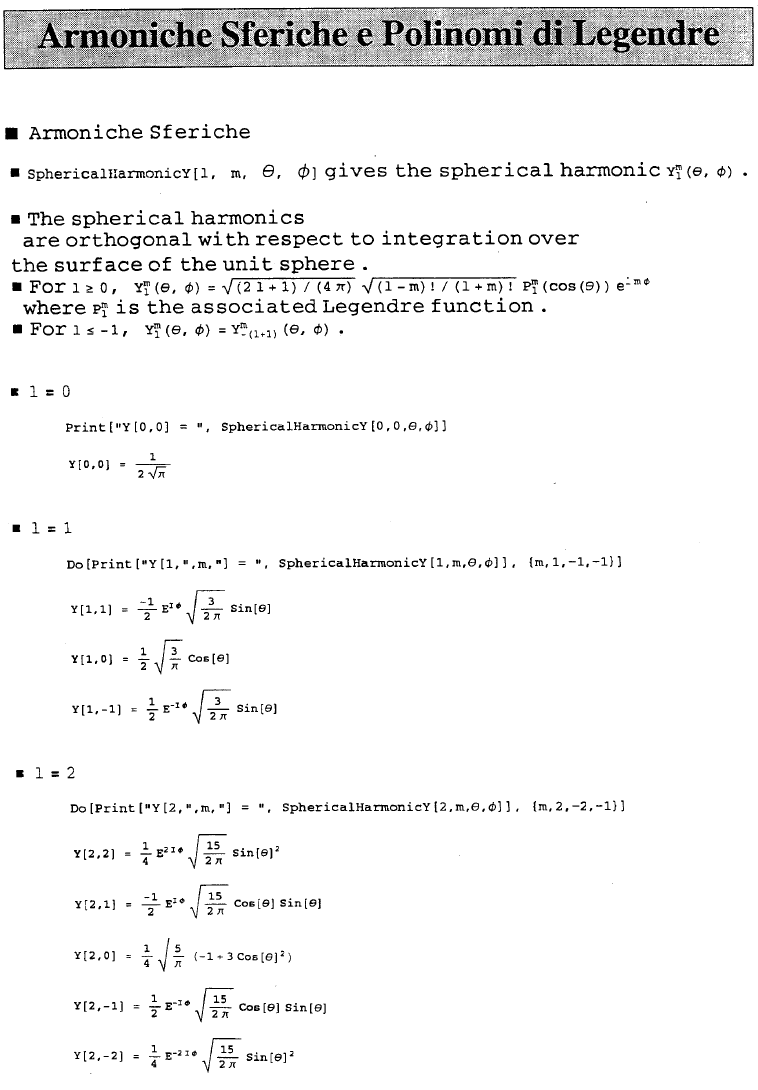
\includegraphics[width=\textwidth]{immagini/cap_17/fig_17_1.png}\\
\end{center}
\end{figure}
\begin{figure}[!htbp]
\begin{center}
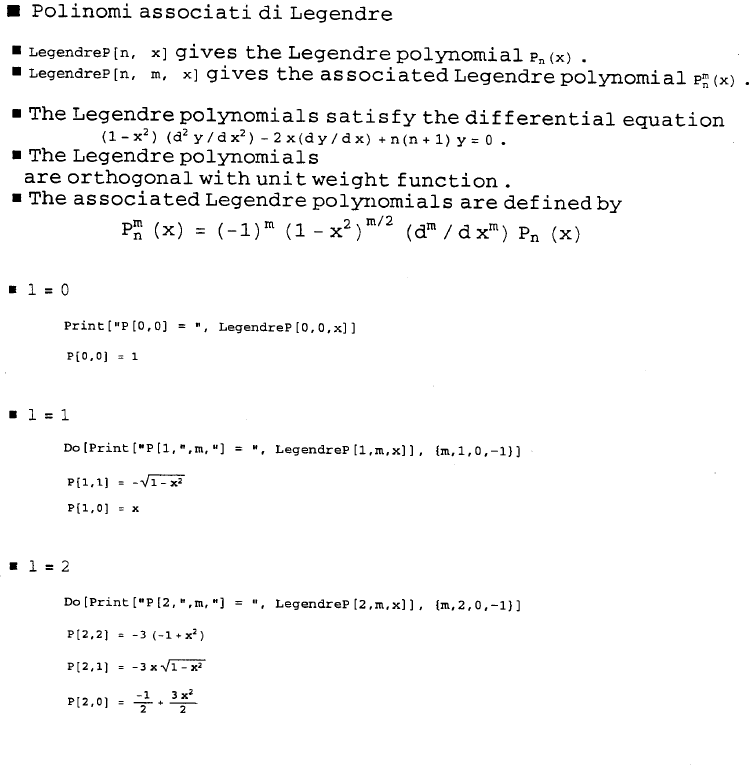
\includegraphics[width=\textwidth]{immagini/cap_17/fig_17_2.png}\\
\end{center}
\end{figure}
 %DEFINITIVO
\chapter{Spin}
Nella meccanica quantistica si deve assegnare ad ogni particella un \textbf{momento angolare intrinseco} non legato con il suo moto nello spazio. Questa \textbf{proprietà} della materia è \textbf{squisitamente quantistica} (essa scompare nel passaggio al limite $\hbar\rightarrow0$) e, di conseguenza, non ammette un'interpretazione classica.\\ Il momento angolare intrinseco di una particella è chiamato \textbf{spin} della particella, a differenza del momento angolare legato al moto della particella nello spazio, che è detto momento angolare orbitale.\\ Lo spin di una particella, misurato in unità $\hbar$, sarà indicato con s. Gli operatori delle componenti del momento angolare di spin, trattandosi di operatori di momento angolare, soddisfano le regole di commutazione
\begin{equation}
[s_{i},s_{j}]=i\varepsilon_{ijk}\hbar s_{k} ,
\label{18.1}
\end{equation}
con tutte le conseguenze fisiche che ne derivano.\\
In particolare gli \textbf{autovalori del quadrato dello spin}, $s^{2}$. sono uguali a:
\begin{equation}
\hbar^{2}s(s+1) ,
\end{equation}
dove \textbf{s può essere o un numero intero(compreso lo zero) o semintero}.\\ \textbf{Per un dato s la componente $s_{z}$ dello spin può prendere i valori}
\begin{equation}
-s, -s+1,.....,s-1,s ,
\end{equation}
\textbf{in unità $\hbar$}, in totale 2s+1 valori.\\ \textbf{Poichè s è per ogni tipo di particella un numero dato, nel passaggio al limite classico ($\hbar\rightarrow0$) il momento angolare di spin $\hbar s$ si annulla}. Per il momento angolare orbitale questo ragionamento non ha senso, poichè \textit{l} può avere valori arbitrari. Il passaggio alla meccanica classica significa che, contemporaneamente $\hbar$ tende a zero ed \textit{l} all'infinito, cosicchè il prodotto $\hbar l$ resta finito.\\ \textbf{Per le particelle aventi uno spin, la descrizione dello stato mediante la funzione d'onda deve determinare non soltanto la probabilità delle sue diverse posizioni nello spazio, ma anche la probabilità delle diverse orientazioni possibili del suo spin}.
In altre parole, la funzione d'onda deve dipendere non soltanto da tre variabili continue, cioè dalle coordinate della particella,ma anche da una variabile di spin discreta che determina il valore della proiezione dello spin su una direzione scelta nello spazio(asse z) e suscettibile di un valore limitato di valori discreti(che indicheremo con la lettera $\sigma$). Tale funzione d'onda si scrive
\begin{equation}
\psi_{\sigma}(\vec{x'})=\langle\vec{x'}, \sigma|\alpha\rangle .
\end{equation} 
Essa rappresenta sostanzialmente un insieme di funzioni delle coordinate, che corrispondono a diversi valori di $\sigma$. Queste funzioni sono dette \textbf{componenti di spin della funzione d'onda}.\\ Frequentemente, le diverse componenti di spin della funzione d'onda sono arrangiate in un vettore colonna:
\[
\begin{pmatrix}
\psi_{\sigma_1}(\vec{x'})\\ \psi_{\sigma_2}(\vec{x'})\\ \vdots \\\psi_{2s+1}(\vec{x'})
\end{pmatrix}
\] 
Il modulo quadro 
\begin{equation}
\vert\psi_{\sigma}(\vec{x'})\vert^{2}  , 
\end{equation}
rappresenta la \textbf{densità di probabilità di trovare la particella nella posizione $\vec{x'}$ con un determinato valore di $\sigma$}. Pertanto la probabilità che la particella abbia un determinato valore di $\sigma$ è determinata dall'integrale
\begin{equation}
\int_{-\infty}^{+\infty} \vert\psi_{\sigma}(\vec{x'})\vert^{2}\,\vec{dx'} .
\end{equation}
Quanto alla probabilità della particella di trovarsi nell'elemento di volume $\vec{dx'}$, ma con un valore arbitrario di $\sigma$, essa è:
\begin{equation}
\sum_{\sigma} \vert\psi_{\sigma}(\vec{x'})\vert^{2}\vec{dx'}  .
\end{equation}
È evidente come, per una particella dotata di spin, la condizione di normalizzazione della funzione d'onda si scrive nella forma:
\begin{equation}
\sum_{\sigma} \int_{-\infty}^{+\infty}\vec{dx'}\vert\psi_{\sigma}(\vec{x'})\vert^{2}=\sum_{\sigma} \int_{-\infty}^{+\infty}\vec{dx'}\langle\alpha|\vec{x'}, \sigma\rangle\langle\vec{x'}, \sigma|\alpha\rangle=1 .
\end{equation}
Questo risultato segue anche dalla relazione di completezza
\begin{equation}
\sum_{\sigma} \int \vec{dx'}|\vec{x'}, \sigma\rangle\langle\vec{x'}, \sigma|=1 ,
\end{equation}
valida per i vettori di stato rappresentativi di particelle con spin.
\section{Operatori di spin e formalismo di Pauli per spin 1/2}
In questo capitolo non ci interesseremo, e non indicheremo pertanto esplicitamente, la dipendenza dalle coordinate spaziali dei vettori di stato.\\
Gli operatori di spin agiscono appunto sulla varietà di spin $\sigma$ e si possono rappresentare in forma di \textbf{matrici di dimensione (2s+1)}.\\
Consideriamo gli elementi di matrice degli operatori di spin nella base in cui il quadrato dello spin $s^{2}$ e la sua componente lungo l'asse z, $s_{z}$, sono diagonali. Questa base è definita dagli autovettori $|s,\sigma\rangle$ che soddisfano:
\begin{eqnarray}
& &s^{2} |s, \sigma\rangle =\hbar^{2}s(s+1)|s, \sigma\rangle ,\\
& &s_{z} |s, \sigma\rangle =\hbar \sigma |s, \sigma\rangle . 
\end{eqnarray}
Gli elementi di matrice degli operatori $s_{x}$ e $s_{y}$ in questa base sono espressi dalle relazioni derivate  nella discussione generale della teoria del momento angolare:
\begin{eqnarray}
& &\langle s, \sigma -1\vert s_{x}\vert s, \sigma\rangle = \langle s, \sigma\vert s_{x}\vert s, \sigma -1\rangle =\frac{\hbar}{2}\sqrt{s(s+1)-\sigma(\sigma-1)} , \nonumber \\
\\
& &\langle s, \sigma -1\vert s_{y}\vert s, \sigma\rangle =- \langle s, \sigma\vert s_{y}\vert s, \sigma -1\rangle =\frac{i\hbar}{2}\sqrt{s(s+1)-\sigma(\sigma-1)} . \nonumber \\
\end{eqnarray}
Nel caso più importante in cui lo \textbf{spin} è uguale a \textbf{1/2} le matrici rappresentative degli operatori di spin hanno dimensione 2 e sono della forma
\begin{equation}
\vec{s}\doteq\frac{\hbar}{2}\vec{\sigma} ,
\end{equation}
dove
\begin{equation}
\sigma_{x}=\begin{pmatrix}
0 & 1 \\
1 & 0
\end{pmatrix}, \qquad \sigma_{y}=\begin{pmatrix}
0 & -i \\
i & 0
\end{pmatrix},\qquad \sigma_{z}=\begin{pmatrix}
1 & 0 \\
0 & -1
\end{pmatrix},
\end{equation}
le matrici $\vec{\sigma}$ si chiamano \textbf{matrici di Pauli}.\\
In accordo con le regole (\ref{18.1}), le matrici di Pauli soddisfano le \textbf{relazioni di commutazione}
\begin{equation}
[\sigma_{i}, \sigma_{j}]=2i\varepsilon_{ijk}\sigma_{k} .
\end{equation}
Possiamo inoltre derivare con un calcolo diretto, le seguenti proprietà specifiche delle matrici di Pauli
\begin{equation}
\sigma_{i}^{2}=1, \quad \sigma_{i}\sigma_{j}+\sigma_{j}\sigma_{i}=0 \quad per \; i \neq j .
\end{equation}
Queste relazioni sono ovviamente equivalenti alle \textbf{relazioni di anticommutazione}\footnote{Tutte queste proprietà sono riassunte dall'unica relazione $\sigma_{i}\sigma_{j}=\delta_{ij}+i\varepsilon_{ijk}$}:
\begin{equation}
\lbrace\sigma_{i}, \sigma_{j}\rbrace=2\delta_{ij}
\end{equation}
Quanto all'operatore $s^{2}$, la sua rappresentazione in questa base risulta:
\begin{equation}
s^{2}=s_{x}^{2}+s_{y}^{2}+s_{z}^{2}=\frac{\hbar^{2}}{4}(\sigma_{x}^{2}+\sigma_{y}^{2}+\sigma_{z}^{2})=
\frac{3}{4}\hbar^{2}\doteq\frac{3}{4}\begin{pmatrix}
1 & 0 \\
0 & 1
\end{pmatrix} ,
\end{equation} 
in accordo con il fatto che per una particella di spin 1/2 gli autostati $\vert s, \sigma\rangle$ sono autostati  dell'operatore $s^{2}$ con autovalore $\hbar^{2}s(s+1)=\frac{3}{4}\hbar^{2}$.\\
Gli autostati $\vert s, \sigma\rangle$ per una particella di spin 1/2 corrispondenti agli autovalori $\sigma=\pm\hbar/2$ vengono frequentemente indicati con i simboli $\vert +\rangle$ e $\vert -\rangle$ (o anche $\vert \uparrow \rangle$ e $\vert \downarrow \rangle$). Quanto alla loro rappresentazione matriciale nella base da essi stessi costituita questa è ovviamente
\begin{equation}
\vert +\rangle\doteq\begin{pmatrix}
1 \\
0
\end{pmatrix}\equiv \chi_{+}\;, \qquad \vert - \rangle\doteq\begin{pmatrix}
0 \\
1
\end{pmatrix}\equiv \chi_{-} ,
\end{equation}
e per i corrispondenti vettori bra:
\begin{equation}
\langle + \vert \doteq \begin{pmatrix}
1 & 0
\end{pmatrix} \equiv \chi_{+}^{+} \; , \qquad \langle - \vert \doteq \begin{pmatrix}
0 & 1
\end{pmatrix} \equiv \chi_{-}^{+} .
\end{equation}
Un generico vettore di stato $\vert \alpha \rangle$ è esprimibile come combinazione lineare dei due stati di base $\vert + \rangle$ e $\vert - \rangle$ nella forma:
\begin{equation}
\alpha = c_{+}\vert + \rangle + c_{-}\vert - \rangle\doteq \begin{pmatrix}
c_{+}\\
c_{-}
\end{pmatrix}= c_{+}\chi_{+}+c_{-}\chi_{-} ,
\end{equation}
dove i coefficienti complessi corrispondono alle ampiezze di probabilità
\[
c_{+}=\langle + \vert \alpha \rangle \; , \qquad c_{-}=\langle - \vert \alpha \rangle .
\]
Il vettore colonna $\begin{pmatrix}
c_{+}\\
c_{-}
\end{pmatrix}$ è chiamato \textbf{spinore} a due componenti.%DEFINITIVO
\chapter[Composizione di momenti angolari]{Composizione di momenti angolari\footnote{S3.7, LL31}}
Consideriamo un sistema composto da due parti. Il momento angolare totale di questo sistema, $\vec{J}$, può essere scritto come la somma dei momenti angolari $\vec{J_1}$ e $\vec{J_2}$ delle sue parti:
\begin{align} \label{eq:cap19_01}
\vec{J} = \vec{J_1} + \vec{J_2}.
\end{align}
Se le due parti che costituiscono il sistema interagiscono tra loro, la legge di conservazione del momento angolare si applica soltanto al momento angolare totale $\vec{J}$, e non ai momenti angolari $\vec{J_1}$ e $\vec{J_2}$ presi separatamente.\\
Considerazioni analoghe possono essere effettuate per un sistema con momento angolare di spin $\vec{S}$ diverso da zero. Per un tale sistema la legge di conservazione del momento angolare si applica (in generale) soltanto al momento angolare totale del sistema, composto dalla componente orbitale e dalla componente di spin:
\begin{equation}
\vec{J} = \vec{L} + \vec{S}.
\end{equation}
Nello studio di tali sistemi si pone il problema della legge di composizione dei momenti angolari. Quali sono i valori possibili di $j$ dati i valori di $j_1$ e $j_2$? \\
Quanto alla legge di composizione delle proiezioni del momento angolare, essa è evidente: dal fatto che $J_z = J_{1z} + J_{2z}$ segue che 
\begin{equation} \label{eq:cap19_02}
m= m_1 + m_2.
\end{equation}
Per dedurre la legge di composizione dei quadrati dei momenti angolari ragioniamo nel modo seguente: prendiamo come sistema completo di grandezze fisiche le grandezze
\begin{equation}
J_1^2 ,~ J_2^2 ,~ J_{1z} ,~ J_{2z} ,
\end{equation}
e una serie di altre grandezze che, con le quattro indicate, costituiscono un sistema completo. Poichè queste altre grandezze non intervengono nei ragionamenti successivi, per abbreviare le espressioni non le considereremo affatto.\\
Ogni stato sarà determinato allora dai numeri $j_1 , ~ j_2 ,~ m_1 , ~ m_2$ e lo indicheremo pertanto con
\begin{equation}
| j_1 , ~ j_2 ,~ m_1 ,~ m_2 \rangle .
\end{equation}
Per $j_1$ e $j_2$, i numeri $m_1$ e $m_2$ assumono rispettivamente $(2 j_1 + 1)$ e $(2 j_2 + 1)$ 
valori, cosicché si hanno in tutto
\begin{equation} \label{eq:cap19_03}
N= (2j_1 + 1) (2j_2 + 1) 
\end{equation}
stati diversi con gli stessi $j_1$ e $j_2$. \\
In luogo delle quattro grandezze indicate si possono prendere anche. come sistema completo, le quattro grandezze:
\begin{equation}
J^2 ,~ J_z ,~ J_1^2 ,~ J_2^2 . 
\end{equation}
Si trova infatti che, ad esempio, l'operatore $J_1^2$  commuta con $J_2^2$, come risulta evidente dall'espressione:
\begin{align}
J^2 = (\vec{J_1} + \vec{J_2})^2 = J_1^2 + J_2^2 + 2 (J_{1x} J_{2x} + J_{1y} J_{2y} + J_{1z} J_{2z}),
\end{align}
(sottolineiamo che gli operatori $\vec{J_1}$ e $\vec{J_2}$, agendo sui diversi sottospazi, commutano tra loro).\\
 In questo caso ogni stato sarà caratterizzato da valori dei numeri $j, ~  m, ~ j_1,~  j_2$ e lo indicheremo con
\begin{center}
$| j ,~ m,~j_1, ~ j_2 \rangle $ .
\end{center}
Dati $j_1$ e $j_2$ si debbono avere, ovviamente, come prima $N = (2j_1+1)(2j_2+1)$ stati diversi, cioè dati $j_1$ e $j_2$ la coppia di numeri $j$ ed $m$ può prendere $(2j_1+1)(2j_2+1)$ coppie di valori. Il ragionamento seguente permette di determinare questi valori.\\
Il valore massimo possibile di $m$, in accordo con l'eq. \eqref{eq:cap19_02}, è $m = j_1 + j_2$ e a questo corrisponde un solo stato $| j_1 ,~ j_2,~m_1, ~ m_2 \rangle $ (coppia di valori $m_1$, $m_2$). Pertanto, il valore massimo possibile di m negli stati $\mid j ,~ m,~j_1, ~ j_2 > $  e, di conseguenza, il valore massimo di $j$ è $j_1 + j_2$. 

\begin{center}
\begin{tabular}{c||c|c||c|c||c}

	& 	$m_1$&	$m_2$&	$m$&	$j$\\
\cline{2-5}
\cline{2-5}
	1)&	$j_1$&	$j_2$&	$j_1+j_2$&	$j_1+j_2$&\\
	
\cdashline{2-5}
\end{tabular}
\end{center}
Esistono inoltre due stati i $| j_1 ,~ j_2,~m_1, ~ m_2 \rangle $ con $m= j_1 + j_2 -1$. Di conseguenza, ci debbomo essere ugualmente due stati $| j ,~ m,~j_1, ~ j_2 \rangle $ con questo valore di m. Uno di essi è lo stato con $j= j_1 + j_2$ (con $m=j-1$) e l'altro con $j= j_1+ j_2 -1$ (per $m=j$)
\begin{center}
\begin{tabular}{c||c|c||c|c||c}

	& 	$m_1$&	$m_2$&	$m$&	$j$\\
\cline{2-5}
\cline{2-5}
	1)&	$j_1$&	$j_2-1$&	\multirow{2}{*}{$j_1+j_2-1$}&	$j_1+j_2$	&1)\\ \hhline{~--~-~}
	2)&	$j_1-1$&	$j_2$&	&$j_1+j_2-1$	&2)\\	
\cdashline{2-5}
\end{tabular}
\captionof*{table}{\textit {~~Stati~$| j_1 ,~ j_2,~m_1, ~ m_2 \rangle $~~~~~~~~Stati~$| j ,~ m,~j_1, ~ j_2 \rangle $}}
\end{center}
Per il valore $m= j_1 + j_2 -2$ esistono tre diversi stati $| j_1 ,~ j_2,~m_1, ~ m_2 \rangle $. Ciò significa che oltre ai valori $j= j_1 + j_2, j= j_1 + j_2 -1$ è possibile anche il valore $j= j_1 +j_2 -2$. \\

\begin{center}
\begin{tabular}{c||c|c||c|c||c}

	& 	$m_1$&	$m_2$&	$m$&	$j$\\
\cline{2-5}
\cline{2-5}
	1)&	$j_1$&	$j_2-2$&	\multirow{3}{*}{$j_1+j_2-2$}&	$j_1+j_2$	&1)\\ \hhline{~--~-~}
	2)&	$j_1-1$&	$j_2-1$&	&$j_1+j_2-1$	&2)\\	\hhline{~--~-~}
	3)&	$j_1-2$&	$j_2$&	&$j_1+j_2-2$	&3)\\
\cdashline{2-5}
\end{tabular}
\captionof*{table}{\textit {~~Stati~$| j_1 ,~ j_2,~m_1, ~ m_2 \rangle $~~~~~~~~Stati~$| j ,~ m,~j_1, ~ j_2 \rangle $~}}
\end{center}
Questo ragionamento si può continuare nello stesso modo finché diminuendo m di 1 aumenta di 1 il numero di stati con il dato valore di m. E' facile capire che ciò si verifica finché, assumendo ad esempio $j_1 \geq j_2$,m non raggiunge il valore $j_1-j_2$. Diminuendo ulteriormente m, il numero di stati cessa di crescere, restando uguale a $2j_2+1$; il valore di $m_2$ infatti, non può essere minore di $-j_2$. Ciò significa che $j_1-j_2$, o in generale $|j_1-j_2|$, è il valore minimo possibile di $j$. \\
Così siamo giunti al risultato che, dati $j_1$ e $j_2$, il numero $j$ può prendere i valori:  
\begin{equation} \label{eq:cap19_04}
j= |j_1-j_2|, |j_1-j_2|+1, ......, j_1+j_2-1, j_1+j_2,
\end{equation}
 cioè in totale $2j_2 + 1$ valori diversi (supponendo che $j_2 \leq j_1$).  \\
Tenendo conto per ogni valore di $j$ esistono $(2j+1)$ stati $| j ,~ m,~j_1, ~ j_2 \rangle $  corrispondenti ai diversi possibili valori di $m$ possiamo verificare che il numero totale di stati è (per $j_2 \leq j_1$):
\begin{align}
N~ &= \sum_{j=j_1-j_2}^{j_1+j_2}{(2_j + 1)} = \nonumber \\
&= \sum_{k=0}^{2j_2}{[2(k+j_1-j_2)+1]}= \nonumber \\
&= 2 \sum_{k=0}^{2j_2}{k} + [2(j_1-j_2)+1](2j_2+1) =\nonumber \\
&= 2j_2(2j_2+1)+[2(j_1-j_2)+1](2j_2+1) = \nonumber \\ \nonumber \\
&= (2j_1+1)(2j_2+1)
\end{align}
in accordo con il risultato (\ref{eq:cap19_03}).\\
Il risultato ottenuto per i possibili valori di $j$ (eq.(\ref{eq:cap19_04})) può essere illustrato mediante il cosiddetto \emph{modello vettoriale}. Se introduciamo due vettori $\vec{J_1}$ e $\vec{J_2}$ con moduli $j_1$ e $j_2$, i valori di $j$ saranno rappresentati come moduli interi dei vettori $\vec{J}$, ottenuti componendo vettorialmente i $\vec{J_1}$ e $\vec{J_2}$. Il valore massimo $(j_1+j_2)$ di $j$ si ottiene allorché $\vec{J_1}$ e  $\vec{J_2}$ sono paralleli, e il valore minimo $(|j_1-j_2|)$ allorché essi sono antiparalleli.
%%%%%%%%%%%%%%%%%%%%%%%%%%%%%%%%%%%%%%%%%%%%%%%%%%%%%%5
\section[Coefficienti di Clebsh-Gordan]{Coefficienti di Clebsh-Gordan\footnote{S3.7}}
Consideriamo la trasformazione unitaria che connette la base degli autostati di $J_1^2 ,~ J_2^2 ,~ J_{1z} ,~ J_{2z}$ alla base degli autostati di  $J^2 ,~ J_z ,~ J_1^2 ,~ J_2^2$.
\begin{align} \label{eq:cap19_05}
| j ,~ m,~j_1, ~ j_2 \rangle  = \sum_{m_1, m_2} {| j_1 ,~ j_2,~m_1, ~ m_2 \rangle \langle j_1 ,~ j_2,~m_1, ~ m_2 |  j ,~ m,~j_1, ~ j_2 \rangle }.
\end{align}
Per scrivere questa relazione abbiamo utilizzato la relazione di completezza
\begin{align}
\sum_{m_1, m_2} {| j_1 ,~ j_2,~m_1, ~ m_2 \rangle \langle j_1 ,~ j_2,~m_1, ~ m_2 | = 1 },
\end{align}
dove il secondo membro è l'operatore di identità nello spazio dei vettori di stato con $j_1$ e $j_2$ assegnati. \\
Gli elementi di matrice unitaria che effettua il cambiamento di base, ossia la grandezza
\begin{equation}
\langle j_1 ,~ j_2,~m_1, ~ m_2 ~|~ j ,~ m,~j_1, ~ j_2 \rangle ,
\end{equation}
sono detti \textbf{coefficienti di Clebsh-Gordan}.\\
Dalle leggi di composizione del momento angolare totale e della sua componente $z$ segue ovviamente che i coefficienti di C.G. sono zero a meno che
\begin{equation}
m=m_1+m_2\quad \textrm{e}\quad |j_1-j_2| \leq j \leq j_1+j_2.
\end{equation}
Per convenzione, i coefficienti di C.G. sono definiti reali:
\begin{align}
\langle j_1 ,~ j_2,~m_1, ~ m_2~ |~ j ,~ m,~j_1, ~ j_2 \rangle  = \langle j ,~ m,~j_1, ~ j_2~ |~ j_1 ,~ j_2,~m_1, ~ m_2 \rangle .
\end{align}
La condizione di ortogonalità degli autostati $\mid j ,~ m,~j_1, ~ j_2 >$ applicata all'eq. (\ref{eq:cap19_05}), unitamente alla condizione di realtà dei coefficienti di C.G., fornisce:
\begin{align}
 \sum_{m_1, m_2} {\langle j_1 , j_2, m_1, m_2 | j' , m', j_1, j_2 \rangle  \langle j_1 , j_2, m_1, m_2  | j , m, j_1, j_2 \rangle } = \delta_{j j'} \delta{m m'},
\end{align}
che coincide con la condizione di unitarietà della matrice dei coefficienti di C.G.. In particolare, per $j=j'$ ed $m=m'$ si ottiene:
\begin{align}
 \sum_{m_1, m_2} {|\langle j_1 ,~ j_2,~m_1, ~ m_2 ~|~ j ,~ m,~j_1, ~ j_2 \rangle|^2} =1 , 
\end{align}
che non è altro che la condizione di normalizzazione degli stati $| j ,~ m,~j_1, ~ j_2 \rangle $. \\
Un metodo conveniente per determinare i coefficienti di C.G. consiste nell'utilizzare gli operatori a scala secondo la seguente procedura. \\
Nella composizione di due momenti angolari $\vec{J_1}$ e  $\vec{J_2}$ lo stato corrispondente al valore massimo della componente $z$ del momento angolare, ossia $m= j_1+j_2$ e dunque $j=j_1+j_2$ coincide necessariamente, a mo' di un fattore di fase, con lo stato avente $m_1=j_1$ ed $m_2=j_2$. Il fattore di fase è posto per convenzione uguale ad 1. Allora
\begin{align}
| j= j_1 + j_2 ,~m= m_1 +m_2  \rangle ~= ~| j_1 ,~j_2,  m_1=j_1, ~m_2= j_2 \rangle .
\end{align}
Applicando ad entrambi i membri di questa equazione l'operatore $J=J_1+J_2$ si può determinare lo stato con $j=j_1+j_2$ ed $m=j_1+j_2-1$ in termini degli stati con $(m_1=j_1-1 , m_2=j_2)$ e $(m_1=j_1, m_2=j_2-1)$. Lo stato con lo stesso valore di $m$ ma $j=j_1+j_2-1$ è poi costruito imponendo l'ortogonalità con il precedente. In questo modo si possono determinare tutti i coefficienti di C.G. del sistema considerato. \\
Consideriamo questa procedura discutendo un esempio specifico importante.
%%%%%%%%%%%%%%%%%%%%%%%%%%%%%%%%%%%%%%%%%%%%%%%%
\section[Composizione di due momenti angolari di spin 1/2. Stati di tripletto e di singoletto]{Composizione di due momenti angolari di spin 1/2. Stati di tripletto e di singoletto\footnote{S3.7}}
Consideriamo la composizione angolare di sin per due particelle di spin 1/2. Il momento angolare di spin totale delle due particelle,
\begin{equation}
\vec{S} = \vec{S_1} + \vec{S_2} ,
\end{equation}
può assumere in questo caso solo due valori, corrispondenti ad:
\begin{equation}
S~= ~0, ~1 ,
\end{equation}
in accordo con la legge di composizione (\ref{eq:cap19_04}).\\
Nella base degli autostati comuni degli operatori $S_1^2 ,~ S_2^2, ~ S_{1z}, ~ S_{2z}$ esistono quattro vettori di stato che possiamo indicare con \\ 
\begin{equation}
|++\rangle ,~ |+-\rangle,~ |-+\rangle , ~|--\rangle  ,
\end{equation}
dove, ad esempio, \\
\begin{equation}
|++\rangle~ \equiv ~|s_1=1/2, ~s_2=1/2,~\sigma_1 = 1/2, ~\sigma_2 = 1/2\rangle ,
\end{equation}
e analoghe. \\
Corrispondentemente esistono quattro stati di base corrispondenti agli operatori $S^2 ,~ S_z, ~ S_1^2, ~ S_2^2$. Possiamo indicare questi stati con \\
\begin{equation}
|1,1\rangle, ~|1,0\rangle, ~|1,-1\rangle, ~|0,0\rangle ,
\end{equation}dove \\
\begin{equation}
|1,1\rangle ~\equiv~ |s=1, ~ \sigma=1, ~s_1=1/2, ~s_2=1/2\rangle ,
\end{equation}
ecc... \\
Gli stati corrispondenti a momento angolare di spin $S=1$ sono detti \emph{stati di tripletto}. Lo stato corrispondente a momento angolare di spin $S=0$ \emph{stato di singoletto}. \\
Calcoliamo i coefficienti di C.G. che consentono di esprimere gli autostati di $S^2$ ed $S_z$ in termini degli autostati di $S_1^2 ,~ S_{1z}, ~ S_2^2, ~ S_{2z}$. \\
Lo stato $\sigma=1$ si può ottenere solo per $\sigma_1=\sigma_2=1/2$. \\
Pertanto:\\
\begin{equation}
|1,1\rangle = |++\rangle  .\\
\end{equation}
Applichiamo ora ad entrambi i membri di questa equazione l'operatore a scala $S_-$:
\begin{align}
 S_1 |1,1\rangle & = \sqrt{s(s+1) - \sigma(\sigma -1)}  |1,0\rangle =\sqrt{2}  |1,0\rangle= \nonumber \\
&= (S_1+S_2)  |+,+\rangle = \nonumber \\
&= \sqrt{1/2 (1/2+1) -1/2 (1/2-1)} ( |+,-\rangle + |-,+\rangle)= \nonumber \\
&= |+,-\rangle   +   |-,+\rangle ,
\end{align}
ossia
\begin{equation}
|1,0\rangle = \frac{1}{\sqrt{2}} (|+-\rangle + |-+\rangle) .
\end{equation}
Lo stato $|1,-1\rangle$ si può ottenere mediamente una seconda applicazione dell'operatore a scala. Ma in questo caso si ottiene evidentemente:
\begin{equation}
|1,-1\rangle = |--\rangle .
\end{equation}
Infine, lo stato $|0,0\rangle$ si può ottenere imponendo l'ortogonalità con lo stato $|1,0\rangle$. S trova allora:
\begin{equation}
|0,0\rangle = \frac{1}{\sqrt{2}} (|+-\rangle - |-+\rangle). \\
\end{equation}
In definitiva, abbiamo trovato:

\begin{align}
\begin{cases} 
|1,1\rangle = |++\rangle \nonumber \\
|1,0\rangle = \frac{1}{\sqrt{2}} (~|+-\rangle + |-+\rangle ~)  \nonumber  & \mbox{\textrm{\textbf{Tripletto}}} \\
|1,-1\rangle = |--\rangle  \nonumber \\
\end{cases}
\end{align}

\begin{align}
\begin{cases} 
|0,0\rangle = \frac{1}{\sqrt{2}} (~|+-\rangle - |-+\rangle~) \nonumber  & \mbox{\textrm{\textbf{Singoletto}}}\\
\end{cases}
\end{align}

%%%%%%%%%%%%%%%%%%%%%%%%%%%%%%%%%%%%%%%%%%%%%%%%%%%%%

\section[Composizione dei momenti angolari orbitale e di spin per una particella di spin 1/2]{Composizione dei momenti angolari orbitale e di spin per una particella di spin 1/2\footnote{S3.7}}

Consideriamo la composizione del momento angolare orbitale e del momento angolare di spin per una particella di spin 1/2.\\
Se  la particella si trova in un autostato del quadrato del momento angolare orbitale $L$ corrispondente all'autovalore $\hbar^2l(l+1)$, allora i valori possibili per il numero quantico $j$, corrispondente al momento angolare totale $\vec{J}=\vec{L}+\vec{S}$ sono dati da:
\begin{equation}
j =  l \pm 1/2 , ~~~~~~~~~(l>0)
\end{equation}
(il caso $l=0$, ossia assenza di momento angolare orbitale, corrisponde a $\vec{J}=\vec{S}$ e non verrà qui considerato).\\
\\
Determiniamo i coefficienti di Clebsch-Gordan che definiscono lo sviluppo delle autofunzioni $\mathcal{Y}_{j,j_z}$ di $J^2$ e $J_z$ in termini delle autofunzioni $Y_{l,m}$ di $L^2$, $L_z$ e $\chi_\pm$ di $S^2$ ed $S_z$.\\
La proiezione:
\begin{gather}
j_z = m + m_s ,\\
(m_s=\pm1/2)~~,~~(m=-l,-l+1,...,l),
\end{gather}
del momento angolare totale può assumere solo valori seminteri. In particolare, un determinato valore $j_z=m+1/2$ può essere ottenuto solo dalle combinazioni $l_z=m$, $s_z=1/2$ o $l_z=m+1$, $s_z=-1/2$. Devono allora valere gli sviluppi ortogonali:
\begin{align} \label{eq:cap19_06}
\begin{cases} 
\mathcal{Y}_{j=l+1/2,~ j_z=m+1/2} = c_+Y_{l,m}\chi_+ + c_-Y_{l, m+1}\chi_- \\
\mathcal{Y}_{j=l-1/2,~ j_z=m+1/2} = -c_-Y_{l,m}\chi_+ + c_+Y_{l, m+1}\chi_- 
\end{cases}
\end{align}
$c_\pm$ rappresentano i coefficienti di Clebsch-Gordan cercati.\\
Per determinare questi coefficienti, consideriamo in partenza lo stato in cui la proiezione $J_z$ del momento angolare totale assume il suo valore massimo: $j_z=l+1/2$. Questo stato corrisponde evidentemente alla combinazione:
\begin{equation} \label{eq:cap19_07}
 \mathcal{Y}_{j=l+1/2,~j_z=l+1/2} = Y_{l,l} \chi_+ .
\end{equation}
Applichiamo ad entrambi i membri di questa equazione l'operatore a scala $J_- = L_-+S_-$.\\
Ricordando il risultato:
\begin{align} \label{eq:cap19_08}
J_-~ \mathcal{Y}_{j,j_z} &= \sqrt{j(j+1)-j_z(j_z-1)}~\mathcal{Y}_{j,j_z-1} = \\ \nonumber
&= \sqrt{(j+j_z)(j-j_z+1)}~\mathcal{Y}_{j,j_z-1} ,
\end{align}
(e le espressioni analoghe per $L_-$ ed $S_-$), otteniamo dal primo membro dell'eq. (\ref{eq:cap19_07}) :
\begin{equation} \label{eq:cap19_09}
J_-~ \mathcal{Y}_{j=l+1/2,~j_z=l+1/2} = \sqrt{2l+1}~\mathcal{Y}_{j=l+1/2,~j_z=l-1/2} .
\end{equation}
Per ottenere l'autofunzione corrispondente a $j_z=m+1/2$ dobbiamo applicare l'operatore $J_-$ $(l-m)$ volte. Una seconda applicazione di $J_-$ all'equazione (\ref{eq:cap19_09}) fornisce:
\begin{align}
(J_-)^2~&\mathcal{Y}_{j=l+1/2,~j_z=l+1/2} = \sqrt{(2l+1)}~J_-~\mathcal{Y}_{j=l+1/2,~j_z=l-1/2} = \nonumber \\
=~ &\sqrt{(2l+1)\cdot 2 \cdot 2l}~\mathcal{Y}_{j=l+1/2,~j_z=l-3/2},
\end{align}
ed una terza applicazione di $J_-$ conduce a:
\begin{align}
(J_-)^3&~\mathcal{Y}_{j=l+1/2,~j_z=l+1/2} = \sqrt{2\cdot(2l+1)\cdot 2l}~J_-~\mathcal{Y}_{j=l+1/2,~j_z=l-3/2} = \nonumber\\
=~&\sqrt{2\cdot 3\cdot(2l+1) \cdot (2l) \cdot (2l-1)}~\mathcal{Y}_{j=l+1/2,~j_z=l-5/2}.
\end{align}
Risulta allora chiaro come il coefficiente che si ottiene applicando $J_-$ un numero $k$ di volte sulla autofunzione iniziale $\mathcal{Y}_{j=l+1/2,~j_z=l+1/2}$ sia:
\begin{equation}
\sqrt{2\cdot 3\cdot~...\cdot k~(2l+1) \cdot (2l) \cdot ~...\cdot(2l+2-k)} = \sqrt{\frac{k! (2l+1)!}{(2l+1-k)!}},
\end{equation}
ossia
\begin{equation} \label{eq:cap19_10}
(J_-)^k~\mathcal{Y}_{j=l+1/2,~j_z=l+1/2} = \sqrt{\frac{k! (2l+1)!}{(2l+1-k)!}}~\mathcal{Y}_{j=l+1/2,~j_z=l+1/2-k}.
\end{equation}
In particolare, scegliendo $k=l-m$, si trova:
\begin{equation} \label{eq:cap19_11}
(J_-)^{l-m}~\mathcal{Y}_{j=l+1/2,~j_z=l+1/2} = \sqrt{\frac{(l-m)! (2l+1)!}{(l+m+1)!}}~\mathcal{Y}_{j=l+1/2,~j_z=m+1/2}.
\end{equation}
Dobbiamo ora considerare l'applicazione dell'operatore $(J_-)^{l-m} = (L_-+S_-)^{l-m}$ sul secondo membro dell'eq. (\ref{eq:cap19_07}).\\
A tale scopo osserviamo che l'applicazione successiva dell'operatore $(S_-)$ un numero $\ge 2$ di volte sullo stato $\chi_+$ produce un risultato nullo:
\begin{equation}
(S_-)^2~\chi_+ = 0
\end{equation}
Si ha pertanto:
\begin{align} \label{eq:cap19_12}
&(L_-+S_-)^{l-m}~Y_{l,l} \chi_+ = [(L_-)^{l-m} + (l-m)(L_-)^{l-m-1}(S_-)]~ Y_{l,l} \chi_+ = \nonumber \\
=~& (L_-)^{l-m}~Y_{l,l} \chi_+ + (l-m)(L_-)^{l-m-1}~Y_{l,l} \chi_- .
\end{align}
L'eq. (\ref{eq:cap19_10}), con la sostituzione $l\rightarrow l-1/2$, ci fornisce direttamente il risultato dell'applicazione dell'operatore $(L_-)^k$ sull'autofunzione $Y_{l,l}$. Si ha:
\begin{equation} \label{eq:cap19_13}
(L_-)^k ~Y_{l,l} = \sqrt{\frac{k!~(2l)!}{(2l-k)!}}~Y_{l,l-k}.
\end{equation}
Utilizzando questo risultato, possiamo allora riscrivere l'eq. (\ref{eq:cap19_12}) nella forma:
\begin{align} \label{eq:cap19_14}
&(L_-+S_-)^{l-m}~Y_{l,l} \chi_+ = \\ \nonumber
&= \sqrt{\frac{(l-m)!~(2l)!}{(l+m)!}}~Y_{l,m} \chi_+ + (l-m)~\sqrt{\frac{(l-m-1)!~(2l)!}{(l+m+1)!}}~Y_{l,m+1} \chi_- .
\end{align}
I coefficienti di Clebsch-Gordan definiti dall'eq. (\ref{eq:cap19_06}) si ottengono in definitiva applicando ad entrambi i membri dell'eq. (\ref{eq:cap19_07}) l'operatore $(J_-)^{l-m}=(L_-+S_-)^{l-m}$ ed utilizzando i risultati (\ref{eq:cap19_11}) e (\ref{eq:cap19_14}). In tal modo si trova:
\begin{align}
&c_+ = \sqrt{\frac{(l-m)!~(2l)!}{(l+m)!}} \cdot \sqrt{\frac{(l+m+1)!}{(l-m)!~(2l+1)!}} = \sqrt{\frac{l+m+1}{2l+1}}, \\
&c_- = \sqrt{\frac{(l-m-1)!~(2l)!}{(l+m+1)!}} \cdot \sqrt{\frac{(l+m+1)!}{(l-m)!~(2l+1)!}} = \sqrt{\frac{l-m}{2l+1}}.
\end{align}
da cui risulta:
\begin{align}
\mathcal{Y}_{j=l+1/2,~ j_z=m+1/2} = \sqrt{\frac{l+m+1}{2l+1}}~Y_{l,m}~\chi_+ + \sqrt{\frac{l-m}{2l+1}}~Y_{l, m+1}~\chi_-, \\
\mathcal{Y}_{j=l-1/2,~ j_z=m+1/2} = -\sqrt{\frac{l-m}{2l+1}}~Y_{l,m}~\chi_+ + \sqrt{\frac{l+m+1}{2l+1}}~Y_{l, m+1}~\chi_-. 
\end{align}
\`E immediato verificare come queste autofunzioni siano ortogonali tra loro e correttamente normalizzate.%DEFINITIVO
\chapter[Particelle identiche]{Particelle identiche\footnote{S6.1,6.2,6.3; LL61,62, G8}}
Nella meccanica classica le particelle identiche (per esempio, elettroni), malgrado l'identità delle loro proprietà fisiche, non perdono però una loro "individualità": si può immaginare di numerare in un certo istante le particelle di un sistema fisico dato e seguire poi il moto di ciascuna di esse lungo la sua traiettoria; sarà allora possibile identificare la particella in qualsiasi istante.\\ 
Nella meccanica quantistica, invece, la situazione \`e completamente diversa. In virtù del principio di indeterminazione, il concetto di traiettoria della particella perde completamente significato. Di conseguenza, localizzate e numerate le particelle ad un certo istante, questo non ci dà la possibilità di identificarle negli istanti successivi.\\
Cos\`i nella meccanica quantistica non esiste, in linea di principio, alcuna possibilità di seguire separatamente ciascuna delle particelle identiche, e quindi di distinguerle. L'identità delle particelle relativa alle loro proprietà fisiche ha quindi un significato molto profondo: essa porta all'indistinguibilità totale delle particelle.\\
Questo principio di indistinguibilità delle particelle identiche ha un ruolo fondamentale nella teoria quantistica dei sistemi formati da particelle identiche.\\
Consideriamo, per iniziare, un sistema formato da due sole particelle identiche. Siano $|a\rangle$, $|b\rangle$,... i vettori di stato di ciascuna particella considerato solo come un sistema dinamico. Possiamo ottenere un vettore di stato per il sistema costituito dalle due particelle prendendo il prodotto di ket per ciascuna particella considerata da sola. Per esempio:
\begin{equation}
|a\rangle|b\rangle,
\label{eq:cap20_1}
\end{equation}
rappresenta lo stato in cui la prima particella si trova nello stato a e la seconda particella nello stato b.\\
Nella \ref{eq:cap20_1} possiamo scambiare il ruolo delle due particelle e ottenere un altro vettore di stato per il sistema costituito dalle due particelle, ossia il vettore di stato:\\
\begin{equation}
|b\rangle|a\rangle.
\label{eq:cap20_2}
\end{equation}
Questo rappresenta lo stato in cui la prima particella si trova nello stato $|b\rangle$,e la seconda nello stato $|a\rangle$.\\
Il processo di scambiare tra loro le due particelle è un operatore lineare che può essere applicato ai vettori di stato del sistema costituito dalle due particelle. Indicando con $P_{12}$ questo operatore si ha ad esempio:
\begin{equation}
P_{12}|a\rangle|b\rangle = |b\rangle|a\rangle.
\end{equation}
Supponiamo di effettuare una misura sul sistema costituito dalle due particelle, e di trovare che una particella si trova nello stato a e l'altra nello stato b, Tuttavia non sappiamo a priori se lo stato sia $|a\rangle|b\rangle$ o $|b\rangle|a\rangle$ oppure una qualsiasi combinazione lineare dei due, della forma:
\begin{equation}
|\psi\rangle = C_1|a\rangle|b\rangle + C_2 |b\rangle|a\rangle.
\label{eq:cap20_3}
\end{equation}
In altri termini, tutti i vettori di stato della forma \ref{eq:cap20_3} portano allo stesso insieme di autovalori quando si esegue la misura. Ciò è noto come \textbf{degenerazione di scambio}.\\
La degenerazione di scambio sembra rappresentare una difficoltà, poiché, contrariamente al caso di una particella singola, l'assegnazione degli autovalori di un insieme completo di osservabili non determina completamente il vettore di stato.\\
Tuttavia, \textbf{il principio di indistinguibilità delle particelle identiche implica che gli stati del sistema che si ottengono l'uno dall'altro semplicemente scambiando le due particelle, devono essere fisicamente del tutto equivalenti. Questo significa che, come risultato dello scambio, il vettore di stato del sistema può variare soltanto di un fattore di fase inessenziale.} Ossia:
\begin{equation}
P_{12}|\psi\rangle =  e^{i\alpha}|\psi\rangle,
\end{equation}
dove $\alpha$ è una costante reale.\\
Scambiando ancora una volta le due particelle si deve riottenere, evidentemente, lo stato iniziale. L'operatore $P_{12}$ soddisfa cioè:\\
\begin{equation}
P_{12}^2 = 1.
\end{equation}
L'applicazione dell'operatore $P_{12}^2$ allo stato $|\psi\rangle$ equivale a moltiplicare il fattore di stato per $e^{2i}$. Ne segue che $e^{2i\alpha} = 1 $, ossia $e^{i\alpha}=\pm1$. Di conseguenza:
\begin{equation}
P_{12} |\psi\rangle= \pm |\psi\rangle .
\end{equation}
\textbf{Siamo quindi giunti al risultato fondamentale che esistono in tutto due possibilità: o il vettore di stato di un sistema costituito da due particelle identiche è simmetrico, cioè non cambia nello scambio delle due particelle, o esso è antisimmetrico, cioè nello scambio cambia di segno}. Le due combinazioni corrispondono rispettivamente agli stati:
\begin{eqnarray}
\label{eq:cap20_4}
|\psi\rangle= \frac{1}{\sqrt{2}}\left(|a\rangle |b\rangle + |b\rangle|a\rangle \right) ,\nonumber \\
\\
|\psi\rangle= \frac{1}{\sqrt{2}}\left(|a\rangle |b\rangle - |b\rangle|a\rangle \right). \nonumber
\end{eqnarray}
\textbf{È evidente, inoltre, che i vettori di stato rappresentativi di tutti gli stati dello stesso sistema devono godere della stessa simmetria. Se così non fosse, infatti, il vettore di stato che rappresenta la sovrapposizione di stati con diverse simmetrie, non sarebbe né simmetrico né antisimmetrico}.\\
Questo risultato si generalizza immediatamente ai sistemi formati da un \textbf{numero qualsiasi di particelle identiche}. Infatti, a causa dell'identità delle particelle, è chiaro che se una coppia di queste particelle goda della proprietà di poter essere scritta, per esempio, da vettori di stato simmetrici, tutte le altre coppie di particelle avranno la stessa proprietà. \textbf{Quindi il vettore di stato delle particelle identiche deve o restare o assolutamente immutato per lo scambio di qualsiasi coppia di particelle, o cambiare di segno per lo scambio di ogni coppia.}\\
\textbf{Le proprietà del sistema di poter essere descritto da vettori di stato simmetrici o antisimmetrici dipende dalla natura delle particelle che lo compongono.} Delle particelle descritte da vettori di stato simmetrici, si dice che ubbidiscano alla \textbf{statistica di Bose-Einstein}, o che sono \textbf{bosoni}, delle particelle descritte da vettori di stato antisimmetrici, si dice che ubbidiscano alla \textbf{statistica di Fermi-Dirac}, ovvero che sono \textbf{fermioni}. Così, indicando con $P_{ij}$ l'operatore che scambia la i-esima e la j-esima particella si ha:
\begin{eqnarray}
&P_{ij} |N_{\textrm{bosoni identici}}\rangle= +|N_{\textrm{bosoni identici}}\rangle & \nonumber \\
\\
&P_{ij} |N_{\textrm{fermioni identici}}\rangle= -|N_{\textrm{fermioni identici}}\rangle & \nonumber
\end{eqnarray}
Utilizzando le leggi della meccanica quantistica relativistica è possibile mostrare che l\textbf{a statistica cui obbediscono le particelle è univocamente legata al loro spin: le particelle con spin intero sono bosoni, quelle con spin semintero sono fermioni.}\\
È semplice generalizzare le espressioni \ref{eq:cap20_4} al caso di sistemi con un numero arbitrario di particelle identiche. Nel caso generale di un sistema con un numero arbitrario di \textbf{N bosoni identici}, il vettore di stato normalizzato è:\\
\begin{equation}
|\psi\rangle= \left(\frac{N_{1}! N_{2}!\dots}{N!}\right)^{1/2} \begin{matrix} \sum_{k=1}^N |p^k\rangle_{k} \end{matrix}, \\
\end{equation}
dove $|p^{(k)}\rangle_i$ rappresenta il ket della particella i-esima che si trova nello stato $p^k$, la somma \`e estesa a tutte le permutazioni distinte degli indici $p^{(1)}...p^{(N)}$, ed il numero $N_{k}$ indica quante volte il valore $p^{(k)}$ compare nella combinazione sotto il segno di somma.\\
Per un sistema di \textbf{N fermioni identici} il vettore di stato \`e la combinazione antisimmetrica dei prodotti $|p^1\rangle_1...|p^N\rangle_N$. Questa combinazione pu\`o essere scritta nella forma di determinante:\\
\begin{equation}
|\psi\rangle= \frac{1}{\sqrt{N}} \begin{vmatrix} |p_{1}\rangle_1 & |p_{1}\rangle_2 & ... & |p_{1}\rangle_N \\|p_{2}\rangle_1 & |p_{2}\rangle_2 & ... & |p_{2}\rangle_N \\ ... & ... & ... & ... \\ ... & ... & ... & ... \\ ... & ... & ... & ... \\|p_{N}\rangle_1 & |p_{N}\rangle_2 & ... & |p_{N}\rangle_N\end{vmatrix}.
\label{eq:cap20_5}
\end{equation}
Allo scambio di due particelle corrisponde in questo caso lo scambio di due colonne dal determinante, ciò che causa il cambiamento di segno di quest'ultimo.\\
Dall'espressione \ref{eq:cap20_5} segue un risultato importante: se fra gli indici $p_1, p_2...$ ve ne sono due identici, due righe del determinante risulteranno identiche e quindi esso si annulla identicamente \textbf{Di conseguenza, in un sistema di fermioni identici due (o pi\`u) particelle non possono trovarsi in uno stesso stato.} Questo è il cosiddetto \textbf{principio di Pauli.} Nel caso particolare di un sistema costituito da due soli fermioni identici, ad esempio, l'espressione \ref{eq:cap20_4} mostra come il vettore di stato antisimmetrico si annulla identicamente quando i due fermioni si trovano nello stesso stato: $|a\rangle= |b\rangle$.\\
La proprietà di simmetria di un vettore di stato per un sistema di particelle identiche deve conservarsi invariata nel tempo. Così, ad esempio, un vettore di stato simmetrico all'istante iniziale t=0, deve risultare simmetrico a qualunque istante di tempo successivo. \textbf{Questa circostanza è garantita dal fatto che l'operatore hamiltoniano per un sistema composto da N particelle identiche commuta con l'operatore di scambio $P_{i}$ di una coppia qualunque di particelle i e j del sistema:}\\
\begin{equation}
\left [ H, P_{ij}\right ]=0
\end{equation}
Per dimostrare questa relazione limitiamoci a considerare, per semplicit\`a, un sistema costituito da una sola coppia di particelle identiche. Indichiamo poi con $\xi_{1}$ e $\xi_{2}$ gli insiemi delle tre coordinate e della proiezione dello spin di ciascuna delle particelle. Possiamo allora introdurre la funzione d'onda del sistema:\\
\begin{equation}
|\psi_{\alpha}(\xi_1 \xi_2)\rangle =\langle(\xi_1, \xi_2)|\alpha\rangle ,
\end{equation}
e l'espressione dell'hamiltoniano del sistema del sistema nella rappresentazione delle coordinate e dello spin:
\begin{equation}
\langle \xi_1 \xi_2 |H|\alpha \rangle = H(\xi_1 \xi_2)\langle \xi_1 \xi_2 |\alpha \rangle =  H(\xi_1 \xi_2)\psi_{\alpha}(\xi_1 \xi_2) .
\end{equation}
L'espressione dell'operatore H($\xi_1, \xi_2$) sarà della forma:
\begin{equation}
H(\xi_1, \xi_2) = \frac{-\hbar^2}{2m}\bigtriangledown_1^2-\frac{-\hbar^2}{2m}\bigtriangledown_2^2+V(x_1, S_1)+V(x_2,S_2)+U(x_1,x_2,S_1,S_2) .
\end{equation}
È evidente che, \textbf{in virtù dell'identità della particella, l'operatore H($\xi_1, \xi_2$) dovrà essere simmetrico rispetto allo scambio simultaneo delle coordinate spaziali e delle variabili di spin delle due particelle:}
\begin{equation}
H(\xi_1, \xi_2)=H(\xi_2, \xi_1)
\end{equation}
Questa proprietà comporta allora:
\begin{eqnarray}
\langle \xi_1 \xi_2|P_{12}H|\alpha\rangle &=& \langle \xi_2 \xi_1|H|\alpha\rangle=H(\xi_2 \xi_1)\langle \xi_2 \xi_1|\alpha\rangle= \nonumber \\
&=& H(\xi_1 \xi_2)\langle \xi_1 \xi_2|P_{12}|\alpha\rangle=\langle \xi_1 \xi_2|HP_{12}|\alpha\rangle .
\end{eqnarray}
Poiché questa relazione risulta valida per un vettore di stato arbitrario $|\alpha\rangle$ essa deve corrispondere ad un'identità operatoriale, che possiamo scrivere quindi nella forma:
\begin{equation}
\left [ H, P_{12}\right ]=0 .
\end{equation}
In virtù di questa relazione, per un vettore di stato al tempo generico t, ottenuto evolvendo un vettore di stato rispettivamente simmetrico o antisimmetrico al tempo iniziale t=0, troviamo
\begin{equation}
P_{12}|\psi_{S,A}(t)\rangle= P_{12}e^{-\frac{iHt}{\hbar}}|\psi_{S,A}(0)\rangle=e^{
{-\frac{iHt}{\hbar}}
}P_{12}|\psi_{S,A}(0)\rangle=\\\pm e^{-\frac{iHt}{\hbar}}|\psi_{S,A}(0)\rangle ,
\end{equation}
ossia:
\begin{equation}
P_{12}|\psi_{S,A}(t)\rangle= \pm |\psi_{S,A}(t)\rangle .
\end{equation}
Le proprietà di simmetria dei vettori di stato restano dunque costanti nel tempo.
\section{Funzioni d'onda per un sistema\\ composto da due particelle identiche\\ ed interazione di scambio}
Consideriamo la f.d.o. $\psi_{\xi_1 \xi_2}$ per un sistema composto da due particelle identiche rispettivamente bosoni o fermioni. Possiamo osservare che valgono le seguenti relazioni:
\begin{eqnarray}
& &\psi_S (\xi_2, \xi_1) =\langle \xi_2, \xi_1|\psi_S\rangle= \langle \xi_1, \xi_2|P_{12}|\psi_S\rangle=\langle \xi_1, \xi_2|\psi_S|P_{12}\rangle  , \\ 
\nonumber \\
& & \psi_A (\xi_2, \xi_1) =\langle \xi_2, \xi_1|\psi_S\rangle= \langle \xi_1, \xi_2|P_{12}|\psi_S\rangle=-\langle \xi_1, \xi_2|\psi_S|P_{12}\rangle ,
\end{eqnarray}
da cui
\begin{eqnarray}
& &\psi_S (\xi_2, \xi_1) = +|\psi_S(\xi_1, \xi_2)\rangle ,\\
 \nonumber \\
& &\psi_A (\xi_2, \xi_1) = -|\psi_A(\xi_1, \xi_2)\rangle .
\end{eqnarray}
\textbf{Pertanto le f.d.o. corrispondenti agli stati simmetrici ed antisimmetrici dei sistemi costituiti da una coppia di particelle identiche risultano rispettivamente simmetriche ed antisimmetriche rispetto allo scambio simultaneo delle coordinate spaziali e delle variabili di spin delle due particelle.}\\
\textbf{Osserviamo che per un sistema di particelle interagenti elettricamente, in assenza di campo magnetico, la hamiltoniana non dipende dagli operatori di spin.} Quindi l'equazione di Schr\"{o}dinger è soddisfatta da ogni componente di spin della funzione d'onda. In altre parole, la funzione d'onda di un sistema di particelle identiche può essere scritta in forma di prodotto di una funzione $\phi(x_1, x_2...)$, dipendente soltanto dalle coordinate delle particelle, e di una funzione $\chi(\sigma_1,\sigma_2,...)$ dipendente soltanto dallo spin. Per cui un sistema di due particelle si ha ad esempio:
\begin{equation}
|\psi(\xi_1, \xi_2)\rangle= \phi(x_1, x_2)\chi(\sigma_1, \sigma_2) .
\end{equation}
In questi casi l'equazione di Schr\"{o}dinger determina soltanto la funzione delle coordinate $\phi$. Sebbene l'interazione elettrica delle particelle sia indipendente dal loro spin, \textbf{esiste} tuttavia u\textbf{na dipendenza peculiare dell'energia del sistema dal suo spin totale che è originata}, in ultima analisi, dal \textbf{principio di indistinguibilità delle particelle identiche.}\\
Consideriamo un sistema composto da due particelle identiche per il quale la hamiltoniana sia indipendente dagli operatori di spin della particella. Risolvendo l'equazione di Schr\"{o}dinger troviamo una serie di livelli energetici a ciascuno dei quali corrisponde una determinata f.d.o. delle coordinate simmetrica o antisimmetrica:
\begin{equation}
\phi_{S,A}(x_2,x_1)= \pm \phi_{S,A}(x_1,x_2) .
\end{equation}
Infatti, a causa dell'identità delle particelle, la hamiltoniana è invariante rispetto allo scambio di esse.\\
Supponiamo dapprima che le particelle abbiano \textbf{spin nullo}. Il fattore di spin per tali particelle non esiste affatto, e la f.d.o. si riferisce alla sola funzione delle coordinate $\varphi(x_1, x_2)$, che deve essere simmetrica poiché le particelle ubbidiscono alla \textbf{statistica di Bose}. Così \textbf{non tutti i livelli energetici si ottengono dalla soluzione formale della equazione di Schr\"{o}dinger possono realmente esistere. Quelli di essi, a cui corrispondono funzioni $\phi$ antisimmetriche, sono impossibili per il sistema considerato.}\\
Supponiamo ora che il sistema sia costituito da due particelle con \textbf{spin $1/2$} (per esempio, da elettroni). Allora la f.d.o. totale del sistema (cioè il prodotto della funzione $\varphi(x_1,x_2)$ con la funzione di spin $\chi(\sigma_1, \sigma_2)$ deve essere necessariamente antisimmetrica rispetto allo scambio delle due particelle. Quindi \textbf{se la funzione delle coordinate è simmetrica la funzione di spin deve essere antisimmetrica e viceversa.}\\
Sappiamo che per un sistema costituito da due particelle di spin $1/2$ la funzione d'onda di spin simmetrica descrive un sistema con spin totale uguale ad 1 (\textbf{tripletto}) e la funzione antisimmetrica corrisponde allo spin 0 (\textbf{singoletto}). Si hanno quindi le seguenti possibilità:
\begin{eqnarray}
& &\varphi_S(x_1,x_2)\chi_A(\sigma_1,\sigma_2)\qquad \qquad \chi_A=\frac{1}{\sqrt{2}}(\chi_+\chi_--\chi_-\chi_+) , \\
\nonumber \\
& &\varphi_S(x_1,x_2)\chi_S(\sigma_1,\sigma_2)\qquad \qquad \chi_S=
\begin{cases}
\chi_+\chi_- , \\
\frac{1}{\sqrt{2}}(\chi_+\chi_-+\chi_-\chi_+), \\
\chi_-\chi_-.
\end{cases} 
\end{eqnarray}
In altri termini, i livelli energetici cui corrispondono le soluzioni simmetriche dell'equazione di Schr\"{o}dinger possono di fatto esistere se lo spin totale del sistema è uguale a zero, mentre i livelli energetici corrispondenti a funzioni antisimmetriche richiedono che lo spin totale sia uguale ad 1.\\
La circostanza per cui i valori energetici possibili di un sistema di elettroni risultano dipendenti dallo spin totale ci permette di parlare di una interazione peculiare della particella che porta questa dipendenza. Tale interazione si chiama \textbf{interazione di scambio}.%DEFINITIVO
\chapter{Atomo di idrogeno}
\section{Il problema dei due corpi e il moto in un campo centrale }
Il problema del moto di due particelle interagenti nella meccanica quantistica può essere ridotto al problema di una sola particella, in modo analogo a come può essere fatto in meccanica classica.\\
L'hamiltoniano di due particelle (con massa $m_1$ ed $m_2$) che interagiscono secondo la legge $V\left(r\right)$, dove $r$ è la distanza tra le particelle, ha la forma

\begin{equation}
H=\frac{\vec{p}_1^{\ 2}}{2m_1}+\frac{\vec{p}_2^{\ 2}}{2m_2}+V\left(|\vec{r}_1-\vec{r}_2|\right).
\end{equation} 

Introduciamo in luogo dei raggi vettori delle particelle,$\vec{r_1}$ ed $\vec{r_2}$, le nuove variabili

\begin{equation}
\vec{R}=\frac{m_1\vec{r}_1+m_2\vec{r}_2}{m_1+m_2} \ \ \ \ ;\ \ \ \ \vec{r}=\vec{r}_1-\vec{r}_2
\end{equation}

dove $\vec{R}$ è il raggio vettore del centro di massa della particella ed $\vec{r}$ è il vettore della distanza mutua.\
Con un semplice calcolo possiamo ottenere le espressioni dell'operatore di energia cinetica in termini degli impulsi coniugati alle variabili $\vec{R}$ ed $\vec{r}$. Si ha:

\begin{equation} 
\begin{split}
\frac{\partial}{\partial x_1} & = \frac{\partial R_x}{\partial x_1} \frac{\partial}{\partial R_x}+\frac{\partial R_y}{\partial x_1} \frac{\partial}{\partial R_y}+\frac{\partial R_z}{\partial x_1} \frac{\partial}{\partial R_z}+\frac{\partial r_x}{\partial x_1} \frac{\partial}{\partial r_x}+\frac{\partial r_y}{\partial x_1} \frac{\partial}{\partial r_y}+\frac{\partial r_z}{\partial x_1} \frac{\partial}{\partial r_z}= \\
 & = \frac{m_1}{m_1+m_2}\frac{\partial}{\partial R_1}+\frac{\partial}{\partial r_1}
\end{split}
\end{equation}

e dunque

\begin{equation}
\vec{\nabla}_1=\frac{m_1}{m_1+m_2}\vec{\nabla}_R+\vec{\nabla}_r.
\end{equation}

Analogamente si trova
\begin{equation}
\vec{\nabla}_2=\frac{m_2}{m_1+m_2}\vec{\nabla}_R-\vec{\nabla}_r.
\end{equation}

Prendendo il quadrato di queste espressioni otteniamo per i laplaciani:

\begin{equation}
\vec{\nabla}_1^2=\frac{m_1^2}{\left(m_1+m_2\right)^2}\vec{\nabla}_R^2+\vec{\nabla}_r^2+\frac{2m_1}{m_1+m_2}\vec{\nabla}_R\cdot\vec{\nabla}_r
\end{equation}

\begin{equation}
\vec{\nabla}_2^2=\frac{m_2^2}{\left(m_1+m_2\right)^2}\vec{\nabla}_R^2+\vec{\nabla}_r^2-\frac{2m_2}{m_1+m_2}\vec{\nabla}_R\cdot\vec{\nabla}_r.
\end{equation}

Allora

\begin{equation}
\frac{1}{m_1}\nabla_1^2+\frac{1}{m_2}\nabla_2^2=\frac{1}{m_1+m_2}\nabla_R^2+\left(\frac{1}{m_1}+\frac{1}{m_2}\right)\nabla_r^2
\end{equation}

L'hamiltoniana delle due particelle prende allora, in termini delle variabili del centro di massa e del moto relativo, la forma:

\begin{equation}
H=\frac{\vec{P}^{2}}{2M}+\frac{\vec{p}^{\ 2}}{2m}+V\left(r\right)
\end{equation}

dove

\begin{equation}
\vec{P}=-i\hbar\vec{\nabla}_R \ \ \ \ ;\ \ \ \ \vec{p}=-i\hbar\vec{\nabla}_r
\end{equation}

ed abbiamo introdotto la massa totale del sistema

\begin{equation}
M=m_1+m_2
\end{equation}

e la massa ridotta

\begin{equation}
m=\left(\frac{1}{m_1}+\frac{1}{m_2}\right)^{-1}=\frac{m_1m_2}{m_1+m_2}.
\end{equation}

L'hamiltoniano si scompone quindi nella somma di due parti indipendenti. Partendo 
da questo fatto si può cercare la soluzione dell'equazione di Schr\"{o}dinger del sistema nella forma:

\begin{equation}
\psi\left(\vec{r}_1,\vec{r}_2\right)=\phi(\vec{R})\psi(\vec{r})
\end{equation}

dove la funzione $\psi (\vec{R} )$ descrive il moto del centro di massa, come moto libero di una particella di massa $M=m_1+m_2$, e $\psi\left(\vec{r}\right)$ descrive il moto relativo delle particelle come moto di una particella di massa $m$ in un campo a simmetria centrale $V=V\left(r\right)$.
L'equazione di Schr\"{o}dinger del moto di una particella nel campo a simmetria centrale ha la forma

\begin{equation}
\left[-\frac{\hbar^2}{2m}\nabla^2+V\left(\right)r\right]\psi\left(r\right)=E\psi\left(r\right)
\label{21.1}
\end{equation} 

In questa equazione $E=E_{tot}-\frac{\vec{P}^2}{2M}$ è l'energia interna del sistema delle due particelle, ossia l'energia restante a seguito della sottrazione dell'energia cinetica associata al moto traslatorio del sistema nel suo insieme.\\
Risulta conveniente studiare l'equazione
(\ref{21.1}) in coordinate polari. A tale scopo deriviamo in primo luogo una relazione tra l'operatore laplaciano ed il quadrato $L^2$ del momento angolare orbitale. Si ha:

\begin{eqnarray} 
\label{21.2}
L^2 & =&\left(\vec{r}\wedge\vec{p}\right)^2=-\hbar^2\left(\vec{r}\wedge\vec{\nabla}\right)^2=-\hbar^2\left(\vec{r}\wedge\vec{\nabla}\right)_i\left(\vec{r}\wedge\vec{\nabla}\right)_i= \nonumber \\
 & =& -\hbar^2\epsilon_{ijk}\epsilon_{ilm}r_j\partial_k r_l\partial_m= \nonumber \\
 & =&-\hbar^2\left(\delta_{jl}\delta_{km}-\delta_{jm}\delta_{kl}\right)r_j\partial_k r_l\partial_m=\nonumber \\
 & =&-\hbar^2\left(r_j\partial_kr_j\partial_k-r_j\partial_kr_k\partial_j\right) ,
\end{eqnarray}
facendo uso della seguente relazione
\begin{equation}
\partial_kr_j=r_j\partial_k+\delta_{kj}
\end{equation}
è possibile scrivere la (\ref{21.2}) come:
\begin{eqnarray}
L^2&=&-\hbar^2\left[r_j\left(r_j\partial_k+\delta_{kj}\right)\partial_k-\left(\partial_kr_j-\delta_{kj}\right)r_k\partial_j\right]= \nonumber\\
&=&-\hbar^2\left[r_jr_j\partial_k\partial_k+r_k\partial_j-\partial_kr_kr_j\partial_j+r_j\partial_j\right]= \nonumber \\
&=&-\hbar^2\left[r^2\nabla^2+2\vec{r}\cdot\vec{\nabla}-\left(r_k\partial_k+\delta_{kk}\right)r_j\partial_j\right]= \nonumber\\
&=&-\hbar^2\left[r^2\nabla^2-\left(\vec{r}\cdot\vec{\nabla}\right)^2-\vec{r}\cdot\vec{\nabla}\right].
\end{eqnarray}
Ossia
\begin{equation}
L^2=r^2p^2-\left(\vec{r}\cdot\vec{p}\right)^2+i\hbar\vec{r}\cdot\vec{p} ,
\end{equation}
o, equivalentemente
\begin{equation}
\label{21.3}
p^2=\frac{\left(\vec{r}\cdot\vec{p}\right)^2}{r^2}-i\hbar\frac{\vec{r}\cdot\vec{p}}{r^2}+\frac{L^2}{r^2}.
\end{equation}
Si noti che in meccanica classica vale la stessa relazione con $\hbar=0$ ($\left[p_i,r_j\right]\rightarrow0$)\\
D'altra parte il prodotto scalare $\vec{r}\cdot\vec{p}$ coincide, a meno di un fattore moltiplicativo, con la proiezione dell'operatore gradiente nella direzione del raggio vettore $\vec{r}$, ossia con la derivata rispetto ad $r$. Si ha infatti esplicitamente:

\begin{eqnarray} 
\frac{\partial}{\partial r}&=&\frac{\partial x}{\partial r} \frac{\partial}{\partial x}+\frac{\partial y}{\partial r} \frac{\partial}{\partial y}+\frac{\partial z}{\partial r} \frac{\partial}{\partial z}= \nonumber \\
&=& \frac{1}{r}\left(x\frac{\partial}{\partial x}+y\frac{\partial}{\partial y}+z\frac{\partial}{\partial z}\right)= \nonumber \\
&=&\frac{1}{r}\vec{r}\cdot\vec{\nabla} ,
\end{eqnarray}
ossia
\begin{equation}
\left(\vec{r}\cdot\vec{p}\right)=-i\hbar\left(\vec{r}\cdot\vec{\nabla}\right)=-i\hbar r \frac{\partial}{\partial r} .
\end{equation}
Sostituendo questa equazione nella relazione (\ref{21.3}) giungiamo infine all'espressione del laplaciano, in coordinate polari, in termini dell'operatore $L^2$
\begin{eqnarray}
\vec{p}^{\ 2}&=&-\hbar^2\nabla^2=\frac{\hbar^2}{r^2}\left[\left(r\frac{\partial}{\partial r}\right)\left(r\frac{\partial}{\partial r}\right)+\left(r\frac{\partial}{\partial r}\right)\right]+\frac{L^2}{r^2}= \nonumber \\
&=& -\frac{\hbar}{r^2}\left[r^2\frac{\partial^2}{\partial r^2}+2r\frac{\partial}{\partial r}\right]+\frac{L^2}{r^2} ,
\end{eqnarray}
o, equivalentemente,
\begin{equation}
\vec{p}^{\ 2}=-\hbar^2\nabla^2=\frac{\hbar^2}{r^2}\frac{\partial}{\partial r}\left(r^2 \frac{\partial}{\partial r}\right)+\frac{L^2}{r^2} .
\end{equation}
L'equazione di Schr\"{o}dinger del moto di una particella nel campo a simmetria centrale si scrive allora nella forma:
\begin{equation}
-\frac{\hbar^2}{2mr^2}\frac{\partial}{\partial r}\left(r^2\frac{\partial}{\partial r}\right)\psi+\left[\frac{L^2}{2mr^2}+V\left(r\right)\right]\psi=E\psi .
\end{equation}
Tutta la dipendenza dagli angoli delle coordinate polari, in questa equazione, è contenuta nell'operatore $L^2$, che dunque commuta con l'hamiltoniano. Ne segue pertanto che nel moto in un campo a simmetria centrale il momento angolare orbitale si conserva.\\
Consideriamo ora le autofunzioni simultanee dell'hamiltoniano e dell'operatore $L^2$, ossia le f.d.o. degli stati stazionari del sistema con valori determinati del momento angolare $l$ e della sua proiezione lungo l'asse $z$. Queste funzioni sono della forma
\begin{equation}
\psi\left(\vec{r}\right)=R\left(r\right)Y_{lm}\left(\theta,\phi\right) ,
\end{equation}
dove $Y_{lm}$ sono le funzioni armoniche sferiche.\\
Poiché $L^2Y_{lm}=\hbar^2l\left(l+1\right)Y_{lm}$, per la funzione d'onda radiale $R\left(r\right)$ si ottiene l'equazione:
\begin{equation}
\left[-\frac{\hbar^2}{2mr^2}\frac{\partial}{\partial r}\left(r^2\frac{\partial}{\partial r}\right)+\frac{\hbar^2l\left(l+1\right)}{2mr^2}+V\left(r\right)-E\right]R\left(r\right)=0 .
\end{equation}
Questa equazione non contiene affatto il valore di $L_z=m$, da cui segue che i livelli di energia sono $\left(2l+1\right)$ volte degeneri rispetto alle direzioni del momento angolare.\\
Effettuiamo nella equazione d'onda per il moto radiale la sostituzione:
\begin{equation}
R\left(r\right)=\frac{1}{r}\chi\left(r\right) .
\end{equation}

Poiché

\begin{eqnarray}
\frac{1}{r^2}\frac{\partial}{\partial r}\left(r^2\frac{\partial R}{\partial r}\right)&=&\frac{1}{r^2}\frac{\partial}{\partial r}\left(r^2\frac{\partial}{\partial r}\frac{\chi}{r}\right)=\frac{1}{r^2}\frac{\partial}{\partial r}\left(r \frac{\partial\chi}{\partial r}-\chi\right)= \nonumber \\
&=& \frac{1}{r^2}\left(r\frac{\partial^2\chi}{\partial r^2}+\frac{\partial\chi}{\partial r}-\frac{\partial\chi}{\partial r}\right)= \nonumber \\
&= & \frac{1}{r}\frac{\partial^2 \chi}{\partial r^2}
\end{eqnarray}
l'equazione radiale si riduce a:

\begin{equation}
\left[-\frac{\hbar^2}{2m}\frac{\partial^2}{\partial r^2}+\frac{\hbar^2l\left(l+1\right)}{2mr^2}+V\left(r\right)-E\right]\chi\left(r\right)=0 .
\end{equation}

Questa equazione coincide formalmente con l'equazione di Schr\"{o}dinger unidimensionale per il moto in un campo con energia potenziale

\begin{equation}
V_l\left(r\right)=V\left(r\right)+\frac{\hbar l\left(l+1\right)}{2mr^2} ,
\end{equation}

uguale alla somma dell'energia $V\left(r\right)$ e del termine

\begin{equation}
\frac{\hbar l\left(l+1\right)}{2mr^2}=\frac{L^2}{2mr^2} ,
\end{equation}

che si chiama energia centrifuga. IL problema del moto in un campo a simmetria centrale si riduce, quindi, al problema unidimensionale in una regione semilimitata, $r>0$.\\
Carattere unidimensionale ha anche la condizione di normalizzazione della funzione $\chi\left(r\right)$, che è definita dall'integrale:

\begin{equation}
\int_0^\infty dr\ r^2|R\left(r\right)|^2=\int_0^\infty dr\ |\chi\left(r\right)|^2 .
\end{equation}

É possibile dimostrare che nel moto unidimensionale in una regione semilimitata i livelli energetici non sono degeneri. Si può allora affermare che l'assegnazione del valore dell'energia determina completamente la parte radiale della funzione d'onda. Tenendo anche conto che la parte angolare della funzione d'onda è data completamente dai valori di l ed m, concludiamo che nel moto in un campo a simmetrica centrale la f.d.o. è definita completamente da valori i E,l,m. In altri termini l'energia, il quadrato del momento angolare e la sua proiezione costituiscono un sistema completo di grandezze fisiche per tale moto.

\section{Campo Coulombiano}
Un caso molto importante di  moto in un campo a simmetria centrale è quello del moto in un campo coulombiano
\begin{equation}
V\left(r\right)=-\frac{Ze^2}{r} 
\end{equation}
($Z=1$ per l'atomo di idrogeno).\\
Dalle considerazioni fatte sappiamo che il moto si riduce formalmente ad un moto unidimensionale con energia potenziale efficace
\begin{equation}
V_l\left(R\right)=-\frac{Xe^2}{r}+\frac{\hbar^2l\left(l+1\right)}{2mr^2} .
\end{equation}
Riportiamo qui di seguito un grafico di tale potenziale\\
\begin{figure}[!htbp]
\begin{center}
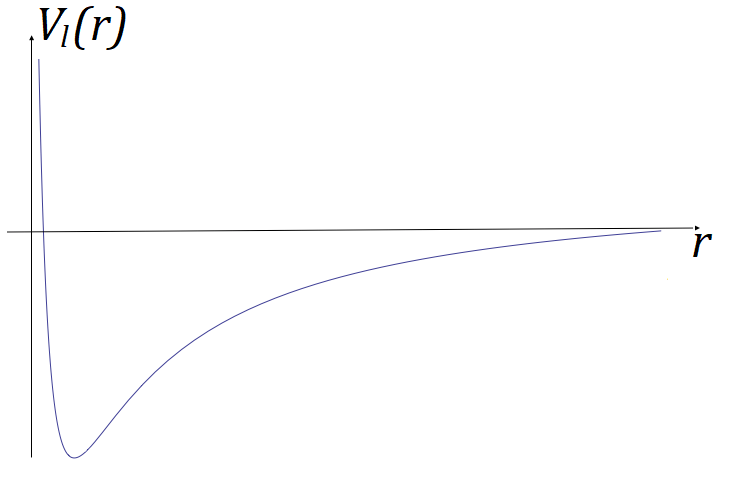
\includegraphics[width=8.5cm]{immagini/cap_21/fig_21_1.png}
\end{center}
\end{figure}\\
Si vede allora che lo spettro degli autovalori negativi dell'energia è discreto e corrisponde agli stati legati del sistema, mentre quello delle energie positive è continuo ed il moto corrispondente si estende da zero all'infinito.\\
Consideriamo qui in particolare il caso dello spettro discreto ossia degli stati legati degli atomi idrogenoidi.\\
L'equazione di Schr\"{o}dinger per le funzioni radiali si scrive:
\begin{equation}
\left[-\frac{\hbar^2}{2m}\frac{1}{r^2}\frac{d}{d r}\left(r^2\frac{d}{d r}\right)+\frac{\hbar^2l\left(l+1\right)}{2mr^2}\right]R\left(r\right)-\left(\frac{Ze^2}{r}+E\right)R\left(r\right)=0 .
\label{21.4}
\end{equation}

Per risolvere questa equazione risulta conveniente introdurre in primo luogo delle variabili adimensionali. Dalla precedente equazione risultano evidenti le seguenti uguaglianze "dimensionali"

\begin{equation}
\left[E\right]=\left[\frac{Ze^2}{r}\right]=\left[\frac{\hbar^2}{mr^2}\right] ,
\end{equation}

ossia

\begin{equation}
\left[r\right]=\left[\frac{\hbar^2}{mZe^2}\right] , \ \ \ \ ;\ \ \ \ \ \left[E\right]=\left[\frac{m\left(Ze^2\right)^2}{\hbar^2}\right] .
\end{equation}

Introduciamo allora, in luogo dell'energia, una nuova variabile definita da

\begin{equation}
E=-\frac{1}{2n^2}\frac{m\left(Ze^2\right)^2}{\hbar^2} .
\label{21.5}
\end{equation}
Per energie negative $n$ è un numero reale positivo.\\
In luogo del raggio $r$ introduciamo poi la variabile adimensionale $\rho$ definita da 
\begin{equation}
r=\frac{n}{2}\frac{\hbar^2}{mze^2}\rho .
\label{21.6}
\end{equation}
Sostituendovi le (\ref{21.5}) e (\ref{21.6}), l'equazione (\ref{21.4}) diventa:

\begin{eqnarray}
& & \frac{\hbar^2}{2m}\left(\frac{2mZe^2}{n\hbar^2}\right)\left[\frac{1}{\rho^2}\frac{d}{d\rho}\left(\rho^2\frac{d}{d\rho}\right)-\frac{l\left(l+1\right)}{\rho^2}\right]R +\nonumber \\
& & \qquad \qquad \quad +\left[\frac{2m\left(Ze^2\right)^2}{n\hbar^2}\frac{1}{\rho}-\frac{m\left(Ze^2\right)^2}{2n^2\hbar^2}\right]R=0 ,
\end{eqnarray}

ossia, dividendo per $2m\left(Ze^2\right)^2/\left(n^2\hbar^2\right)$ ed esplicitando le derivate:
\begin{equation}
\frac{d^2R}{d\rho^2}+\frac{2}{\rho}\frac{dR}{d\rho}+\left[-\frac{l\left(l+1\right)}{\rho^2}+\frac{n}{\rho}-\frac{1}{4}\right]R=0 .
\label{21.7}
\end{equation}

Consideriamo dapprima le soluzioni asintotiche dell'equazione (\ref{21.7}) valide per $\rho\rightarrow0$ (che è un punto singolare) e $\rho\rightarrow\infty$.\\
Nel limite $\rho\rightarrow0$ l'equazione (\ref{21.7}) si riduce a:

\begin{equation}
\frac{d^2R}{dR\rho^2}+\frac{2}{\rho}\frac{dR}{dR\rho}-\frac{l\left(l+1\right)}{\rho^2}R=0 .
\label{21.8}
\end{equation}

Cerchiamo una soluzione di questa equazione della forma
\begin{equation}
R\left(\rho\right)=\mbox{cost.} \rho^s .
\end{equation}

Sostituendo questa espressione nell'equazione (\ref{21.8}) si ottiene:

\begin{equation}
s\left(s-1\right)+2s-l\left(l+1\right)=0 ,
\end{equation}

ossia
\begin{equation}
s\left(s+1\right)=l\left(l+1\right) ,
\end{equation}

che ha come soluzione

\begin{equation}
s=\frac{-1\pm\sqrt{1+4l\left(l+1\right)}}{2}=\frac{-1\pm\left(2l+1\right)}{2}=\begin{cases}l\\-\left(l+1\right)\end{cases}
\end{equation}

La soluzione $s=-\left(l+1\right)$ deve essere scartata perché  conduce ad una f.d.o. divergente nell'origine, nell'intorno dell'origine di ha quindi

\begin{equation}
R\left(\rho\right)\simeq\rho^l , \ \ \ \ \ \ \ \ \left(\rho\rightarrow0\right) .
\end{equation}

Osserviamo che questo risultato rimane valido per ogni potenziale che nell'origine diverge più lentamente del potenziale centrifugo, ossia più lentamente di $1/r^2$. Il suo significato è che quanto più grande è il valore del momento angolare, tanto più piccolo è la probabilità di trovare la particella nell'origine.
Questo risultato è in accordo anche con le previsioni classiche.\\
Studiando ora l'equazione per grandi $\rho$, ossia nel limite $\rho\rightarrow\infty$. In tale approssimazione l'equazione (\ref{21.7}) si riduce a:
\begin{equation}
\frac{d^2R}{d\rho^2}-\frac{1}{4}R=0 .
\end{equation}
La cui soluzione è
\begin{equation}
R\left(\rho\right)=e^{\pm\rho/2} . 
\end{equation}
La soluzione che si annulla all'infinito, la sola fisicamente accettabile, è:
 
\begin{equation}
R\left(\rho\right)=e^{-\rho/2} .
\end{equation}
In definitiva concludiamo che la soluzione cercata è della forma
\begin{equation}
R\left(\rho\right)=\rho^le^{-\rho/2}w\left(\rho\right) ,
\label{21.9}
\end{equation}
dove $w$ è una funzione da determinare che deve divergere all'infinito non più rapidamente di una potenza finita di $\rho$ e deve essere finita per $\rho=0$.\\
Sostituendo la f.d.o. (\ref{21.9}) nell'equazione radiale (\ref{21.7}), e considerando che 
\begin{equation}
\frac{dR}{d\rho}=\rho^{l-1}e^{-\rho/2}[lw-\frac{1}{2}\rho w+\rho w^\prime] ,
\end{equation}
e
\begin{equation}
\frac{d^2R}{d\rho^2}=\rho^{l-2}e^{-\rho/2}\left[\rho^2w^{\prime\prime}+\left(2l-\rho\right)\rho w^\prime+\left(l\left(l-1\right)-l\rho+\frac{1}{4}\rho^2\right)w\right] ,
\end{equation}

otteniamo per w l'equazione
\begin{equation}
\rho w^{\prime\prime}+\left(2l+2-\rho\right)w^\prime+\left(n-l-1\right)w=0 .
\end{equation}
Cerchiamo per la soluzione $w\left(\rho\right)$ un'espressione per serie, poniamo cioè 

\begin{equation}
w\left(\rho\right)=\sum_{k=0}^\infty a_k \rho^k .
\end{equation}

Sostituendo nell'equazione di $w$ otteniamo:
\begin{equation}
\sum_{k=0}^\infty\left[a_{k+1}k\left(k+1\right)+\left(2l+2\right)\left(k+1\right)a_{k+1}-ka_k+\left(n-l-1\right)a_k\right]\rho^k=0 .
\end{equation}
Poiché la serie sia nulla per ogni valore di $\rho$ devono essere separatamente nulli i coefficienti di ogni potenza di $\rho$, si deve cioè avere
\begin{equation}
a_{k+1}=\frac{k-n+l+1}{\left(k+1\right)\left(k+2l+2\right)}a_k .
\end{equation}
L'andamento asintotico dei coefficienti della serie, per grandi valori di $k$, risulta tale che
\begin{equation}
\frac{a_{k+1}}{a_k}\simeq \frac{1}{k},
\end{equation}
pertanto
\begin{eqnarray}
a_{k+1}=\frac{a_{k+1}}{a_{k}}\frac{a_{k}}{a_{k-1}}\frac{a_{k-1}}{a_{k-2}}\dots \frac{a_{1}}{a_{0}}a_0 \simeq \nonumber \\
\simeq \frac{1}{k} \frac{1}{k-1}\frac{1}{k-2}\dots a_0\simeq \frac{a_0}{k!}  .
\end{eqnarray}
Ma in questo caso
\begin{equation}
w(\rho) =\sum _{k=0} ^{\infty} a_n\rho ^k \approx a_0 \sum _k \frac{\rho ^k}{k!} \approx a_0\ e^{\rho}.
\end{equation}
la funzione $w (\rho )$ così trovata non soddisfa la condizione al contorno all'infinito. Perché $w(\rho )$ diverga all'infinito come una potenza finita di $\rho$ deve essere $(n-l-1)$ un numero intero positivo o nullo. In tal caso al serie viene interrotta e $w (\rho )$ si riduce ad un polinomio di grado $(n-l-1)$. Siamo così giunti alla conclusione che \textbf{il numero $n$ deve essere un intero positivo e, per $l$ dato, si deve avere:}
\begin{equation}
n \geq l+1.
\end{equation}
Ricordando la definizione del parametro $n$ troviamo
\begin{equation}
E_n= -\frac{m\left(Ze^2\right) ^2}{2\hbar ^2 n^2}\qquad n=1,2,\dots
\end{equation}
Lo spettro discreto in un campo coulombiano è costituito dunque da un'infinità di livelli compresi tra il livello fondamentale
\begin{equation}
-\frac{m\left(Ze^2\right) ^2}{2\hbar ^2 }\simeq Z^2 \left(13.6 \textrm{eV}\right)
\end{equation}
e zero. Gli intervalli tra due livelli consecutivi diminuiscono al crescere di $n$. I livelli si infittiscono man mano che ci si avvicina al valore $E=0$, dove lo spettro discreto si connette con quello continuo.\\
Il numero intero $n$ è detto \textbf{numero quantico principale}. Per un numero quantico principale dato, il numero $l$ può assumere i valori
\begin{equation}
l=0,1,\dots,n-1,
\end{equation}
in totale $n$ valori diversi.\\
Nell'espressione dell'energia entra solo il numero $n$. pertanto tutti gli stati con $l$ diversi, ma con uguali $n$, hanno la stessa energia. Ogni autovalore è quindi degenere non soltanto rispetto al numero quantico $m$ (come per qualsiasi moto in un campo a simmetria centrale) ma anche rispetto al numero $l$. Quest'ultima \textbf{degenerazione}, detta \textbf{accidentale}, è specifica del campo coulombiano. Ad ogni valore di $l$ dato corrispondono $2l+1$ valori differenti di $m$. pertanto \textbf{l'ordine di degenerazione dell' n-esimo livello energetico è}, considerando anche la degenerazione di spin:
\begin{equation}
2 \left[ \sum _{l=0} ^{n-1} \left(2l+1 \right)\right]=2 \left[ 2\frac{\left( n-1 \right) n}{2}+n\right],
\end{equation}
ossia
\begin{equation}
2 \left[ \sum _{l=0} ^{n-1} \left(2l+1 \right)\right]= 2n^2.
\end{equation}
I polinomi che si ottengono interrompendo la serie che esprime $w(\rho)$ sono i cosiddetti \textbf{polinomi generalizzati di Laguerre.} Le f.d.o. radiali complete normalizzate con la condizione
\begin{equation}
\int _0 ^{\infty} dr r^2 {R_{nl} (r)}^2=1,
\end{equation}
hanno la forma
\begin{equation}
R_{nl}(r) =\frac{2}{n^2}\sqrt{\frac{\left(n-l-1\right) !}{\left(n+l\right) !}} e^{-\frac{\bar{r}}{n}}\left(\frac{2\bar{r}}{n}\right) ^l L_{n-l-1} ^{2l+1} \left(\frac{2\bar{r}}{n}\right) ,
\end{equation}
dove $L_k ^a (x)$ sono i polinomi generalizzati di Laguerre e
\begin{eqnarray}
\bar{r}= Z\frac{r}{a_0},\\
a_0= \frac{\hbar ^2}{me^2}.
\end{eqnarray}
la grandezza $a_0$ è detta \textbf{ragio di Bohr} e vale
\begin{equation}
a_0 \simeq 0.529 \times 10^{-8} \textrm{cm}.
\end{equation}
La decrescita esponenziale delle f.d.o. radiali indica che $n a_0/Z$ rappresenta la tipica dimensione radiale delle orbite stazionarie per un dato valore del numero quantico principale $n$. Inoltre le orbite sono tanto più vicine al nucleo quanto più è alta la carica elettrica $Z$ di quest'ultimo.\\
A partire dalla dimensione tipica del raggio delle orbite, $r \backsim a_0$, deriviamo la tipica \textbf{velocità del moto dell'elettrone}, utilizzando il principio di indeterminazione. Si ha:
\begin{eqnarray}
r & \backsim & a_0 =\frac{\hbar ^2}{me^2} \Rightarrow \nonumber \\
& \Rightarrow & v=\frac{p}{m} \backsim \frac{1}{m} \frac{\hbar}{r}\backsim \frac{\hbar}{m}\frac{me^2}{\hbar ^2}=\frac{e^2}{\hbar}, 
\end{eqnarray}
da cui
\begin{equation}
\frac{v}{c}\backsim \frac{e^2}{\hbar c}=\alpha \simeq \frac{1}{137}.
\end{equation}
\section{Modello di Bohr dell'atomo di idrogeno (1913)}
Tre ipotesi:
\begin{enumerate}
\item L'elettrone ruota attorno al nucleo su orbita stabile (senza emettere radiazione);
\item Le sole orbite consentite sono quelle per le quali il momento angolare risulta essere un multiplo intero di $\hbar$:
\begin{equation}
L=mvr=h\hbar;
\label{eq:21.10}
\end{equation}
\item L'elettrone può effettuare transizioni discontinue tra due orbite consentite. Quando ciò accade viene emessa o assorbita radiazione di frequenza
\begin{equation}
\hbar \omega = E-E'
\end{equation}
dove $\Delta E = E-E'$ è la variazione di energia dell'elettrone tra le due orbite.
\end{enumerate}
\textbf{Conseguenze:} la stabilità di un'orbita è determinata dall'equilibrio tra la forza coulombiana e la forza centrifuga:
\begin{eqnarray}
&\displaystyle{\frac{e^2}{r^2}=\frac{mv^2}{r}.}&\\
&\textrm{N.B. Forza centrifuga: } F=m\omega ^2 r = \frac{mv^2}{r}. \qquad \qquad (v=\omega r)& \nonumber
\end{eqnarray}
Questa condizione, unita alla (\ref{eq:21.10}), fornisce
\begin{equation}
\begin{cases}
mv^2r=e^2\\
mvr=n\hbar
\end{cases}
\Rightarrow \ v=\frac{e^2}{n\hbar}, \quad r=\frac{n\hbar}{mv}=\frac{n^2\hbar ^2}{me^2},
\end{equation}
dunque
\begin{eqnarray}
&r=n^2\frac{\hbar^2}{me^2}=n^2a_0, \qquad \left[\textrm{In meccanica quantistica } \langle \frac{1}{r}\rangle =\frac{1}{n^2 a_0}\right]& \\
&\frac{v}{c}=\frac{1}{n}\frac{e^2}{\hbar c}=\frac{\alpha}{n}. \qquad \qquad \left[\textrm{In meccanica quantistica } \langle \frac{v^2}{c^2}\rangle =\frac{\alpha ^2}{n^2}\right]&
\end{eqnarray}
Calcoliamo l'energia delle orbite:
\begin{eqnarray}
&\displaystyle{\frac{p^2}{2m}=\frac{mv^2}{2}=\frac{me^4}{2n^2\hbar ^2}=\frac{mc^2 \alpha ^2}{2n^2}} ,& \\
\nonumber \\
&\displaystyle{\frac{e^2}{r}=\frac{me^4}{n^2\hbar ^2}=\frac{mc^2 \alpha ^2}{n^2}} ,&\\
& \left[\textrm{N.B. In M.Q. valgono questi stessi risultati per i valori medi di T e V.}\right]& \nonumber
\end{eqnarray}
da cui
\begin{equation}
E=\frac{p^2}{2m}-\frac{e^2}{r}=-\frac{mc^2\alpha ^2}{2n^2}.
\end{equation}
Le righe di emissione e assorbimento dell'atomo hanno pertanto frequenze della forma
\begin{equation}
\hbar \omega =E-E' = \frac{mc^2\alpha ^2}{2} \left( \frac{1}{n'^2}-\frac{1}{n^2}\right).
\end{equation}
\section{Trucchi con le costanti fondamentali}
In luogo di $c$, $\hbar$, $e$, $m_e$ utilizzare:
\begin{itemize}
\item $\displaystyle{\alpha =\frac{e^2}{\hbar c}}= \frac{1}{137}$, costante di struttura fine;
\item $\displaystyle{r_0 =\frac{e^2}{m_e c^2}=2.82 \times 10^{-13}}$ cm ($=2.82$ fm), raggio classico dell'elettrone;
\item $\displaystyle{m_ec^2=0.511}$ MeV, massa a riposo dell'elettrone;
\item $\displaystyle{c=3\times 10^{10}}$ cm/s, velocità della luce nel vuoto.
\end{itemize}
Esempi:
\begin{itemize}
\item[ ]Raggio di Bohr:
\begin{eqnarray}
a_o &=&\frac{\hbar ^2}{me^2}=\left( \frac{\hbar c}{e^2}\right)\frac{e ^2}{mc^2}=\frac{r_0}{\alpha ^2} \nonumber \\
&\simeq &(137)^2\cdot 2.82 \cdot 10^{-13}=0.529\cdot10^{-10} \textrm{ cm}\ (=0.529 \textrm{ Å})\nonumber
\end{eqnarray}
\item[ ]Lunghezza d'onda Compton dell'elettrone:
\begin{eqnarray}
\lambda _e &=&\frac{\hbar}{mc}=\frac{\hbar}{e^2}\frac{e^2}{mc}= \frac{r_0}{\alpha}= \nonumber \\
&\simeq & 137\cdot 2.82\cdot 10^{-13} \textrm{ cm}= 3.86 \cdot 10^{-11} \textrm{ cm} \nonumber
\end{eqnarray}
\item[ ]Livelli di energia dell'atomo di idrogeno:
\begin{eqnarray}
E_n &=& -\frac{me^4}{2n^2\hbar^2}=-\frac{1}{2n^2}mc^2 \left(\frac{e^2}{\hbar c^2}\right)^2= -\frac{mc^2 \alpha ^2}{2n^2}= \nonumber \\
&\simeq & -\frac{1}{n^2}\frac{0.511 \textrm{ MeV}}{2\cdot (137)^2}=-\frac{1}{n^2}13.6 \textrm{ eV}. \nonumber
\end{eqnarray}
\item[ ]Costante di Planck:
\begin{eqnarray}
\hbar =\frac{\hbar c}{e^2}\frac{e^2}{mc^2}\frac{mc^2}{c}=\frac{1}{\alpha}\frac{r_0 mc^2}{c}\simeq 6.58\cdot10^{-22} \textrm{ MeV}\cdot \textrm{s} \nonumber 
\end{eqnarray}
\end{itemize}
\section[Raggio classico dell'elettrone]{Raggio classico dell'elettrone: significato fisico}
Schematizziamo l'elettrone come una sfera di raggio $a$ sulla cui superficie è distribuita una carica $e$.\\
Il campo elettrico generato dalla carica è:
\begin{equation}
E=\begin{cases}
0 \qquad \textrm{per }r<a;\\
\\
\displaystyle{\frac{e}{r^2}} \qquad \textrm{per }r>a.
\end{cases}
\end{equation}
La densità associata al campo è:
\begin{equation}
U=\frac{E^2}{8\pi}=\begin{cases}
0 \qquad \textrm{per }r<a;\\
\\
\displaystyle{\frac{e^2}{8\pi r^4}} \qquad \textrm{per }r>a.
\end{cases}
\end{equation}
L'energia totale è dunque
\begin{equation}
E_{el}=\int U dV = \int _a ^{\infty} \frac{e^2}{8\pi r^4} 4\pi r^2 dr = \frac{e^2}{2} \int _a ^{\infty} \frac{dr}{r^2}=\frac{e^2}{2a}. 
\end{equation}
Uguagliando questa energia all'energia di riposo dell'elettrone, $E=m_e c^2$, ricaviamo il raggio dell'elettrone:
\begin{equation}
a=\frac{1}{2}\frac{e^2}{mc^2}=\frac{1}{2} r_0,
\end{equation}
dove $r_0$ è il raggio classico dell'elettrone. il fattore $\frac{1}{2}$, ottenuto nella precedente espressione, è una conseguenza dei dettagli del modello e segue in particolare dall'aver scelto la carica distribuita solo sulla superficie della sfera (e non, ad esempio, all'interno della sfera stessa). notiamo anche che l'energia associata ad una carica puntiforme ($a=0$) risulta infinita.
\begin{figure}[!htbp]
\begin{center}
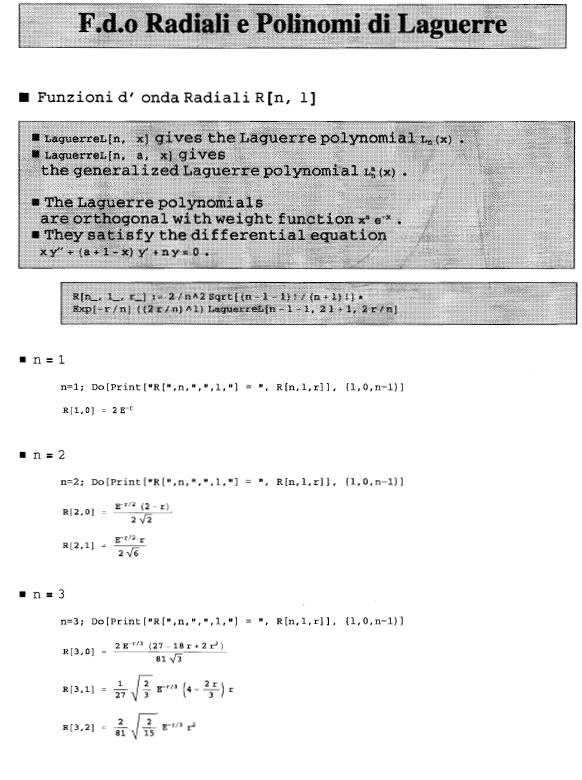
\includegraphics[width= \textwidth]{immagini/cap_21/fig_21_2.png}\\
\end{center}
\end{figure}
\begin{figure}[!htbp]
\begin{center}
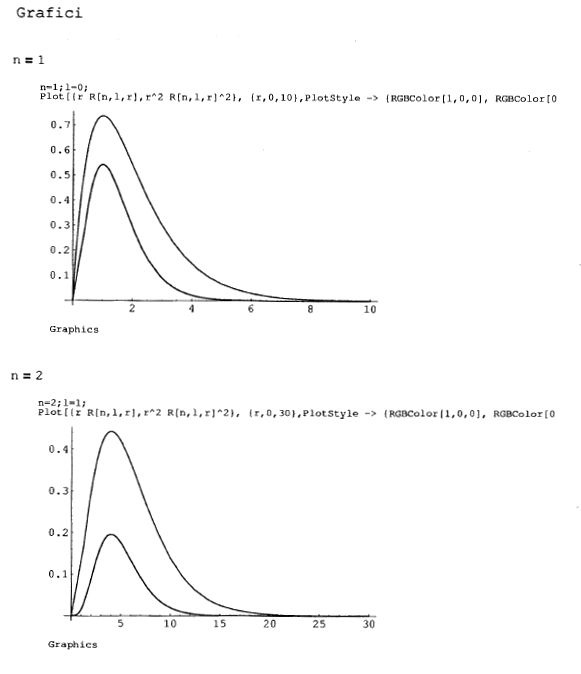
\includegraphics[width= \textwidth]{immagini/cap_21/fig_21_3.png}\\
\end{center}
\end{figure}
\begin{figure}[!htbp]
\begin{center}
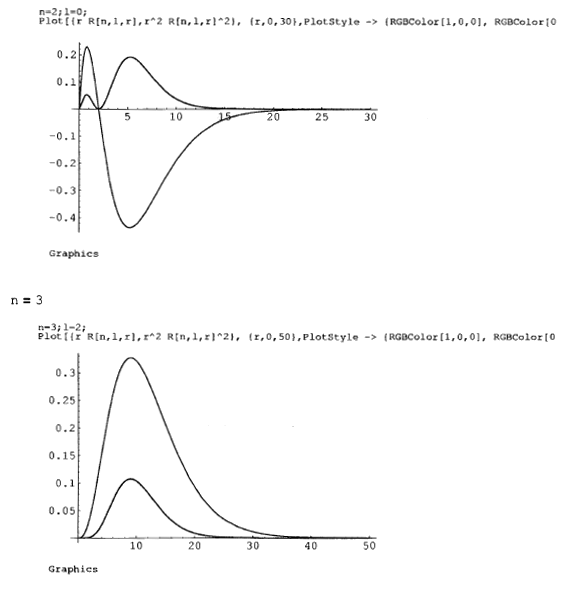
\includegraphics[width= \textwidth]{immagini/cap_21/fig_21_4.png}\\
\end{center}
\end{figure}
\begin{figure}[!htbp]
\begin{center}
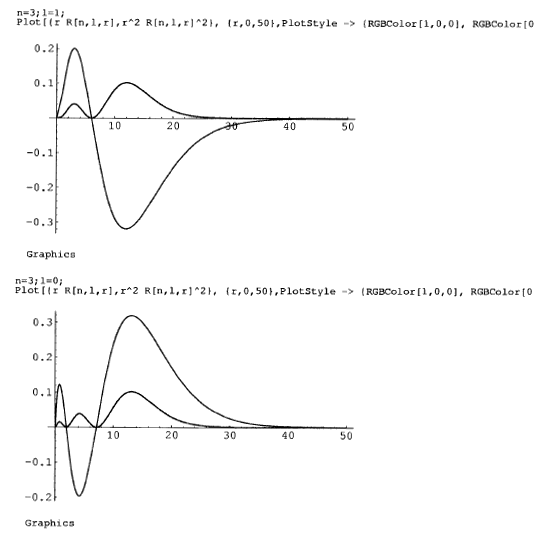
\includegraphics[width= \textwidth]{immagini/cap_21/fig_21_5.png}
\end{center}
\end{figure}%DEFINITIVO
\chapter[Particella in campo elettromagnetico]{Hamiltoniana di una particella in un campo elettromagnetico esterno}
Nella \textbf{teoria classica} l'hamiltoniana di una particella di carica elettrica e (e<0 per l'elettrone) ha la forma:
\begin{equation}
H=\frac{1}{2m}(\vec{p}-\frac{e}{c}\vec{A}\;)^{2}+e\Phi ,
\label{22.1}
\end{equation}
dove $\Phi$ è il potenziale scalare ed $\vec{A}$ è il potenziale vettoriale del campo, $\vec{p}$ la quantità di moto generalizzata della particella.
L'espressione (\ref{22.1}) per l'hamiltoniana può essere ottenuta, a partire dall'hamiltoniana H=$\vec{p}^{\;2}/2m$ per la particella libera, effettuando la \textbf{sostituzione minimale}:
\begin{equation}
E\rightarrow E-e\Phi,\; \vec{p}\rightarrow \vec{p}-\frac{e}{c}\vec{A} .
\end{equation}
\textbf{Se la particella non ha spin il passaggio alla meccanica quantistica avviene nel modo solito: la quantità di moto generalizzata $\vec{p}$ va sostituita con l'operatore:}
\begin{equation}
\vec{p}=-i\hbar \vec{\nabla} .
\end{equation}
Sviluppando il quadrato ($\vec{p}-\frac{e}{c}\vec{A}$)$^{2}$ occorre tener presente che l'operatore $\vec{p}$ non commuta in generale, con il vettore $\vec{A}$ che è funzione delle coordinate. Si deve quindi scrivere:
\begin{equation}
H= \frac{\vec{p}^{\;2}}{2m}-\frac{e}{2mc}(\vec{p}\cdot\vec{A}+\vec{A}\cdot\vec{p}\;)+\frac{e^{2}}{2mc^{2}}\vec{A}^{\;2}+e\Phi .
\label{22.4}
\end{equation}
Calcoliamo il commutatore tra $\vec{p}$ ed $\vec{A}$. Si ha:
\begin{eqnarray}
\vec{p}\cdot\vec{A}&=&-i\hbar \vec{\nabla}\cdot\vec{A}=-i\hbar\partial_{j}A_{j}= \nonumber \\
&=&-i\hbar(\partial_{j}A_{j})-i\hbar A_{j}\partial_{j}= \nonumber \\
&=& -i\hbar(\vec{\nabla}\cdot\vec{A})-i\hbar\vec{A}\cdot\vec{\nabla} ,
\end{eqnarray}
ossia $\vec{p}\cdot\vec{A}-\vec{A}\cdot\vec{p}=-i\hbar\vec{\nabla}\cdot\vec{A}$.\\ Così \textbf{$\vec{p}$ ed $\vec{A}$ commutano se $\vec{\nabla}\cdot\vec{A}$ è uguale a zero}.\\ La divergenza di $\vec{A}$ si annulla, in particolare, per un \textbf{campo omogeneo} se definiamo il suo potenziale vettore nel modo seguente:
\begin{equation}
\vec{A}=\frac{1}{2}\vec{B}\wedge\vec{r} .
\label{22.6}
\end{equation}
Questa definizione è consistente giacché conduce a:
\begin{eqnarray}
(\vec{\nabla}\times\vec{A})_{i}&=&\varepsilon_{ijk}\partial_{j}A_{k}=\frac{1}{2}\varepsilon_{ijk}\varepsilon_{klm}\partial_{j}B_{l}r_{m}= \nonumber \\
&\overset{\partial_{j}B_{l}=0}{=}&  \frac{1}{2}\varepsilon_{ijk}\varepsilon_{klm}B_{l}=\frac{1}{2}\varepsilon_{ijk}\varepsilon_{ljk}B_{l}=B_{i} ,
\end{eqnarray}
ossia $\vec{B}=\vec{\nabla}\wedge\vec{A}$.\\
Inoltre calcolando la divergenza del potenziale vettore definito dall'equazione (\ref{22.6}) otteniamo:
\begin{equation}
\vec{\nabla}\cdot\vec{A}=\partial_{i}A_{i}=\frac{1}{2}\varepsilon_{ijk}\partial_{i}B_{j}r_{k}=0 ,
\end{equation}
ossia $\vec{\nabla}\cdot\vec{A}=0$\\
Sostituendo il potenziale vettore $\vec{A}$ dato dalla (\ref{22.6})nell'espressione (\ref{22.4})dell'hamiltoniana, ed osservando che vale la relazione
\begin{equation}
\vec{A}\cdot\vec{p}=\frac{1}{2}\varepsilon_{ijk}B_{j}r_{k}p_{i}=\frac{1}{2}\vec{B}\cdot(\vec{r}\wedge\vec{p}\;)=\frac{1}{2}\vec{B}\cdot\vec{L} ,
\end{equation}
dove $\vec{L}$ è il momento angolare orbitale della particella, otteniamo:
\begin{equation}
H=\frac{\vec{p}^{\;2}}{2m}-\frac{e}{2mc}\vec{L}\cdot\vec{B}+\frac{e^{2}}{8mc^{2}}(\vec{B}\wedge\vec{r}\;)+e\Phi .
\label{22.10}
\end{equation}
Nella fisica atomica il termine quadratico nel campo magnetico esterno $\vec{B}$ risulta tipicamente trascurabile rispetto al termine lineare nel campo.\\
Quanto al termine lineare nel campo, questo mostra che \textbf{una particella carica priva di spin, in moto in un campo magnetico esterno, possiede un momento magnetico $\vec{\mu}$, proporzionale al suo momento angolare orbitale, dato da}:
\begin{equation}
\vec{\mu}=\frac{e}{2mc}\vec{L} .
\label{22.11}
\end{equation} 
Il rapporto tra il momento magnetico $\vec{\mu}$ e il momento angolare orbitale $\vec{L}$ è pari ad $e/2mc$, risultato identico a quello che si ottiene in meccanica classica. Per l'elettrone il valore di questo rapporto, moltiplicato per la costante di Planck $\hbar$, definisce una grandezza chiamata \textbf{magnetone di Bohr}.
\begin{equation}
\mu_{B}=\frac{|e|\hbar}{2m_{e}c}=0.927\cdot10^{-20}\frac{erg}{gauss} .
\end{equation}
La teoria sin qui considerata resta tuttavia incompleta se non si tiene conto del fatto che le particelle possiedono, in generale, oltre ad un momento angolare orbitale, anche un momento angolare intrinseco, lo \textbf{spin}. È dimostrato sperimentalmente che, in conseguenza di ciò, gli elettroni, ad esempio, possiedono anche un \textbf{momento magnetico intrinseco}, legato allo spin $\vec{S}$ dalla relazione:
\begin{equation}
\vec{\mu}=\frac{|e|}{m_{e}c}\vec{S} .
\label{22.13}
\end{equation}
Tale risultato trova una spiegazione solo nell'ambito della \textbf{teoria relativistica}. Si osservi in particolare come questa relazione differisca dall'analoga relazione (\ref{22.11}) per il \textbf{fattore 2} al denominatore.\\
Il coefficiente di proporzionalità tra il momento magnetico intrinseco e lo spin di una particella varia, in generale, da particella a particella. Per il protone, ad esempio, questo coefficiente vale circa 2.79($e/m_{p}c$), dove $m_{p}$ è la massa del protone, mentre per il neutrone vale -1.91($e/m_{p}c$).\\
L'esistenza di un momento magnetico intrinseco, per le particelle dotate di spin, richiede l'aggiunta all'hamiltoniano (\ref{22.10}), di un termine che descrive \textbf{l'interazione della particella con il campo magnetico esterno}. Per l'elettrone, tale termine è dato, in accordo con l'equazione(\ref{22.13}), da:
\begin{equation}
H=-\vec{\mu}\cdot\vec{B}=\frac{|e|}{m_{e}c}\vec{S}\cdot\vec{B} .
\end{equation}
L'hamiltoniano completo che descrive l'elettrone in un campo elettromagnetico esterno omogeneo ha dunque la forma:
\begin{equation}
H=\frac{\vec{p^{\;2}}}{2m}+\frac{|e|}{2m_{e}c}(\vec{L}+2\vec{S})+\frac{e^{2}}{8m_{e}c}(\vec{B}\wedge\vec{r}\;)^{2}-|e|\Phi .
\end{equation}%DEFINITIVO
\chapter[Effetto Stark]{Effetto Stark\footnote{G16; S5.1,5.2}}
Se un atomo viene sottoposto ad un campo elettrico esterno, i suoi livelli energetici cambiano. Questo fenomeno è detto \textbf{effetto Stark}.
Supporremo che il campo elettrico sia sufficientemente debole, perché l'energia addizionale ad esso dovuta sia piccola rispetto alle distanze fra i livelli energetici vicini dell'atomo. Allora per calcolare gli spostamenti dei livelli un un campo elettrico, si può ricorrere alla \textbf{teoria delle perturbazioni}.\\
Ci proponiamo di calcolare, facendo uso della teoria delle perturbazioni, le correzioni al primo ordine da apportare ai livelli energetici dell'\textbf{atomo di idrogeno}.\\
Scegliendo la direzione ed il verso dell'asse $z$ parallelo al campo elettrico $\mathcal{E}$ possiamo scrivere l'hamiltoniano del sistema perturbato come
\begin{equation}
H=H_0+V, 
\end{equation}
dove
\begin{equation}
H_0=\frac{p^2}{2m}-\frac{\mathcal{Z}e^2}{r},
\end{equation}
($\mathcal{Z}=1$ per l'atomo di idrogeno) è l'hamiltoniano imperturbato e
\begin{equation}
V=+e\mathcal{E}z
\end{equation}
è la perturbazione introdotta.\\
In assenza della perturbazione lo stato dell'elettrone nell'atomo di idrogeno è, negli stati stazionari, individuato da tre numeri quantici $n,l,m$. Indichiamo tali stati con $\boldsymbol{|n,l,m\rangle}$.
Consideriamo inizialmente la \textbf{correzione} da apportare \textbf{al livello energetico dello stato fondamentale}. Tale stato non è degenere e possiamo allora scrivere
\begin{equation}
E^{(1)}_{100}=V_{11}=\langle100| V |100\rangle =+e\mathcal{E}\langle 100 | z |100 \rangle,
\end{equation}
Questa correzione è nella. Essa può essere infatti scritta in termini di un integrale della forma
\begin{equation}
E^{(1)}_{100}=e\mathcal{E} \int d^3r \left|\phi_{100}(\vec{r})\right|^2 z=0,
\end{equation}
che è nullo in virtù della simmetria sferica della funzione d'onda nella stato fondamentale. \textbf{In prima approssimazione, allora, il campo elettrico non altera il livello energetico fondamentale}.\\
\textbf{La correzione} al livello energetico dello stato fondamentale \textbf{risulta non nulla al secondo ordine della teoria delle perturbazioni}. Questa correzione è espressa dalla sommatoria
\begin{equation}
\label{eq:cap23_1}
E^{(2)}_{100}=e^2 \mathcal{E}^2 \sum_{k\neq(100)}\frac{\left| \langle k^{(0)} | z |100 \rangle \right|^2}{E^{(0)}_{100}-E^{(0)}_{k}},
\end{equation}
estesa non solo agli stati legati $|n,l,m \rangle$ (con $n>1$) ma anche agli stati del continuo con energia positiva dell'atomo di idrogeno.\\
La sommatoria che compare nell'espressione ($\ref{eq:cap23_1}$) può essere calcolata esattamente e si trova:
\begin{equation}
E^{(2)}_{100}=-\frac{9}{4} \mathcal{E}^2 \left( \frac{a_0}{z} \right)^3,
\end{equation}
dove $a_0$ è il raggio di Bohr. (Osserviamo che $\int d^3r \mathcal{E}^2$ è un'energia, cosicché un'analisi dimensionale implica che comunque $E^{(2)}_{100}\sim\mathcal{E}^2\left( a_0/z \right)^3 $.\\
Poiché lo spostamento del livello energetico fondamentale dell'atomo di idrogeno risulta proporzionale al quadrato del campo elettrico esterno, tale effetto viene indicato con il nome di \textbf{effetto Stark quadratico}.\\
Consideriamo ora l'\textbf{effetto del campo elettrico sugli stati corrispondenti al primo livello eccitato dell'atomo di idrogeno ($\boldsymbol{n=2}$)}.\\
In questo caso, come si sa, il livello energetico è \textbf{quattro volte degenere}. I possibili valori dei numeri quantici sono: \\ \\
\begin{center}
$\begin{matrix} 
& &  &  &  & & \\
  & &  &  &  & m=1 & \cdot  \\
 &  &  &  & \iddots & &  \\
 &  &  & l=1 & \cdots & m=0 & \cdot \\
 &  & \iddots &  & \ddots & & \\
&  n=2 &  &  &  & m=-1 & \cdot \\
 &  & \ddots  & &  &  & \\
 &   &  & l=0 & \cdots & m=0 & \cdot \\
 & &  &  &  & & 
 \end{matrix}$ 
\end{center} 
\vspace{1cm}
Gli spostamenti del livello energetico sono allora determinati, in accordo con le formule della teoria delle perturbazioni nel caso degenere, dagli autovalori della matrice della perturbazione $V$ nel sottospazio degli autostati imperturbati degeneri. \\ Ordiniamo gli elementi di questa matrice secondo il seguente schema:
\begin{equation}  
V=
\bordermatrix{~&200&210&211&21-1\cr
& \cdot & \cdot & \cdot & \cdot \cr
& \cdot & \cdot & \cdot & \cdot \cr
& \cdot & \cdot & \cdot & \cdot \cr
& \cdot & \cdot & \cdot & \cdot \cr}
\end{equation}
Osserviamo, innanzitutto, che \textbf{l'operatore $\boldsymbol{V=e\mathcal{E}z}$ è invariante per rotazioni attorno all'asse $\boldsymbol{z}$}, ossia \textbf{la perturbazione commuta con l'operatore proiezione sull'asse $\boldsymbol{z}$ del momento angolare, $\boldsymbol{L_z=xp_y-yp_x}$}:
\begin{equation} 
\left[V,L_z\right]=0.
\end{equation}
Ne segue che \textbf{gli elementi della matrice $\boldsymbol{V}$ tra stati con diverso valore di $\boldsymbol{m}$ sono nulli}. Infatti 
\begin{eqnarray} 
0 & = & \langle n,l,m| \left[V,L_z\right] |n,l',m'\rangle= \nonumber \\
 & = &\langle n,l,m | \left(VL_z-L_zV\right)|n,l',m'\rangle= \nonumber \\
 & = &\left( m-m' \right) \langle n,l,m |V |n,l',m'\rangle
\end{eqnarray}
da cui
\begin{equation}
\langle n,l,m | V |n,l',m'\rangle=0 \qquad per \quad m \neq m'.
\end{equation}
Nel sottospazio degli stati degeneri corrispondenti ad $n=2$ la matrice $V$ ha allora la forma
\begin{equation} 
V=
\bordermatrix{~&200&210&211&21-1\cr
& \cdot & \cdot^{*} & 0 & 0 \cr
& \cdot^{*} & \cdot & 0 & 0 \cr
& 0 & 0 & \cdot & 0 \cr
& 0 & 0 & 0 & \cdot \cr}
\end{equation}
(gli elementi di matrice $*$ hanno lo stesso $m$).
È semplice dimostrare, inoltre, che \textbf{la perturbazione $\boldsymbol{V}$ anticommuta con l'operatore di parità}. Utilizzando per gli operatori la loro espressione nella rappresentazione delle coordinate, si ha infatti:
\begin{equation}
PV\phi(\vec{r})=e\mathcal{E}Pz\phi(\vec{r})=-e\mathcal{E}z\phi(\vec{-r})=-VP\phi(\vec{r}),
\end{equation}
ossia:
\begin{equation} 
\{P,V\}=0.
\end{equation}
Ne segue che \textbf{gli elementi di matrice della perturbazione tra stati con uguale parità sono nulli}. Considerando infatti due stati con parità $p_1$ e $p_2$ si ha:
\begin{eqnarray}
0 & = &\langle p_1 | \{ P,V \} |p_2\rangle= \langle p_1 | \left( PV+VP \right) |p_2 \rangle = \nonumber \\
 & =& (p_1+p_2)\langle p_1|V|p_2\rangle 
\end{eqnarray}
da cui 
\begin{equation} \label{eq:cap23_2}
\langle p_1| V |p_2\rangle=0 \qquad per \quad p_1=p_2.
\end{equation}
Discutiamo allora le \textbf{proprietà di simmetria degli autostati $\boldsymbol{|n,l,m \rangle}$ sotto operazione di parità}.\\
Cominciamo con l'osservare che l'operatore di parità $P$ commuta con l'operatore momento angolare orbitale $\vec{L}$ :
\begin{equation}
[ P, \vec{L} ]=0.
\end{equation}
Infatti $\vec{L}=\vec{r}\wedge \vec{p}$ e sia $\vec{r}$ sia $\vec{p}$ sono dispari per parità. Così:
\begin{eqnarray}
P\vec{L}\phi(\vec{r)} & = & P(\vec{r}\wedge\vec{p})\phi(\vec{r})= (\vec{-r}) \wedge (\vec{-p})\phi(\vec{-r})= \nonumber \\
& = & (\vec{r} \wedge \vec{p})\phi(\vec{-r})=\vec{L}P\phi(\vec{r}).
\end{eqnarray}
Ne segue anche che l'operatore di parità commuta con il quadrato del momento angolare orbitale
\begin{equation}
\left[ P,L^2\right]=0.
\end{equation}
Allora gli autostati di $L^2$ ed $L_z$ sono anche autostati dell'operatore di parità e si deve avere
\begin{equation}
P|l,m\rangle=\lambda_{l,m}|l,m\rangle.
\end{equation}
Inoltre, in virtù della commutatività tra l'operatore di parità e gli operatori a scala $L_{\pm}$, gli stati con stesso valore di $l$ e diverso valore di $m$ devono avere stessa parità. Infatti
\begin{eqnarray} 
 PL_-|l,m\rangle &= & cP|l,m-1\rangle=c\lambda_{l,m-1}|l,m-1\rangle=  \nonumber \\
&= & L_-P|l,m\rangle=L_- \lambda_{l,m}|l,m\rangle=c\lambda_{l,m}|l,m-1\rangle ,
\end{eqnarray}
ossia
\begin{equation} 
\lambda_{l,m}=\lambda_{l,m-1},
\end{equation}
e possiamo scrivere allora:
\begin{equation} 
P|l,m\rangle=\lambda_l|l,m \rangle.
\end{equation}
Per determinare la parità $\lambda_l$ osserviamo che una trasformazione di parità in coordinate polari è realizzata dalla trasformazione 

\begin{center}
\begin{minipage}[c]{0.35\textwidth}
\centering
\begin{equation}
\begin{cases} \nonumber
r \to r \\
\theta \to \pi-\theta \\
\varphi \to \varphi-\pi
\end{cases}
\end{equation}
\end{minipage}
\begin{minipage}{0.50\textwidth}
\centering
\tdplotsetmaincoords{60}{110}
%
\pgfmathsetmacro{\rvec}{.8}
\pgfmathsetmacro{\thetavec}{30}
\pgfmathsetmacro{\phivec}{60}
%
\begin{tikzpicture}[scale=5,tdplot_main_coords]
    \coordinate (O) at (0,0,0);
    \draw[thick,->] (0,0,0) -- (1,0,0) node[anchor=north east]{$x$};
    \draw[thick,->] (0,0,0) -- (0,1,0) node[anchor=north west]{$y$};
    \draw[thick,->] (0,0,0) -- (0,0,1) node[anchor=south]{$z$};
    \tdplotsetcoord{P}{\rvec}{\thetavec}{\phivec}
    \draw[-stealth,color=red] (O) -- (P) node[above right] {$\vec{r}$};
    \draw[dashed, color=red] (O) -- (Pxy);
    \draw[dashed, color=red] (P) -- (Pxy);
    \tdplotdrawarc{(O)}{0.2}{0}{\phivec}{anchor=north}{$\varphi$}
    \tdplotsetthetaplanecoords{\phivec}
    \tdplotdrawarc[tdplot_rotated_coords]{(0,0,0)}{0.5}{0}%
        {\thetavec}{anchor=south west}{$\theta$}
\end{tikzpicture}
\end{minipage}
\end{center}
L'effetto di una trasformazione di parità è facilmente calcolabile sugli stati con $m=l$, giacché in questo caso le corrispondenti autofunzioni hanno una forma particolarmente semplice:
\begin{equation} 
Y_{l,l}(\theta, \varphi)=A_l \left( \sin \theta \right)^l e^{il\varphi}.
\end{equation}
Si ha allora:
\begin{eqnarray} 
PY_{l,l}(\theta, \varphi) & = & A_l \left( \sin (\pi -\theta) \right)^l e^{il(\varphi+\pi)}= \nonumber \\
 & =  &A_l \left( \sin \theta \right)^l e^{il\varphi} e^{i \pi l}= (-1)^l Y_{l,l}(\theta, \varphi),
\end{eqnarray}
da cui, in definitiva:
\begin{equation} 
P|l,m\rangle= (-1)^l |l,m \rangle.
\end{equation}
Ricordando che la relazione ($\ref{eq:cap23_2}$), siamo portati a concludere che \textbf{gli elementi di matrice della perturbazione $\boldsymbol{V}$ tra due stati per i quali $\boldsymbol{l}$ è sempre pari o sempre dispari sono nulli}.\\
Siamo dunque giunti, per la matrice $V$, alla seguente espressione:
\begin{equation}  
V=
\bordermatrix{~&200&210&211&21-1\cr
& 0 & \cdot & 0 & 0 \cr
& \cdot & 0 & 0 & 0 \cr
& 0 & 0 & 0 & 0 \cr
& 0 & 0 & 0 & 0 \cr}
\end{equation}
Poiché la matrice è hermitiana, ci resta solo da calcolare l'elemento 
\begin{eqnarray} \label{eq:cap23_3}
\langle 210| V |200 \rangle & =&  \langle 200| V |210 \rangle^* = \nonumber \\
& = &\int d\Omega \ r^2 dr \ \phi_{210}^*(\vec{r}) V \phi_{200}(\vec{r}),
\end{eqnarray}
dove le funzioni d'onda rilevanti sono date dalle espressioni
\begin{eqnarray} 
\phi_{210}& = &R_{21}(r)Y_{10}(\theta, \varphi)= \nonumber  \\
& = & \frac{1}{\sqrt{3}}\left( \frac{1}{2a_0} \right)^{3/2} \left( \frac{r}{a_0} \right) e^{-\frac{r}{2a_0}} \sqrt{\frac{3}{4 \pi}} \cos \theta ,
\end{eqnarray}
\begin{eqnarray}
\phi_{200}& = & R_{20}(r)Y_{00}(\theta, \varphi)= \nonumber \\
& = & 2\left( \frac{1}{2a_0} \right)^{3/2} \left( 1-\frac{r}{2a_0} \right) e^{-\frac{r}{2a_0}} \sqrt{\frac{1}{4 \pi}} 
\end{eqnarray}
(Per gli atomo idrogenoidi si deve sostituire $a_0 \to \frac{a_0}{\mathcal{Z}}$)
Esprimiamo il potenziale $V$ in coordinate sferiche 
\begin{equation}
V=e \mathcal{E}z=e \mathcal{E} r \cos\theta
\end{equation}
e calcoliamo l'integrale ($\ref{eq:cap23_3}$) 
\begin{eqnarray}
 &  &\int r^2 dr d\Omega \   e \mathcal{E} r \cos\theta \cdot    \frac{2}{\sqrt{3}} \left( \frac{1}{2a_0} \right)^{3}   \left( \frac{r}{a_0} \right)     \left( 1-\frac{r}{2a_0} \right)  e^{-\frac{r}{a_0}} \cdot  \nonumber \\
 &  &\quad \  \cdot \sqrt{\frac{3}{4 \pi}} \cos \theta \sqrt{\frac{1}{4 \pi}}=  \nonumber \\ \nonumber
 & =& e \mathcal{E} \cdot \frac{2}{3}  \left( \frac{1}{2a_0} \right)^{3} \int_0^{\infty} dr \ r^3 \left( \frac{r}{a_0} \right)     \left( 1-\frac{r}{2a_0} \right)  e^{-\frac{r}{a_0}} \cdot \\ \nonumber
 & &\quad \ \cdot \int d\Omega \left| Y_{10}(\theta, \varphi) \right|^2=  \nonumber \\
 & =& e \mathcal{E} \cdot \frac{a_0}{12} \int_0^{\infty} ds \ s^4 \left(1-\frac{1}{2}s \right) e^{-s} = \nonumber \\
 & =& \frac{1}{12} \cdot e \mathcal{E} \cdot a_0 \left( 4!-\frac{1}{2}5! \right)= \frac{1}{12} \cdot  e \mathcal{E} \cdot a_0 (24-60),
\end{eqnarray}
ossia 
\begin{equation} 
\langle 210|V|200\rangle= \langle 200 |V |210 \rangle^*=-3e\mathcal{E}a_0. 
\end{equation}
\textbf{La matrice della perturbazione $\boldsymbol{V}$ nel sottospazio degli autostati degeneri corrispondenti agli stati con $\boldsymbol{n=2}$ ha dunque la forma}:
\begin{equation}  
V=
\bordermatrix{~&200&210&211&21-1\cr
& 0 & -3e\mathcal{E}a_0 & 0 & 0 \cr
& -3e\mathcal{E}a_0 & 0 & 0 & 0 \cr
& 0 & 0 & 0 & 0 \cr
& 0 & 0 & 0 & 0 \cr}
\end{equation}
Gli autovalori di questa matrice rappresentano le correzioni, al primo ordine nella perturbazione, ai livelli energetici imperturbati corrispondenti agli stati con $n=2$. Questi \textbf{autovalori} sono:
\begin{equation} 
E^{(1)}=0, \ \pm 3e\mathcal{E}a_0,
\end{equation}
con l'autovalore nullo avente molteplicità di 2. (Si osservi come la sottomatrice $2\times2$ da diagonalizzare è proporzionale alla matrice di Pauli $\sigma_1$).\\
Gli \textbf{autostati} corrispondenti agli autovalori $E^{(1)}=\pm 3e\mathcal{E}a_0$, nel sottospazio di dimensione  di interesse, sono dati da
\begin{equation} 
\frac{1}{\sqrt{2}} \left(
\begin{array}{c}
\ \ 1 \ \ \\
-1 \ \ \\
\end{array}
\right)
\qquad e \qquad 
\frac{1}{\sqrt{2}} \left(
\begin{array}{c}
\ 1 \ \\
\ 1 \ \\
\end{array}
\right)
\end{equation}
e corrispondono dunque alle combinazioni lineari 

\begin{center}
\begin{minipage}[c]{0.40\textwidth}
\centering
\begin{equation} \nonumber
\begin{split}
& \frac{1}{\sqrt{2}} \left( \phi_{200}-\phi_{210} \right) \\
& \frac{1}{\sqrt{2}} \left( \phi_{200}+\phi_{210} \right)
\end{split}
\end{equation}
\end{minipage}
\begin{minipage}{0.50\textwidth}
\centering
\begin{equation} 
\begin{split}
& \left( E^{(1)}=3e\mathcal{E}a_0 \right) \\
& \\
& \left( E^{(1)}=-3e\mathcal{E}a_0 \right)
\end{split}
\end{equation}
\end{minipage}
\end{center}
In conclusione, i livelli corrispondenti ad $n=2$ si separano, per effetto del campo elettrico, come indicato nello schema sottostante
\begin{center}
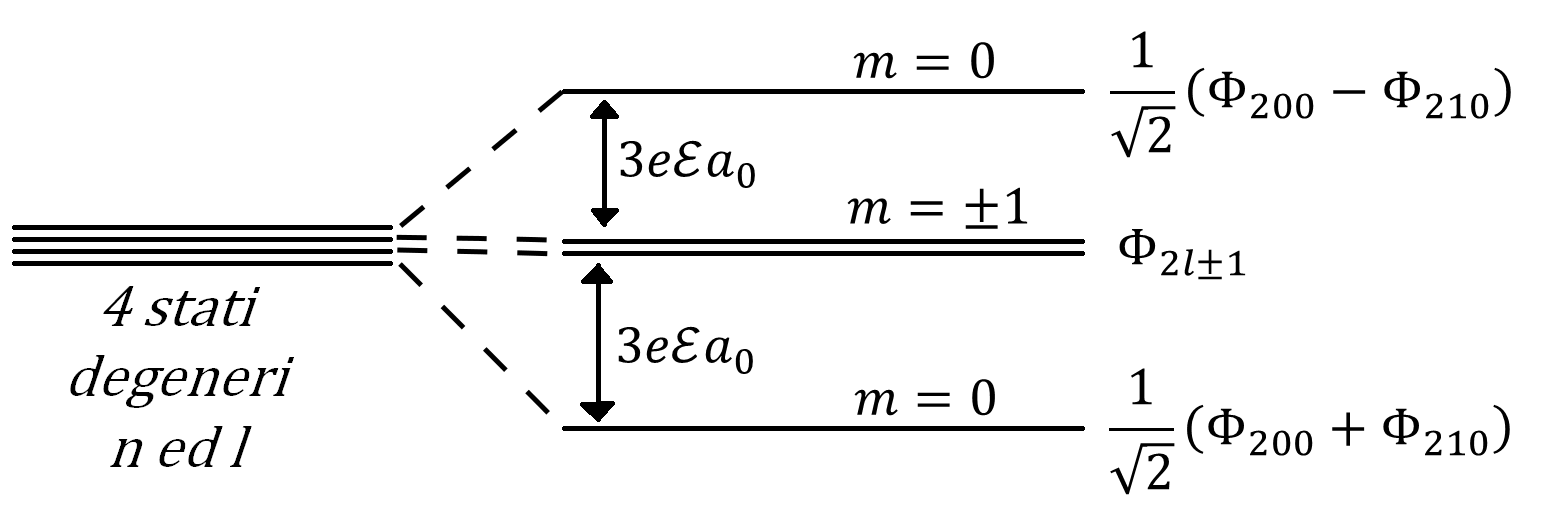
\includegraphics[width=10cm]{immagini/cap_23/fig23_1.png}
\end{center}
Poiché lo spostamento dei livelli, in prima approssimazione, è proporzionale al campo elettrico esterno $\mathcal{E}$, si parla in questo caso di $\textbf{effetto Stark lineare}$.\\
Osserviamo che, \textbf{in presenza del campo elettrico, gli autostati dell'hamiltoniana non sono più autostati di $\boldsymbol{L^2}$}. Ad esempio, nel sottospazio degli stati con $n=2$, abbiamo ottenuto combinazioni lineari di stati corrispondenti ad $l=0$ ed $l=1$. La ragione è che, in presenza del campo elettrico esterno, \textbf{il sistema non è più invariante per rotazioni arbitrarie, e l'hamiltoniana non commuta più con l'operatore momento angolare $\boldsymbol{L^2}$}.\\
Tuttavia, \textbf{il sistema è ancora invariante per rotazione attorno all'asse $\boldsymbol{z}$, che definisce la direzione del campo esterno. L'hamiltoniana perturbata commuta con la proiezione $\boldsymbol{L_z}$ del momento angolare orbitale e gli autostati di $\boldsymbol{H}$ sono simultaneamente autostati di $\boldsymbol{L_z}$}. %DEFINITIVO
\chapter[Atomo in un campo magnetico]{Atomo in un campo\\magnetico\footnote{G17; S5.3; LL113}}
Consideriamo un atomo di idrogeno o idrogenoide in un \textbf{campo magnetico omogeneo}.
Trascurando i termini quadratici nel campo esterno l'\textbf{hamiltoniano} si può scrivere nella forma:
\begin{equation} \label{eq:cap24_1}
H=H_0+H_{LS}+H_B ,
\end{equation}
dove
\begin{equation} \label{eq:cap24_2}
H_0=\frac{\vec{p^2}}{2m}+V_c(r) 
\end{equation}
è l'hamiltoniano dell'atomo in assenza di campo esterno e nel limite in cui si trascurano le correzioni di struttura fine,
\begin{equation} \label{eq:cap24_3}
H_{LS}=\frac{1}{2m^2c^2} \ \frac{1}{r} \ \frac{dV_c}{dr} \ \vec{L} \cdot \vec{S} ,
\end{equation}
rappresenta l'\textbf{interazione spin-orbita}, e
\begin{equation} \label{eq:cap24_4}
H_B=\frac{e}{2mc}\left( \vec{L}+2\vec{S} \right) \cdot \vec{B} 
\end{equation}
rappresenta l'\textbf{accoppiamento tra il momento magnetico dell'atomo e il campo esterno}
. \\
In questa trattazione ometteremo di considerare esplicitamente la correzione relativistica di struttura fine all'energia cinetica dell'elettrone in quanto non gioca alcun ruolo rilevante. Si può pensare di includere questa interazione nella hamiltoniana $H_0$

\section{Effetto Zeeman}
Supponiamo che il \textbf{campo magnetico} sia così \textbf{debole} che l'interazione ($H_0$) tra il momento magnetico dell'atomo ed il campo esterno risulti piccolo rispetto alle distanze fra i livelli energetici dell'atomo nonché rispetto agli intervalli della struttura fine dei livelli. \\
In questo caso il termine $H_B$ dell'hamiltoniana si può considerare come una perturbazione e lo spostamento dei livelli $\Delta E$ sarà determinato dal valore medio della perturbazione sugli stati "imperturbati" dell'hamiltoniana $H_0+H_{LS}$, ossia sugli autostati di $J^2$, $J_z$, $L^2$, $S^2$:
\begin{eqnarray} \label{eq:cap24_5}
\Delta E_B &=& \bra{\psi_{jm_jl}} H_B \ket{\psi_{jm_jl}}= \nonumber \\
& = &\frac{eB}{2mc} \bra{\psi_{j\ m_j\ l}} \left( L_z+2S_z \right)\ket{\psi_{j\ m_j\ l}}= \nonumber\\
& =& \frac{eB}{2mc} \bra{\psi_{j\ m_j\ l}} \left( J_z+S_z \right)\ket{\psi_{j\ m_j\ l}} ,
\end{eqnarray} 
dove si è scelto l'asse $z$ orientato nella direzione del campo esterno. \\
Il valore medio di $J_z$ coincide semplicemente con l'autovalore dato da $J_z=m_j$. Quanto al valore medio di $S_z$, questo può essere calcolato esplicitamente utilizzando le espressioni
\begin{eqnarray}
& & \mathcal{Y}_{j=l+1/2,m_j=m+1/2}=\sqrt{\frac{l+m+1}{2l+1}}Y_{lm}\chi_{+} + \sqrt{\frac{l-m}{2l+1}}Y_{l,m+1}\chi_{-} ,\\
&  &\mathcal{Y}_{j=l-1/2,m_j=m+1/2}=-\sqrt{\frac{l-m}{2l+1}}Y_{lm}\chi_{+} + \sqrt{\frac{l+m+1}{2l+1}}Y_{l,m+1}\chi_{-} .
\end{eqnarray}
Così per $j=l+1/2$ si ottiene:
\begin{eqnarray}
\langle S_z \rangle_{j=l+1/2,m_j=m+1/2} & =& \frac{\hbar}{2} \left( \frac{l+m+1}{2l+1}-\frac{l-m}{2l+1} \right)=\frac{\hbar}{2} \ \frac{2m+1}{2l+1}=  \nonumber \\
& = & \frac{\hbar m_j}{2l+1} ,
\end{eqnarray}
e per $j=l-1/2$:
\begin{eqnarray}
\langle S_z \rangle_{j=l-1/2,m_j=m+1/2} & = &\frac{\hbar}{2} \left( \frac{l-m}{2l+1}-\frac{l+m+1}{2l+1} \right)=-\frac{\hbar}{2} \ \frac{2m+1}{2l+1}=  \nonumber \\
& =& -\frac{\hbar m_j}{2l+1} .
\end{eqnarray}
In questo modo, sostituendo i precedenti risultati nell'equazione (\ref{eq:cap24_5}) otteniamo, per gli \textbf{spostamenti} dei livelli dovuti al campo magnetico la formula
\begin{equation} \label{eq:cap24_6}
\Delta E_B= \mu_B B m_j \left( 1\pm \frac{1}{2l+1}\right), \qquad j=l\pm 1/2 ,
\end{equation}
detta \textbf{formula di Landè} ($\mu_B=e\hbar /2mc$ è il magnetone di Bohr).
Così \textbf{il campo magnetico rimuove completamente la degenerazione dei livelli rispetto alle correzioni del momento angolare totale}, come indicata nello schema sottostante: 
\begin{center}
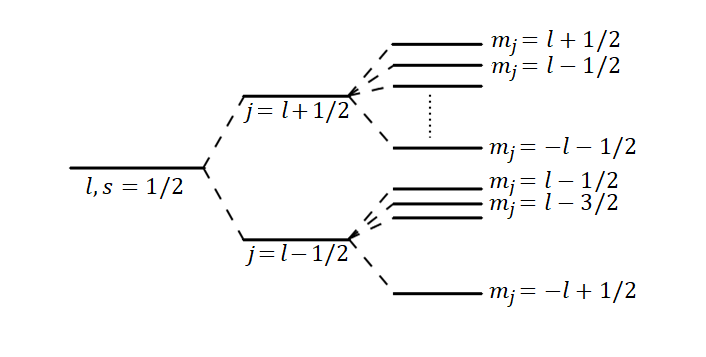
\includegraphics[width=10cm]{immagini/cap_24/fig24_1.png}
\end{center}

La separazione dei livelli indotta dal campo magnetico è nota come \textbf{effetto Zeeman}. \\
Talvolta si parla anche di effetto Zeeman \textbf{anomalo}. Questa denominazione impropria è dovuta storicamente al fatto che, ci si aspettava una separazione dei livelli determinata da $\Delta E_B=\mu_BBm$ in luogo della (\ref{eq:cap24_6}).

\section{Effetto Paschen-Back}
In \textbf{campi magnetici intensi}, in cui $\mu_B B$ è paragonabile agli intervalli della struttura fine o è addirittura più grande, la separazione dei livelli non segue quella prevista dalla formula ($\ref{eq:cap24_6}$). Questo fenomeno è detto \textbf{effetto Paschen-Back}. \\
Il calcolo dell'energia di separazione è assai semplice nel caso in cui la \textbf{separazione dei livelli è grande rispetto agli intervalli della struttura fine}, ma sempre piccola, s'intende, rispetto alle distanze dei livelli in assenza di campo esterno. \\
In queste caso è possibile trascurare, in prima approssimazione, l'accoppiamento spin-orbita e considerare $ H_0+H_B $ come hamiltoniana impterturbata. Questa hamiltoniana commuta con gli operatori \textbf{$\boldsymbol{L_z}$ ed $\boldsymbol{S_z}$}, proiezioni del momento angolare orbitale e dello spin nella direzione individuata dal campo esterno, che rappresentano pertanto \textbf{due buoni numeri quantici}. \\
Lo spostamento dei livelli allora può essere facilmente calcolato: 
\begin{eqnarray}
\Delta E_B & = &\bra{\phi_{lm_lm_s}} H_B \ket{\phi_{lm_lm_s}}=\nonumber  \\
& =& \frac{eB}{2mc}\bra{\phi_{lm_lm_s}} \left( L_z+2S_z  \right)\ket{\phi_{lm_lm_s}} ,
\end{eqnarray}
ossia 
\begin{equation}
\Delta E_B = \mu_B B \left( m_l+2m_s\right) .
\end{equation}
La degenerazione dei livelli che si aveva come l'hamiltonana $H_0$ è ora ridotta dal campo magnetico agli stati che hanno lo stesso valore di ($m_l+2m_s$). \\
\textbf{La struttura fine si sovrappone alla separazione nel campo magnetico}. Essa viene determinata dal valore medio dell'operatore $H_{LS}$ rispetto agli stati con $m_l$ ed $m_s$ determinati:
\begin{eqnarray}
\Delta E_{LS} & =& \bra{\phi_{lm_lm_s}} H_{LS} \ket{\phi_{lm_lm_s}}= \nonumber \\
& = &\frac{1}{2mc^2} \langle \frac{1}{r} \ \frac{dV_c}{dr}   \rangle \bra{lm_Lm_S} \vec{L} \cdot \vec{S} \ket{lm_Lm_S} .
\end{eqnarray}
Utilizzando l'identità:
\begin{eqnarray}
\vec{L} \cdot \vec{S} & = & L_xS_x+L_yS_y+L_zS_z= \nonumber  \\
& = & \frac{1}{4} \left( L_{+}+L_{-} \right)  \left( S_{+}+S_{-}\right)-\frac{1}{4} \left( L_{+}-L_{-} \right) \left( S_{+}-S_{-} \right)+L_zS_z =  \nonumber \\
& = &\frac{1}{2} \left( L_{+}S_{-}+L_{-}S_{+} \right)+ L_zS_z ,
\end{eqnarray}
otteniamo
\begin{equation}
\Delta E_{LS}= \frac{\hbar^2}{2mc^2} \langle \frac{1}{r} \ \frac{dV_c}{dr}   \rangle m_lm_s .
\end{equation} %DEFINITIVO
\chapter[Correzioni relativistiche all'atomo di idrogeno]{Correzioni relativistiche\\ all'hamiltoniano\\ dell'atomo di idrogeno\footnote{G17, S5.3}}

La trattazione fatta dell'atomo di idrogeno era basata sull'hamiltoniana
\begin{equation} \label{eq:cap25_1}
H_0=\frac{\vec{p^2}}{2m}-\frac{\mathcal{Z} e^2}{r}
\end{equation}
($\mathcal{Z}=1$ per l'atomo di idrogeno). In una trattazione più realistica è necessario prendere in considerazione diverse \textbf{correzioni}.

\section{Termine cinetico}

L'espressione dell'\textbf{energia cinetica} dell'elettrone si modifica quando si considerano \textbf{correzioni relativistiche }. Nella meccanica relativistica l'energia cinetica è data da:

\begin{eqnarray} 
E & = &\sqrt{m^2c^4+c^2\vec{p^2}}= mc^2 \sqrt{1+ \frac{\vec{p^2}}{m^2c^2}} \simeq \nonumber  \\
& \simeq & mc^2 \left( 1+ \frac{\vec{p^2}}{2m^2c^2}-\frac{(\vec{p^2})^2}{8m^4c^4}+\dots \right) = \nonumber  \\
& = & mc^2+\frac{\vec{p^2}}{2m}-\frac{(\vec{p^2})^2}{8m^3c^2}+ \dots 
\end{eqnarray}
Il termine della massa a riposo rappresenta una costante additiva irrilevante nella definizione dell'energia. La prima correzione relativistica è allora data dal termine 
\begin{equation} \label{eq:cap25_2}
H_1=-\frac{(\vec{p^2})^2}{8m^3c^2} ,
\end{equation}
che deve essere aggiunto all'hamiltoniana $H_0$. \\
Una stima dell'effetto di questa correzione sui livelli di energia dell'atomo può essere ottenuto utilizzando il principio di indeterminazione ed assumendo come valore approssimato del raggio dell'orbita \textbf{elettronica il valore $\boldsymbol{a_0\mathcal{Z}}$}. Si ottiene in tal modo
\begin{equation} 
\frac{\left< H_1 \right>}{\langle H_0 \rangle} \approx \frac{\vec{p^2}}{m^2c^2} \simeq \frac{\hbar^2 \mathcal{Z}^2}{m^2c^2a_0^2}=\frac{\mathcal{Z}^2 \hbar^2}{m^2c^2} \left( \frac{me^2}{\hbar^2}\right)^2=\frac{\mathcal{Z}^2 e^4}{\hbar^2 c^2} ,
\end{equation}
ossia
\begin{equation} 
\frac{\left< H_1 \right>}{\langle H_0 \rangle} \approx \left( \frac{v_e}{c} \right)^2 \approx \left(  \mathcal{Z} \alpha \right)^2 ,
\end{equation}
dove
\begin{equation} 
\alpha=\frac{e^2}{\hbar c} \simeq \frac{1}{137}
\end{equation}
è la cosiddetta costante di struttura fine. \\ Così, per l'atomo di idrogeno, questa correzione relativistica è dell'ordine di grandezza relativo di $\sim10^{-4}$.
\section{Accoppiamento spin-orbita}

L'\textbf{esistenza dello spin} dell'elettrone implica un'altra \textbf{correzione dello stesso ordine di grandezza}. Questa può essere qualitativamente compresa col seguente ragionamento: se l'elettrone fosse in quiete rispetto al protone, risentirebbe solo di un campo elettrico generato dalla carica del protone. Questo è il \textbf{termine del potenziale di Coulomb che appare in $\boldsymbol{H_0}$}. Poiché l'elettrone è però in movimento vi sono effetti addizionali. \\
\textbf{Nel sistema di riferimento dell'elettrone, il protone è in moto così che è presente una corrente e l'elettrone risente di un campo magnetico. Questo campo magnetico interagisce con lo spin dell'elettrone, o, più precisamente, con il momento magnetico dell'elettrone}. \\
Se il moto relativo del protone rispetto all'elettrone fosse rettilineo, il campo magnetico visto dall'elettrone sarebbe dato da:
\begin{equation} 
\vec{B}^{'}=-\gamma \frac{\vec{v}}{c} \wedge \vec{E} \ \simeq -\frac{\vec{v}}{c} \wedge \vec{E} ,
\end{equation}
dove $\vec{E}$ è il campo elettrico nel sistema di quiete del protone. \\
Poiché l'elettrone ha un momento magnetico intrinseco proporzionale al suo spin, dalla forma
\begin{equation} 
\vec{\mu}=-\frac{e}{mc}\vec{S} 
\end{equation}
ci aspettiamo che l'interazione con il campo magnetico effettivo risulti data da
\begin{eqnarray}
H_2 & =& -\vec{\mu} \cdot \vec{B}^{'}=\frac{e}{mc} \vec{S} \cdot \vec{B}^{'}= -\frac{e}{mc^2}\vec{S} \cdot \left( \vec{v} \wedge \vec{E} \right)= \nonumber \\
& =& + \frac{e}{m^2c^2}\vec{S} \cdot \vec{p} \wedge \vec{\nabla}\phi= \frac{e}{m^2c^2}\vec{S} \cdot \vec{p} \wedge \frac{\vec{r}}{r} \ \frac{d\phi}{dr}= \nonumber \\
& = &-\frac{e}{m^2c^2}\frac{1}{r} \ \frac{d\phi}{dr}\vec{S} \cdot \vec{L}= \frac{1}{m^2c^2} \left( \frac{1}{r} \ \frac{dV}{dr} \right) \vec{S} \cdot \vec{L} ,
\end{eqnarray}

dove $V=-e\phi=-\mathcal{Z}e^2/r$ è il potenziale cui è soggetto l'elettrone. \\
In realtà il moto dell'elettrone non è rettilineo uniforme, ed il risultato ottenuto risulta troppo grande di un fattore $2$ (\textbf{questo effetto è noto come precessione di Thomas}. Il termine di interazione corretto ha dunque la forma
\begin{equation} \label{eq:cap25_3}
H_2=\frac{1}{2m^2c^2} \left( \frac{1}{r} \ \frac{dV}{dr} \right) \vec{S} \cdot \vec{L} ,
\end{equation}
con
\begin{equation} 
V=-\frac{\mathcal{Z}e^2}{r} .
\end{equation}
Anche in questo caso è semplice ottenere una \textbf{stima della correzione} indotta dal termine aggiuntivo nell'hamiltoniana:
\begin{eqnarray}
\frac{\left< H_2 \right>}{\langle H_0 \rangle} & \approx & \frac{1}{m^2c^2} \left( \frac{1}{r} \ \frac{\mathcal{Z}e^2}{r^2} \right) \vec{S} \cdot \vec{L} \cdot \left( \frac{\mathcal{Z}e^2}{r} \right)^{-1} \approx \nonumber  \\
& \approx &\frac{\vec{S} \cdot \vec{L}}{m^2c^2r^2} \approx  \frac{\hbar^2 \mathcal{Z}^2}{m^2c^2a_0^2}=  \frac{\mathcal{Z}^2 \hbar^2}{m^2c^2}\left( \frac{me^2}{\hbar^2} \right)^2= \frac{\mathcal{Z}^2e^4}{\hbar^2c^2} ,
\end{eqnarray}
ossia
\begin{equation} 
\frac{\left< H_2 \right>}{\langle H_0 \rangle} \approx \left( \mathcal{Z}\alpha \right)^2 .
\end{equation}
L'interazione spin-orbita induce pertanto una correzione relativa ai livelli energetici dell'atomo che è dello stesso ordine di grandezza della correzione relativistica dovuta al termine cinematico ($\sim10^{-4}$ per $\mathcal{Z}=1$).
\section{Calcolo perturbativo delle correzioni}

L'effetto stimato delle correzioni ai livelli energetici degli atomo idrogenoidi, indotto dalla correzione relativistica all'energia cinetica e dell'accoppiamento spin-orbita, è sufficientemente piccolo da poter essere trattato, con ottima approssimazione, nella \textbf{teoria delle perturbazioni}. \\
Consideriamo come hamiltoniana imperturbata l'hamiltoniana $H_0$ dell'equazione (\ref{eq:cap25_1}) e come perturbazione $V$ la somma delle hamiltoniane $H_1$ e $H_2$ definite in equazione (\ref{eq:cap25_2}) e (\ref{eq:cap25_3}):
\begin{equation} 
V=H_1+H_2=-\frac{p^4}{8m^3c^2}+\frac{1}{2m^2c^2} \left( \frac{1}{r} \ \frac{dV}{dr} \right) \vec{S} \cdot \vec{L} .
\end{equation}
Proponiamoci qui di calcolare le \textbf{correzioni ai livelli energetici imperturbati, al primo ordine nella perturbazione $\boldsymbol{V}$}. \\
I livelli di energia dell'hamiltoniana imperturbata $H_0$, corrispondenti ad un determinato valore del numero quantico principale $n$, hanno un grado di degenerazione pari a $2n^2$. Gli stati degeneri differiscono per i diversi valori dei numeri quantici $l,m_l$ ed $m_s$ definiti dagli autovalori di $L^2$, $L_z$ ed $S_z$. Per tutti gli stati con $n>1$ risulta quindi necessario applicare la \textbf{teoria delle perturbazioni nel caso degenere}. \\
Il calcolo risulta estremamente semplificato se, per quanto concerne la dipendenza delle variabili angolari e di spin delle funzioni d'onda imperturbate, si considerano gli \textbf{autostati di}
\begin{equation} \label{eq:cap25_4}
J^2, \ J_x, \ L^2, \ S^2 ,
\end{equation}
in luogo degli autostati di $L^2, L_z, S^2, S_z$. \\
Le perturbazioni $H_1$ ed $H_2$ possono infatti essere scritte convenientemente nella forma
\begin{equation} \label{eq:cap25_5}
H_1=-\frac{1}{2mc^2} \left( \frac{\vec{p^2}}{2m} \right)^2 = -\frac{1}{2mc^2} \left( H_0+\frac{\mathcal{Z}e^2}{r} \right)^2 ,
\end{equation}
e
\begin{equation} \label{eq:cap25_6}
H_2=\frac{1}{4m^2c^2} \left( \frac{1}{r} \ \frac{dV}{dr} \right) \left(\vec{J}^2-\vec{L}^2-\vec{S}^2 \right) .
\end{equation}
Da queste espressioni risulta infatti evidente che \textbf{gli operatori $\boldsymbol{H_1}$ ed $\boldsymbol{H_2}$ commutano con gli operatori in equazione (\ref{eq:cap25_4}), cosicché, nella corrispondente base, la perturbazione risulta già diagonale}. \\ (\'E bene sottolineare, tuttavia, che le perturbazioni $H_1$ ed $H_2$ non commutano, ovviamente, con l'hamiltoniano imperturbato $H_0$. Pertanto $H_1$ ed $H_2$ risultano diagonali solo nel sottospazio degli autostati degeneri di $H_0$ corrispondenti a diversi valori di $J^2$, $J_z$ ed $L^2$). \\
\textbf{Le correzioni al primo ordine ai livelli energetici dell'atomo si ottengono allora direttamente calcolando i valori di aspettazione della perturbazione $\boldsymbol{V}$ sugli autostati di $\boldsymbol{H_0}$, $\boldsymbol{J^2}$, $\boldsymbol{J_z}$, $\boldsymbol{L^2}$, $\boldsymbol{S^2}$}. \textbf{Indichiamo questi autostati con}
\begin{equation} 
| n,l,j,m_j \rangle .
\end{equation}
Per un determinato valore del numero quantico orbitale $l$, il numero quantico $j$ può assumere i valori
\begin{equation} 
j=l\pm1/2 .
\end{equation}
Le corrispondenti autofunzioni sono della forma
\begin{equation} 
\psi_{n,l,j,m_j}=R_{nl}(r)Y_{j=l\pm1/2,m_j} .
\end{equation}
Cominciamo con il calcolare, su questi stati, \textbf{i valori medi della perturbazione $\boldsymbol{H_1}$} indotta dalle correzioni relativistiche all'energia cinetica. Utilizziamo l'equazione ($\ref{eq:cap25_5}$) troviamo:
\begin{eqnarray} \label{eq:cap25_7} 
& &\langle n,l,j,m_j | H_1 |n,l,j,m_j \rangle = \nonumber \\
& &=-\frac{1}{2mc^2}\langle n,l,j,m_j |\left( H_0+\frac{\mathcal{Z}e^2}{r} \right) \left( H_0+\frac{\mathcal{Z}e^2}{r} \right)  |n,l,j,m_j \rangle = \nonumber \\
& &=-\frac{1}{2mc^2}\langle n,l,j,m_j | \left( E_n+\frac{\mathcal{Z}e^2}{r} \right)^2  | n,l,j,m_j\rangle = \nonumber \\
& &=-\frac{1}{2mc^2} \left( E_n^2+2E_n\mathcal{Z}e^2 \left< \frac{1}{r} \right>_{nl} +\left( \mathcal{Z}e^2 \right)^2\left< \frac{1}{r^2} \right>_{nl} \right)  ,
\end{eqnarray}
dove si sono definiti i valori medi
\begin{eqnarray} 
\left< \frac{1}{r^k} \right>_{nl} & = \langle n,l,j,m_j | \frac{1}{r^k} | n,l,j,m_j \rangle = \nonumber\\
& = \int_0^{\infty} dr \ r^2 \ \frac{1}{r^k} \left( R_{nl}(r) \right)^2 .
\end{eqnarray}
Per questi valori medi sono note delle formule generali, che qui riportiamo:
\begin{equation} \label{eq:cap25_8}
\begin{split}
\left< \frac{1}{r} \right>_{nl} & = \left( \frac{\mathcal{Z}}{a_0} \right) \frac{1}{n^2} , \\ 
\left< \frac{1}{r^2} \right>_{nl} & = \left( \frac{\mathcal{Z}}{a_0} \right)^2 \frac{1}{n^3(l+1/2)}  ,\\ 
\left< \frac{1}{r^3} \right>_{nl} &= \left( \frac{\mathcal{Z}}{a_0} \right)^3 \frac{1}{n^3 \ l \ (l+1/2)(l+1)} \qquad (l \neq0) .
\end{split}
\end{equation}
(Il valor medio $\left<1/r^3\right>_{nl}$ risulterà utile nel calcolo della correzione indotta dall'accoppiamento spin-orbita). \\
Sostituendo i valori medi (\ref{eq:cap25_8}) nell'equazione (\ref{eq:cap25_7}) ed utilizzando le espressioni
\begin{equation} 
E_n=-\frac{mc^2 \left(\mathcal{Z}\alpha\right)^2}{2n^2} 
\end{equation}
per l'energia dei livelli imperturbati e 
\begin{equation} 
a_0=\frac{\hbar^2}{me^2}=\frac{\hbar^2c^2}{e^4}\frac{e^2}{mc^2}=\frac{e^2}{mc^2\alpha^2}
\end{equation}
per il raggio di Bohr, otteniamo:

\begin{eqnarray} 
 \left< H_1 \right>_{nljm_j} & =& -\frac{1}{2mc^2} \left[ \frac{m^2c^4 \left( \mathcal{Z} \alpha \right)^4}{4n^4}-\frac{mc^2 \left( \mathcal{Z} \alpha \right)^2 \mathcal{Z} e^2}{n^4} \frac{mc^2\alpha^2 \mathcal{Z}}{e^2}+ \right. \nonumber \\
& &\left. + \left( \mathcal{Z} e^2 \right)^2 \frac{1}{n^3(l+1/2)} \left(\frac{mc^2\alpha^2}{e^2} \right)^2 \mathcal{Z}^2 \right] = \nonumber  \\
& = & -\frac{1}{2mc^2} \left( m^2c^4 \right) \left( \mathcal{Z} \alpha\right)^4 \left[ \frac{1}{4n^4}-\frac{1}{n^4}+\frac{1}{n^3(l+1/2)}  \right] ,
\end{eqnarray}
ossia
\begin{equation} \label{eq:cap25_9}
\left< H_1 \right>_{nljm_j} = -\frac{1}{2}mc^2 \left( \mathcal{Z} \alpha \right)^4 \left[ \frac{1}{n^3(l+1/2)}-\frac{3}{4n^4}\right]  .
\end{equation}
Questa correzione risulta dall'ordine di grandezza aspettato: più piccola di circa un fattore $\left( \mathcal{Z} \alpha \right)^2$ rispetto ai livelli di energia imperturbati. \\
Calcoliamo ora la \textbf{correzione}, al primo ordine dello sviluppo perturbativo, \textbf{indotto} sui livelli di energia imperturbati \textbf{dall'interazione spin-orbita}. \\ 
Utilizzando l'equazione (\ref{eq:cap25_6}) otteniamo:
\begin{eqnarray} \label{eq:cap25_10}
\left< H_2 \right>_{nljm_j} &=& \langle n,l,j,m_j | H_2 | n,l,j,m_j \rangle = \nonumber  \\
& = &\frac{1}{4m^2c^2} \langle n,l,j,m_j | \left( \frac{\mathcal{Z}e^2}{r^3} \right) \left( \vec{J}^2-\vec{L}^2-\vec{S}^2 \right)      | n,l,j,m_j \rangle= \nonumber  \\
& = & \frac{\hbar^2\mathcal{Z}e^2}{4m^2c^2} \left< \frac{1}{r^3} \right>_{nl} \left[ j(j+1)-l(l+1)-\frac{3}{4}  \right] .
\end{eqnarray}
Il fattore tra parentesi quadre che entra in questa espressione, nei due casi $j=l\pm1/2$, vale 
\begin{eqnarray} 
& &\left. \left[ j(j+1)-l(l+1)-\frac{3}{4}  \right]  \right|_{j=l+1/2} = \nonumber \\ 
& &\qquad = \left( l+\frac{1}{2} \right) \left( l+\frac{3}{2}\right)-l\left(l+1 \right) -\frac{3}{4}=l
\end{eqnarray}
e
\begin{eqnarray} 
& &\left. \left[ j(j+1)-l(l+1)-\frac{3}{4}  \right] \right|_{j=l-1/2} = \nonumber  \\ 
& &\qquad = \left( l-\frac{1}{2} \right) \left(l+\frac{1}{2} \right)-l\left( l+1 \right) -\frac{3}{4}=-l-1 .
\end{eqnarray}
Sostituendo questi risultati nell'equazione (\ref{eq:cap25_10}), insieme al valore medio $\left< 1/r^3 \right>_{nl}$ dato nell'equazione (\ref{eq:cap25_8}), si ottiene:
\begin{equation} \label{eq:cap25_11}
\left< H_2 \right>_{nljm_j}=\frac{1}{4}mc^2\left( \mathcal{Z}\alpha \right)^4 \frac{\begin{Bmatrix}
      l  \\ 
      -l-1 
    \end{Bmatrix}
    \begin{matrix}
    \leftarrow j=l+1/2 \\
    \leftarrow j=l-1/2
    \end{matrix} }{n^3 \ l \ \left(l+1/2 \right) \left( l+1 \right)} ,
\end{equation}
valida per $l\neq0$. La correzione è nulla per $l=0$. \\
Le due correzioni, fornite dalle equazioni (\ref{eq:cap25_9}) e (\ref{eq:cap25_11}), possono essere infine combinate per ottenere la \textbf{correzione totale}, al primo ordine nella perturbazione, ai livelli di energia degli atomi idrogenoidi. Nei due casi, corrispondenti a $j=l\pm1/2$ si ottiene:

\begin{eqnarray} 
\left( \Delta E \right)_{j=l+1/2} &= & \left( \left< H_1\right> +\left<H_2 \right>  \right)_{j=l+1/2}= \nonumber \\
& =& -\frac{1}{2} mc^2 \left( \mathcal{Z}\alpha \right)^4 \frac{1}{n^3} \left[ \frac{1}{l+1/2}-\frac{3}{4n}-\frac{1}{2(l+1/2)(l+1)}\right]=  \nonumber \\
& = & -\frac{1}{2} mc^2 \left( \mathcal{Z}\alpha \right)^4 \frac{1}{n^3} \left[ \frac{l+1-1/2}{(l+1/2)(l+1)}-\frac{3}{4n}\right]= \nonumber  \\
& =v& -\frac{1}{2} mc^2 \left( \mathcal{Z}\alpha \right)^4 \frac{1}{n^3} \left[ \frac{1}{l+1}-\frac{3}{4n} \right]= \nonumber \\
& = &-\frac{1}{2} mc^2 \left( \mathcal{Z}\alpha \right)^4 \frac{1}{n^3} \left[ \frac{1}{j+1/2}-\frac{3}{4n} \right]
\end{eqnarray}
e
\begin{eqnarray} 
 \left( \Delta E \right)_{j=l-1/2}&=&\left( \left< H_1\right> +\left<H_2 \right>  \right)_{j=l-1/2}= \nonumber \\
& = &-\frac{1}{2} mc^2 \left( \mathcal{Z}\alpha \right)^4 \frac{1}{n^3} \left[ \frac{1}{l+1/2}-\frac{3}{4n}-\frac{1}{2l(l+1/2)}\right]= \nonumber \\
& =& -\frac{1}{2} mc^2 \left( \mathcal{Z}\alpha \right)^4 \frac{1}{n^3} \left[ \frac{l+1/2}{l(l+1/2)}-\frac{3}{4n}\right]= \nonumber \\
& = &-\frac{1}{2} mc^2 \left( \mathcal{Z}\alpha \right)^4 \frac{1}{n^3} \left[ \frac{1}{l}-\frac{3}{4n} \right]= \nonumber  \\
& = & -\frac{1}{2} mc^2 \left( \mathcal{Z}\alpha \right)^4 \frac{1}{n^3} \left[ \frac{1}{j+1/2}-\frac{3}{4n} \right] .
\end{eqnarray}
In conclusione, possiamo scrivere:
\begin{eqnarray}
\Delta E &=& \langle H_1+H_2 \rangle_{nljm_j}= \nonumber\\
& = &-\frac{1}{2}mc^2 \left( \mathcal{Z}\alpha \right)^4 \frac{1}{n^3} \left[ \frac{1}{j+1/2}-\frac{3}{4n}\right] ,
\end{eqnarray}
valida per entrambi i valori $j=l\pm1/2$. \\
Utilizzando l'equazione relativistica di Dirac è possibile mostrare che il risultato ottenuto è corretto anche nel caso \textbf{$\boldsymbol{l=0}$}. \\
Lo splitting dei livelli è rappresentato, per il caso $n=2$, nello schema sottostante\\
\begin{center}
\includegraphics[width=10cm]{immagini/cap_25/fig25_1.png}
\end{center}
Gli stati con $l=1$ (stati $p$) possono avere $j=1/2$ e $j=3/2$ mentre gli stati con $l=0$ (stati $s$) corrispondono necessariamente a $j=1/2$. \'E interessante osservare le correzioni dovute allo spin-orbita e al termine cinetico si sommano in modo tale da rendere degeneri gli stati $^2S_{1/2}$ e $^2P_{1/2}$.
Una trattazione più accurata, basata sull'equazione relativistica di Dirac, non altera questo risultato. Tuttavia, nel $1947$, un accurato esperimento condotto da Lamb e Rutherford ha mostrato una sottile separazione tra i due livelli $^2S_{1/2}$ e $^2P_{1/2}$ (\textbf{Lamb-shift}). Questo effetto è spiegabile soltanto nel contesto della completa teoria quantistica relativistica ed è originato dalle fluttuazioni quantistiche del campo dell'elettrone. %DEFINITIVO
\end{document}